\documentclass{article}
\usepackage[utf8]{inputenc}
\usepackage{graphicx}
\usepackage{caption}
\usepackage{placeins}
\usepackage{natbib}
\usepackage{amsmath}
\usepackage{subfig}
\usepackage{verbatim}

% Packages to display eighth-core maps
\usepackage{amsfonts}
\usepackage{geometry}
\usepackage{color}
\usepackage{xcolor}
\usepackage{framed}
\usepackage{tabularx}
\usepackage{setspace}
\PassOptionsToPackage{normalem}{ulem}
\usepackage{ulem}
\usepackage{tikz}
\usetikzlibrary{matrix,calc}
\usepackage{xstring,xspace}
\usepackage{multirow}
\usepackage{hyperref}


%\usepackage{etoolbox}
\usepackage{booktabs}   % For table definitions
\usepackage{enumitem}   % For enumerate
%\usepackage{tocloft}
%\usepackage[pdfborder={0 0 0}]{hyperref}
%\usepackage{microtype}                     % Improve typography

% Algorithm constructs
\usepackage[]{algorithm} % Provides algorithm environment
\usepackage{algorithmicx}       % Provides algorithmic block
\usepackage{algpseudocode}      % Option of algorithmicx package

\newcolumntype{B}{>{\centering\let\newline\\\arraybackslash\hspace{0pt}}m{2.65in}} % For 2 Column Table
\newcolumntype{C}{>{\centering\let\newline\\\arraybackslash\hspace{0pt}}m{1.77in}} % For 3 Column Table
\newcolumntype{D}{>{\centering\let\newline\\\arraybackslash\hspace{0pt}}m{1.33in}} % For 4 Column Table
\newcolumntype{E}{>{\centering\let\newline\\\arraybackslash\hspace{0pt}}m{1.38in}} % For 4 Column Table Wide
\newcolumntype{F}{>{\centering\let\newline\\\arraybackslash\hspace{0pt}}m{1.45in}} % For 4 Column Table Wide
\newcolumntype{G}{>{\centering\let\newline\\\arraybackslash\hspace{0pt}}m{1.06in}} % For 5 Column Table
\newcolumntype{H}{>{\centering\let\newline\\\arraybackslash\hspace{0pt}}m{1.45in}} % For 4 Column Table with Narrow First Column
\newcolumntype{I}{>{\centering\let\newline\\\arraybackslash\hspace{0pt}}m{0.96in}} % For Narrow First Column in 4 Column Table


\title{Integral Full Core Multi-Physics PWR \\
Benchmark with Measured Data \\
NEUP 14-6742: Final Report}
\author{Shikhar Kumar, Jingang Liang, Miriam Rathbun, Benoit Forget, Kord Smith}
\date{April 11, 2018}

\begin{document}

\maketitle

\section{Introduction}

In recent years, the importance of modeling and simulation has been highlighted extensively in the DOE research portfolio with concrete examples in nuclear engineering with the CASL and NEAMS programs.  These research efforts and similar efforts worldwide aim at the development of high-fidelity multi-physics analysis tools for the simulation of current and next-generation nuclear power reactors.  Like all analysis tools, verification and validation is essential to guarantee proper functioning of the software and methods employed.  The current approach relies mainly on the validation of single physic phenomena (e.g. critical experiment, flow loops, etc.) and there is a lack of relevant multiphysics benchmark measurements that are necessary to validate high-fidelity methods being developed today.

This work introduces a new multi-cycle full-core Pressurized Water Reactor (PWR) depletion benchmark based on two operational cycles of a commercial nuclear power plant that provides a detailed description of fuel assemblies, burnable absorbers, in-core fission detectors, core loading and re-loading patterns. This benchmark enables analysts to develop extremely detailed reactor core models that can be used for testing and validation of coupled neutron transport, thermal-hydraulics, and fuel isotopic depletion. The benchmark also provides measured reactor data for Hot Zero Power (HZP) physics tests, boron letdown curves, and three-dimensional in-core flux maps from 58 instrumented assemblies.  The benchmark description is now available online and has been used by many groups. However, much work remains to be done on the quantification of uncertainties and modeling sensitivities.  This work aims to address these deficiencies and make this benchmark a true non-proprietary international benchmark for the validation of high-fidelity tools.

This report details the BEAVRS uncertainty quantification for the first two cycle of operations and serves as the final report of the project.

\section{Benchmark}

The BEAVRS benchmark (Benchmark for Evaluation And Validation of Reactor Simulations) represents a 4-loop Westinghouse plant with as much detail available in the open literature.  Core loadings and detector readings were provided by plant operators for the first two cycles of operation with all necessary details (i.e. as-fabricated fuel assembly loadings, burnable absorber pin layouts, operational histories and control rod positions, boron concentration).  The core contains 193 Westinghouse optimized fuel assemblies (OFA) each with 264 fuel rods, 24 guide tubes, and one instrument tube arranged in a 17x17 square lattice. First cycle fuel rods in each assembly consist of UO2 with U-235 enrichments of 1.6, 2.4, or 3.1 weight-percent enrichment, depending on location, as depicted in Figure \ref{fig:loading_pattern1}, which also indicates the number of dry annular burnable absorber rods occupying guide tubes.  Figure \ref{fig:loading_pattern2} presents the re-load shuffling pattern and fresh fuel loading for cycle 2. 

In this reactor plant, there are 58-instrumented assemblies in which one of six variable- mass, in-core fission chambers can be positioned.  Each detector passes through a common instrument tube, which is an essential step for the inter-normalization of detector signals. As measurements are taken, detectors are inserted into the core through instrumentation tubes in assemblies until the top of the fuel assembly is reached. Detector signals are then recorded as the detectors are pulled through the core at a constant speed. Thus, measurements represent an integral of signals over a recording interval and this data has been integrated into 61 axial data points for each instrumented assembly location. 

\begin{figure}[!htb]
\centering
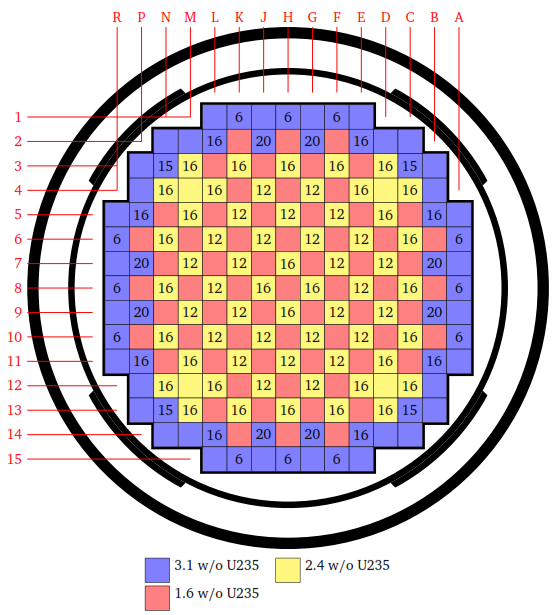
\includegraphics[width = 4.5 in]{figures/loading_pattern.png}
\caption{Cycle 1 Loading Pattern}
\label{fig:loading_pattern1}
\end{figure}

\begin{figure}[!htb]
\centering
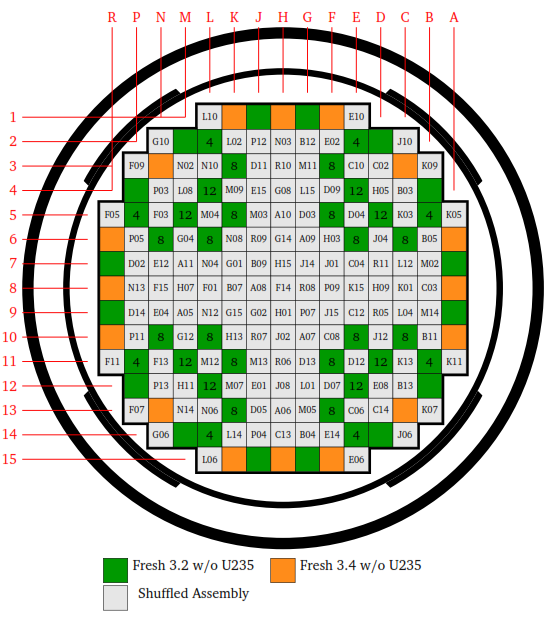
\includegraphics[width = 4.5 in]{figures/loading_pattern2.png}
\caption{Cycle 2 Loading Pattern}
\label{fig:loading_pattern2}
\end{figure}



Currently, the benchmark document provides detailed geometry for the 3D full core model for all non-proprietary data, and a few geometrical approximations have been made where proprietary data is unavailable.  All approximations are documented and are updated as new information is made available.  A Python processing script was developed to perform the necessary data filtering and normalization from the fission detectors data. A comprehensive methodology was proposed to quantifying the uncertainty of entire flux map, through estimating the uncertainty introduced in the filtering process and accuracy of detector signals by statistically analyzing the multiple measurements. Both the detailed axial and radial flux maps along with the uncertainties have been obtained and reported previously. For completeness, the process of generating these flux maps will be explained.

The first step in this process of generating radial reaction rate maps is to remove detector background signal. Next, the signal is multiplied by a gain factor to adjust the gain on the detectors. These gain factors are reported for each detector. Figure \ref{fig:orig_all} shows the initial raw detector measurements at Hot Zero Power (HZP), while Figure \ref{fig:gain_all} shows the measurements after correcting for background and applying gain factors. 

\begin{figure}[!htb]
    \centering
    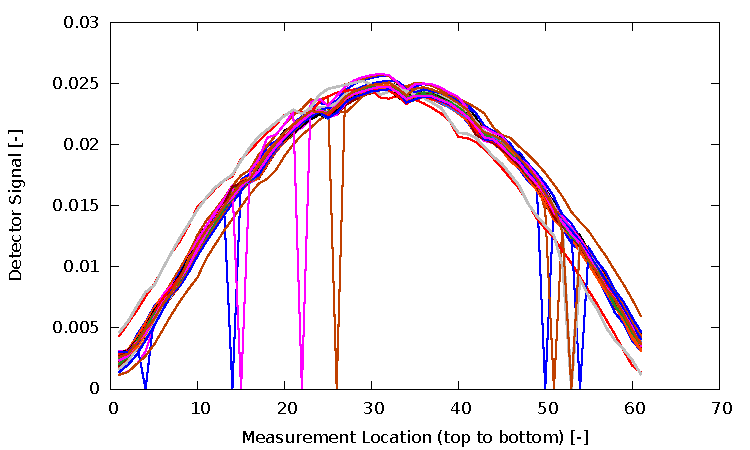
\includegraphics[width=4.5in]{figures/original_all.pdf}
    \caption{Initial raw detector measurements (top to bottom) \cite{beavrs}. \label{fig:orig_all}}
\end{figure}

\begin{figure}[!htb]
    \centering
    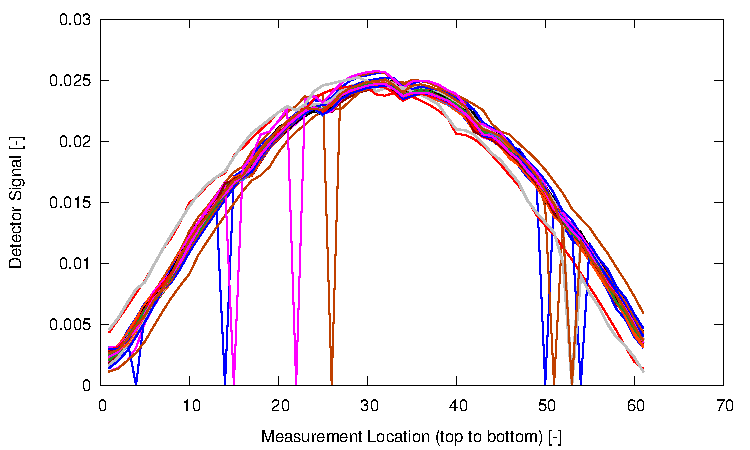
\includegraphics[width=4.5in]{figures/gain_all.pdf}
    \caption{Detector measurements with gain factors applied (top to bottom) \cite{beavrs}. \label{fig:gain_all}}
\end{figure}

Figure \ref{fig:gain_all} illustrates that zero points exist where detectors were unable to make measurements. Linear interpolation/extrapolation is used between/from the nearest two points to remove these zero points. The resulting data is shown in Figure \ref{fig:zero}. Within each detector pass, there are minor fluctuations in core power during the measurement, so the detector signal is divided by power during the measurement. Assembly J10 is the assembly where all detectors make a pass, so this is used for signal normalization purposes. Figure \ref{fig:J10} shows the detector measurements in assembly J10 at HZP. It is evident from this plot that each detector has a different signal intensity due to varying Uranium-235 mass in the fission chambers, despite each detector entering the same assembly. 

\begin{figure}[!htb]
    \centering
    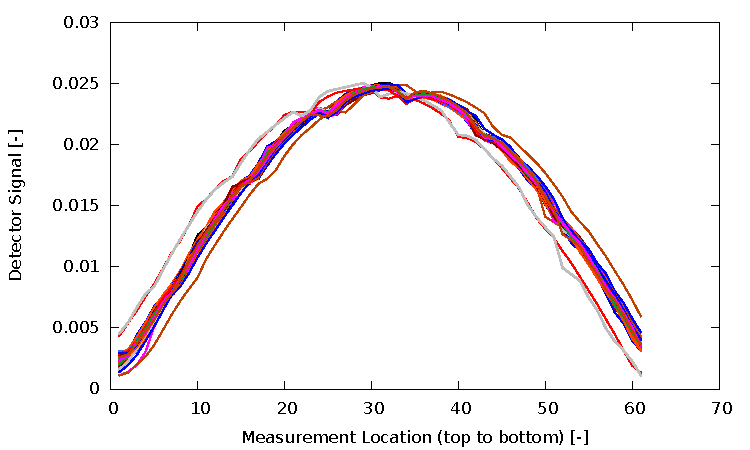
\includegraphics[width=4.5in]{figures/zeros_all.pdf}
    \caption{Detector measurements with zero points removed (top to bottom) \cite{beavrs}. \label{fig:zero}}
\end{figure}

\begin{figure}[!htb]
    \centering
    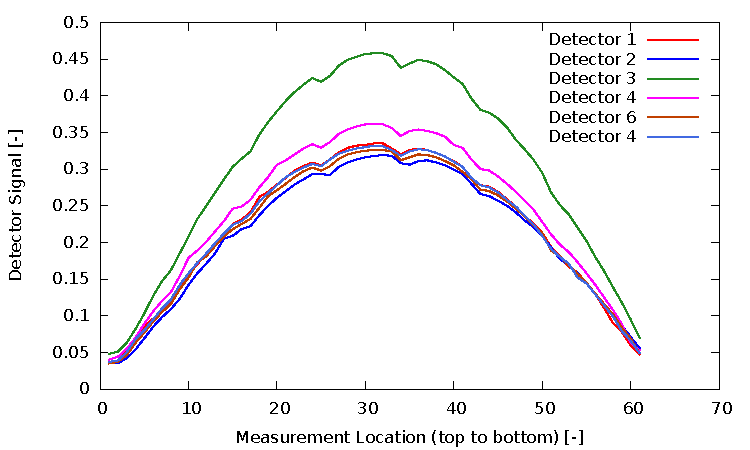
\includegraphics[width=4.5in]{figures/zeros.pdf}
    \caption{Detector measurements within assembly J10 (top to bottom) \cite{beavrs}. \label{fig:J10}}
\end{figure}

To account for this, each detector pass in each assembly is normalized to the signal strength of that specific detector in assembly J10. This allows all detector signals to have comparable shape functions. Figure \ref{fig:beforerealign} shows the detector signals at this stage. There is still some axial misalignment due to varying starting positions during recording, so the signals are subsequently aligned to grid depressions. The positions of these grid spacers are fixed, and Figure \ref{fig:afterrealign} presents the detector signals after realignment. The final step is to map the axial measurements from a grid system to a physical axial location on the active fuel. A second order spline fit is used to ensure that there are equal numbers of data points from the Top of Active Fuel (TAF) to the Bottom of Active Fuel (BAF). Figure \ref{fig:splineall} presents this data after the spline fit. The final measurements (no longer normalized to have the same shape functions)     are shown in Figure \ref{fig:splineunnorm}.


\begin{figure}[!htb]
    \centering
    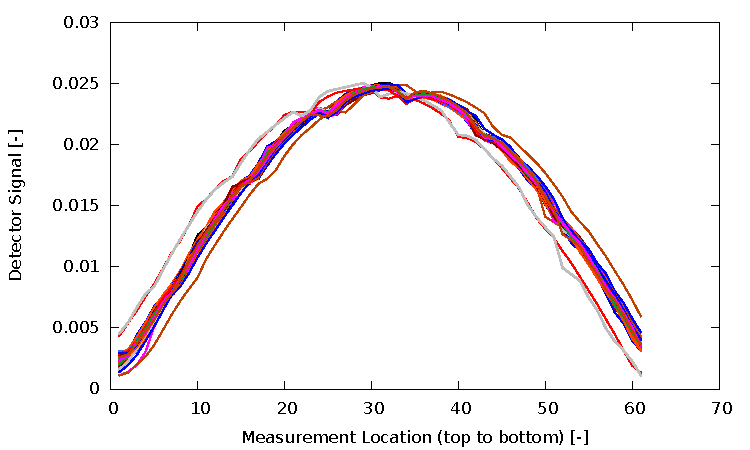
\includegraphics[width=4.5in]{figures/before_realign.pdf}
    \caption{All detector signals before realignment \cite{beavrs}.  \label{fig:beforerealign}}
\end{figure}

\begin{figure}[!htb]
    \centering
    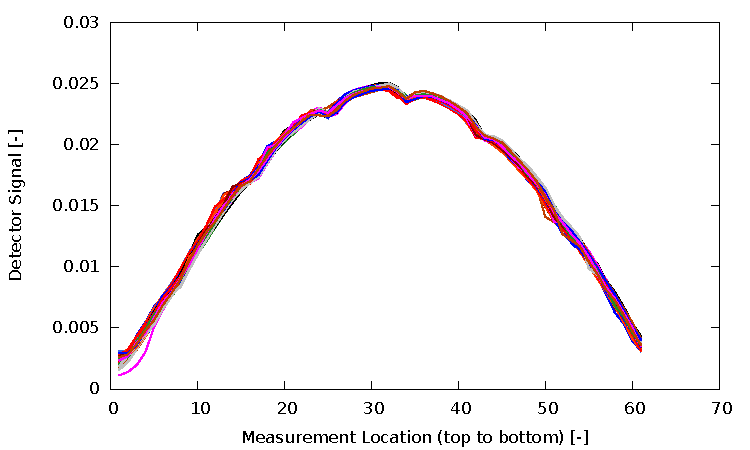
\includegraphics[width=4.5in]{figures/after_realign.pdf}
    \caption{All detector signals after realignment \cite{beavrs}. \label{fig:afterrealign}}
\end{figure}

\begin{figure}[!htb]
    \centering
    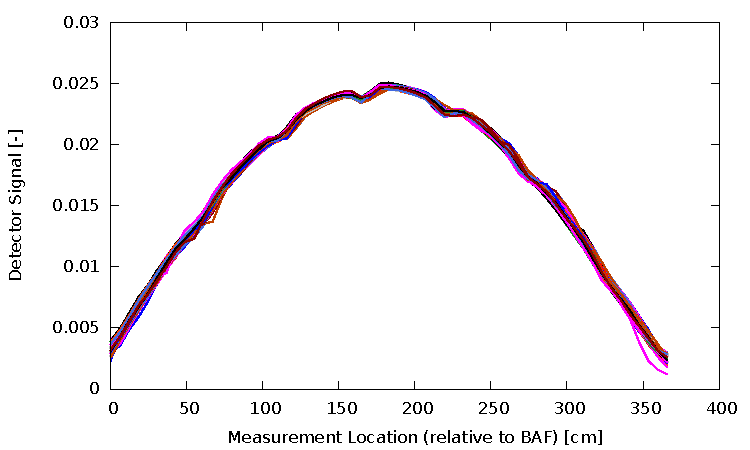
\includegraphics[width=4.5in]{figures/spline_all.pdf}
    \caption{Comparison of all assemblies after spline \cite{beavrs}. \label{fig:splineall}}
\end{figure}

\begin{figure}[!htb]
    \centering
    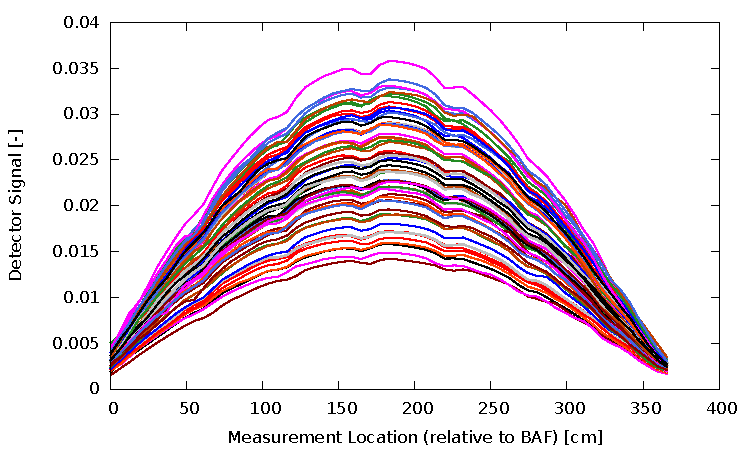
\includegraphics[width=4.5in]{figures/spline_unnorm.pdf}
    \caption{Final processed HZP measurement data \cite{beavrs}. \label{fig:splineunnorm}}
\end{figure}

With this data, axially integrated radial maps of fission reaction rates can now be created. The total sum of all signals in Figure \ref{fig:splineunnorm} is computed and renormalized to be equal to the total number of assemblies (for this particular case there are 58 assemblies where measurements occurred). Axially averaging each measurement in an assembly yields a relative radial peaking factor, and Figure \ref{fig:radial_meas} depicts this factor for each assembly where measurements were taken at HZP. While the specifics of this procedure focus only on data at HZP, the same processing algorithm has been done for all burnups where data is available \cite{beavrs}. It has also been shown that reaction rate maps generated by core simulation software are in close agreement with those shown in Figure \ref{fig:radial_meas} \cite{horelik2013}. 

\definecolor{Gsevencolor}{rgb}{1,1,1}
\definecolor{Gsixcolor}{rgb}{1,1,1}
\definecolor{Gfivecolor}{rgb}{0.8,0.618592167995,0.16}
\definecolor{Gfourcolor}{rgb}{1,1,1}
\definecolor{Gthreecolor}{rgb}{1,1,1}
\definecolor{Gtwocolor}{rgb}{1,1,1}
\definecolor{Gonecolor}{rgb}{1,1,1}
\definecolor{Gninecolor}{rgb}{0.8,0.784652300146,0.16}
\definecolor{Geightcolor}{rgb}{1,1,1}
\definecolor{Jeightcolor}{rgb}{0.454640153967,0.8,0.16}
\definecolor{Jninecolor}{rgb}{1,1,1}
\definecolor{Jfourcolor}{rgb}{1,1,1}
\definecolor{Jfivecolor}{rgb}{1,1,1}
\definecolor{Jsixcolor}{rgb}{1,1,1}
\definecolor{Jsevencolor}{rgb}{0.8,0.797530194246,0.16}
\definecolor{Jonecolor}{rgb}{0.459102226928,0.8,0.16}
\definecolor{Jtwocolor}{rgb}{1,1,1}
\definecolor{Jthreecolor}{rgb}{1,1,1}
\definecolor{Lfourteencolor}{rgb}{1,1,1}
\definecolor{Lfifteencolor}{rgb}{0.199325500465,0.8,0.16}
\definecolor{Ltencolor}{rgb}{0.736879753927,0.8,0.16}
\definecolor{Lelevencolor}{rgb}{0.8,0.418746058875,0.16}
\definecolor{Ltwelvecolor}{rgb}{1,1,1}
\definecolor{Lthirteencolor}{rgb}{0.8,0.306806119453,0.16}
\definecolor{Mfivecolor}{rgb}{1,1,1}
\definecolor{Mfourcolor}{rgb}{1,1,1}
\definecolor{Msevencolor}{rgb}{0.676919670852,0.8,0.16}
\definecolor{Msixcolor}{rgb}{1,1,1}
\definecolor{Mthreecolor}{rgb}{1,1,1}
\definecolor{Mtwocolor}{rgb}{1,1,1}
\definecolor{Mninecolor}{rgb}{1,1,1}
\definecolor{Meightcolor}{rgb}{1,1,1}
\definecolor{Ptencolor}{rgb}{1,1,1}
\definecolor{Pelevencolor}{rgb}{1,1,1}
\definecolor{Ptwelvecolor}{rgb}{1,1,1}
\definecolor{Pthirteencolor}{rgb}{1,1,1}
\definecolor{Peightcolor}{rgb}{1,1,1}
\definecolor{Pthreecolor}{rgb}{1,1,1}
\definecolor{Pninecolor}{rgb}{0.547691836697,0.8,0.16}
\definecolor{Psixcolor}{rgb}{1,1,1}
\definecolor{Psevencolor}{rgb}{1,1,1}
\definecolor{Pfourcolor}{rgb}{0.604342827129,0.8,0.16}
\definecolor{Pfivecolor}{rgb}{1,1,1}
\definecolor{Htencolor}{rgb}{1,1,1}
\definecolor{Helevencolor}{rgb}{0.743521203429,0.8,0.16}
\definecolor{Htwelvecolor}{rgb}{1,1,1}
\definecolor{Hthirteencolor}{rgb}{0.76691352318,0.8,0.16}
\definecolor{Hfourteencolor}{rgb}{1,1,1}
\definecolor{Hfifteencolor}{rgb}{0.548211017514,0.8,0.16}
\definecolor{Kthirteencolor}{rgb}{1,1,1}
\definecolor{Ktwelvecolor}{rgb}{0.8,0.478965220928,0.16}
\definecolor{Kelevencolor}{rgb}{1,1,1}
\definecolor{Ktencolor}{rgb}{1,1,1}
\definecolor{Dtencolor}{rgb}{0.8,0.378816128792,0.16}
\definecolor{Delevencolor}{rgb}{1,1,1}
\definecolor{Dtwelvecolor}{rgb}{0.8,0.16,0.16}
\definecolor{Dthirteencolor}{rgb}{1,1,1}
\definecolor{Cninecolor}{rgb}{1,1,1}
\definecolor{Ceightcolor}{rgb}{0.739353774059,0.8,0.16}
\definecolor{Cthreecolor}{rgb}{1,1,1}
\definecolor{Ctwocolor}{rgb}{1,1,1}
\definecolor{Csevencolor}{rgb}{0.8,0.507089861588,0.16}
\definecolor{Csixcolor}{rgb}{1,1,1}
\definecolor{Cfivecolor}{rgb}{0.8,0.333912008163,0.16}
\definecolor{Cfourcolor}{rgb}{1,1,1}
\definecolor{Heightcolor}{rgb}{1,1,1}
\definecolor{Nelevencolor}{rgb}{1,1,1}
\definecolor{Gfifteencolor}{rgb}{1,1,1}
\definecolor{Gfourteencolor}{rgb}{1,1,1}
\definecolor{Gthirteencolor}{rgb}{1,1,1}
\definecolor{Gtwelvecolor}{rgb}{0.8,0.759800445861,0.16}
\definecolor{Gelevencolor}{rgb}{1,1,1}
\definecolor{Gtencolor}{rgb}{1,1,1}
\definecolor{Fonecolor}{rgb}{0.343652135741,0.8,0.16}
\definecolor{Ftwocolor}{rgb}{1,1,1}
\definecolor{Fthreecolor}{rgb}{0.738726029798,0.8,0.16}
\definecolor{Ffourcolor}{rgb}{1,1,1}
\definecolor{Ffivecolor}{rgb}{1,1,1}
\definecolor{Fsixcolor}{rgb}{1,1,1}
\definecolor{Fsevencolor}{rgb}{0.629761330677,0.8,0.16}
\definecolor{Feightcolor}{rgb}{0.8,0.678403426852,0.16}
\definecolor{Fninecolor}{rgb}{1,1,1}
\definecolor{Cthirteencolor}{rgb}{1,1,1}
\definecolor{Ctwelvecolor}{rgb}{1,1,1}
\definecolor{Celevencolor}{rgb}{1,1,1}
\definecolor{Ctencolor}{rgb}{1,1,1}
\definecolor{Cfourteencolor}{rgb}{1,1,1}
\definecolor{Lsixcolor}{rgb}{1,1,1}
\definecolor{Lsevencolor}{rgb}{1,1,1}
\definecolor{Lfourcolor}{rgb}{1,1,1}
\definecolor{Lfivecolor}{rgb}{0.8,0.565450550792,0.16}
\definecolor{Ltwocolor}{rgb}{1,1,1}
\definecolor{Lthreecolor}{rgb}{1,1,1}
\definecolor{Lonecolor}{rgb}{1,1,1}
\definecolor{Leightcolor}{rgb}{0.667827761744,0.8,0.16}
\definecolor{Lninecolor}{rgb}{1,1,1}
\definecolor{Dfourteencolor}{rgb}{0.8,0.73524663764,0.16}
\definecolor{Kfifteencolor}{rgb}{1,1,1}
\definecolor{Kfourteencolor}{rgb}{1,1,1}
\definecolor{Rfivecolor}{rgb}{1,1,1}
\definecolor{Rsixcolor}{rgb}{0.300807032861,0.8,0.16}
\definecolor{Rsevencolor}{rgb}{1,1,1}
\definecolor{Reightcolor}{rgb}{0.389434761288,0.8,0.16}
\definecolor{Rninecolor}{rgb}{1,1,1}
\definecolor{Bfourcolor}{rgb}{1,1,1}
\definecolor{Bfivecolor}{rgb}{1,1,1}
\definecolor{Bsixcolor}{rgb}{0.8,0.454572558702,0.16}
\definecolor{Bsevencolor}{rgb}{1,1,1}
\definecolor{Bthreecolor}{rgb}{0.328132019706,0.8,0.16}
\definecolor{Btwelvecolor}{rgb}{1,1,1}
\definecolor{Beightcolor}{rgb}{0.8,0.372200457628,0.16}
\definecolor{Bninecolor}{rgb}{1,1,1}
\definecolor{Bthirteencolor}{rgb}{0.481915257437,0.8,0.16}
\definecolor{Btencolor}{rgb}{1,1,1}
\definecolor{Belevencolor}{rgb}{1,1,1}
\definecolor{Rtencolor}{rgb}{1,1,1}
\definecolor{Relevencolor}{rgb}{0.16,0.8,0.16}
\definecolor{Eninecolor}{rgb}{0.8,0.549418743408,0.16}
\definecolor{Eeightcolor}{rgb}{1,1,1}
\definecolor{Efivecolor}{rgb}{0.8,0.442741676717,0.16}
\definecolor{Efourcolor}{rgb}{1,1,1}
\definecolor{Esevencolor}{rgb}{1,1,1}
\definecolor{Esixcolor}{rgb}{1,1,1}
\definecolor{Eonecolor}{rgb}{1,1,1}
\definecolor{Ethreecolor}{rgb}{1,1,1}
\definecolor{Etwocolor}{rgb}{1,1,1}
\definecolor{Ftwelvecolor}{rgb}{1,1,1}
\definecolor{Fthirteencolor}{rgb}{1,1,1}
\definecolor{Ftencolor}{rgb}{1,1,1}
\definecolor{Felevencolor}{rgb}{1,1,1}
\definecolor{Ffourteencolor}{rgb}{0.8,0.280069111314,0.16}
\definecolor{Ffifteencolor}{rgb}{1,1,1}
\definecolor{Ntwelvecolor}{rgb}{1,1,1}
\definecolor{Nthirteencolor}{rgb}{0.578474659416,0.8,0.16}
\definecolor{Ntencolor}{rgb}{1,1,1}
\definecolor{Hninecolor}{rgb}{1,1,1}
\definecolor{Nfourteencolor}{rgb}{0.344313045044,0.8,0.16}
\definecolor{Htwocolor}{rgb}{0.8,0.477790724331,0.16}
\definecolor{Hthreecolor}{rgb}{0.638506577996,0.8,0.16}
\definecolor{Honecolor}{rgb}{1,1,1}
\definecolor{Hsixcolor}{rgb}{0.8,0.747206453299,0.16}
\definecolor{Hsevencolor}{rgb}{1,1,1}
\definecolor{Hfourcolor}{rgb}{0.8,0.63934184824,0.16}
\definecolor{Hfivecolor}{rgb}{1,1,1}
\definecolor{Kthreecolor}{rgb}{1,1,1}
\definecolor{Ktwocolor}{rgb}{0.8,0.556141781724,0.16}
\definecolor{Konecolor}{rgb}{1,1,1}
\definecolor{Ksevencolor}{rgb}{1,1,1}
\definecolor{Ksixcolor}{rgb}{0.8,0.659486317125,0.16}
\definecolor{Kfivecolor}{rgb}{1,1,1}
\definecolor{Kfourcolor}{rgb}{1,1,1}
\definecolor{Kninecolor}{rgb}{1,1,1}
\definecolor{Keightcolor}{rgb}{1,1,1}
\definecolor{Jfourteencolor}{rgb}{0.670477743301,0.8,0.16}
\definecolor{Jfifteencolor}{rgb}{1,1,1}
\definecolor{Jtwelvecolor}{rgb}{1,1,1}
\definecolor{Jthirteencolor}{rgb}{1,1,1}
\definecolor{Jtencolor}{rgb}{0.671290085539,0.8,0.16}
\definecolor{Jelevencolor}{rgb}{1,1,1}
\definecolor{Neightcolor}{rgb}{0.639835955694,0.8,0.16}
\definecolor{Nninecolor}{rgb}{1,1,1}
\definecolor{Ntwocolor}{rgb}{0.262546759759,0.8,0.16}
\definecolor{Nthreecolor}{rgb}{1,1,1}
\definecolor{Nfourcolor}{rgb}{0.8,0.63848464064,0.16}
\definecolor{Nfivecolor}{rgb}{1,1,1}
\definecolor{Nsixcolor}{rgb}{0.670705442755,0.8,0.16}
\definecolor{Nsevencolor}{rgb}{1,1,1}
\definecolor{Melevencolor}{rgb}{1,1,1}
\definecolor{Mtencolor}{rgb}{1,1,1}
\definecolor{Mthirteencolor}{rgb}{1,1,1}
\definecolor{Mtwelvecolor}{rgb}{1,1,1}
\definecolor{Mfourteencolor}{rgb}{1,1,1}
\definecolor{Eelevencolor}{rgb}{0.8,0.319623547508,0.16}
\definecolor{Etencolor}{rgb}{1,1,1}
\definecolor{Ethirteencolor}{rgb}{1,1,1}
\definecolor{Etwelvecolor}{rgb}{1,1,1}
\definecolor{Efifteencolor}{rgb}{1,1,1}
\definecolor{Efourteencolor}{rgb}{1,1,1}
\definecolor{Aelevencolor}{rgb}{0.241878370505,0.8,0.16}
\definecolor{Atencolor}{rgb}{1,1,1}
\definecolor{Afivecolor}{rgb}{1,1,1}
\definecolor{Asevencolor}{rgb}{1,1,1}
\definecolor{Asixcolor}{rgb}{1,1,1}
\definecolor{Aninecolor}{rgb}{0.560667929368,0.8,0.16}
\definecolor{Aeightcolor}{rgb}{1,1,1}
\definecolor{Deightcolor}{rgb}{0.8,0.550323990536,0.16}
\definecolor{Dninecolor}{rgb}{1,1,1}
\definecolor{Dsixcolor}{rgb}{1,1,1}
\definecolor{Dsevencolor}{rgb}{1,1,1}
\definecolor{Dfourcolor}{rgb}{1,1,1}
\definecolor{Dfivecolor}{rgb}{1,1,1}
\definecolor{Dtwocolor}{rgb}{1,1,1}
\definecolor{Dthreecolor}{rgb}{0.8,0.555701345355,0.16}

\begin{figure}[htbp]
    \centering
    
    % these dimensions are determined in arrow_dimms.ods

    \def\scale{1.1}

    \def\latWidth{0.2673473684*\scale}
    
    \def\RPVOR{3*\scale}
    \def\rectW{0.75*\scale}
    \def\RPVIR{2.7315789474*\scale}
    \def\BarrelIR{2.3368421053*\scale}
    \def\BarrelOR{2.4078947368*\scale}
    \def\ShieldIR{2.4223787816*\scale}
    \def\ShieldOR{2.5067965189*\scale}
    \def\LinerIR{2.7246166598*\scale}

    \def\bafCIRx{0.9357157895*\scale}
    \def\bafCIRy{2.0051052632*\scale}
    \def\bafCORx{0.9633473684*\scale}
    \def\bafCORy{2.0327368421*\scale}
    \def\bafMIRx{1.7377578947*\scale}
    \def\bafMIRy{1.4704105263*\scale}
    \def\bafMORx{1.7653894737*\scale}
    \def\bafMORy{1.4980421053*\scale}
    
    \tikzset{Assembly/.style={
        inner sep=0pt,
        text width=\latWidth in,
        minimum size=\latWidth in,
        draw=black,
        align=center
        }
    }
    
    \def\tkzRPV{(0,0) circle (\RPVIR) (0,0) circle (\RPVOR)}
    \def\tkzLiner{(0,0) circle (\LinerIR) (0,0) circle (\RPVIR)}
    \def\tkzBarrel{(0,0) circle (\BarrelIR) (0,0) circle (\BarrelOR)}
    \def\tkzShields{(0,0) circle (\ShieldIR) (0,0) circle (\ShieldOR)}
    
    \def\tkzBaffCOR{(-\bafCORx, -\bafCORy) rectangle (\bafCORx, \bafCORy)}
    \def\tkzBaffCIR{(-\bafCIRx, -\bafCIRy) rectangle (\bafCIRx, \bafCIRy)} 
    \def\tkzBaffMOR{(-\bafMORx, -\bafMORy) rectangle (\bafMORx, \bafMORy)}
    \def\tkzBaffMIR{(-\bafMIRx, -\bafMIRy) rectangle (\bafMIRx, \bafMIRy) }
    \def\tkzBaffleC{ \tkzBaffCIR \tkzBaffCOR }
    \def\tkzBaffleM{ \tkzBaffMIR \tkzBaffMOR }

    \def\tkzBaffCClip{\tkzBaffCIR (-\RPVOR, -\RPVOR) rectangle (\RPVOR, \RPVOR)}
    \def\tkzBaffMClip{\tkzBaffMIR (-\RPVOR, -\RPVOR) rectangle (\RPVOR, \RPVOR)}

    \def\highenr{blue!50}
    \def\midenr{yellow!50}
    \def\lowenr{red!50}

    \scalebox{0.7}{

      \begin{tikzpicture}[x=1in,y=1in]
      
        % draw RPV, barrel, and shield panels
        
        \path[fill=black!90!white,even odd rule] \tkzRPV;
        \path[fill=black,even odd rule] \tkzLiner;
        \path[fill=black,even odd rule] \tkzBarrel;
        \begin{scope}
          \clip (0,0) -- +(61:\RPVOR) arc (61:29:\RPVOR) --
                (0,0) -- +(151:\RPVOR) arc (151:119:\RPVOR) -- 
                (0,0) -- +(241:\RPVOR) arc (241:209:\RPVOR) -- 
                (0,0) -- +(331:\RPVOR) arc (331:299:\RPVOR) -- cycle;
          \path[fill=black,even odd rule] \tkzShields;
        \end{scope}

        % draw baffle north/south
        
        \begin{scope}[even odd rule]
          \clip[rotate=90] \tkzBaffMClip;
          \path[fill=black] \tkzBaffleC;
        \end{scope}
        \begin{scope}[even odd rule]
          \clip \tkzBaffCClip;
          \clip \tkzBaffMClip;
          \path[fill=black, rotate=90] \tkzBaffleM;
        \end{scope}
        
        % draw baffle east/west
        
        \begin{scope}[rotate=90]
          \begin{scope}[even odd rule]
            \clip[rotate=90] \tkzBaffMClip;
            \path[fill=black] \tkzBaffleC;
          \end{scope}
          \begin{scope}[even odd rule]
            \clip \tkzBaffCClip;
            \clip \tkzBaffMClip;
            \path[fill=black, rotate=90] \tkzBaffleM;
          \end{scope}
        \end{scope}
        
        % draw assembly row/column headers
        
        \draw[red, thick] ($(-7*\latWidth,\RPVOR/\latWidth*\latWidth)$) node[above, anchor=south] {R} -- ($(-7*\latWidth,4*\latWidth)$);
        \draw[red, thick] ($(-6*\latWidth,\RPVOR/\latWidth*\latWidth)$) node[above, anchor=south] {P} -- ($(-6*\latWidth,6*\latWidth)$);
        \draw[red, thick] ($(-5*\latWidth,\RPVOR/\latWidth*\latWidth)$) node[above, anchor=south] {N} -- ($(-5*\latWidth,7*\latWidth)$);
        \draw[red, thick] ($(-4*\latWidth,\RPVOR/\latWidth*\latWidth)$) node[above, anchor=south] {M} -- ($(-4*\latWidth,7*\latWidth)$);
        \draw[red, thick] ($(-3*\latWidth,\RPVOR/\latWidth*\latWidth)$) node[above, anchor=south] {L} -- ($(-3*\latWidth,8*\latWidth)$);
        \draw[red, thick] ($(-2*\latWidth,\RPVOR/\latWidth*\latWidth)$) node[above, anchor=south] {K} -- ($(-2*\latWidth,8*\latWidth)$);
        \draw[red, thick] ($(-1*\latWidth,\RPVOR/\latWidth*\latWidth)$) node[above, anchor=south] {J} -- ($(-1*\latWidth,8*\latWidth)$);
        \draw[red, thick] ($(-0*\latWidth,\RPVOR/\latWidth*\latWidth)$) node[above, anchor=south] {H} -- ($(-0*\latWidth,8*\latWidth)$);
        \draw[red, thick] ($(1*\latWidth,\RPVOR/\latWidth*\latWidth)$) node[above, anchor=south] {G} -- ($(1*\latWidth,8*\latWidth)$);
        \draw[red, thick] ($(2*\latWidth,\RPVOR/\latWidth*\latWidth)$) node[above, anchor=south] {F} -- ($(2*\latWidth,8*\latWidth)$);
        \draw[red, thick] ($(3*\latWidth,\RPVOR/\latWidth*\latWidth)$) node[above, anchor=south] {E} -- ($(3*\latWidth,8*\latWidth)$);
        \draw[red, thick] ($(4*\latWidth,\RPVOR/\latWidth*\latWidth)$) node[above, anchor=south] {D} -- ($(4*\latWidth,7*\latWidth)$);
        \draw[red, thick] ($(5*\latWidth,\RPVOR/\latWidth*\latWidth)$) node[above, anchor=south] {C} -- ($(5*\latWidth,7*\latWidth)$);
        \draw[red, thick] ($(6*\latWidth,\RPVOR/\latWidth*\latWidth)$) node[above, anchor=south] {B} -- ($(6*\latWidth,6*\latWidth)$);
        \draw[red, thick] ($(7*\latWidth,\RPVOR/\latWidth*\latWidth)$) node[above, anchor=south] {A} -- ($(7*\latWidth,4*\latWidth)$);
        
        \begin{scope}[rotate=90]
          \draw[red, thick] ($(-7*\latWidth,\RPVOR/\latWidth*\latWidth)$) node[left, anchor=east] {15} -- ($(-7*\latWidth,4*\latWidth)$);
          \draw[red, thick] ($(-6*\latWidth,\RPVOR/\latWidth*\latWidth)$) node[left, anchor=east] {14} -- ($(-6*\latWidth,6*\latWidth)$);
          \draw[red, thick] ($(-5*\latWidth,\RPVOR/\latWidth*\latWidth)$) node[left, anchor=east] {13} -- ($(-5*\latWidth,7*\latWidth)$);
          \draw[red, thick] ($(-4*\latWidth,\RPVOR/\latWidth*\latWidth)$) node[left, anchor=east] {12} -- ($(-4*\latWidth,7*\latWidth)$);
          \draw[red, thick] ($(-3*\latWidth,\RPVOR/\latWidth*\latWidth)$) node[left, anchor=east] {11} -- ($(-3*\latWidth,8*\latWidth)$);
          \draw[red, thick] ($(-2*\latWidth,\RPVOR/\latWidth*\latWidth)$) node[left, anchor=east] {10} -- ($(-2*\latWidth,8*\latWidth)$);
          \draw[red, thick] ($(-1*\latWidth,\RPVOR/\latWidth*\latWidth)$) node[left, anchor=east] {9} -- ($(-1*\latWidth,8*\latWidth)$);
          \draw[red, thick] ($(-0*\latWidth,\RPVOR/\latWidth*\latWidth)$) node[left, anchor=east] {8} -- ($(-0*\latWidth,8*\latWidth)$);
          \draw[red, thick] ($(1*\latWidth,\RPVOR/\latWidth*\latWidth)$) node[left, anchor=east] {7} -- ($(1*\latWidth,8*\latWidth)$);
          \draw[red, thick] ($(2*\latWidth,\RPVOR/\latWidth*\latWidth)$) node[left, anchor=east] {6} -- ($(2*\latWidth,8*\latWidth)$);
          \draw[red, thick] ($(3*\latWidth,\RPVOR/\latWidth*\latWidth)$) node[left, anchor=east] {5} -- ($(3*\latWidth,8*\latWidth)$);
          \draw[red, thick] ($(4*\latWidth,\RPVOR/\latWidth*\latWidth)$) node[left, anchor=east] {4} -- ($(4*\latWidth,7*\latWidth)$);
          \draw[red, thick] ($(5*\latWidth,\RPVOR/\latWidth*\latWidth)$) node[left, anchor=east] {3} -- ($(5*\latWidth,7*\latWidth)$);
          \draw[red, thick] ($(6*\latWidth,\RPVOR/\latWidth*\latWidth)$) node[left, anchor=east] {2} -- ($(6*\latWidth,6*\latWidth)$);
          \draw[red, thick] ($(7*\latWidth,\RPVOR/\latWidth*\latWidth)$) node[left, anchor=east] {1} -- ($(7*\latWidth,4*\latWidth)$);
        \end{scope}
        
        
        % draw fuel assembly nodes
        
        \node [Assembly, fill=Lonecolor] at ($(-3*\latWidth,7*\latWidth)$) {}; % L1
        \node [Assembly, fill=Konecolor] at ($(-2*\latWidth,7*\latWidth)$) {}; % K1
        \node [Assembly, fill=Jonecolor] at ($(-1*\latWidth,7*\latWidth)$) {\scriptsize{0.777}}; % J1
        \node [Assembly, fill=Honecolor] at ($(-0*\latWidth,7*\latWidth)$) {}; % H1
        \node [Assembly, fill=Gonecolor] at ($( 1*\latWidth,7*\latWidth)$) {}; % G1
        \node [Assembly, fill=Fonecolor] at ($( 2*\latWidth,7*\latWidth)$) {\scriptsize{0.699}}; % F1
        \node [Assembly, fill=Eonecolor] at ($( 3*\latWidth,7*\latWidth)$) {}; % E1

        \node [Assembly, fill=Ntwocolor] at ($(-5*\latWidth,6*\latWidth)$) {\scriptsize{0.645}}; % N2
        \node [Assembly, fill=Mtwocolor] at ($(-4*\latWidth,6*\latWidth)$) {}; % M2
        \node [Assembly, fill=Ltwocolor] at ($(-3*\latWidth,6*\latWidth)$) {}; % L2
        \node [Assembly, fill=Ktwocolor] at ($(-2*\latWidth,6*\latWidth)$) {\scriptsize{1.171}}; % K2
        \node [Assembly, fill=Jtwocolor] at ($(-1*\latWidth,6*\latWidth)$) {}; % J2
        \node [Assembly, fill=Htwocolor] at ($(-0*\latWidth,6*\latWidth)$) {\scriptsize{1.224}}; % H2
        \node [Assembly, fill=Gtwocolor] at ($( 1*\latWidth,6*\latWidth)$) {}; % G2
        \node [Assembly, fill=Ftwocolor] at ($( 2*\latWidth,6*\latWidth)$) {}; % F2
        \node [Assembly, fill=Etwocolor] at ($( 3*\latWidth,6*\latWidth)$) {}; % E2
        \node [Assembly, fill=Dtwocolor] at ($( 4*\latWidth,6*\latWidth)$) {}; % D2
        \node [Assembly, fill=Ctwocolor] at ($( 5*\latWidth,6*\latWidth)$) {}; % C2

        \node [Assembly, fill=Pthreecolor] at ($(-6*\latWidth,5*\latWidth)$) {}; % P3
        \node [Assembly, fill=Nthreecolor] at ($(-5*\latWidth,5*\latWidth)$) {}; % N3
        \node [Assembly, fill=Mthreecolor] at ($(-4*\latWidth,5*\latWidth)$) {}; % M3
        \node [Assembly, fill=Lthreecolor] at ($(-3*\latWidth,5*\latWidth)$) {}; % L3
        \node [Assembly, fill=Kthreecolor] at ($(-2*\latWidth,5*\latWidth)$) {}; % K3
        \node [Assembly, fill=Jthreecolor] at ($(-1*\latWidth,5*\latWidth)$) {}; % J3
        \node [Assembly, fill=Hthreecolor] at ($(-0*\latWidth,5*\latWidth)$) {\scriptsize{0.898}}; % H3
        \node [Assembly, fill=Gthreecolor] at ($( 1*\latWidth,5*\latWidth)$) {}; % G3
        \node [Assembly, fill=Fthreecolor] at ($( 2*\latWidth,5*\latWidth)$) {\scriptsize{0.965}}; % F3
        \node [Assembly, fill=Ethreecolor] at ($( 3*\latWidth,5*\latWidth)$) {}; % E3
        \node [Assembly, fill=Dthreecolor] at ($( 4*\latWidth,5*\latWidth)$) {\scriptsize{1.171}}; % D3
        \node [Assembly, fill=Cthreecolor] at ($( 5*\latWidth,5*\latWidth)$) {}; % C3
        \node [Assembly, fill=Bthreecolor] at ($( 6*\latWidth,5*\latWidth)$) {\scriptsize{0.689}}; % B3

        \node [Assembly, fill=Pfourcolor] at ($(-6*\latWidth,4*\latWidth)$) {\scriptsize{0.875}}; % P4
        \node [Assembly, fill=Nfourcolor] at ($(-5*\latWidth,4*\latWidth)$) {\scriptsize{1.115}}; % N4
        \node [Assembly, fill=Mfourcolor] at ($(-4*\latWidth,4*\latWidth)$) {}; % M4
        \node [Assembly, fill=Lfourcolor] at ($(-3*\latWidth,4*\latWidth)$) {}; % L4
        \node [Assembly, fill=Kfourcolor] at ($(-2*\latWidth,4*\latWidth)$) {}; % K4
        \node [Assembly, fill=Jfourcolor] at ($(-1*\latWidth,4*\latWidth)$) {}; % J4
        \node [Assembly, fill=Hfourcolor] at ($(-0*\latWidth,4*\latWidth)$) {\scriptsize{1.115}}; % H4
        \node [Assembly, fill=Gfourcolor] at ($( 1*\latWidth,4*\latWidth)$) {}; % G4
        \node [Assembly, fill=Ffourcolor] at ($( 2*\latWidth,4*\latWidth)$) {}; % F4
        \node [Assembly, fill=Efourcolor] at ($( 3*\latWidth,4*\latWidth)$) {}; % E4
        \node [Assembly, fill=Dfourcolor] at ($( 4*\latWidth,4*\latWidth)$) {}; % D4
        \node [Assembly, fill=Cfourcolor] at ($( 5*\latWidth,4*\latWidth)$) {}; % C4
        \node [Assembly, fill=Bfourcolor] at ($( 6*\latWidth,4*\latWidth)$) {}; % B4

        \node [Assembly, fill=Rfivecolor] at ($(-7*\latWidth,3*\latWidth)$) {}; % R5
        \node [Assembly, fill=Pfivecolor] at ($(-6*\latWidth,3*\latWidth)$) {}; % P5
        \node [Assembly, fill=Nfivecolor] at ($(-5*\latWidth,3*\latWidth)$) {}; % N5
        \node [Assembly, fill=Mfivecolor] at ($(-4*\latWidth,3*\latWidth)$) {}; % M5
        \node [Assembly, fill=Lfivecolor] at ($(-3*\latWidth,3*\latWidth)$) {\scriptsize{1.165}}; % L5
        \node [Assembly, fill=Kfivecolor] at ($(-2*\latWidth,3*\latWidth)$) {}; % K5
        \node [Assembly, fill=Jfivecolor] at ($(-1*\latWidth,3*\latWidth)$) {}; % J5
        \node [Assembly, fill=Hfivecolor] at ($(-0*\latWidth,3*\latWidth)$) {}; % H5
        \node [Assembly, fill=Gfivecolor] at ($( 1*\latWidth,3*\latWidth)$) {\scriptsize{1.129}}; % G5
        \node [Assembly, fill=Ffivecolor] at ($( 2*\latWidth,3*\latWidth)$) {}; % F5
        \node [Assembly, fill=Efivecolor] at ($( 3*\latWidth,3*\latWidth)$) {\scriptsize{1.247}}; % E5
        \node [Assembly, fill=Dfivecolor] at ($( 4*\latWidth,3*\latWidth)$) {}; % D5
        \node [Assembly, fill=Cfivecolor] at ($( 5*\latWidth,3*\latWidth)$) {\scriptsize{1.321}}; % C5
        \node [Assembly, fill=Bfivecolor] at ($( 6*\latWidth,3*\latWidth)$) {}; % B5
        \node [Assembly, fill=Afivecolor] at ($( 7*\latWidth,3*\latWidth)$) {}; % A5

        \node [Assembly, fill=Rsixcolor] at ($(-7*\latWidth,2*\latWidth)$) {\scriptsize{0.670}}; % R6
        \node [Assembly, fill=Psixcolor] at ($(-6*\latWidth,2*\latWidth)$) {}; % P6
        \node [Assembly, fill=Nsixcolor] at ($(-5*\latWidth,2*\latWidth)$) {\scriptsize{0.920}}; % N6
        \node [Assembly, fill=Msixcolor] at ($(-4*\latWidth,2*\latWidth)$) {}; % M6
        \node [Assembly, fill=Lsixcolor] at ($(-3*\latWidth,2*\latWidth)$) {}; % L6
        \node [Assembly, fill=Ksixcolor] at ($(-2*\latWidth,2*\latWidth)$) {\scriptsize{1.101}}; % K6
        \node [Assembly, fill=Jsixcolor] at ($(-1*\latWidth,2*\latWidth)$) {}; % J6
        \node [Assembly, fill=Hsixcolor] at ($(-0*\latWidth,2*\latWidth)$) {\scriptsize{1.042}}; % H6
        \node [Assembly, fill=Gsixcolor] at ($( 1*\latWidth,2*\latWidth)$) {}; % G6
        \node [Assembly, fill=Fsixcolor] at ($( 2*\latWidth,2*\latWidth)$) {}; % F6
        \node [Assembly, fill=Esixcolor] at ($( 3*\latWidth,2*\latWidth)$) {}; % E6
        \node [Assembly, fill=Dsixcolor] at ($( 4*\latWidth,2*\latWidth)$) {}; % D6
        \node [Assembly, fill=Csixcolor] at ($( 5*\latWidth,2*\latWidth)$) {}; % C6
        \node [Assembly, fill=Bsixcolor] at ($( 6*\latWidth,2*\latWidth)$) {\scriptsize{1.239}}; % B6
        \node [Assembly, fill=Asixcolor] at ($( 7*\latWidth,2*\latWidth)$) {}; % A6

        \node [Assembly, fill=Rsevencolor] at ($(-7*\latWidth,1*\latWidth)$) {}; % R7
        \node [Assembly, fill=Psevencolor] at ($(-6*\latWidth,1*\latWidth)$) {}; % P7
        \node [Assembly, fill=Nsevencolor] at ($(-5*\latWidth,1*\latWidth)$) {}; % N7
        \node [Assembly, fill=Msevencolor] at ($(-4*\latWidth,1*\latWidth)$) {\scriptsize{0.924}}; % M7
        \node [Assembly, fill=Lsevencolor] at ($(-3*\latWidth,1*\latWidth)$) {}; % L7
        \node [Assembly, fill=Ksevencolor] at ($(-2*\latWidth,1*\latWidth)$) {}; % K7
        \node [Assembly, fill=Jsevencolor] at ($(-1*\latWidth,1*\latWidth)$) {\scriptsize{1.008}}; % J7
        \node [Assembly, fill=Hsevencolor] at ($(-0*\latWidth,1*\latWidth)$) {}; % H7
        \node [Assembly, fill=Gsevencolor] at ($( 1*\latWidth,1*\latWidth)$) {}; % G7
        \node [Assembly, fill=Fsevencolor] at ($( 2*\latWidth,1*\latWidth)$) {\scriptsize{0.892}}; % F7
        \node [Assembly, fill=Esevencolor] at ($( 3*\latWidth,1*\latWidth)$) {}; % E7
        \node [Assembly, fill=Dsevencolor] at ($( 4*\latWidth,1*\latWidth)$) {}; % D7
        \node [Assembly, fill=Csevencolor] at ($( 5*\latWidth,1*\latWidth)$) {\scriptsize{1.204}}; % C7
        \node [Assembly, fill=Bsevencolor] at ($( 6*\latWidth,1*\latWidth)$) {}; % B7
        \node [Assembly, fill=Asevencolor] at ($( 7*\latWidth,1*\latWidth)$) {}; % A7

        \node [Assembly, fill=Reightcolor] at ($(-7*\latWidth,0*\latWidth)$) {\scriptsize{0.730}}; % R8
        \node [Assembly, fill=Peightcolor] at ($(-6*\latWidth,0*\latWidth)$) {}; % P8
        \node [Assembly, fill=Neightcolor] at ($(-5*\latWidth,0*\latWidth)$) {\scriptsize{0.899}}; % N8
        \node [Assembly, fill=Meightcolor] at ($(-4*\latWidth,0*\latWidth)$) {}; % M8
        \node [Assembly, fill=Leightcolor] at ($(-3*\latWidth,0*\latWidth)$) {\scriptsize{0.918}}; % L8
        \node [Assembly, fill=Keightcolor] at ($(-2*\latWidth,0*\latWidth)$) {}; % K8
        \node [Assembly, fill=Jeightcolor] at ($(-1*\latWidth,0*\latWidth)$) {\scriptsize{0.774}}; % J8
        \node [Assembly, fill=Heightcolor] at ($(-0*\latWidth,0*\latWidth)$) {}; % H8
        \node [Assembly, fill=Geightcolor] at ($( 1*\latWidth,0*\latWidth)$) {}; % G8
        \node [Assembly, fill=Feightcolor] at ($( 2*\latWidth,0*\latWidth)$) {\scriptsize{1.089}}; % F8
        \node [Assembly, fill=Eeightcolor] at ($( 3*\latWidth,0*\latWidth)$) {}; % E8
        \node [Assembly, fill=Deightcolor] at ($( 4*\latWidth,0*\latWidth)$) {\scriptsize{1.175}}; % D8
        \node [Assembly, fill=Ceightcolor] at ($( 5*\latWidth,0*\latWidth)$) {\scriptsize{0.966}}; % C8
        \node [Assembly, fill=Beightcolor] at ($( 6*\latWidth,0*\latWidth)$) {\scriptsize{1.295}}; % B8
        \node [Assembly, fill=Aeightcolor] at ($( 7*\latWidth,0*\latWidth)$) {}; % A8

        \node [Assembly, fill=Rninecolor] at ($(-7*\latWidth,-1*\latWidth)$) {}; % R9
        \node [Assembly, fill=Pninecolor] at ($(-6*\latWidth,-1*\latWidth)$) {\scriptsize{0.837}}; % P9
        \node [Assembly, fill=Nninecolor] at ($(-5*\latWidth,-1*\latWidth)$) {}; % N9
        \node [Assembly, fill=Mninecolor] at ($(-4*\latWidth,-1*\latWidth)$) {}; % M9
        \node [Assembly, fill=Lninecolor] at ($(-3*\latWidth,-1*\latWidth)$) {}; % L9
        \node [Assembly, fill=Kninecolor] at ($(-2*\latWidth,-1*\latWidth)$) {}; % K9
        \node [Assembly, fill=Jninecolor] at ($(-1*\latWidth,-1*\latWidth)$) {}; % J9
        \node [Assembly, fill=Hninecolor] at ($(-0*\latWidth,-1*\latWidth)$) {}; % H9
        \node [Assembly, fill=Gninecolor] at ($( 1*\latWidth,-1*\latWidth)$) {\scriptsize{1.017}}; % G9
        \node [Assembly, fill=Fninecolor] at ($( 2*\latWidth,-1*\latWidth)$) {}; % F9
        \node [Assembly, fill=Eninecolor] at ($( 3*\latWidth,-1*\latWidth)$) {\scriptsize{1.175}}; % E9
        \node [Assembly, fill=Dninecolor] at ($( 4*\latWidth,-1*\latWidth)$) {}; % D9
        \node [Assembly, fill=Cninecolor] at ($( 5*\latWidth,-1*\latWidth)$) {}; % C9
        \node [Assembly, fill=Bninecolor] at ($( 6*\latWidth,-1*\latWidth)$) {}; % B9
        \node [Assembly, fill=Aninecolor] at ($( 7*\latWidth,-1*\latWidth)$) {\scriptsize{0.845}}; % A9

        \node [Assembly, fill=Rtencolor] at ($(-7*\latWidth,-2*\latWidth)$) {}; % R10
        \node [Assembly, fill=Ptencolor] at ($(-6*\latWidth,-2*\latWidth)$) {}; % P10
        \node [Assembly, fill=Ntencolor] at ($(-5*\latWidth,-2*\latWidth)$) {}; % N10
        \node [Assembly, fill=Mtencolor] at ($(-4*\latWidth,-2*\latWidth)$) {}; % M10
        \node [Assembly, fill=Ltencolor] at ($(-3*\latWidth,-2*\latWidth)$) {\scriptsize{0.964}}; % L10
        \node [Assembly, fill=Ktencolor] at ($(-2*\latWidth,-2*\latWidth)$) {}; % K10
        \node [Assembly, fill=Jtencolor] at ($(-1*\latWidth,-2*\latWidth)$) {\scriptsize{0.920}}; % J10
        \node [Assembly, fill=Htencolor] at ($(-0*\latWidth,-2*\latWidth)$) {}; % H10
        \node [Assembly, fill=Gtencolor] at ($( 1*\latWidth,-2*\latWidth)$) {}; % G10
        \node [Assembly, fill=Ftencolor] at ($( 2*\latWidth,-2*\latWidth)$) {}; % F10
        \node [Assembly, fill=Etencolor] at ($( 3*\latWidth,-2*\latWidth)$) {}; % E10
        \node [Assembly, fill=Dtencolor] at ($( 4*\latWidth,-2*\latWidth)$) {\scriptsize{1.290}}; % D10
        \node [Assembly, fill=Ctencolor] at ($( 5*\latWidth,-2*\latWidth)$) {}; % C10
        \node [Assembly, fill=Btencolor] at ($( 6*\latWidth,-2*\latWidth)$) {}; % B10
        \node [Assembly, fill=Atencolor] at ($( 7*\latWidth,-2*\latWidth)$) {}; % A10

        \node [Assembly, fill=Relevencolor] at ($(-7*\latWidth,-3*\latWidth)$) {\scriptsize{0.576}}; % R11
        \node [Assembly, fill=Pelevencolor] at ($(-6*\latWidth,-3*\latWidth)$) {}; % P11
        \node [Assembly, fill=Nelevencolor] at ($(-5*\latWidth,-3*\latWidth)$) {}; % N11
        \node [Assembly, fill=Melevencolor] at ($(-4*\latWidth,-3*\latWidth)$) {}; % M11
        \node [Assembly, fill=Lelevencolor] at ($(-3*\latWidth,-3*\latWidth)$) {\scriptsize{1.263}}; % L11
        \node [Assembly, fill=Kelevencolor] at ($(-2*\latWidth,-3*\latWidth)$) {}; % K11
        \node [Assembly, fill=Jelevencolor] at ($(-1*\latWidth,-3*\latWidth)$) {}; % J11
        \node [Assembly, fill=Helevencolor] at ($(-0*\latWidth,-3*\latWidth)$) {\scriptsize{0.969}}; % H11
        \node [Assembly, fill=Gelevencolor] at ($( 1*\latWidth,-3*\latWidth)$) {}; % G11
        \node [Assembly, fill=Felevencolor] at ($( 2*\latWidth,-3*\latWidth)$) {}; % F11
        \node [Assembly, fill=Eelevencolor] at ($( 3*\latWidth,-3*\latWidth)$) {\scriptsize{1.330}}; % E11
        \node [Assembly, fill=Delevencolor] at ($( 4*\latWidth,-3*\latWidth)$) {}; % D11
        \node [Assembly, fill=Celevencolor] at ($( 5*\latWidth,-3*\latWidth)$) {}; % C11
        \node [Assembly, fill=Belevencolor] at ($( 6*\latWidth,-3*\latWidth)$) {}; % B11
        \node [Assembly, fill=Aelevencolor] at ($( 7*\latWidth,-3*\latWidth)$) {\scriptsize{0.631}}; % A11

        \node [Assembly, fill=Ptwelvecolor] at ($(-6*\latWidth,-4*\latWidth)$) {}; % P12
        \node [Assembly, fill=Ntwelvecolor] at ($(-5*\latWidth,-4*\latWidth)$) {}; % N12
        \node [Assembly, fill=Mtwelvecolor] at ($(-4*\latWidth,-4*\latWidth)$) {}; % M12
        \node [Assembly, fill=Ltwelvecolor] at ($(-3*\latWidth,-4*\latWidth)$) {}; % L12
        \node [Assembly, fill=Ktwelvecolor] at ($(-2*\latWidth,-4*\latWidth)$) {\scriptsize{1.223}}; % K12
        \node [Assembly, fill=Jtwelvecolor] at ($(-1*\latWidth,-4*\latWidth)$) {}; % J12
        \node [Assembly, fill=Htwelvecolor] at ($(-0*\latWidth,-4*\latWidth)$) {}; % H12
        \node [Assembly, fill=Gtwelvecolor] at ($( 1*\latWidth,-4*\latWidth)$) {\scriptsize{1.034}}; % G12
        \node [Assembly, fill=Ftwelvecolor] at ($( 2*\latWidth,-4*\latWidth)$) {}; % F12
        \node [Assembly, fill=Etwelvecolor] at ($( 3*\latWidth,-4*\latWidth)$) {}; % E12
        \node [Assembly, fill=Dtwelvecolor] at ($( 4*\latWidth,-4*\latWidth)$) {\scriptsize{1.438}}; % D12
        \node [Assembly, fill=Ctwelvecolor] at ($( 5*\latWidth,-4*\latWidth)$) {}; % C12
        \node [Assembly, fill=Btwelvecolor] at ($( 6*\latWidth,-4*\latWidth)$) {}; % B12

        \node [Assembly, fill=Pthirteencolor] at ($(-6*\latWidth,-5*\latWidth)$) {}; % P13
        \node [Assembly, fill=Nthirteencolor] at ($(-5*\latWidth,-5*\latWidth)$) {\scriptsize{0.857}}; % N13
        \node [Assembly, fill=Mthirteencolor] at ($(-4*\latWidth,-5*\latWidth)$) {}; % M13
        \node [Assembly, fill=Lthirteencolor] at ($(-3*\latWidth,-5*\latWidth)$) {\scriptsize{1.339}}; % L13
        \node [Assembly, fill=Kthirteencolor] at ($(-2*\latWidth,-5*\latWidth)$) {}; % K13
        \node [Assembly, fill=Jthirteencolor] at ($(-1*\latWidth,-5*\latWidth)$) {}; % J13
        \node [Assembly, fill=Hthirteencolor] at ($(-0*\latWidth,-5*\latWidth)$) {\scriptsize{0.984}}; % H13
        \node [Assembly, fill=Gthirteencolor] at ($( 1*\latWidth,-5*\latWidth)$) {}; % G13
        \node [Assembly, fill=Fthirteencolor] at ($( 2*\latWidth,-5*\latWidth)$) {}; % F13
        \node [Assembly, fill=Ethirteencolor] at ($( 3*\latWidth,-5*\latWidth)$) {}; % E13
        \node [Assembly, fill=Dthirteencolor] at ($( 4*\latWidth,-5*\latWidth)$) {}; % D13
        \node [Assembly, fill=Cthirteencolor] at ($( 5*\latWidth,-5*\latWidth)$) {}; % C13
        \node [Assembly, fill=Bthirteencolor] at ($( 6*\latWidth,-5*\latWidth)$) {\scriptsize{0.792}}; % B13

        \node [Assembly, fill=Nfourteencolor] at ($(-5*\latWidth,-6*\latWidth)$) {\scriptsize{0.700}}; % N14
        \node [Assembly, fill=Mfourteencolor] at ($(-4*\latWidth,-6*\latWidth)$) {}; % M14
        \node [Assembly, fill=Lfourteencolor] at ($(-3*\latWidth,-6*\latWidth)$) {}; % L14
        \node [Assembly, fill=Kfourteencolor] at ($(-2*\latWidth,-6*\latWidth)$) {}; % K14
        \node [Assembly, fill=Jfourteencolor] at ($(-1*\latWidth,-6*\latWidth)$) {\scriptsize{0.919}}; % J14
        \node [Assembly, fill=Hfourteencolor] at ($(-0*\latWidth,-6*\latWidth)$) {}; % H14
        \node [Assembly, fill=Gfourteencolor] at ($( 1*\latWidth,-6*\latWidth)$) {}; % G14
        \node [Assembly, fill=Ffourteencolor] at ($( 2*\latWidth,-6*\latWidth)$) {\scriptsize{1.357}}; % F14
        \node [Assembly, fill=Efourteencolor] at ($( 3*\latWidth,-6*\latWidth)$) {}; % E14
        \node [Assembly, fill=Dfourteencolor] at ($( 4*\latWidth,-6*\latWidth)$) {\scriptsize{1.050}}; % D14
        \node [Assembly, fill=Cfourteencolor] at ($( 5*\latWidth,-6*\latWidth)$) {}; % C14

        \node [Assembly, fill=Lfifteencolor] at ($(-3*\latWidth,-7*\latWidth)$) {\scriptsize{0.602}}; % L15
        \node [Assembly, fill=Kfifteencolor] at ($(-2*\latWidth,-7*\latWidth)$) {}; % K15
        \node [Assembly, fill=Jfifteencolor] at ($(-1*\latWidth,-7*\latWidth)$) {}; % J15
        \node [Assembly, fill=Hfifteencolor] at ($(-0*\latWidth,-7*\latWidth)$) {\scriptsize{0.837}}; % H15
        \node [Assembly, fill=Gfifteencolor] at ($( 1*\latWidth,-7*\latWidth)$) {}; % G15
        \node [Assembly, fill=Ffifteencolor] at ($( 2*\latWidth,-7*\latWidth)$) {}; % F15
        \node [Assembly, fill=Efifteencolor] at ($( 3*\latWidth,-7*\latWidth)$) {}; % E15
        
      \end{tikzpicture}
    }
    


    \caption{Radial detector measurements (axially integrated). \label{fig:radial_meas}}
\end{figure}



\section{Task: Benchmark Documentation}

\subsection{BEAVRS specifications - Version 2.0.2}
The specifications of the benchmark and all data packages are available online at the MIT-CRPG website (\url{crpg.mit.edu}). Version 2.0.2 of the BEAVRS benchmark was recently released with a change in the cycle 2 power history plot.

\begin{figure}[!htb]
\centering
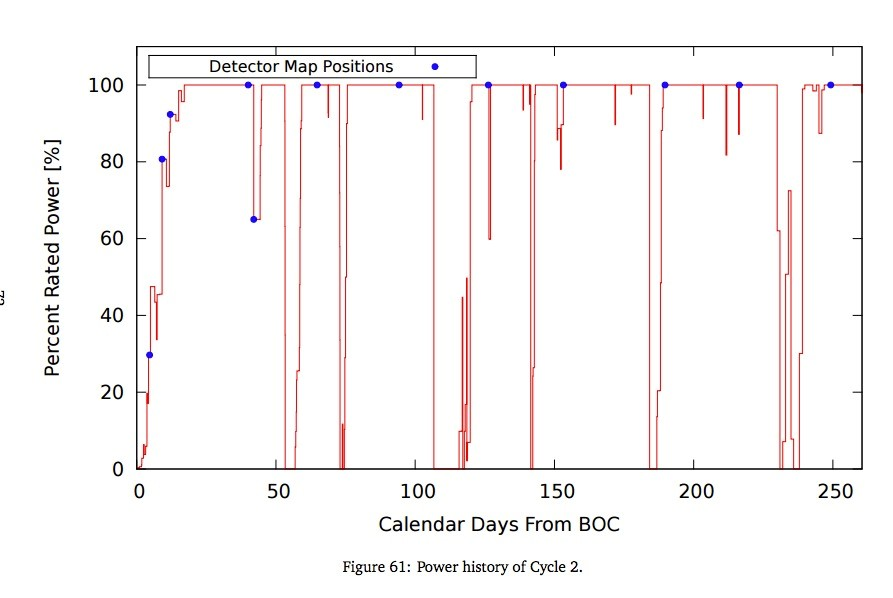
\includegraphics[width = 4.5 in]{figures/cyc2_pow_his_old}
\caption{Cycle 2 power history in BEAVRS ver. 2.0.1}
\label{fig:cyc2powhist}
\end{figure}

The previous plot was missing the correct End Of Cycle point, at 296 calendar days since BOC, or 10.43 MWd/kg burnup. Figure \ref{fig:cyc2powhist_new} shows the correct plot and is included in version 2.0.2. Having a complete power history for both cycles is especially important in determining uncertainty through time series analysis, since only full power points will be considered in the analysis, and the Cycle 2 EOC burnup that has been omitted thus far is contained within the subset of full power points. The latest UQ work as well as all other work from this project will be compiled together in the final release, BEAVRS v3.0, in the future.

\begin{figure}[!htb]
\centering
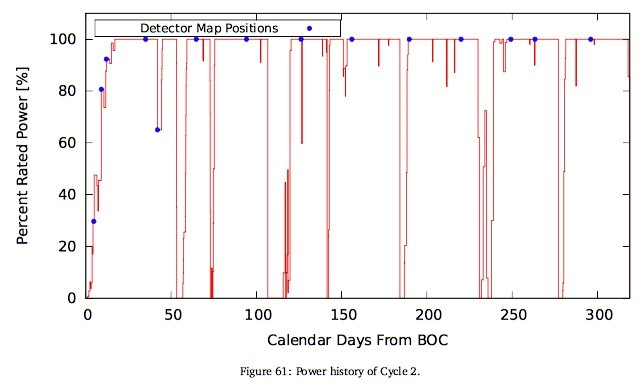
\includegraphics[width = 4.5 in]{figures/cyc2_pow_his_new}
\caption{Updated cycle 2 power history in BEAVRS ver. 2.0.2}
\label{fig:cyc2powhist_new}
\end{figure}



\subsection{BEAVRS Specifications - Version 2.0.1}
BEAVRS v2.0 was released in September 6th, 2016. This release included a few improvements on the BEAVRS model as well as newly added data, for example, the inlet coolant temperature measurements. The densities of materials in the nozzle and support plate regions are changed to preserve the mass of steel and volume fraction of water when assuming a simplified geometry for the nozzles and support plate components. Also added was eighth-core symmetric radial data, or tilt-corrected radial data, which is generated by adjusting the detector measurements to correct the planar x-y tilt.

Version 2.0.1 of the BEAVRS specification contains several more updates according to feedback obtained from the benchmark users. For instance, CASL users reported some detector measured axial signals are not correctly lined up when they were validating the VERA code. A more accurate and robust algorithm was then implemented to re-align the signals.

Detailed changes include:
\begin{itemize}
\item Slight shifts to all axial planes
\item Added B4C control rod material and updated the control rod specification
\item Updated the grid spacer specifications with more accurate heights
\item Updated the control rod 0\% withdrawn axial location
\item Updated the burnable poison insertion axial location
\item Added upper plenum and end plugs to burnable poison rods
\item Added upper plenum, end plugs, and spacer region to control rods
\item Changed from air to helium for control rod and control rod gaps
\item Updated neutron shield panel specification
\item Updated RPV geometry and material specification
\item Added the core liner
\item Added water gap between fuel assemblies and baffle
\item Added new materials for nozzle and support plate structure to conserve mass and volume fractions
\item Added inlet coolant temperature measurements
\item Added tilt-corrected data
\item Re-calculated all material compositions using latest isotopic natural abundances data, IUPAC 2013
\item Corrected the critical Boron concentration from 1237 to 1273 ppm in Cycle 2
\item Improved re-alignment algorithm in processing measurement data
\end{itemize}

The updates in the core structure are summarized in the figures below.

\begin{figure}[ht]
\centering
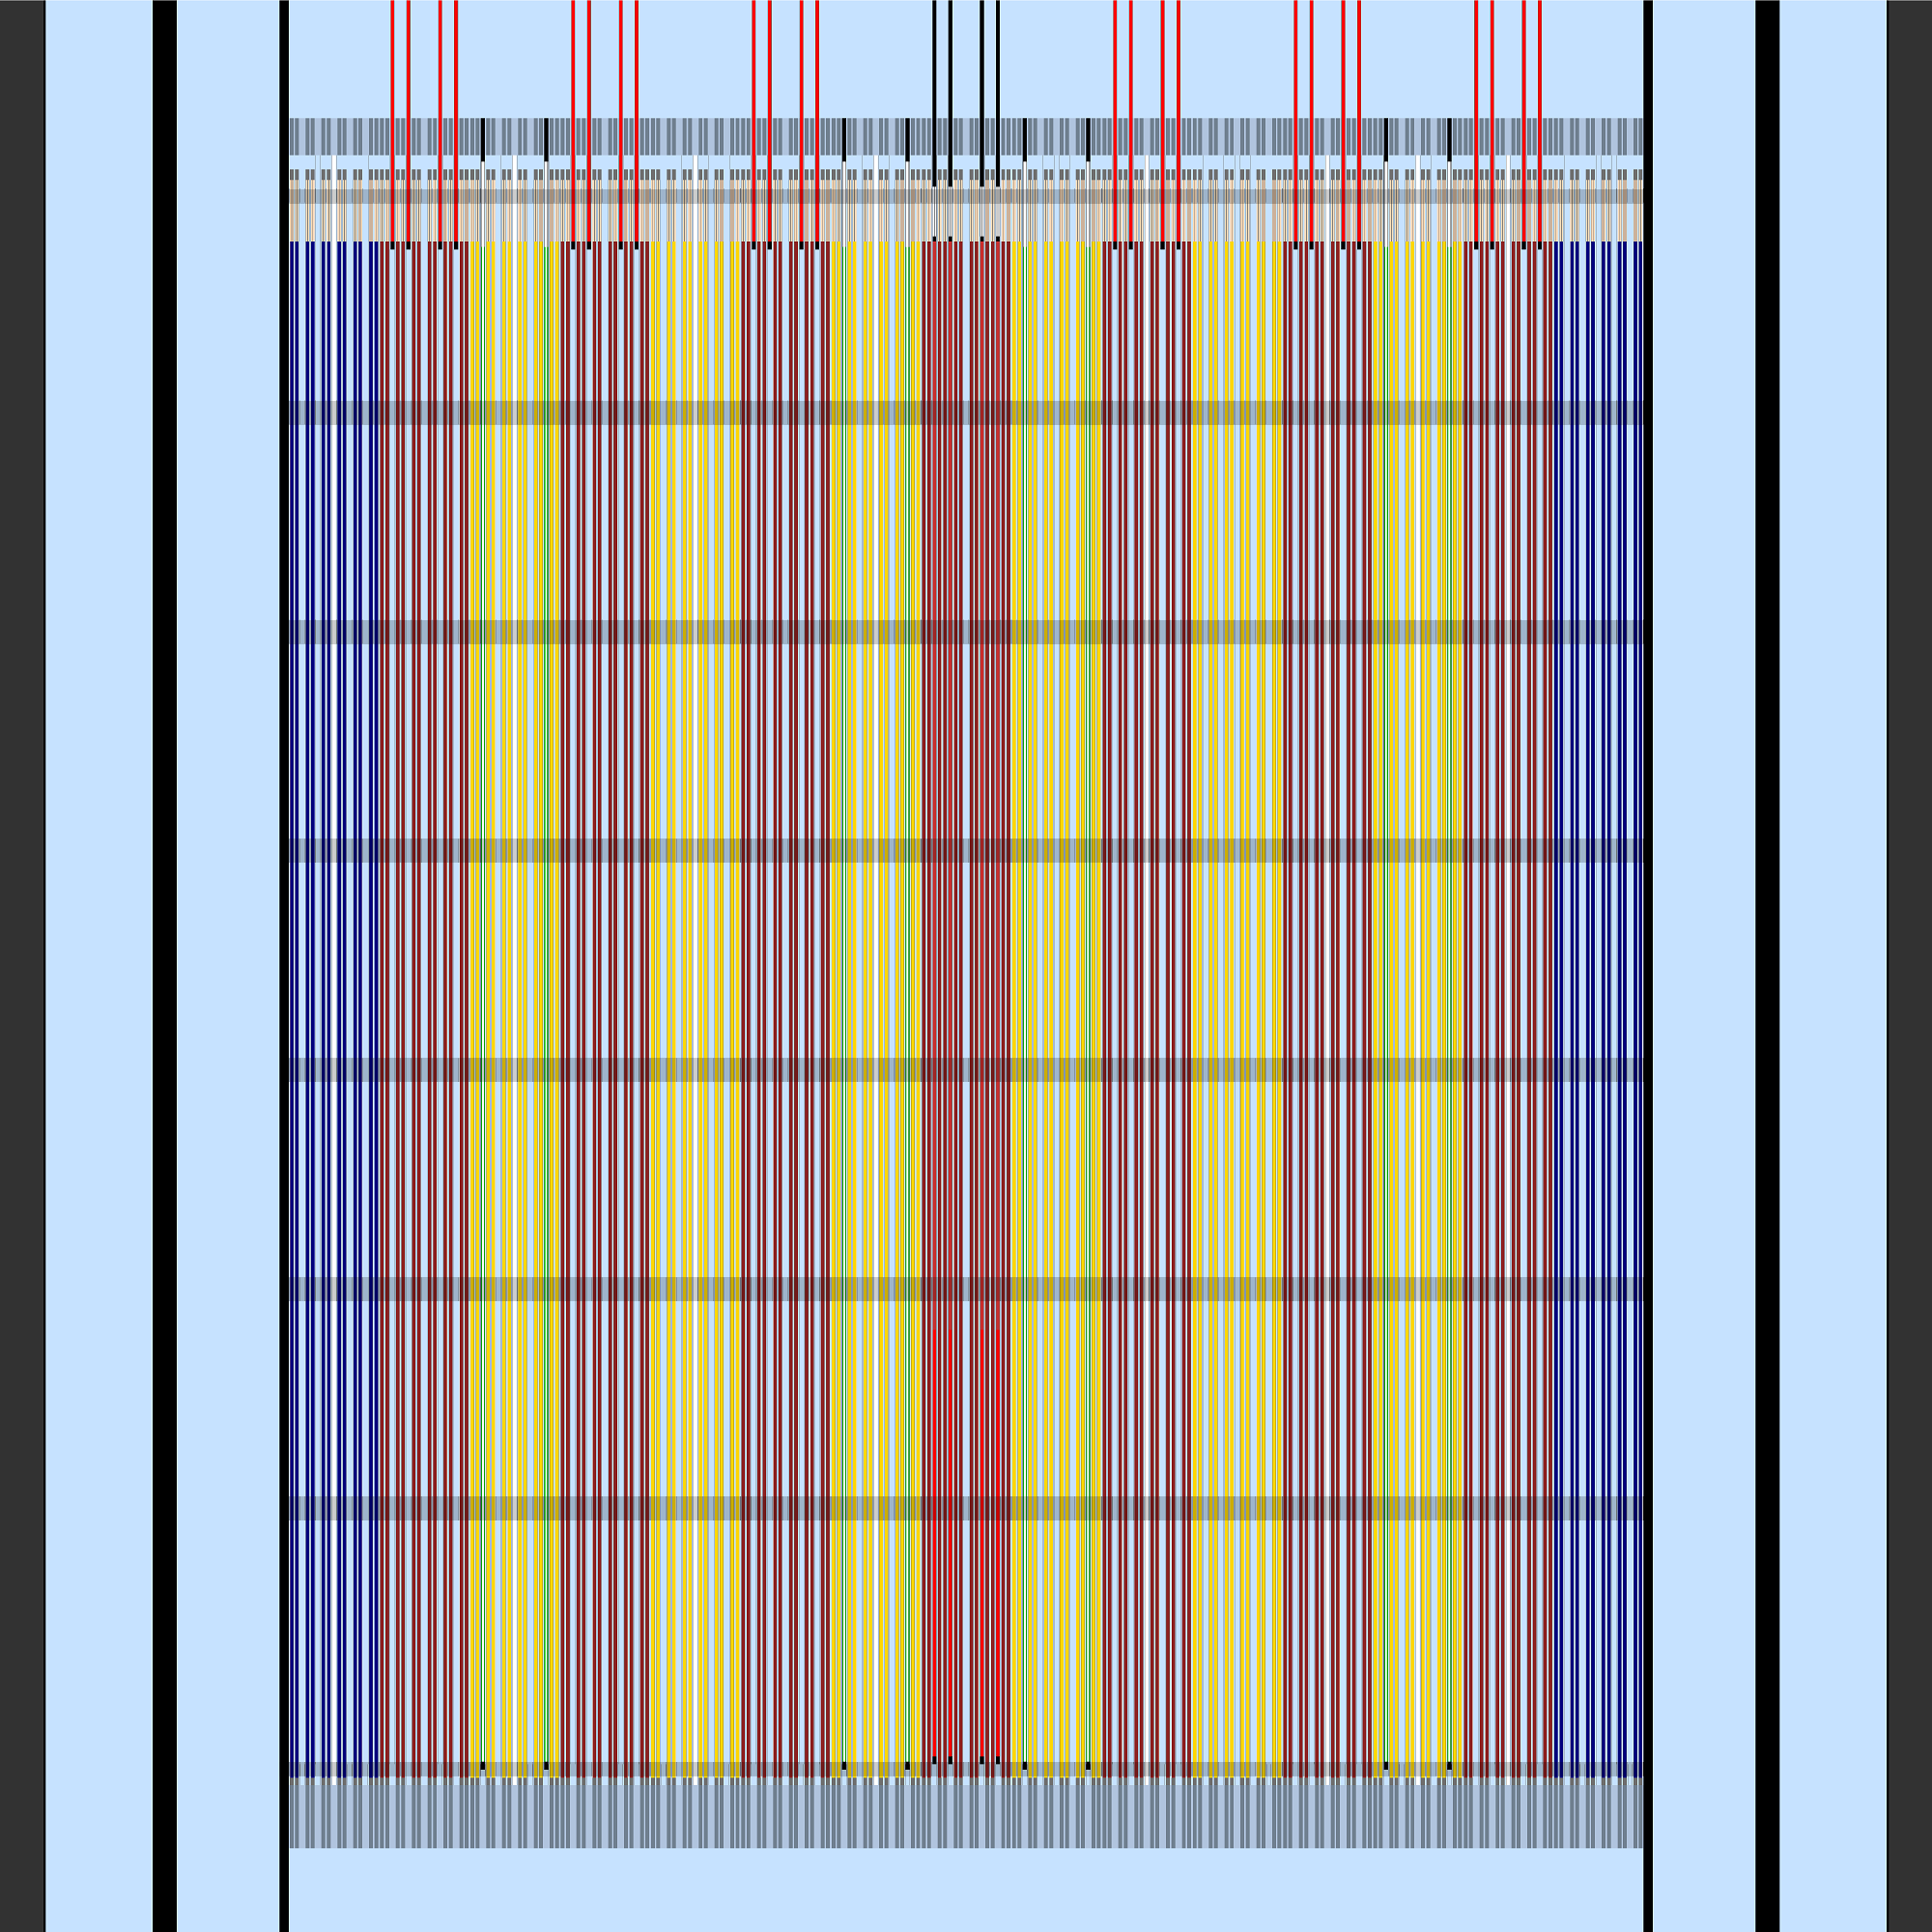
\includegraphics[keepaspectratio, width = 4.5 in]{figures/row_8_mats_axial_grids_enhanced}
\caption{Scale view of row 8 axial cross section, with highlighted grid spacers and partial insertion of control rod bank D to the bite position}
\label{fig:axial_row_8}
\end{figure}
\FloatBarrier 

\begin{figure}[ht]
\centering
\centering
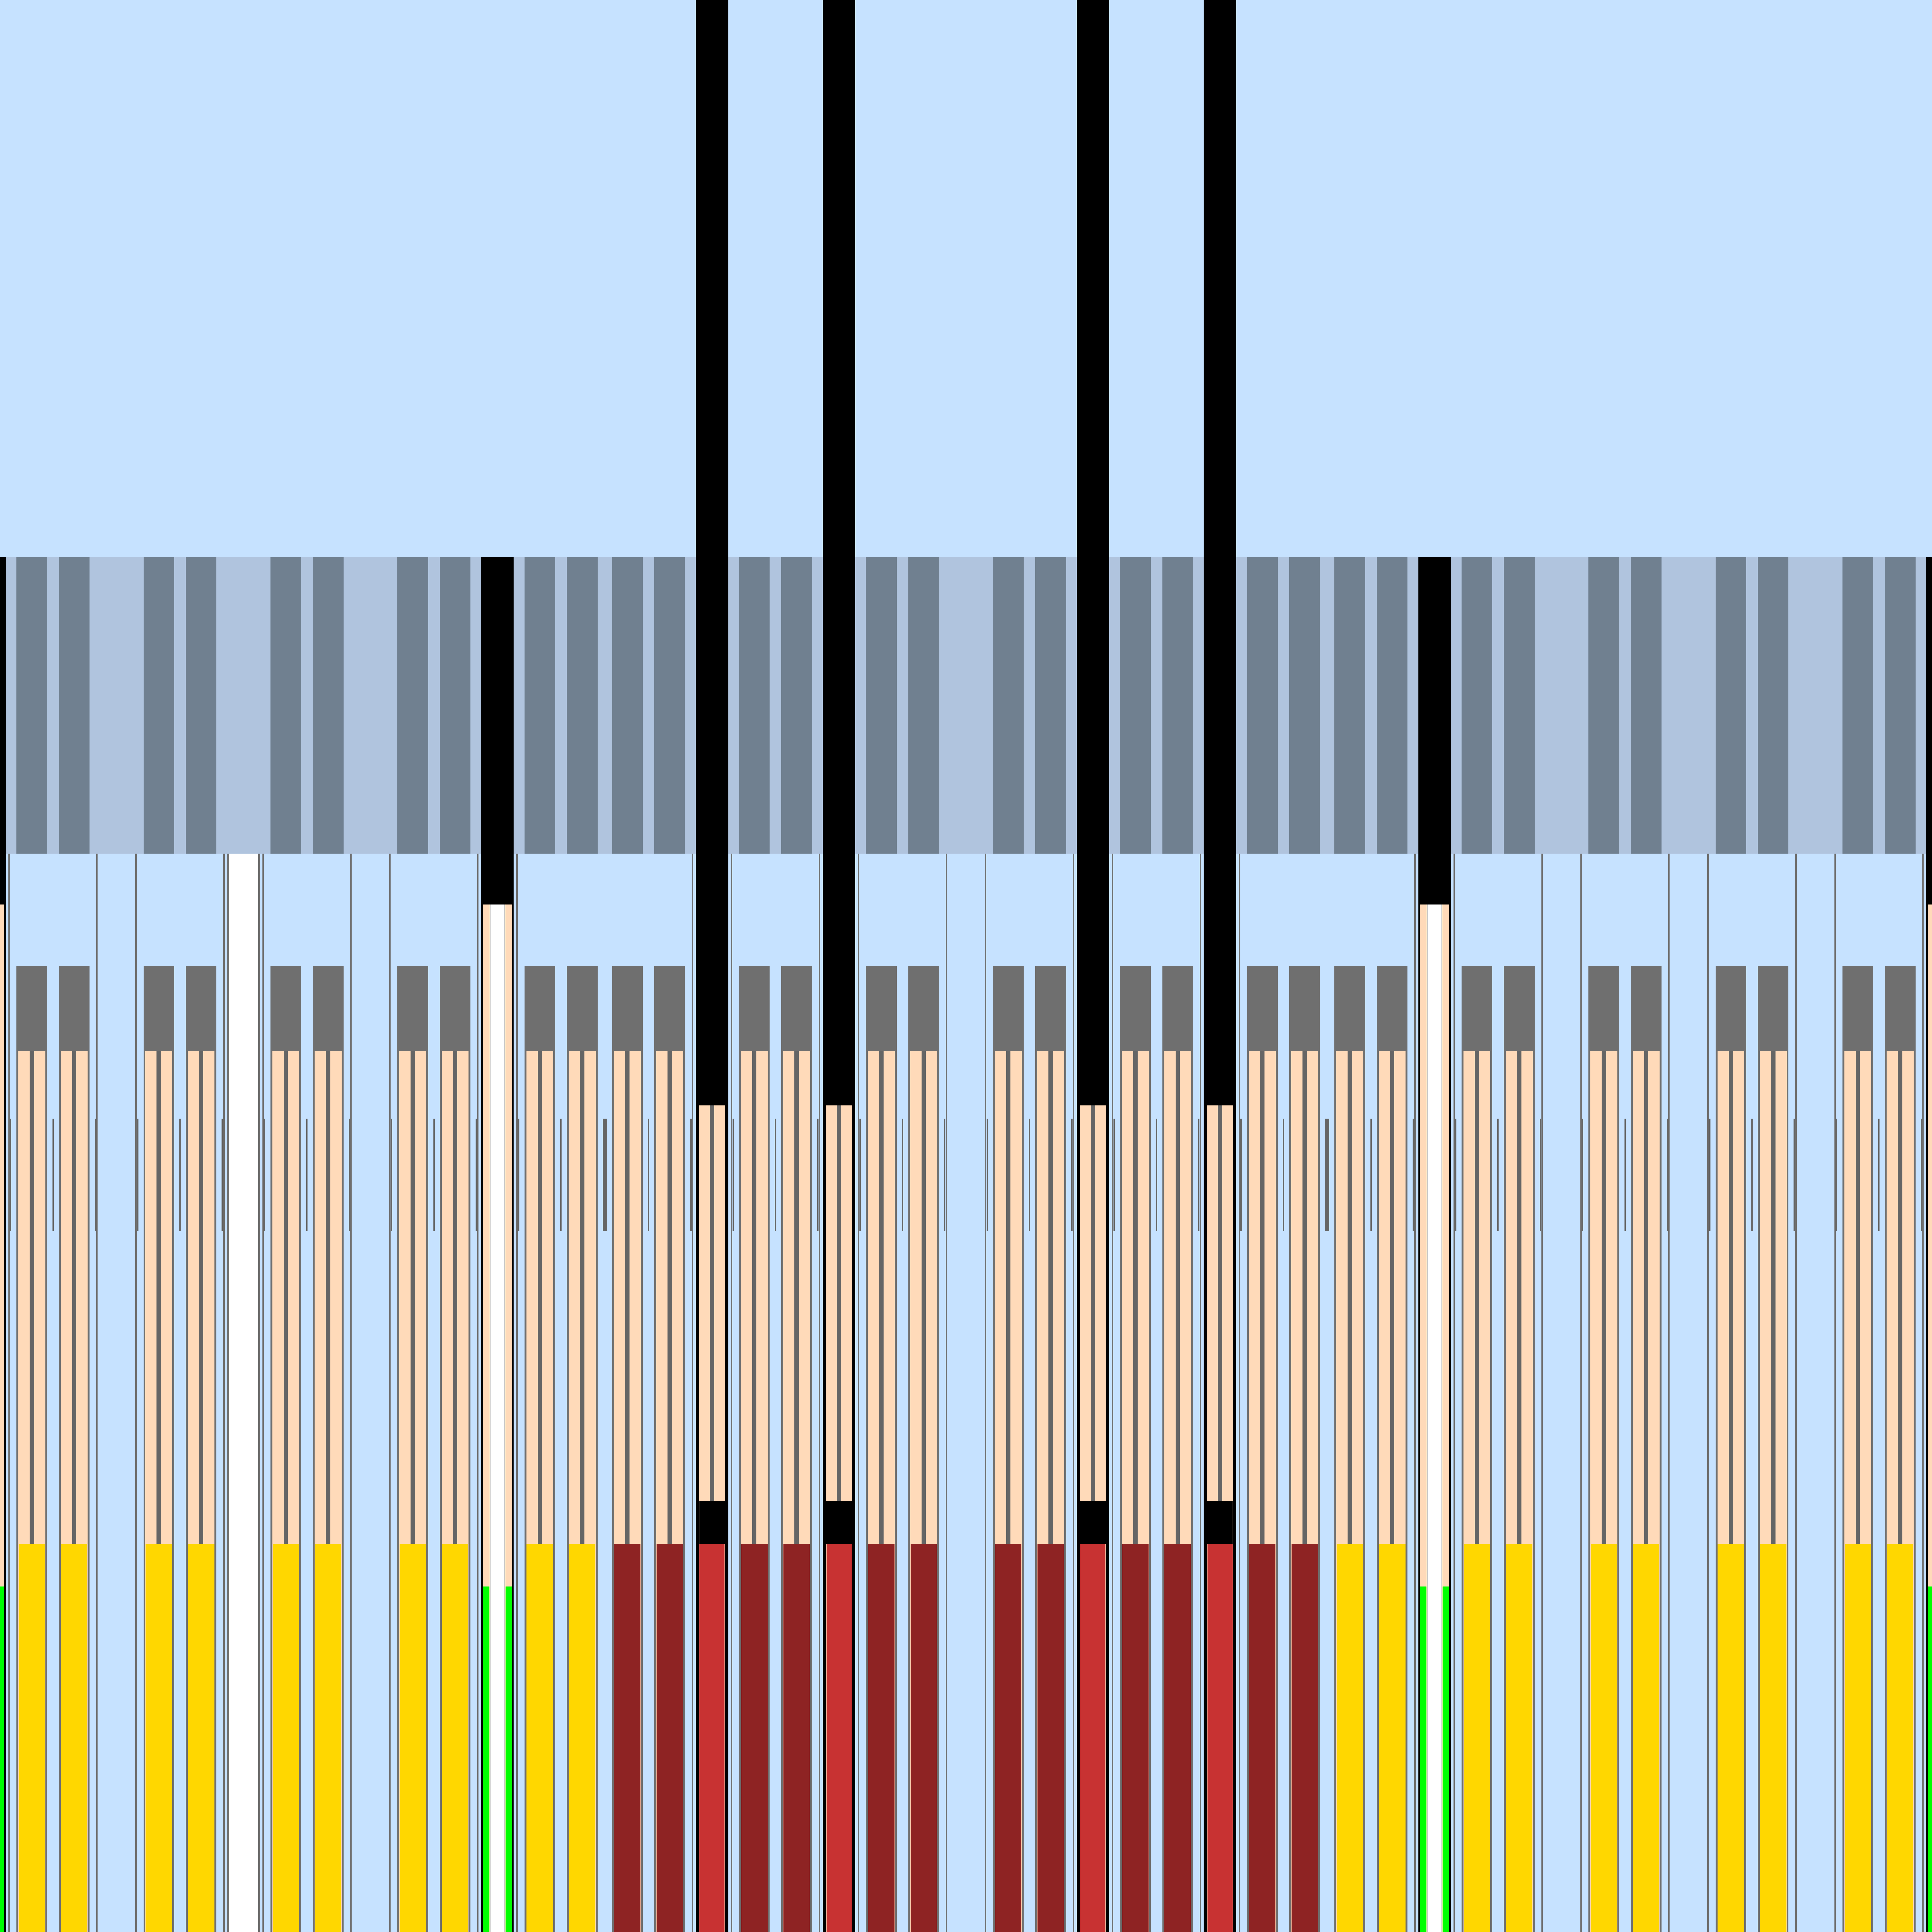
\includegraphics[keepaspectratio, width = 2.5 in]{figures/axial_mats_row_8_topzoom}
\caption{Axial scale view of the model near the top of the fuel rods in row 8, show pin plenums, approximated springs, end plugs, and structures.  \emph{Blue}: water; \emph{orange}: helium;  \emph{black}: stainless steel; \emph{dark gray}: Zircaloy; \emph{dim gray}: Inconel; \emph{white}: air; \emph{slate gray}: nozzle / support plate stainless steel; \emph{steel blue}: nozzle / support plate borated water; \emph{green}: borosilicate glass; \emph{yellow}: fuel.}
\label{fig:top_core_zoom}
\end{figure}

\begin{figure}[ht]
\centering
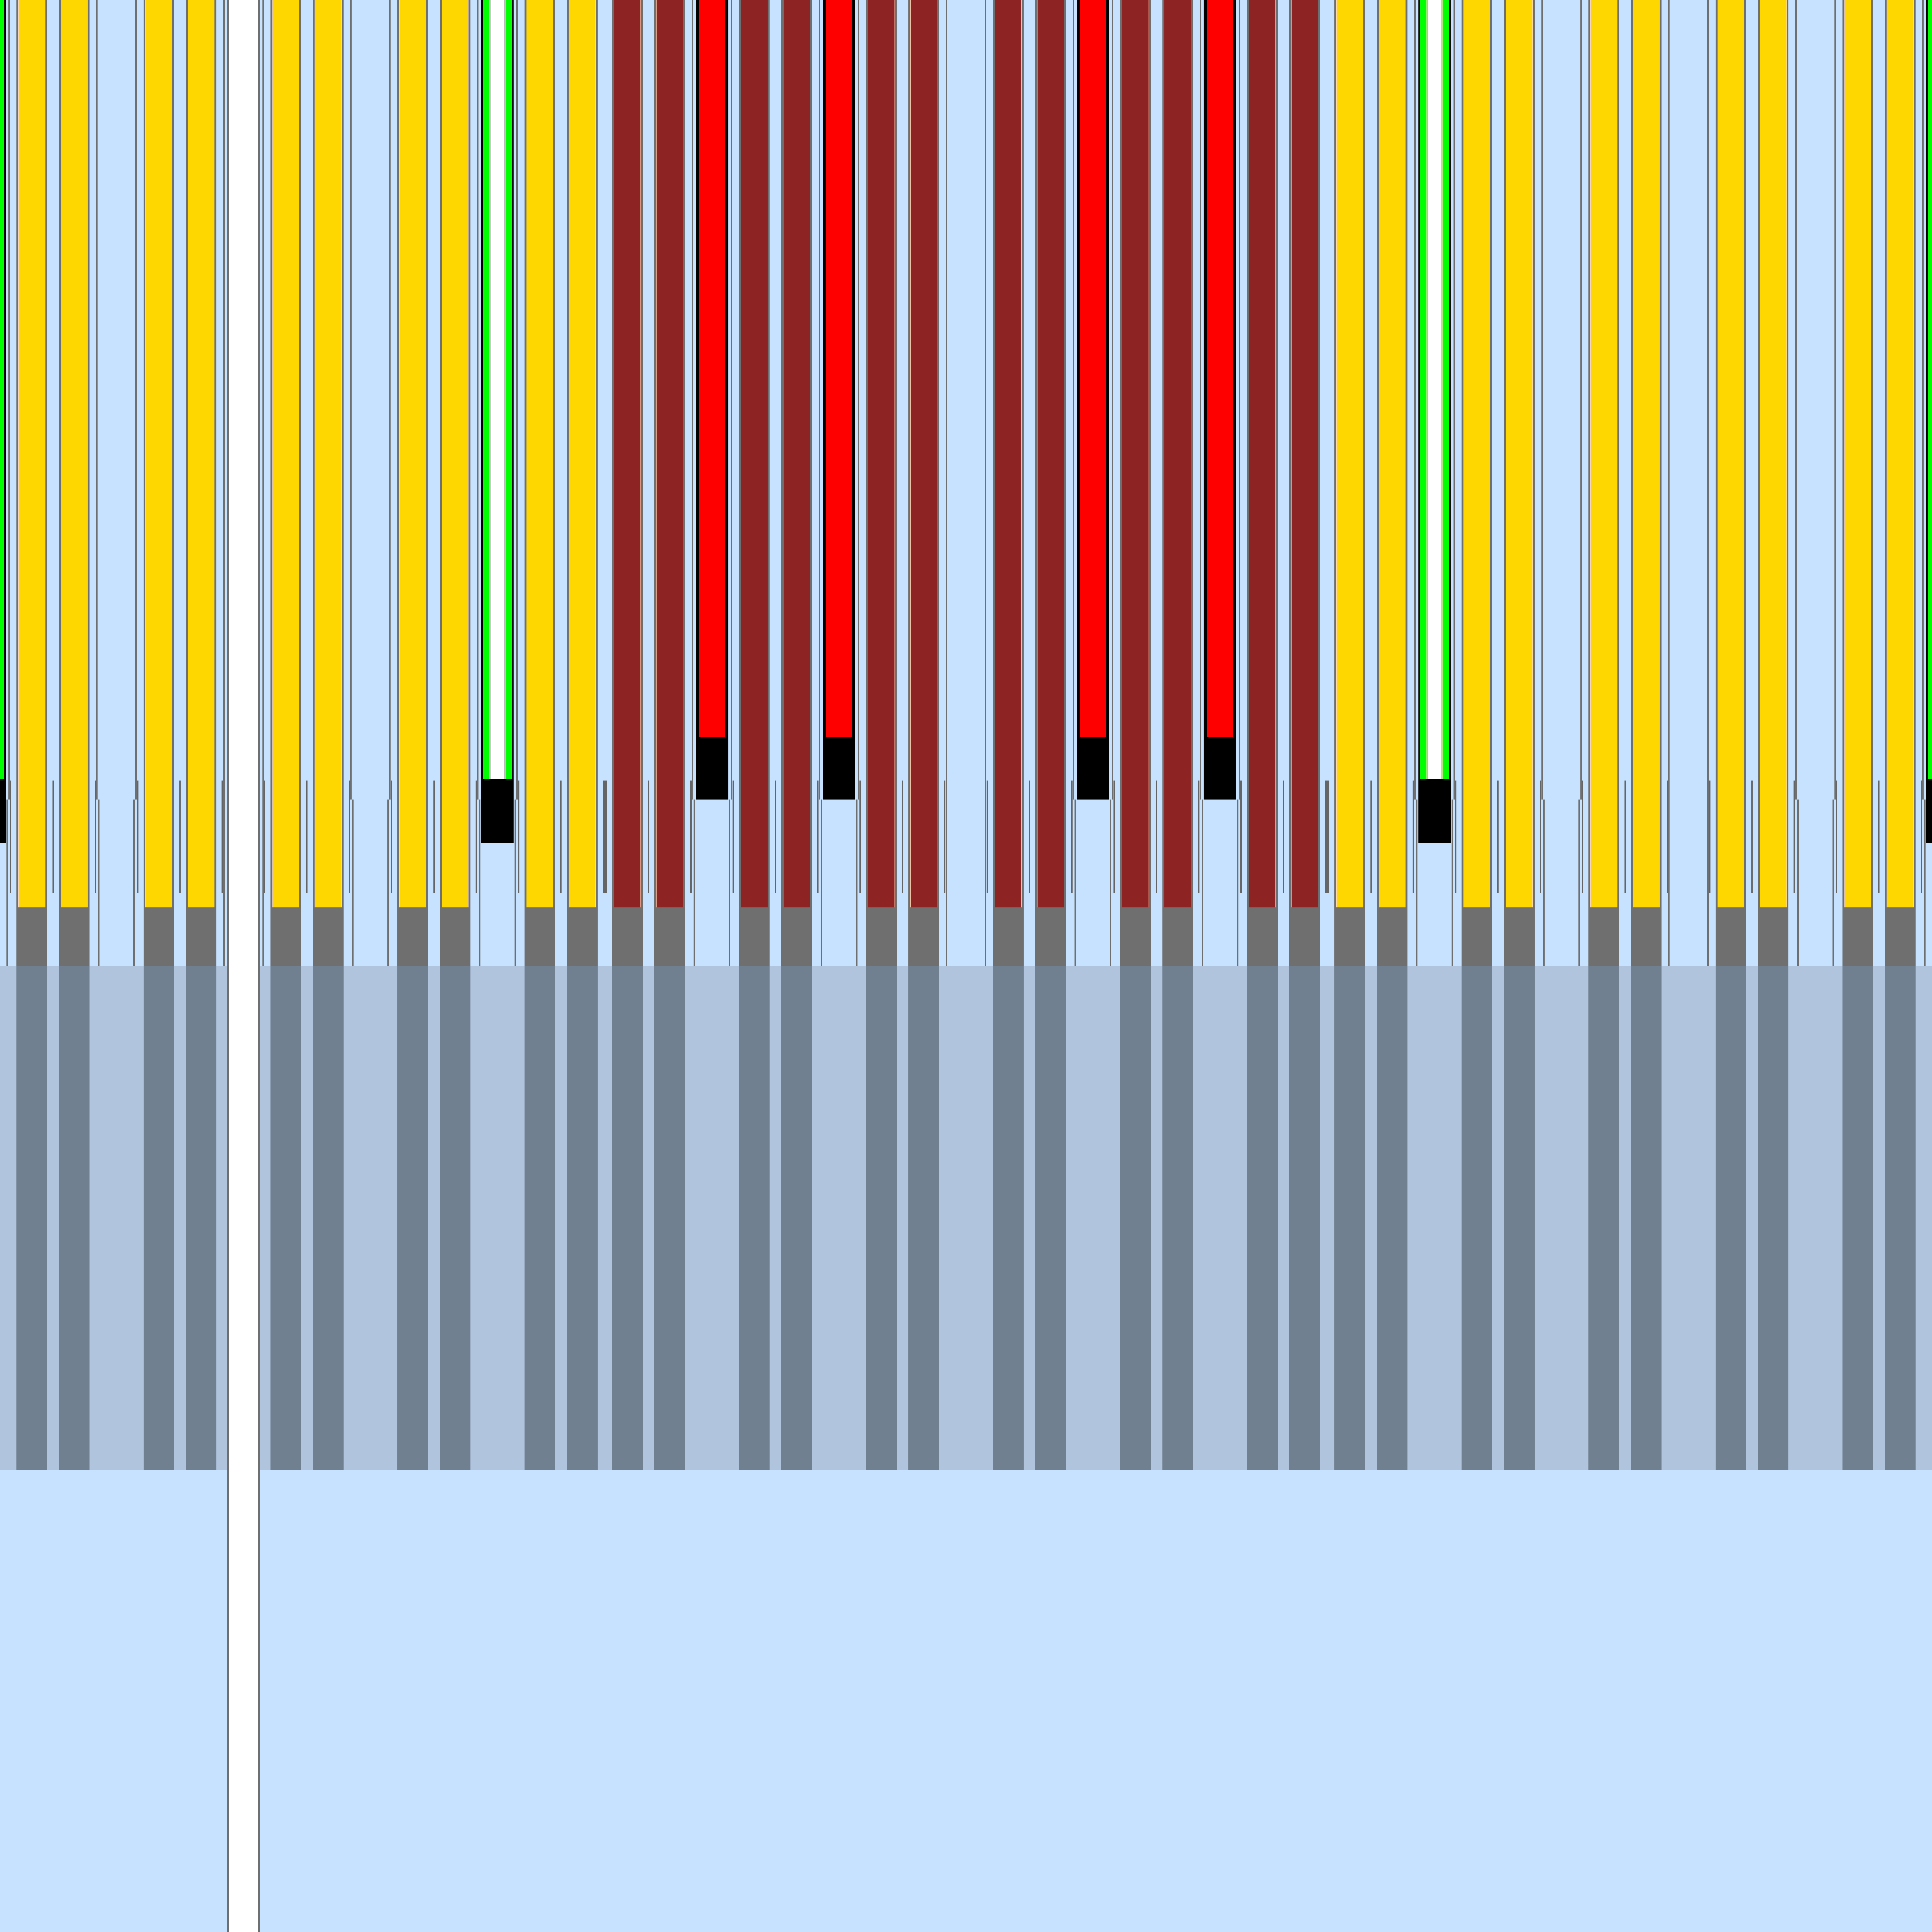
\includegraphics[keepaspectratio, width = 2.5 in]{figures/axial_mats_row_8_botzoom}
\caption{Axial scale view of the model near the bottom of the fuel rods in row 8, show pin plenums, approximated springs, end plugs, and structures. \emph{Blue}: water; \emph{orange}: helium;  \emph{black}: stainless steel; \emph{dark gray}: Zircaloy; \emph{dim gray}: Inconel; \emph{white}: air; \emph{slate gray}: nozzle / support plate stainless steel; \emph{steel blue}: nozzle / support plate borated water; \emph{green}: borosilicate glass; \emph{yellow}: fuel.}
\label{fig:bot_core_zoom}
\end{figure}
\FloatBarrier

\begin{figure}[ht]
\centering

\includegraphics[keepaspectratio, width = 2.5 in]{figures/J8_nozzle}
\caption{Radial picture of nozzles and support plate. The materials below and above the fuel rod regions are defined as "nozzle / support plate stainless steel" in color \emph{slate gray} and "nozzle / support plate borated water" in color \emph{steel blue} to conserve the mass the stainless steel and borated water in the nozzle and support plate region.}
\label{fig:nozzle}
\end{figure}
\FloatBarrier


\subsection{Benchmark Submission}

This benchmark is proposed for inclusion in the international handbook, International Reactor Physics Experiment Evaluation Project (IRPhEP) of OECD/NEA. An initial version of the BEAVRS evaluation, identified as “BEAVRS-PWR-POWER-001 CRIT-REAC-COEF-RRATE”, was submitted to the IRPhEP Technical Review Group in September. We were invited to attend the IRPhEP Technical Review Meeting 2017 in October 24-26 in Washington, DC. The submitted BEAVRS benchmark was presented and reviewed. The benchmark will be included in the handbook once all comments are addressed.

The IRPhEP submission for BEAVRS was prepared based on existing BEAVRS documents. The previous specifications were re-formatted in the required Word format. Four types of measurements, critical configuration, reactivity effect measurements, reactivity coefficient measurements and reaction rate distribution measurements were presented.  Also compiled was the uncertainty quantification analysis of all measurements. New computer codes simulations were incorporated as well, including OpenMC and CASMO/Simulate inputs and results.

\section{Task: HZP Measurement Uncertainties}

\subsection{Assembly loading}

As built assembly enrichment and loaded position are known for every assembly in the first 2 cycles of the BEAVRS benchmark. For modelling purposes it is simpler to consider only 3 different loading enrichment instead of 193 unique ones.  The following tables summarize the average enrichment for each batch and standard deviation for the first two cycles.

\begin{center}
\begin{tabular}{ l c c c }
\hline
  & Fuel 1.6\% & Fuel 2.4\% & Fuel 3.1\% \\
\hline  
  Number of assemblies & 65 & 64 & 64\\
  Average enrichment & 1.610 & 2.400 & 3.102 \\
  Standard deviation & 0.004 & 0.005 & 0.014 \\
\hline  
\end{tabular}
\end{center}

\begin{figure}
\centering
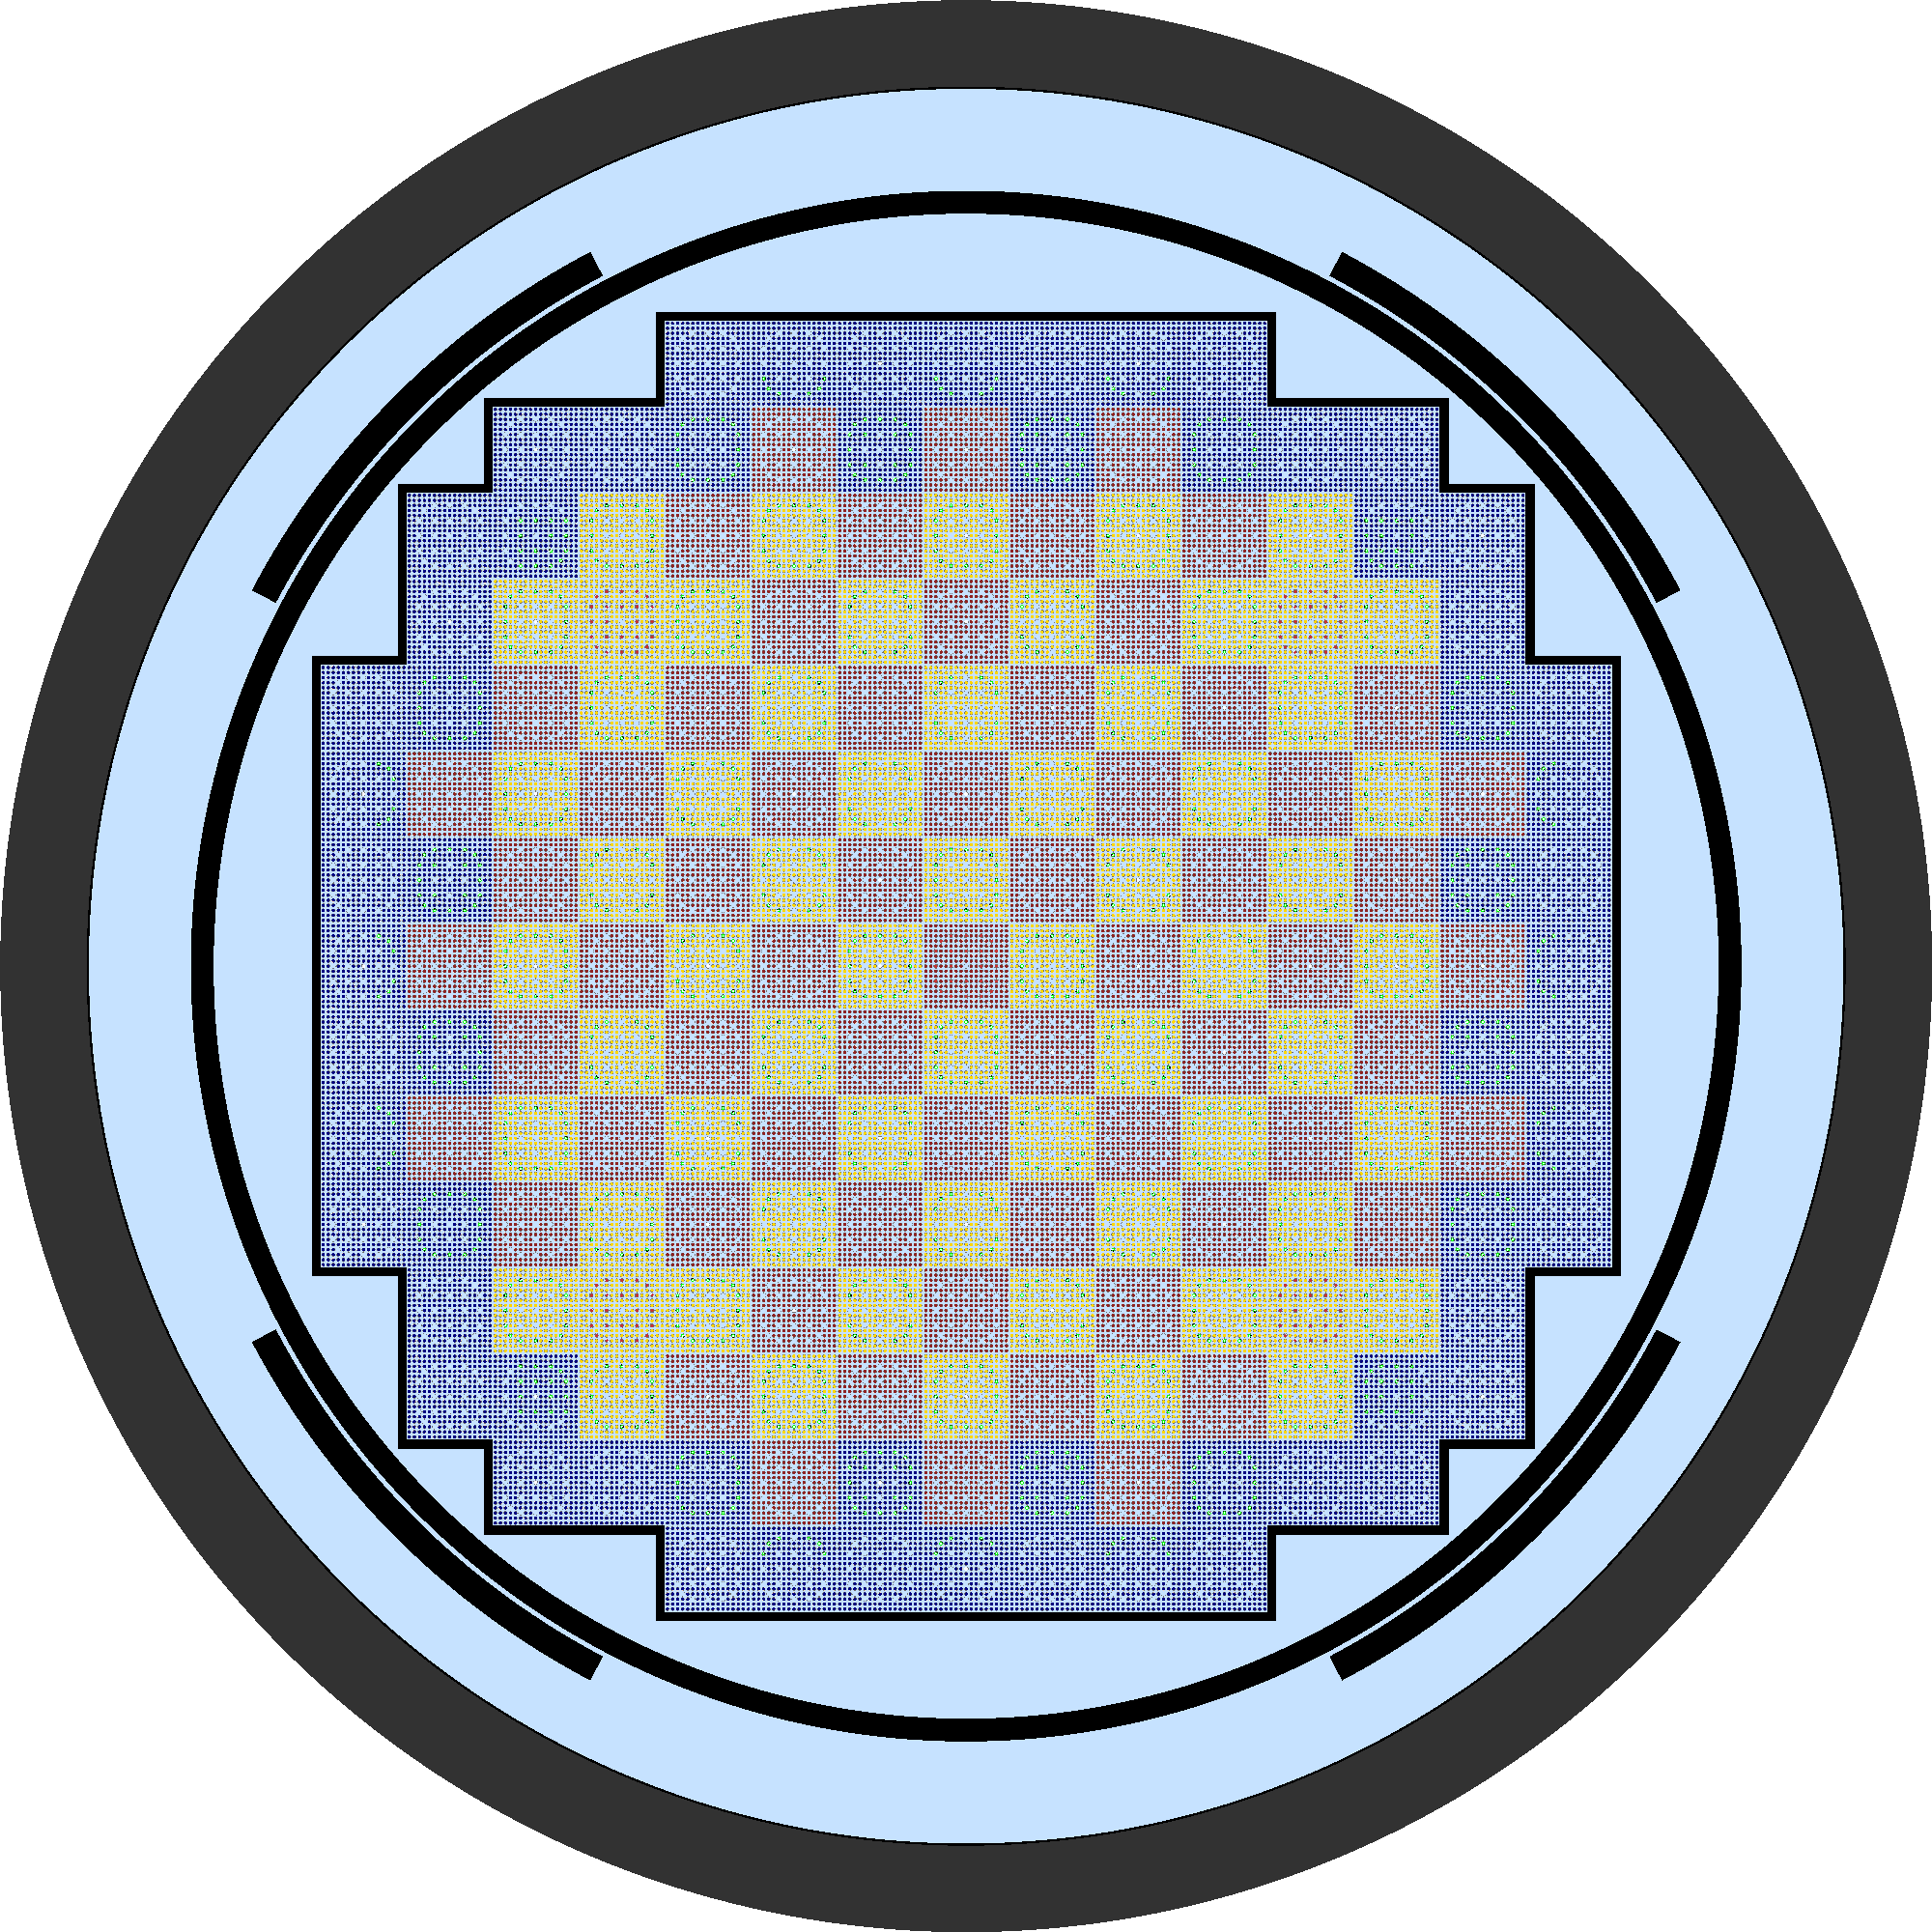
\includegraphics[keepaspectratio, width = 4.0 in]{figures/pwr_core.png}
\caption{Cycle 1 core loading}
\label{fig:cycle1_map}
\end{figure}

\begin{center}
\begin{tabular}{ l c c}
\hline
  & Fuel 3.2\% & Fuel 3.4\% \\
\hline  
  Number of assemblies & 48 & 16\\
  Average enrichment & 3.195 & 3.406 \\
  Standard deviation & 0.005 & 0.003 \\
\hline  
\end{tabular}
\end{center}

\subsection{Low Power Physics Tests}

This report discusses the estimated uncertainties for the BEAVRS benchmark on the hot zero power (HZP) physics tests.  Since the BEAVRS measurements were performed a long time ago and very little data exists that can be used to evaluate the uncertainties, more recent data using similar techniques will be used to assess a best estimate of uncertainty to the BEAVRS data.  This data set was provided by KHNP who started 4 OPR reactors with nominally identical cores.  This data will be used to evaluate the uncertainties associated with measurements of critical boron concentration, isothermal temperature coefficients and control rod worths.  Obviously the OPR reactors are different to the BEAVRS model, but this modern data will still be used as the basis for measurement uncertainty since the measurement techniques are comparable.  When possible, comparisons with other literature data points will be made to support this analysis.  It should also be noted that many of the HZP measurements rely on the reactivity computer settings.

\subsubsection{Critical Boron Concentration}

In the OPR reactors, the critical boron concentration (CBC) was measured under three scenarios:
\begin{enumerate}
\item All rods out (ARO)
\item Shutdown bank B (SDB) in
\item Regulating group 1 (RG1) in
\end{enumerate}

The process for measurement can be summarized as follows:
\begin{enumerate}
\item Borate the reactor coolant system (RCS) to withdraw all rods (for ARO case) except for regulating group 5 (RG5)
\item Withdraw RG5 partially and record position
\item Withdraw RG5 to upper limit and record reactivity ($\Delta RG5$)
\item Measure boron concentration ($C_M$)
\item Calculate $CBC$ using inverse boron worth ($IBW$)
\begin{equation}
  CBC = C_M + \frac{\Delta RG5}{IBW}
\end{equation}
\end{enumerate}

Looking at the measurement data from the 4 nominally identical OPR reactors, the measurement reproducibility is on the order of 8 ppm.  However, this value does not include any uncertainties associated to the IBW obtained from simulation and uncertainties from the reactivity computer and its underlying parameters and assumptions.  Thus the 8 ppm uncertainty can be attributed to the critical boron concentration measurement, but we must still account for the rod worth differential and the IBW.  From the provided data, we can propagate the uncertainty of these parameters using the following relation:
\begin{equation}
  \delta CBC = \sqrt{\left( \frac{\partial CBC}{\partial C_M} \delta C_M \right)^2 + \left( \frac{\partial CBC}{\partial \Delta RG5} \delta \Delta RG5 \right)^2 + \left( \frac{\partial CBC}{\partial BW} \delta BW \right)^2}
\end{equation}
which yields
\begin{equation}
  \delta CBC = \sqrt{\left( \delta C_M \right)^2 + \left( BW \delta \Delta RG5 \right)^2 + \left( \Delta RG5 \delta BW \right)^2}
\end{equation}
The last term is quite small and can be neglected. We also know the boron worth ($BW$) from measurement.  Assuming that the repeated measurements provide an estimate for $C_M$ of 8 ppm, this leaves determining the reactivity change error associated with small movements of $RG5$.  This error is associated with knowing the position of the rod and its associated reactivity effect for a small change, and not the measurement error of the reactivity worth when fully withdrawn.  Since the rod movement of RG5 is limited to approximately one tenth of its length, and assuming a measurement uncertainty of less than 5\% (see control rod worth section), we can estimate the critical boron concentration uncertainty to be 22 ppm.

In the literature, a recent paper performing full core analysis of the Krsko plant reported critical boron measurement uncertainties of 20 ppm.  This value is in line with the calculated value from the OPR data.  Both values are also well below the common licensing criterion of 50 ppm for prediction from models.

\begin{table}[ht]
\centering
\caption{BEAVRS Cycle 1 Critical Boron Concentrations}
\begin{tabular}{ |c|c|c| } 
 \hline
 Case & Critical Boron (ppm) & Std. Dev. (ppm) \\  
 \hline
 ARO & 975 & 22 \\ 
 D in & 902 & 22  \\
 C,D in & 810 & 22  \\
 A,B,C,D in & 686 & 22  \\
 A,B,C,D,SE,SD,SC in & 508 & 22  \\
 \hline
 \end{tabular}
\label{tab:cyc1_boron_conc}
\end{table}

\begin{table}[ht]
\centering
\caption{BEAVRS Cycle 2 Critical Boron Concentrations}
\begin{tabular}{ |c|c|c| } 
 \hline
 Case & Critical Boron (ppm) & Std. Dev. (ppm) \\  
 \hline
 ARO & 1405 & 22 \\ 
 C in & 1237 & 22  \\
 \hline
 \end{tabular}
\label{tab:cyc2_boron_conc}
\end{table}

\subsubsection{Isothermal Temperature Coefficient}

The isothermal temperature coefficient (ITC) test is performed using the following procedure:
\begin{enumerate}
\item Decrease temperature at a rate of 5 to 10 K per hour using the steam bypass control system
\item Maintain at 5 C below until data is recorded
\item Increase temperature at a rate of 5 to 10 K per hour using the steam bypass control system
\item Maintain at 5 C above until data is recorded
\item Return to temperature
\item Calculate RTC using changed in reactivity and reactor control system temperature for each change in temperature, and average results
\end{enumerate}

In this procedure the ITC is thus measured 3 times and averaged.  Only the average value is reported with its associated uncertainty.  The OPR data contains 2 sets of measurements for all 4 reactors; one with all rods out (ARO) and one with shutdown bank B (SDB) fully inserted. For these cases, the ITC reported deviation is roughly 0.2 pcm/K.

The Palo Verde report \cite{paloverde} presents ITC measurements at cycle 1 for their three nominally identical cores.  Using their data, the deviation is on the order of 0.6 pcm/K. In a recent paper, the analysis performed on the Krsko NPP reports ITC measurement errors of 1.8 pcm/K.  There thus exists very little agreement between the published literature and the measurements obtained from KHNP.  The value from the Krsko plant seems unusually high and provides no supporting documentation.  We thus have 11 measurements separated over three data sets.  Weighing them by the number of data points in each set, we can approximate the ITC uncertainty to 0.3 pcm/K or 0.54 pcm/F.

\begin{table}[ht]
\centering
\caption{Palo Verde ITC data for Cycle 1 of all three units}
\begin{tabular}{ |c|c| } 
 \hline
 Unit & ITC (pcm/F) \\  
 \hline
 1 & -4.40 \\ 
 2 & -4.28 \\
 3 & -3.79 \\
 \hline
 \end{tabular}
\label{tab:palov_itc_cyc1}
\end{table}


\begin{table}[ht]
\centering
\caption{BEAVRS Cycle 1 ITC}
\begin{tabular}{ |c|c|c| } 
 \hline
 Case & ITC (pcm/F) & Std. Dev. (pcm/F) \\  
 \hline
 ARO & -1.75 & 0.54 \\ 
 D in & -2.75 & 0.54  \\
 C,D in & -8.01 & 0.54  \\
 \hline
 \end{tabular}
\label{tab:beavrs_itc_cyc1}
\end{table}

\begin{table}[ht]
\centering
\caption{BEAVRS Cycle 2 ITC}
\begin{tabular}{ |c|c|c| } 
 \hline
 Case & ITC (pcm/F) & Std. Dev. (pcm/F) \\  
 \hline
 ARO & -1.71 & 0.54 \\ 
 \hline
 \end{tabular}
\label{tab:beavrs_itc_cyc2}
\end{table}


\subsection{Control Rod Worth}

At the time the BEAVRS reactor was started the most common way to measure control rod worths was with boron dilution followed by rod swap.  Some of the early cores were done entirely by boron dilution, but to accelerate startup time, the rod swap technique became quite common once rod worth for one bank was known.  

The boron dilution technique involves a decrease in boron concentration following a rod insertion in a sequence of small discrete steps.  The reactivity computer print out is then used to calculate the incremental reactivity changes at each insertion.  This method is very precised but very time consuming since sufficient wait time must be allowed during insertions for flux stabilization.

The rod swap technique requires that at least one bank be computed using the dilution technique to serve as a reference.  The reference bank is often selected to be the highest worth bank since less rod displacement will be required.  In this technique, the bank to be evaluated is compensated by the reference bank.  The differential is then measured to calculate the effective reactivity with respect to the reference.

In the OPR reactors, the boron dilution technique is used for SDB and RG1, while rod swap is used for all others. Standard deviations were calculated for each rod bank and converted into relative error (standard deviation divided by average).  Additionally, since the cores are not entirely the same, predicted rod worths were used to include deviations in as-built fuel enrichment.  However, correcting the experimentally measured values by the predicted ones, barely changed the uncertainty indicating that the measurement errors are much larger than the enrichment differences.

Figure \ref{fig:fig_trend_line} shows the trend line obtained from the data and the fitting function.  Actual data points were omitted due to the proprietary nature of the data from KHNP.  The red line indicates the plant acceptance criteria for deviations between the predictive models and measurements.


\begin{figure}[ht]
   \centering
   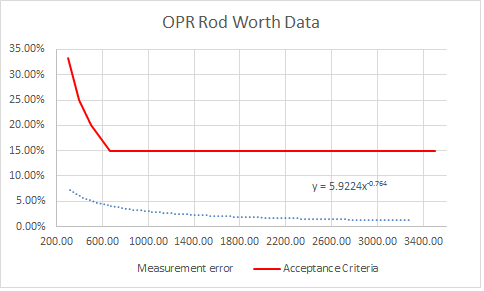
\includegraphics[keepaspectratio, width = 4.0 in]{figures/rod_worth.png}
   \caption{Trend line of rod worth measurement errors}  
   \label{fig:fig_trend_line}
 \end{figure} 
 
Using this data with the BEAVRS reported rod worths provides an estimate of the measurement errors as shown in Table \ref{tab:cycle1} and Table \ref{tab:cycle2}.

\begin{table}[ht]
\centering
\caption{BEAVRS Cycle 1 Rod Worths}
\begin{tabular}{ |c|c|c|c| } 
 \hline
 Bank & Rod Worth (pcm) & Error (\%) & Std. Dev. (pcm) \\  
 \hline
 D & 788 & 3.6 & 29 \\ 
 C & 1203 & 2.6 & 32 \\
 B & 1171 & 2.7 & 31 \\
 A & 548 & 4.8 & 26 \\
 SE & 461 & 5.5 & 25 \\
 SD & 772 & 3.7 & 28 \\
 SC & 1099 & 2.8 & 31 \\
 \hline
 \end{tabular}
\label{tab:cycle1}
\end{table}

\begin{table}[ht]
\centering
\caption{BEAVRS Cycle 2 Rod Worths}
\begin{tabular}{ |c|c|c|c| } 
 \hline
 Bank & Rod Worth (pcm) & Error (\%) & Std. Dev. (pcm) \\  
 \hline
 D & 426 & 5.8 & 25 \\ 
 C & 1014 & 3.0 & 30 \\
 B & 716 & 3.9 & 28 \\
 A & 420 & 5.9 & 25 \\
 SE & 438 & 5.7 & 25 \\
 SD & 305 & 7.5 & 23 \\
 SC & 307 & 7.5 & 23 \\
 SB & 781 & 3.6 & 29 \\
 SA & 326 & 7.1 & 23 \\
 \hline
 \end{tabular}
\label{tab:cycle2}
\end{table}

\section{Task: Flux Map Uncertainties}
\label{flux_map_unc}

This reactor contains 58 assemblies that can be accessed by in-core detectors, through the central guide tubes.  Figure \ref{fig:fig_instr_pos} shows these positions. There are six U-235 fission chambers with varying masses that are used to access the 58 positions. When measurements are being taken, multiple passes are performed to adequately measure all 58 assemblies. All detectors are passed through one common assembly for signal normalization. The detectors are inserted from the bottom until they reach the top and pulled back to measure the axial fission rate over 61 axial locations.

\begin{figure}[ht]
\centering
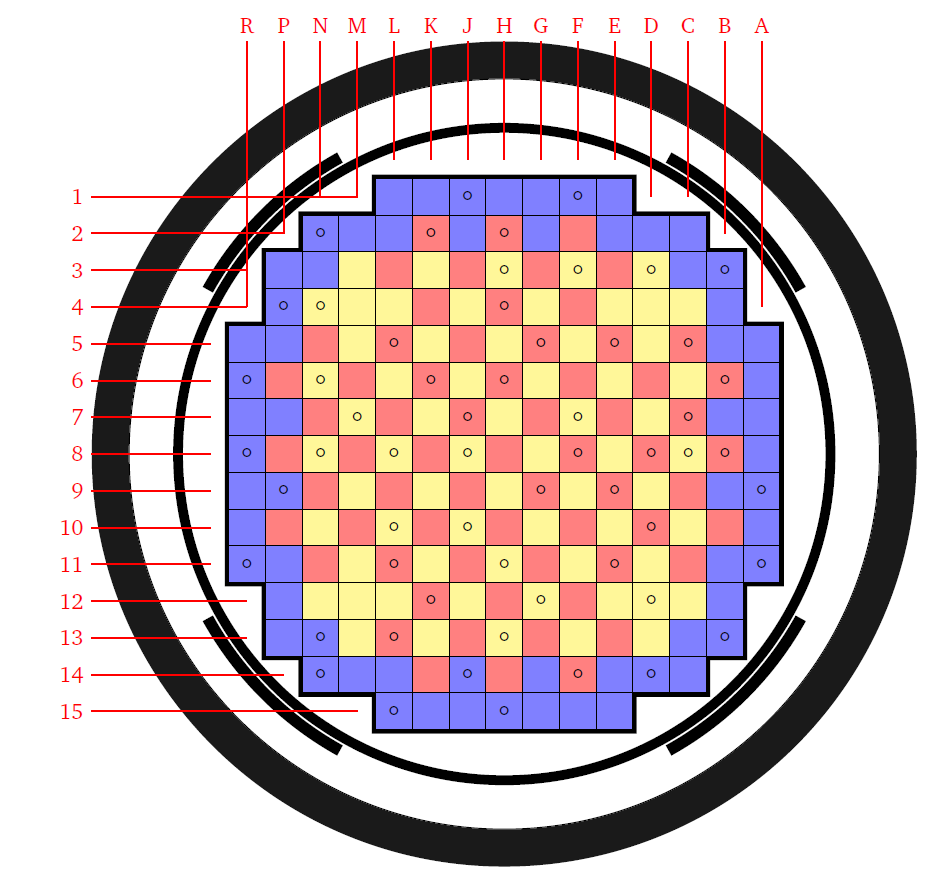
\includegraphics[keepaspectratio, width = 4.0 in]{figures/intrs_pos.png}
\caption{Instrument tube locations}
\label{fig:fig_instr_pos}
\end{figure}


\subsection{Extracting detector signals and processing data}

The raw measurement data for one detector in one pass includes 61 axial detector signals, background signal, gain factor of the detector and core power. The axial flux can be obtained from the detector signals by removing the background, adjusting the gain on the detector and dividing the power, as indicated in equation \ref{eq:detflux}.

\begin{equation}
\label{eq:detflux}
  \phi_{ijk} = \frac{(D_{ijk}-B_{ij})\times G_{ij}}{P}
\end{equation}
where $\phi$ is the calculated flux, $D$ is the detector signal, $B$ is the background signal, $G$ is the gain factor of the detector, $P$ is the core power and $i$, $j$, $k$ indicate the spatial position of a measurement ($i$, $j$ for radial assembly position and $k$ for axial location).

Radial assembly flux maps are obtained by integrating over all axial points, as indicated in equation \ref{eq:assemflux}.

\begin{equation}
\label{eq:assemflux}
  \phi_{ij} = \sum_{k=1}^{K} \phi_{ijk}
\end{equation}

However, the measurements are not usable as is and further post-processing is needed to filter the noisy data (such as missing data points, mis-alignments), which includes:

\begin{enumerate}
\item \textbf{Interpolation}: in some of the detector signals, zero points exist where the detector failed. These zero points are removed by performing a linear interpolation/extrapolation between/from the nearest two points.

\item \textbf{Realignment}: it is observed that not all of the signals are aligned with each other since the starting position of the recording can differ slightly. However, signals can be realigned according to grid depressions of the signal since grid positions are fixed.

\item \textbf{Spline fitting}: detector signals need to be put on an axial coordinate grid corresponding to points that range from the bottom to the top of the active fuel. A $2^{nd}$ order spline fit is used to map from measured data axial locations to an axial map with data points exactly at the Top of Active Fuel (TAF) and Bottom of Active Fuel (BAF).
\end{enumerate}

A Python script was developed to do the post-processing of the raw detector data. The final flux maps, including axial distributions and axially integrated radial maps of all 58 assemblies are generated by this script. For instance, the current hot zero power axially integrated power profile is shown in figure  \ref{fig:fig_hzp_map}.

\begin{figure}[ht]
\centering
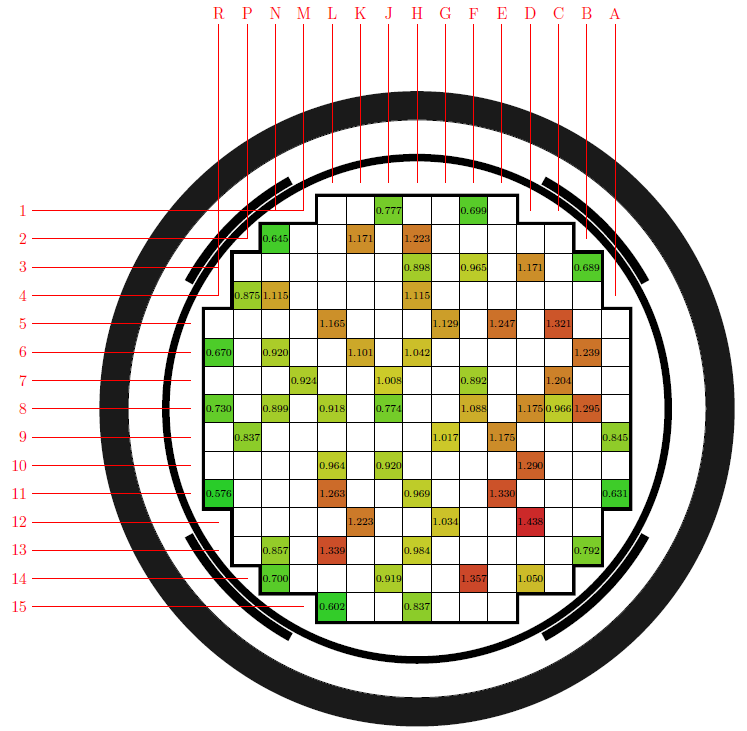
\includegraphics[keepaspectratio, width = 4.0 in]{figures/hzp_map}
\caption{Hot zero power radial detector measurements (axially integrated).}
\label{fig:fig_hzp_map}
\end{figure}


\subsection{Estimating uncertainty of axial detector data}

To evaluate uncertainties of the processed data, the uncertainties of the measured signals and those coming from post-processing are analyzed and combined.

The uncertainty of each axial detector data can be expressed as:

\begin{equation}
\begin{split}
\label{eq:measure_uncertainty}
  \left(\frac{\delta_\phi}{\phi} \right)_m & = \sqrt{\frac{\left(\frac{\partial \phi}{\partial D}\cdot \delta_d\right)^{2}+\left(\frac{\partial \phi}{\partial B}\cdot \delta_b\right)^{2}+\left(\frac{\partial \phi}{\partial G}\cdot \delta_g\right)^{2}+\left(\frac{\partial \phi}{\partial P}\cdot \delta_p\right)^{2}}{\phi^{2}}} \\
  &=\sqrt{\frac{{\delta_d}^{2}+{\delta_b}^{2}}{(D-B)^{2}}+\left(\frac{\delta_g}{G}\right)^{2}+\left(\frac{\delta_p}{P}\right)^{2}}
\end{split}
\end{equation}

\begin{equation}
\label{eq:combined_uncertainty}
  \left(\frac{\delta_\phi}{\phi} \right)_{ijk} = \sqrt{{\left(\frac{\delta_\phi}{\phi} \right)_m}^{2}+{\left(\frac{\delta_\phi}{\phi}\right)_{intp}}^{2}+{\left(\frac{\delta_\phi}{\phi}\right)_{align}}^{2}+{\left(\frac{\delta_\phi}{\phi}\right)_{spline}}^{2}}
\end{equation}
where $\delta_{d}$, $\delta_{b}$, $\delta_{q}$, $\delta_{p}$, the uncertainties of the detector signal, background, gain factor and core power respectively, contribute to the measurement uncertainty $\left(\frac{\delta_\phi}{\phi}\right)_m$, while $\left(\frac{\delta_\phi}{\phi}\right)_{intp}$,  $\left(\frac{\delta_\phi}{\phi}\right)_{align}$, and  $\left(\frac{\delta_\phi}{\phi}\right)_{spline}$,  are the uncertainties introduced by interpolation, realignment and spline fitting, respectively. 

\subsubsection{Uncertainty from measurement}
As shown in equation \ref{eq:measure_uncertainty}, the uncertainty of the axial flux has contributions from measuring the detector signal, the background, the gain and the core power. All types of measured data are gathered and statistical analysis is used to get the ranges and distributions of the measurements, as shown in figure \ref{fig:fig_ranges_measured_data} for cycle 1. It is found that:

\begin{figure}[ht]
\centering
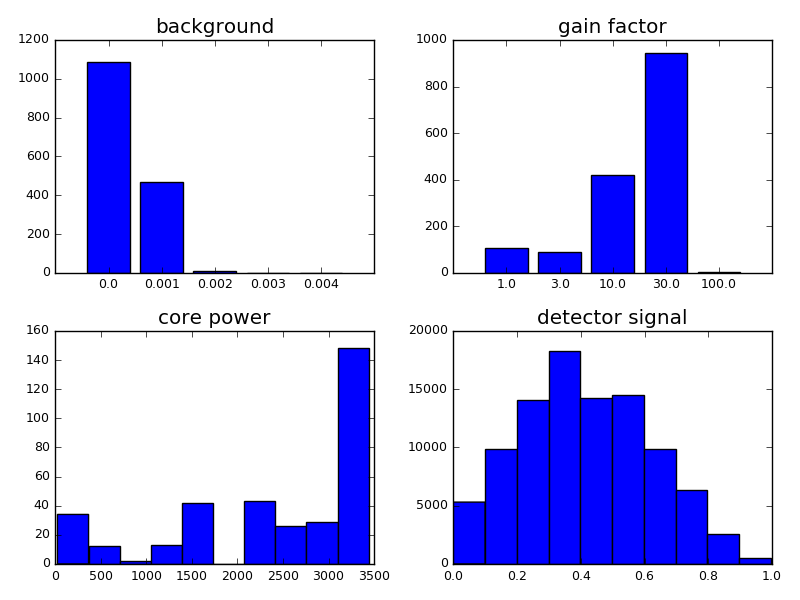
\includegraphics[keepaspectratio, width = 4.0 in]{figures/flux_map_uncertainties/ranges_measured_data}
\caption{Hot zero power radial detector measurements (axially integrated).}
\label{fig:fig_ranges_measured_data}
\end{figure}

\begin{enumerate}
\item The background values are very small, mostly provided by readings of 0 or 0.001. Accounting for the smallest division of the detector (0.001), uncertainty of the background can be estimated as half the smallest digit (0.0005) (i.e. $\delta_b=0.0005$). It should be noted that background is subtracted from detector signal and the detector signal is generally greater than 0.1 (0.41 on average), which implies from equation \ref{eq:measure_uncertainty} that both the effects of $B$ and $\delta_b$ are less than 0.1\% for most cases. 
\item The gain factors are discrete values which are selected before each pass. As there are actually only a few well-spaced out values, it is believed that the detector error caused by using different gain factors is negligible compared to other sources, i.e. $\delta_g$ is 0.
\item For almost all of the measurements the core is operated with powers in the 100 or 1000 of MWth.  As power is very important for normalization and values are reported with decimals, it can be safely assumed that its uncertainty ($\delta_p$) is less than 1.0\%, which also means that $\delta_p/P$ is under 0.1\%. 
\item Detector signal is the last remaining part. While the accuracy of detector is relative to specific measurements, literature indicates that for normal reactor applications that the uncertainty is on the order of 1\% \cite{mitelman2001core}. Therefore, it can be concluded qualitatively that the detector signal dominates the measurement uncertainty.
\end{enumerate}

Now the question becomes how to evaluate the uncertainty of measured data more accurately. Quantitatively, measurement uncertainty can be evaluated by performing repeated measurements and calculating the variance. Even though the reactor core monitoring is mostly carried out only once for each assembly, there are indeed certain locations that receive multiple measurements for redundancy. For example in cycle 1 of BEAVRS, there are about 180 cases each that have 2 or even 3 repeated measurements by the same detector in the same assembly. These multiple measurements are performed with the reactor core under almost the same conditions, such as control rod positions, boron concentration and coolant status. Core power as well as other measured parameters such as background, gain factor of detector may be slightly different but they will be accounted for in calculating axial flux. So the multiple measurements can be regarded as repeated data and their uncertainty represents the accuracy of the measured data. Figure \ref{fig:fig_multi_measure_H11}  is an example of multiple measurements which show the independent axial signals, mean and relative sample standard deviation (RSTD) of every axial measurement point.

\begin{figure}[ht]
\centering
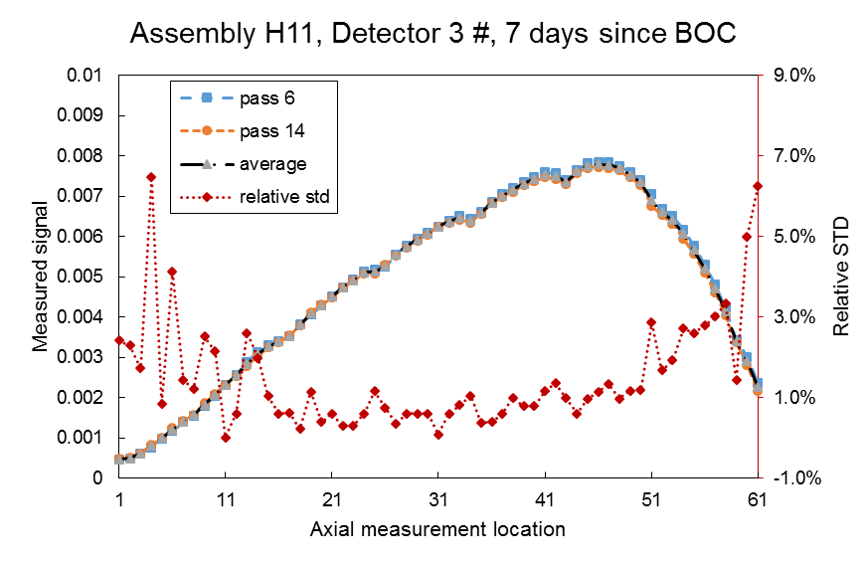
\includegraphics[keepaspectratio, width = 4.0 in]{figures/flux_map_uncertainties/Multi-Measurements-H11}
\caption{Multiple measurements example of H11 assembly}
\label{fig:fig_multi_measure_H11}
\end{figure}

Since there are mostly only 2 replicated measurements for each data point, the variance estimate is not likely to be accurate, thus gathering the data over multiple cases through the whole cycle is necessary to obtain a reliable uncertainty estimate.

Here we assume the measurement uncertainty is related only to the detector signal amplitude. That means the multiple measurement cases with similar mean value have similar uncertainty, therefore we can group the data points by amplitude and estimate an average uncertainty for each group. Specifically, the relative sample standard deviations are gathered and used to calculate the uncertainties of all groups. To make the estimate more conservative, a 95\% confidence value is adopted as resulting uncertainty. In calculation, all the data are sorted and the value at the 95\% position is selected. Note that the data points in one replicated measurement case follow the same Gaussian distribution. For each double repeated measurements case, it can be demonstrated that the relative sample standard deviation follows a distribution given by equation \ref{eq:rstd_dist} and the 95\% confidence value is actually equal to 2 times of true standard deviation i.e. $2\sigma$.

\begin{equation}
\label{eq:rstd_dist}
  f(s) = \frac{4}{\sqrt{2\pi\sigma}}e^{-\frac{s^2}{{\sigma}^2}}
\end{equation}

There are 11145 multiple measurements in cycle 1 and they are divided into 30 groups by signal amplitude with equal number of data points in each group. The 95\% confidence values are calculated for each group one by one, thus a table of signal ranges and measurement uncertainties is obtained, as shown in figure \ref{fig:fig_multi_measure_all} and \ref{fig:fig_measure_groups}.

\begin{figure}[ht]
\centering
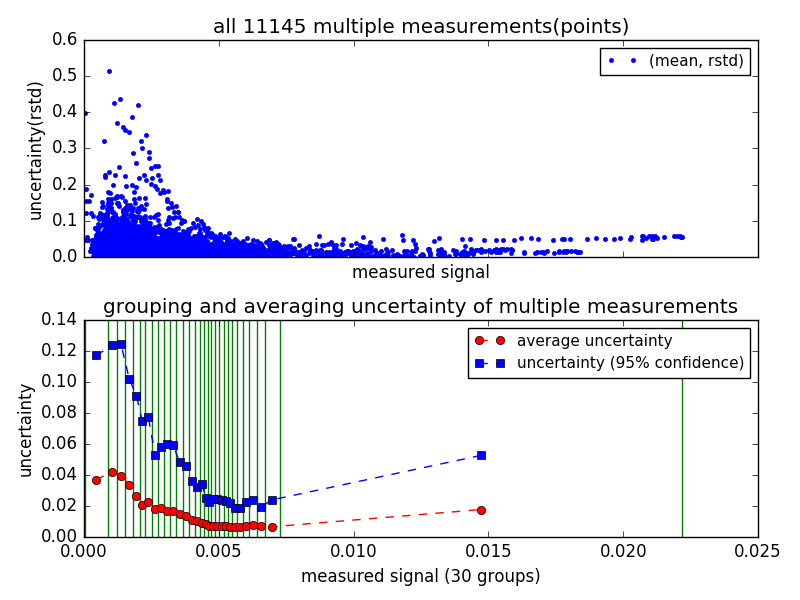
\includegraphics[keepaspectratio, width = 4.5 in]{figures/flux_map_uncertainties/multi_measure_all.png}
\caption{Axial signal uncertainty from all multiple measurements in cycle 1}
\label{fig:fig_multi_measure_all}
\end{figure}

\begin{figure}[ht]
\centering
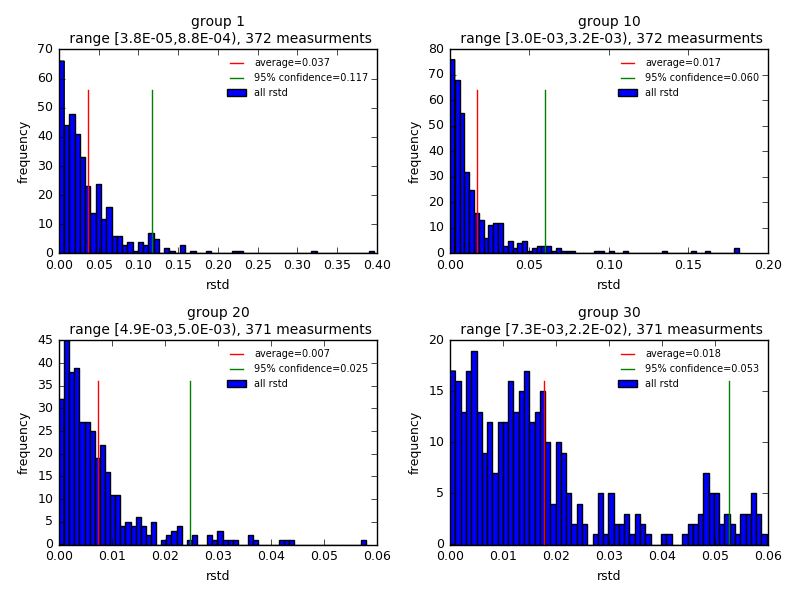
\includegraphics[keepaspectratio, width = 4.5 in]{figures/flux_map_uncertainties/multi_measure_groups.png}
\caption{Average and 95\% confidence values for each multiple measurements group}
\label{fig:fig_measure_groups}
\end{figure}

As can be found in figure \ref{fig:fig_multi_measure_all}, the axial measurement uncertainty is generally around 2 to 12\% and is dependent on signal amplitude, i.e. the greater the signal, the smaller the uncertainty. This look-up table can be applied to all detector signals to get the measurement uncertainties.


\subsubsection{Uncertainty from Processing}
To analyze the uncertainty caused by data post-processing such as interpolation, realignment and spline fitting, a method of observing the variation before and after the processing is used.

\paragraph{Interpolation}
\mbox{ }\\
The interpolation is performed when one data point is unrecorded. To estimate the error of interpolated data, we just eliminate one-by-one points that were properly recorded and then compare the axial relative error with the recorded data. Figure \ref{fig:fig_interp_error} displays all the interpolation errors and their averages along with axial locations.

Interpolation error is dependent of location and it is greater near endpoints or grids. Here again we use the 95\% confidence strategy for each location. The 95\% confidence values are collected as a look-up table to estimate the uncertainty of every interpolation performed during processing.

\begin{figure}[ht]
\centering
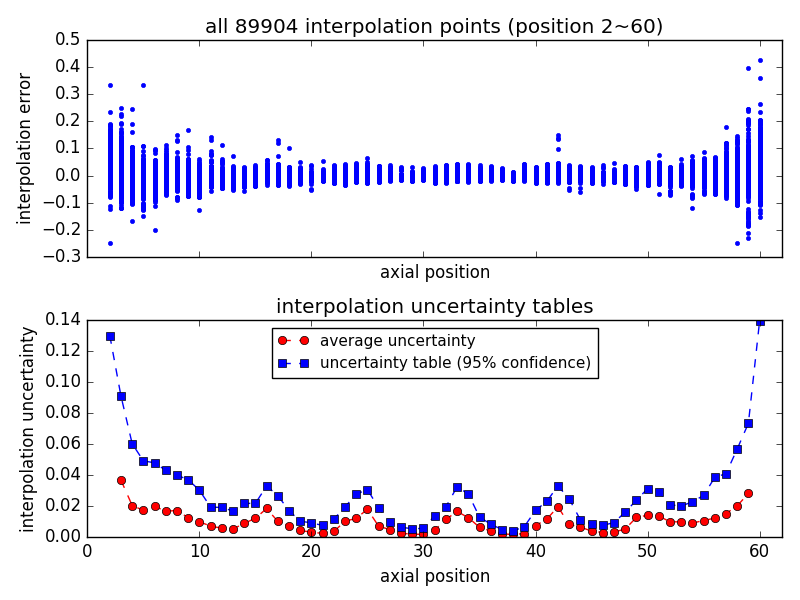
\includegraphics[keepaspectratio, width = 4.0 in]{figures/flux_map_uncertainties/interp_error.png}
\caption{Axial interpolation error}
\label{fig:fig_interp_error}
\end{figure}

\paragraph{Axial re-alignment}
\mbox{ }\\
Re-alignment of axial signals is carried out such that axial signals are provided over the active fuel length. But it should be noted that only the positions of the axial data are moved up or down in re-alignment. The data points themselves are kept unchanged and are believed accurate, except for the lost edge points which are calculated using extrapolation. Therefore, the error of re-alignment essentially comes from extrapolation of end points. A similar method to interpolation is used to estimate the error of these extrapolations, i.e. comparing normal measured data with extrapolated data. Axial measurements are re-aligned by 1 or 2 axial positions and in rare situations 3. Figure \ref{fig:fig_alignment_error_ex} shows an example of the effect of grid re-alignment.

\begin{figure}[ht]
\centering
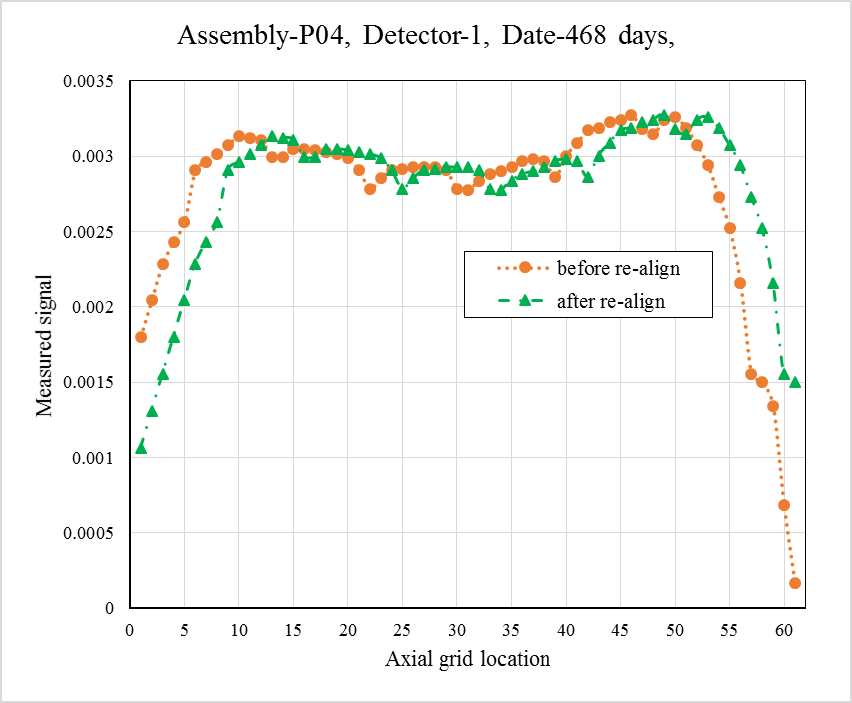
\includegraphics[keepaspectratio, width = 4.0 in]{figures/flux_map_uncertainties/Re-align_large_error.png}
\caption{Example of large re-alignment error}
\label{fig:fig_alignment_error_ex}
\end{figure}

Figure \ref{fig:fig_realgin_error} shows the error of axial re-alignment i.e. the relative error caused by extrapolation in 6 grid positions and the means of absolute errors. Again, these data will be used as a look-up table to estimate error of axial points which are extrapolated when re-alignment is performed.

\begin{figure}[ht]
\centering
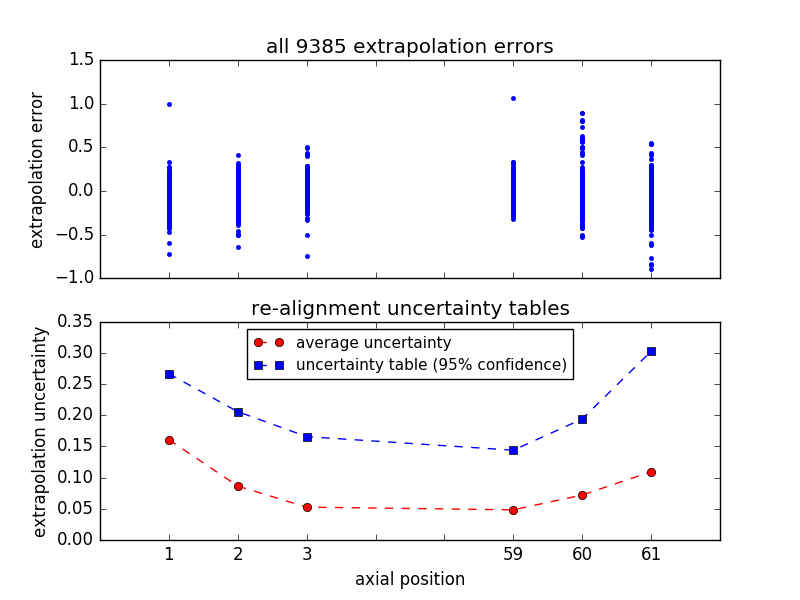
\includegraphics[keepaspectratio, width = 4.0 in]{figures/flux_map_uncertainties/realgin_error.png}
\caption{Axial re-alignment error}
\label{fig:fig_realgin_error}
\end{figure}

\paragraph{Spline fitting}
\mbox{ }\\
Spline fitting is used to put the detector signals on an axial coordinate grid corresponding to points that range from the bottom to the top of the active fuel. The error introduced in spline fitting is found negligible because the 2nd order spline fit is quite accurate and the errors are less than ${10}^{-10}$.

\begin{equation}
\label{eq:spline_error}
  \left(\frac{\delta_\phi}{\phi}\right)_{spline} \approx 0
\end{equation}

\subsubsection{Combining uncertainties}
Finally, the uncertainties of all axial signals can be quantified by calculating every independent uncertainty using the look-up tables and combining them together by the uncertainty equation i.e. in the following steps:

\begin{enumerate}
\item The measurement uncertainty $\left(\frac{\delta_\phi}{\phi}\right)_{m}$ is looked up according to the amplitude of calculated axial data.
\item If this data point is interpolated, an interpolation error $\left(\frac{\delta_\phi}{\phi}\right)_{intp}$ is looked up according to its location.
\item If this data point is realigned, an extrapolation error $\left(\frac{\delta_\phi}{\phi}\right)_{align}$ is looked up according to its location.
\item The square root of sum of squares of all uncertainties is calculated as resulting uncertainty $\left(\frac{\delta_\phi}{\phi}\right)_{ijk}$ for each data point.
\end{enumerate}

Figure \ref{fig:fig_combined_error} shows an example of combined axial signal uncertainty for one assembly in cycle 1.

\begin{figure}[ht]
\centering
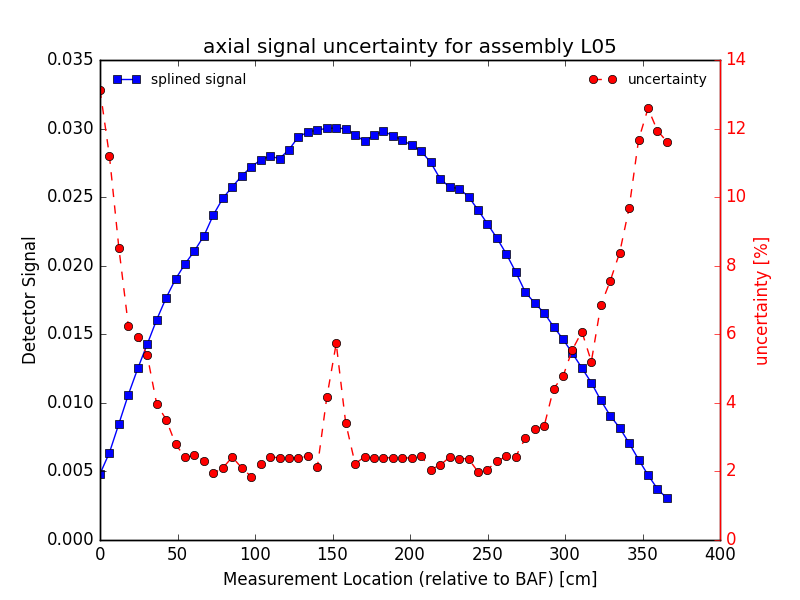
\includegraphics[keepaspectratio, width = 4.0 in]{figures/flux_map_uncertainties/combined_error.png}
\caption{Combined uncertainty of axial detector measurement - assembly L05 on day 54}
\label{fig:fig_combined_error}
\end{figure}

Since most of the measured data points are not affected by interpolation or realignment, the uncertainty of axial detector data is generally between 2 to 12\%.

\subsection{Uncertainty of axially integrated radial data}

Uncertainty of radial assembly data which is axially integrated can be evaluated by accounting for the errors of all axial points in one assembly, as indicated in equation \ref{eq:assem_uncertainty}.

\begin{equation}
\label{eq:assem_uncertainty}
  \left(\frac{\delta_\phi}{\phi} \right)_{ij} = \frac{\sqrt{\sum_{k=1}^K {\left(\delta_\phi\right)_{ijk}}^{2}}}{\phi_{ij}}
\end{equation}
where $i$, $j$ represent radial assembly position and $k$ for axial location.

For example, in assembly L05, the axial uncertainty shown in figure \ref{fig:fig_combined_error} can be substituted into the equation and an assembly uncertainty of 0.43\% is obtained.

Table \ref{table:radial_combined_all_day_66} gives full core radial detector measurements and calculated uncertainties on day 66 in cycle 1, while figure \ref{fig:fig_radial_combined_dist} gives the distribution of all assembly uncertainties in cycle 1. It can be seen the average uncertainty of radial measurements is around 0.6\% and 95\% confidence value is 1.2\%.

\begin{table}[ht]
  \centering
  \caption{Full core radial detector measurements and axially combined uncertainties on day 66}
  \label{table:radial_combined_all_day_66}
  \begin{tabular}{|r|l|c|r|l|}
    \hline
    K12 & 1.259 $\pm$ 0.39\% & & D10 & 1.271 $\pm$ 0.39\% \\ \hline 
    D12 & 1.209 $\pm$ 0.39\% & & H3 & 0.941 $\pm$ 0.55\% \\ \hline 
    H2 & 1.199 $\pm$ 0.41\% & & L10 & 1.047 $\pm$ 0.48\% \\ \hline 
    H6 & 1.254 $\pm$ 0.40\% & & L13 & 1.256 $\pm$ 0.40\% \\ \hline 
    F7 & 1.031 $\pm$ 0.49\% & & F1 & 0.643 $\pm$ 0.91\% \\ \hline 
    G9 & 1.234 $\pm$ 0.41\% & & F3 & 0.950 $\pm$ 0.55\% \\ \hline 
    F8 & 1.253 $\pm$ 0.40\% & & E11 & 1.328 $\pm$ 0.38\% \\ \hline 
    A11 & 0.544 $\pm$ 1.01\% & & R11 & 0.519 $\pm$ 1.06\% \\ \hline 
    E9 & 1.290 $\pm$ 0.38\% & & G12 & 1.046 $\pm$ 0.48\% \\ \hline 
    M7 & 1.018 $\pm$ 0.49\% & & N8 & 0.939 $\pm$ 0.55\% \\ \hline 
    L15 & 0.531 $\pm$ 1.02\% & & N6 & 0.936 $\pm$ 0.55\% \\ \hline 
    J10 & 1.048 $\pm$ 0.48\% & & N2 & 0.569 $\pm$ 0.95\% \\ \hline 
    K2 & 1.145 $\pm$ 0.42\% & & H13 & 0.973 $\pm$ 0.52\% \\ \hline 
    K6 & 1.294 $\pm$ 0.38\% & & L8 & 1.032 $\pm$ 0.50\% \\ \hline 
    H11 & 1.226 $\pm$ 1.06\% & & L5 & 1.284 $\pm$ 0.38\% \\ \hline 
    E5 & 1.305 $\pm$ 0.38\% & & H15 & 0.725 $\pm$ 0.81\% \\ \hline 
    D8 & 1.258 $\pm$ 0.40\% & & C8 & 0.954 $\pm$ 0.54\% \\ \hline 
    B3 & 0.576 $\pm$ 0.94\% & & B6 & 1.159 $\pm$ 0.42\% \\ \hline 
    B8 & 1.208 $\pm$ 0.41\% & & H4 & 1.248 $\pm$ 0.40\% \\ \hline 
    C5 & 1.250 $\pm$ 0.40\% & & F14 & 1.217 $\pm$ 0.41\% \\ \hline 
    C7 & 1.212 $\pm$ 0.41\% & & N13 & 0.708 $\pm$ 0.83\% \\ \hline 
    A9 & 0.738 $\pm$ 0.79\% & & N14 & 0.585 $\pm$ 0.93\% \\ \hline 
    R6 & 0.630 $\pm$ 0.92\% & & R8 & 0.690 $\pm$ 0.87\% \\ \hline 
    J8 & 0.936 $\pm$ 0.55\% & & P4 & 0.768 $\pm$ 0.78\% \\ \hline 
    J1 & 0.712 $\pm$ 0.83\% & & P9 & 0.798 $\pm$ 0.71\% \\ \hline 
    J7 & 1.219 $\pm$ 0.41\% & & B13 & 0.604 $\pm$ 0.92\% \\ \hline
  \end{tabular}
\end{table}

\begin{figure}[ht]
\centering
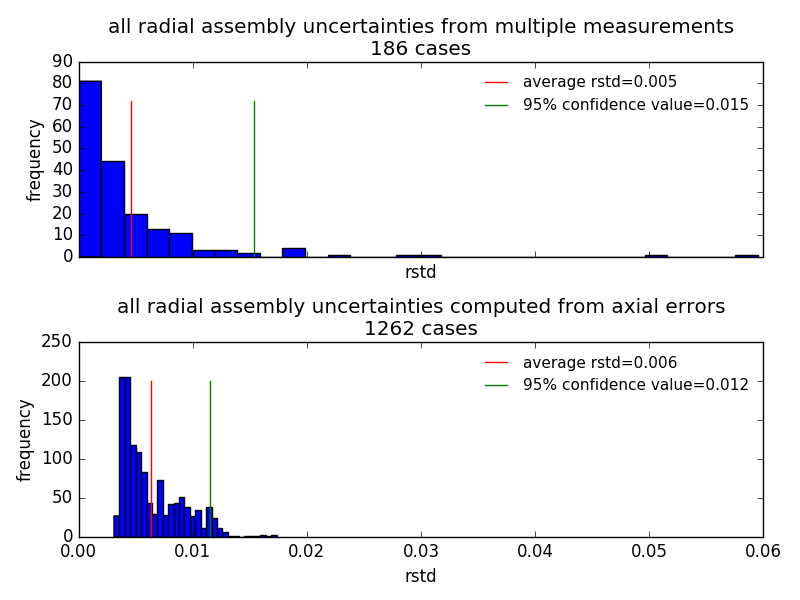
\includegraphics[keepaspectratio, width = 4.0 in]{figures/flux_map_uncertainties/radial_uncertainty_combined_dist.png}
\caption{Distribution of radial data uncertainty calculated from axial uncertainties in cycle 1}
\label{fig:fig_radial_combined_dist}
\end{figure}

The multiple measurements can also be used to quantify uncertainty of radial data as a second means. Similar to the treatment with the axial multiple signals, all multiple measurement cases of radial data are collected and statistics is made to estimate uncertainty of radial data, as shown in figure \ref{fig:fig_radial_multiple_dist}. There are 186 cases of multiple measurements in cycle 1. The average relative error is about 0.5\% while the 95\% confidence value is 1.5\%.

It should be noted the two ways to estimate radial uncertainty are somewhat independent with each other so verification can be performed between the two.  The two approaches are quite consistent with each other, as shown in figure \ref{fig:fig_radial_combined_dist} and figure \ref{fig:fig_radial_multiple_dist}. Therefore, it can be concluded the methodology to quantify the flux map uncertainties is basically correct and valid.

\begin{figure}[ht]
\centering
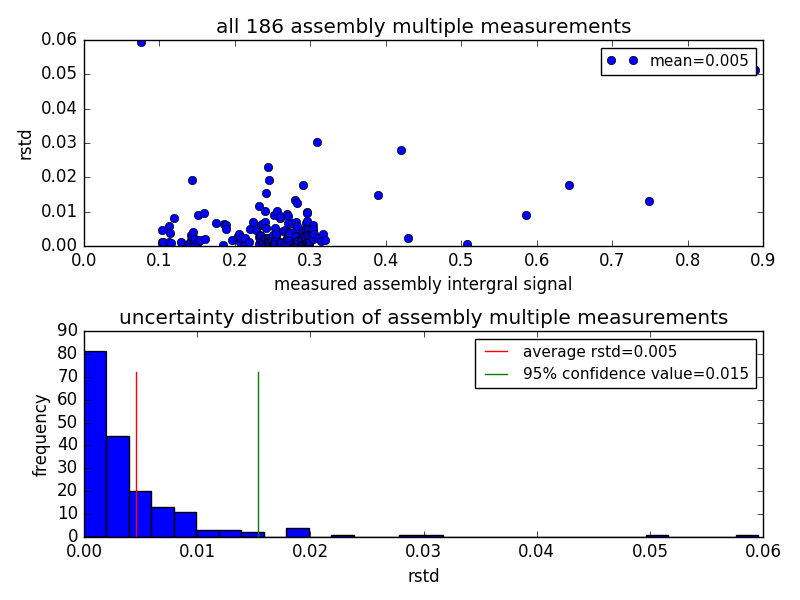
\includegraphics[keepaspectratio, width = 4.0 in]{figures/flux_map_uncertainties/radial_uncertainty_multiple_dist.png}
\caption{Distribution of radial data uncertainty using multiple measurements in cycle 1}
\label{fig:fig_radial_multiple_dist}
\end{figure}


\section{Task: HFP Boron Letdown Uncertainties}
The measured boron letdown curves during Cycle 1 and Cycle 2 operation are given in the BEAVRS benchmark, as shown in Figure \ref{fig:fig_boron_letdown}.

\begin{figure}[ht]
\centering
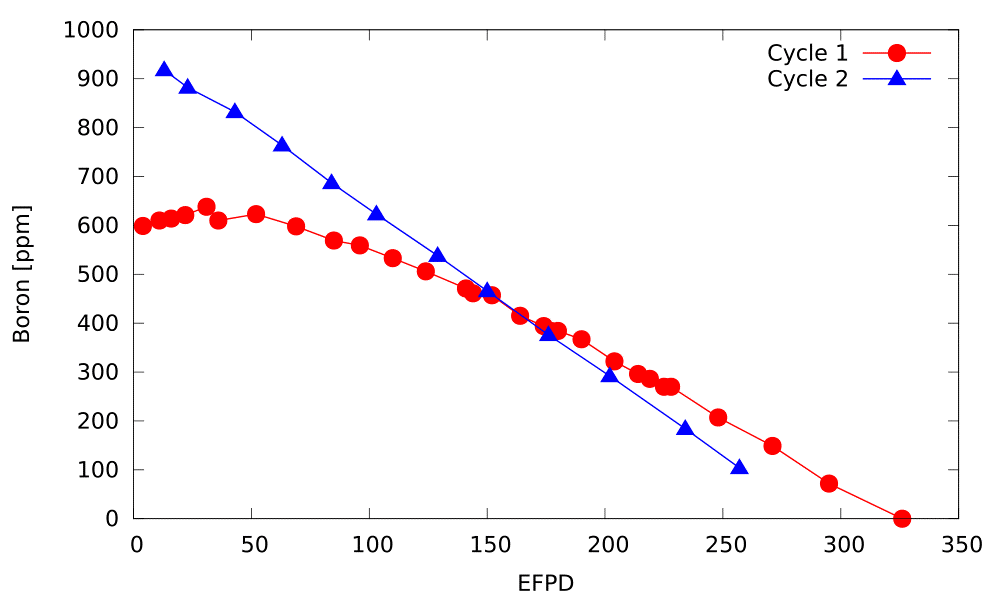
\includegraphics[keepaspectratio, width = 4.0 in]{figures/boron_letdown}
\caption{Boron letdown curves for two cycles of operation}
\label{fig:fig_boron_letdown}
\end{figure}

From literature review, the typical acceptance criteria from regulators is that codes must predict critical boron at +/- 50 ppm.  Recent measurements from low power physics tests of OPR reactors indicate measurement uncertainties below 1\% or about 10 ppm.

One way to evaluate boron measurement uncertainties is to estimate the accuracy of the boron meter (BM) used in the measurements. It is found in the original data files that multiple boron readings exists in some cases. Specifically, boron data is recorded for each detector pass thus the count of boron readings is equal to the number of detector passes, as shown in Table \ref{table:boron_multiple_data}. Since the measuring passes are carried out on the same day with control rods at the same positions, i.e. under almost the same core conditions, these multiple boron readings can be regarded as repeated independent measurements. Therefore, the standard deviation of the boron data should reveal to some extent the uncertainty of boron measurements.

\begin{table}[ht]
\centering
\caption{Repeated Boron measurements in cycle 1}
\label{table:boron_multiple_data}
\resizebox{\textwidth}{!}{%
\begin{tabular}{|l|l|l|}
\hline
days & \# of passes & Boron measurements (ppm)                                                                                                    \\ \hline
0    & 20           & \begin{tabular}[c]{@{}l@{}}973, 964, 964, 991, 969, 972, 962, 977, 984, 984, 981, 986, 956, 986,\\ 986, 991, 989, 973, 933, 984\end{tabular} \\ \hline
7    & 14           & 881, 880, 881, 875, 878, 873, 877, 877, 881, 877, 875, 873, 870, 877                                                        \\ \hline
18   & 14           & 792, 798, 795, 805, 809, 802, 800, 802, 798, 806, 800, 803, 809, 800                                                        \\ \hline
54   & 13           & 744, 761, 764, 753, 753, 752, 756, 769, 750, 745, 752, 762, 750                                                             \\ \hline
62   & 17           & \begin{tabular}[c]{@{}l@{}}705, 708, 698, 695, 703, 700, 700, 691, 711, 708, 705, 703, 706, 706,\\ 703, 709, 702\end{tabular} \\ \hline
66   & 25           & \begin{tabular}[c]{@{}l@{}}700, 708, 695, 702, 706, 700, 708, 697, 706, 692, 698, 697, 706, 703,\\ 694, 695, 697, 706, 697, 703, 695, 695, 697, 697, 706\end{tabular} \\ \hline
81   & 13           & 645, 645, 658, 648, 658, 647, 661, 645, 662, 644, 652, 658, 655                                                             \\ \hline
82   & 13           & 642, 648, 645, 645, 647, 648, 648, 647, 645, 647, 647, 641, 616                                                             \\ \hline
88   & 13           & 630, 631, 639, 634, 630, 634, 634, 630, 631, 630, 631, 631, 636                                                             \\ \hline
92   & 13           & 608, 606, 627, 631, 634, 633, 631, 622, 634, 617, 623, 616, 612                                                             \\ \hline
161  & 16           & \begin{tabular}[c]{@{}l@{}}695, 692, 703, 702, 698, 700, 705, 700, 702, 702, 702, 700, 691, 689,\\ 700, 695\end{tabular} \\ \hline
169  & 14           & 631, 630, 628, 633, 630, 627, 630, 630, 628, 628, 630, 633, 630, 630                                                        \\ \hline
187  & 14           & 622, 620, 619, 619, 617, 641, 620, 620, 619, 619, 622, 622, 620, 614                                                        \\ \hline
218  & 13           & 575, 577, 578, 580, 577, 580, 580, 578, 578, 575, 581, 580, 578                                                             \\ \hline
251  & 13           & 520, 514, 520, 516, 523, 516, 514, 514, 516, 519, 514, 520, 514                                                             \\ \hline
323  & 11           & 531, 530, 525, 527, 522, 523, 530, 523, 527, 528, 522                                                                       \\ \hline
339  & 12           & 437, 436, 436, 433, 439, 436, 442, 434, 441, 436, 439, 434                                                                  \\ \hline
368  & 14           & 439, 430, 423, 377, 362, 359, 369, 366, 364, 373, 373, 375, 380, 375                                                        \\ \hline
403  & 11           & 306, 305, 305, 305, 309, 305, 308, 305, 308, 305, 306                                                                       \\ \hline
\end{tabular}}
\end{table}

The accuracy of boron instrument can be calculated from the statistical properties of the repeated measurements, as shown in the following equations.

\begin{equation}
\label{eq:boron_uncertainty_1}
  X=\frac{1}{N}\sum_{i=1}^N {x_i}
\end{equation}
\begin{equation}
\label{eq:boron_uncertainty_2}
  \Delta{X}=\frac{1}{N}\sqrt{\sum_{i=1}^N {\Delta{{x_i}}^{2}}}=\frac{1}{\sqrt{N}}\Delta{x}
\end{equation}
\begin{equation}
\label{eq:boron_uncertainty_3}
  \Delta{x}=\sqrt{N} \Delta{X} \approx \sqrt{N} \cdot {STD}
\end{equation}
where $x$ is the boron measurement, $X$ is the average of multiple measurements, $N$ is the number of independent measurements, $\Delta{x}$ is the accuracy of boron meter(BM) and $\Delta{X}$ is the uncertainty of multiple measurements which can be represented by the standard deviation (${STD}$).

Table \ref{table:boron_uncertainty_multiple} gives estimations of BM accuracies for all the 19 multiple measurements cases. The average of all instances is 24.3 ppm. It should be noted that even though the boron meter accuracy is fluctuating due to the insufficient repeated measurements for every single case, the average of all these instances provides a reasonable estimate because the number of total cases (273) is quite large. Thus, the preliminary estimation of boron measurement uncertainty is around 25 ppm from the current approach.

\begin{table}[ht]
\centering
\caption{Calculating boron meter accuracy from multiple measurements}
\label{table:boron_uncertainty_multiple}
\begin{tabular}{|c|c|c|c|}
\hline
days & N  & Standard deviation (ppm) & BM accuracy (ppm) \\ \hline
0    & 20 & 14.4                     & 64.4              \\ \hline
7    & 14 & 3.4                      & 12.6              \\ \hline
18   & 14 & 4.9                      & 18.3              \\ \hline
54   & 13 & 7.4                      & 26.7              \\ \hline
62   & 17 & 5.2                      & 21.3              \\ \hline
66   & 25 & 4.9                      & 24.7              \\ \hline
81   & 13 & 6.8                      & 24.4              \\ \hline
82   & 13 & 8.6                      & 30.9              \\ \hline
88   & 13 & 2.8                      & 10.1              \\ \hline
92   & 13 & 10.0                     & 36.1              \\ \hline
161  & 16 & 4.7                      & 18.9              \\ \hline
169  & 14 & 1.7                      & 6.5               \\ \hline
187  & 14 & 6.1                      & 22.9              \\ \hline
218  & 13 & 1.9                      & 6.9               \\ \hline
251  & 13 & 3.1                      & 11.2              \\ \hline
323  & 11 & 3.4                      & 11.2              \\ \hline
339  & 12 & 2.8                      & 9.7               \\ \hline
368  & 14 & 26.6                     & 99.4              \\ \hline
403  & 11 & 1.5                      & 5.0               \\ \hline
\multicolumn{3}{|c|}{average}        & 24.3              \\ \hline
\end{tabular}
\end{table}

An alternative way to quantifying the boron letdown uncertainty is to compare measurements with the code calculation. Here, CASMO-5/Simulate-3 codes are used to model the BEAVRS benchmark and boron letdown values are calculated along with the benchmark burnup points. Table \ref{table:table:boron_uncertainty_simulation} presents the measured and calculated values and their discrepancies in Cycle 1. It can be seen that the average discrepancy is 25.2 ppm, which has good agreement with the above boron measurement uncertainty estimated from multiple measurements. Therefore, the boron uncertainty of 25 ppm seems appropriate.

\begin{table}[ht]
\centering
\caption{Comparison of measured boron level with CASMO/Simulate calculated boron in Cycle 1}
\label{table:table:boron_uncertainty_simulation}
\begin{tabular}{|c|c|c|c|}
\hline
\begin{tabular}[c]{@{}c@{}}Burnup\\ (MWd/kg)\end{tabular} & \begin{tabular}[c]{@{}c@{}}Measured Boron\\ (ppm)\end{tabular} & \begin{tabular}[c]{@{}c@{}}Calculated Boron\\ (ppm)\end{tabular} & \begin{tabular}[c]{@{}c@{}}Absolute error\\ (ppm)\end{tabular} \\ \hline
0               & 975.25               & 958                    & 17.3                 \\ \hline
0.04            & 801.36               & 784                    & 17.4                 \\ \hline
0.15            & 754.69               & 712                    & 42.7                 \\ \hline
0.27            & 703.12               & 670                    & 33.1                 \\ \hline
0.33            & 700                  & 666                    & 34.0                 \\ \hline
0.64            & 652.15               & 626                    & 26.2                 \\ \hline
0.67            & 643.54               & 626                    & 17.5                 \\ \hline
0.88            & 632.38               & 611                    & 21.4                 \\ \hline
1.02            & 622.62               & 598                    & 24.6                 \\ \hline
1.3             & 698.5                & 650                    & 48.5                 \\ \hline
1.51            & 629.86               & 602                    & 27.9                 \\ \hline
2.16            & 621                  & 588                    & 33.0                 \\ \hline
3.3             & 578.23               & 562                    & 16.2                 \\ \hline
4.61            & 516.92               & 503                    & 13.9                 \\ \hline
6.01            & 526.18               & 493                    & 33.2                 \\ \hline
6.49            & 436.92               & 418                    & 18.9                 \\ \hline
7.51            & 383.21               & 365                    & 18.2                 \\ \hline
8.7             & 306.09               & 298                    & 8.1                  \\ \hline
9.8             & 259                  & 231                    & 28.0                 \\ \hline
11.08           & 180                  & 153                    & 27.0                 \\ \hline
12.34           & 120                  & 74                     & 46.0                 \\ \hline
12.92           & 50                   & 64                     & 14.0                 \\ \hline
13.6            & 35                   & 48                     & 13.0                 \\ \hline
\multicolumn{3}{|c|}{average}                                   & 25.2                 \\ \hline
\end{tabular}
\end{table}

\FloatBarrier
\clearpage


\section{Task: Time Series Analysis}

The BEAVRS Year 2 Report \cite{liang_year2_report} develops the framework for quantifying time-dependent uncertainty using the linear model as well as the CASMO/Simulate model, and the Year 3 Report \cite{kumar_year3_report} expands on this work to attribute overall uncertainty values to such models. This uncertainty is composed of error that arises from assuming a linear tilt-correction to BEAVRS data, which is discussed in Section \ref{sec:tiltcorr-unc}. In addition, Sections \ref{sec:cassim-unc} and \ref{sec:lm_uq} look at the second source of time-dependent uncertainty - detection uncertainty - which is induced from fitting a simulation model to assembly-level BEAVRS data. In the case of Section \ref{sec:cassim-unc}, the simulation model under consideration is the CASMO/Simulate model, while Section \ref{sec:lm_uq} examines the validity of using the linear regression model instead. Finally, Section \ref{sec:timeseries_summary} summaries the findings from this task.

\subsection{Uncertainty in Using Tilt-Corrected BEAVRS Data}\label{sec:tiltcorr-unc}

The BEAVRS Year 1 Report \cite{liang_year1_report} introduces the need for a tilt corrected BEAVRS data set. The rationale for this can be understood by looking at Figure \ref{fig:fig_hzp_map}, which plots the original BEAVRS measured data at HZP. It can be seen that the reaction rate data is not eighth-core symmetric despite a symmetric core loading pattern, with the exception of instrumentation tubes and as-built masses. This tilt was first described in detail by Sykora in his Master's thesis, where he devises an algorithm to remove this tilt to yield eighth-core symmetric reaction rates \cite{sykora_ms}. The magnitude of this tilt is not fixed, however, and slowly decreases over burnup. Eliminating the tilt is essential in the process of fitting the CASMO/Simulate model to BEAVRS data, which is explored in Section \ref{sec:cassim-unc}. This is because simulation tools will produce symmetric results given a symmetric core loading pattern and cannot arbitrarily impose a tilt to mimic that observed in the BEAVRS data. Thus, tilt correction allows for a more accurate comparison between operational and simulated data, but artificially masks an un-modeled phenomenon within the operating data. The exact amount of added uncertainty from assuming a linear tilt correction is the focus of this section. A linear tilt performed best in terms of modeling the tilt observed within operating data. Section \ref{sec:gen_tc_data} explores the process of identifying the best x-y plane to fit BEAVRS data, while Section \ref{sec:tc_uq_method} devises a comprehensive method for simulating the tilt observed in the BEAVRS data. Finally, Section \ref{sec:tc_uq_eval} uses the radial map that results from this revised approach as a basis for evaluating tilt-correction uncertainty.

\definecolor{Dfourteencolor}{rgb}{0.789814983705,0.8,0.16}
\definecolor{Ntwocolor}{rgb}{0.359778907148,0.8,0.16}
\definecolor{Gsevencolor}{rgb}{0.8,0.719677085841,0.16}
\definecolor{Gsixcolor}{rgb}{0.688040431713,0.8,0.16}
\definecolor{Gfivecolor}{rgb}{0.8,0.497077458007,0.16}
\definecolor{Gfourcolor}{rgb}{0.8,0.781932225152,0.16}
\definecolor{Gthreecolor}{rgb}{0.8,0.455338457712,0.16}
\definecolor{Gtwocolor}{rgb}{0.64660573992,0.8,0.16}
\definecolor{Gonecolor}{rgb}{0.548821323754,0.8,0.16}
\definecolor{Nfourcolor}{rgb}{0.8,0.409103287753,0.16}
\definecolor{Kfourteencolor}{rgb}{0.8,0.330954155744,0.16}
\definecolor{Gninecolor}{rgb}{0.8,0.719677085841,0.16}
\definecolor{Geightcolor}{rgb}{0.488772261109,0.8,0.16}
\definecolor{Nsixcolor}{rgb}{0.8,0.765985546612,0.16}
\definecolor{Nsevencolor}{rgb}{0.8,0.455338457712,0.16}
\definecolor{Rfivecolor}{rgb}{0.16,0.8,0.16}
\definecolor{Rsixcolor}{rgb}{0.402585601218,0.8,0.16}
\definecolor{Rsevencolor}{rgb}{0.548821323754,0.8,0.16}
\definecolor{Reightcolor}{rgb}{0.487422829174,0.8,0.16}
\definecolor{Rninecolor}{rgb}{0.548821323754,0.8,0.16}
\definecolor{Jeightcolor}{rgb}{0.488772261109,0.8,0.16}
\definecolor{Jninecolor}{rgb}{0.8,0.719677085841,0.16}
\definecolor{Jfourcolor}{rgb}{0.8,0.781932225152,0.16}
\definecolor{Jfivecolor}{rgb}{0.8,0.497077458007,0.16}
\definecolor{Jsixcolor}{rgb}{0.688040431713,0.8,0.16}
\definecolor{Jsevencolor}{rgb}{0.8,0.719677085841,0.16}
\definecolor{Jonecolor}{rgb}{0.548821323754,0.8,0.16}
\definecolor{Jtwocolor}{rgb}{0.64660573992,0.8,0.16}
\definecolor{Jthreecolor}{rgb}{0.8,0.455338457712,0.16}
\definecolor{Bfourcolor}{rgb}{0.789814983705,0.8,0.16}
\definecolor{Bfivecolor}{rgb}{1,1,1}
\definecolor{Bsixcolor}{rgb}{0.8,0.330954155744,0.16}
\definecolor{Bsevencolor}{rgb}{0.64660573992,0.8,0.16}
\definecolor{Bthreecolor}{rgb}{0.359778907148,0.8,0.16}
\definecolor{Ksevencolor}{rgb}{0.688040431713,0.8,0.16}
\definecolor{Beightcolor}{rgb}{0.8,0.293519413221,0.16}
\definecolor{Bninecolor}{rgb}{0.64660573992,0.8,0.16}
\definecolor{Ksixcolor}{rgb}{0.8,0.50670156813,0.16}
\definecolor{Nfivecolor}{rgb}{0.8,0.221326077279,0.16}
\definecolor{Kfivecolor}{rgb}{0.8,0.792925630235,0.16}
\definecolor{Lfourteencolor}{rgb}{1,1,1}
\definecolor{Lfifteencolor}{rgb}{0.16,0.8,0.16}
\definecolor{Kfourcolor}{rgb}{0.8,0.381640053048,0.16}
\definecolor{Ltencolor}{rgb}{0.8,0.792925630235,0.16}
\definecolor{Lelevencolor}{rgb}{0.8,0.319122460115,0.16}
\definecolor{Ltwelvecolor}{rgb}{1,1,1}
\definecolor{Lthirteencolor}{rgb}{0.8,0.221326077279,0.16}
\definecolor{Mfivecolor}{rgb}{1,1,1}
\definecolor{Mfourcolor}{rgb}{0.8,0.16,0.16}
\definecolor{Msevencolor}{rgb}{0.8,0.781932225152,0.16}
\definecolor{Msixcolor}{rgb}{0.8,0.381640053048,0.16}
\definecolor{Mthreecolor}{rgb}{0.8,0.409103287753,0.16}
\definecolor{Mtwocolor}{rgb}{0.789814983705,0.8,0.16}
\definecolor{Mninecolor}{rgb}{0.8,0.781932225152,0.16}
\definecolor{Meightcolor}{rgb}{0.8,0.491512764085,0.16}
\definecolor{Rtencolor}{rgb}{0.402585601218,0.8,0.16}
\definecolor{Relevencolor}{rgb}{0.16,0.8,0.16}
\definecolor{Mfourteencolor}{rgb}{0.789814983705,0.8,0.16}
\definecolor{Ptencolor}{rgb}{0.8,0.330954155744,0.16}
\definecolor{Pelevencolor}{rgb}{1,1,1}
\definecolor{Ptwelvecolor}{rgb}{0.789814983705,0.8,0.16}
\definecolor{Pthirteencolor}{rgb}{0.359778907148,0.8,0.16}
\definecolor{Eninecolor}{rgb}{0.8,0.497077458007,0.16}
\definecolor{Eeightcolor}{rgb}{0.759638588669,0.8,0.16}
\definecolor{Efivecolor}{rgb}{0.8,0.319122460115,0.16}
\definecolor{Efourcolor}{rgb}{1,1,1}
\definecolor{Esevencolor}{rgb}{0.8,0.497077458007,0.16}
\definecolor{Esixcolor}{rgb}{0.8,0.792925630235,0.16}
\definecolor{Eonecolor}{rgb}{0.16,0.8,0.16}
\definecolor{Peightcolor}{rgb}{0.8,0.293519413221,0.16}
\definecolor{Ethreecolor}{rgb}{0.8,0.221326077279,0.16}
\definecolor{Etwocolor}{rgb}{1,1,1}
\definecolor{Pthreecolor}{rgb}{0.359778907148,0.8,0.16}
\definecolor{Pninecolor}{rgb}{0.64660573992,0.8,0.16}
\definecolor{Psixcolor}{rgb}{0.8,0.330954155744,0.16}
\definecolor{Psevencolor}{rgb}{0.64660573992,0.8,0.16}
\definecolor{Pfourcolor}{rgb}{0.789814983705,0.8,0.16}
\definecolor{Pfivecolor}{rgb}{1,1,1}
\definecolor{Htencolor}{rgb}{0.8,0.628792138108,0.16}
\definecolor{Helevencolor}{rgb}{0.759638588669,0.8,0.16}
\definecolor{Htwelvecolor}{rgb}{0.8,0.491512764085,0.16}
\definecolor{Hthirteencolor}{rgb}{0.752384873822,0.8,0.16}
\definecolor{Hfourteencolor}{rgb}{0.8,0.293519413221,0.16}
\definecolor{Hfifteencolor}{rgb}{0.487422829174,0.8,0.16}
\definecolor{Ftwelvecolor}{rgb}{0.8,0.381640053048,0.16}
\definecolor{Fthirteencolor}{rgb}{0.8,0.765985546612,0.16}
\definecolor{Ftencolor}{rgb}{0.8,0.50670156813,0.16}
\definecolor{Felevencolor}{rgb}{0.8,0.792925630235,0.16}
\definecolor{Ffourteencolor}{rgb}{0.8,0.330954155744,0.16}
\definecolor{Ffifteencolor}{rgb}{0.402585601218,0.8,0.16}
\definecolor{Ntwelvecolor}{rgb}{0.8,0.409103287753,0.16}
\definecolor{Nthirteencolor}{rgb}{0.611249088254,0.8,0.16}
\definecolor{Heightcolor}{rgb}{1,1,1}
\definecolor{Nelevencolor}{rgb}{0.8,0.221326077279,0.16}
\definecolor{Nfourteencolor}{rgb}{0.359778907148,0.8,0.16}
\definecolor{Htwocolor}{rgb}{0.8,0.293519413221,0.16}
\definecolor{Hthreecolor}{rgb}{0.752384873822,0.8,0.16}
\definecolor{Honecolor}{rgb}{0.487422829174,0.8,0.16}
\definecolor{Hsixcolor}{rgb}{0.8,0.628792138108,0.16}
\definecolor{Hsevencolor}{rgb}{0.488772261109,0.8,0.16}
\definecolor{Hfourcolor}{rgb}{0.8,0.491512764085,0.16}
\definecolor{Hfivecolor}{rgb}{0.759638588669,0.8,0.16}
\definecolor{Kthirteencolor}{rgb}{0.8,0.765985546612,0.16}
\definecolor{Ktwelvecolor}{rgb}{0.8,0.381640053048,0.16}
\definecolor{Kelevencolor}{rgb}{0.8,0.792925630235,0.16}
\definecolor{Ktencolor}{rgb}{0.8,0.50670156813,0.16}
\definecolor{Dtencolor}{rgb}{0.8,0.381640053048,0.16}
\definecolor{Delevencolor}{rgb}{1,1,1}
\definecolor{Dtwelvecolor}{rgb}{0.8,0.16,0.16}
\definecolor{Dthirteencolor}{rgb}{0.8,0.409103287753,0.16}
\definecolor{Kthreecolor}{rgb}{0.8,0.765985546612,0.16}
\definecolor{Ktwocolor}{rgb}{0.8,0.330954155744,0.16}
\definecolor{Konecolor}{rgb}{0.402585601218,0.8,0.16}
\definecolor{Btwelvecolor}{rgb}{0.789814983705,0.8,0.16}
\definecolor{Bthirteencolor}{rgb}{0.359778907148,0.8,0.16}
\definecolor{Btencolor}{rgb}{0.8,0.330954155744,0.16}
\definecolor{Belevencolor}{rgb}{1,1,1}
\definecolor{Kninecolor}{rgb}{0.688040431713,0.8,0.16}
\definecolor{Keightcolor}{rgb}{0.8,0.628792138108,0.16}
\definecolor{Nthreecolor}{rgb}{0.611249088254,0.8,0.16}
\definecolor{Cninecolor}{rgb}{0.8,0.455338457712,0.16}
\definecolor{Ceightcolor}{rgb}{0.752384873822,0.8,0.16}
\definecolor{Cthreecolor}{rgb}{0.611249088254,0.8,0.16}
\definecolor{Ctwocolor}{rgb}{0.359778907148,0.8,0.16}
\definecolor{Kfifteencolor}{rgb}{0.402585601218,0.8,0.16}
\definecolor{Jfifteencolor}{rgb}{0.548821323754,0.8,0.16}
\definecolor{Csevencolor}{rgb}{0.8,0.455338457712,0.16}
\definecolor{Csixcolor}{rgb}{0.8,0.765985546612,0.16}
\definecolor{Cfivecolor}{rgb}{0.8,0.221326077279,0.16}
\definecolor{Cfourcolor}{rgb}{0.8,0.409103287753,0.16}
\definecolor{Etwelvecolor}{rgb}{1,1,1}
\definecolor{Ntencolor}{rgb}{0.8,0.765985546612,0.16}
\definecolor{Neightcolor}{rgb}{0.752384873822,0.8,0.16}
\definecolor{Nninecolor}{rgb}{0.8,0.455338457712,0.16}
\definecolor{Hninecolor}{rgb}{0.488772261109,0.8,0.16}
\definecolor{Gfifteencolor}{rgb}{0.548821323754,0.8,0.16}
\definecolor{Gfourteencolor}{rgb}{0.64660573992,0.8,0.16}
\definecolor{Gthirteencolor}{rgb}{0.8,0.455338457712,0.16}
\definecolor{Gtwelvecolor}{rgb}{0.8,0.781932225152,0.16}
\definecolor{Gelevencolor}{rgb}{0.8,0.497077458007,0.16}
\definecolor{Gtencolor}{rgb}{0.688040431713,0.8,0.16}
\definecolor{Fonecolor}{rgb}{0.402585601218,0.8,0.16}
\definecolor{Ftwocolor}{rgb}{0.8,0.330954155744,0.16}
\definecolor{Fthreecolor}{rgb}{0.8,0.765985546612,0.16}
\definecolor{Ffourcolor}{rgb}{0.8,0.381640053048,0.16}
\definecolor{Ffivecolor}{rgb}{0.8,0.792925630235,0.16}
\definecolor{Fsixcolor}{rgb}{0.8,0.50670156813,0.16}
\definecolor{Fsevencolor}{rgb}{0.688040431713,0.8,0.16}
\definecolor{Feightcolor}{rgb}{0.8,0.628792138108,0.16}
\definecolor{Fninecolor}{rgb}{0.688040431713,0.8,0.16}
\definecolor{Jthirteencolor}{rgb}{0.8,0.455338457712,0.16}
\definecolor{Melevencolor}{rgb}{1,1,1}
\definecolor{Mtencolor}{rgb}{0.8,0.381640053048,0.16}
\definecolor{Mthirteencolor}{rgb}{0.8,0.409103287753,0.16}
\definecolor{Mtwelvecolor}{rgb}{0.8,0.16,0.16}
\definecolor{Jtencolor}{rgb}{0.688040431713,0.8,0.16}
\definecolor{Jelevencolor}{rgb}{0.8,0.497077458007,0.16}
\definecolor{Eelevencolor}{rgb}{0.8,0.319122460115,0.16}
\definecolor{Etencolor}{rgb}{0.8,0.792925630235,0.16}
\definecolor{Ethirteencolor}{rgb}{0.8,0.221326077279,0.16}
\definecolor{Jfourteencolor}{rgb}{0.64660573992,0.8,0.16}
\definecolor{Efifteencolor}{rgb}{0.16,0.8,0.16}
\definecolor{Efourteencolor}{rgb}{1,1,1}
\definecolor{Cthirteencolor}{rgb}{0.611249088254,0.8,0.16}
\definecolor{Ctwelvecolor}{rgb}{0.8,0.409103287753,0.16}
\definecolor{Celevencolor}{rgb}{0.8,0.221326077279,0.16}
\definecolor{Ctencolor}{rgb}{0.8,0.765985546612,0.16}
\definecolor{Cfourteencolor}{rgb}{0.359778907148,0.8,0.16}
\definecolor{Aelevencolor}{rgb}{0.16,0.8,0.16}
\definecolor{Atencolor}{rgb}{0.402585601218,0.8,0.16}
\definecolor{Afivecolor}{rgb}{0.16,0.8,0.16}
\definecolor{Asevencolor}{rgb}{0.548821323754,0.8,0.16}
\definecolor{Asixcolor}{rgb}{0.402585601218,0.8,0.16}
\definecolor{Aninecolor}{rgb}{0.548821323754,0.8,0.16}
\definecolor{Aeightcolor}{rgb}{0.487422829174,0.8,0.16}
\definecolor{Jtwelvecolor}{rgb}{0.8,0.781932225152,0.16}
\definecolor{Lsixcolor}{rgb}{0.8,0.792925630235,0.16}
\definecolor{Lsevencolor}{rgb}{0.8,0.497077458007,0.16}
\definecolor{Lfourcolor}{rgb}{1,1,1}
\definecolor{Lfivecolor}{rgb}{0.8,0.319122460115,0.16}
\definecolor{Ltwocolor}{rgb}{1,1,1}
\definecolor{Lthreecolor}{rgb}{0.8,0.221326077279,0.16}
\definecolor{Lonecolor}{rgb}{0.16,0.8,0.16}
\definecolor{Leightcolor}{rgb}{0.759638588669,0.8,0.16}
\definecolor{Lninecolor}{rgb}{0.8,0.497077458007,0.16}
\definecolor{Deightcolor}{rgb}{0.8,0.491512764085,0.16}
\definecolor{Dninecolor}{rgb}{0.8,0.781932225152,0.16}
\definecolor{Dsixcolor}{rgb}{0.8,0.381640053048,0.16}
\definecolor{Dsevencolor}{rgb}{0.8,0.781932225152,0.16}
\definecolor{Dfourcolor}{rgb}{0.8,0.16,0.16}
\definecolor{Dfivecolor}{rgb}{1,1,1}
\definecolor{Dtwocolor}{rgb}{0.789814983705,0.8,0.16}
\definecolor{Dthreecolor}{rgb}{0.8,0.409103287753,0.16}

\begin{figure}[!htb]
    \centering
    
    % these dimensions are determined in arrow_dimms.ods

    \def\scale{1.6}

    \def\latWidth{0.2673473684*\scale}
    
    \def\RPVOR{3*\scale}
    \def\rectW{0.75*\scale}
    \def\RPVIR{2.7315789474*\scale}
    \def\BarrelIR{2.3368421053*\scale}
    \def\BarrelOR{2.4078947368*\scale}
    \def\ShieldIR{2.4223787816*\scale}
    \def\ShieldOR{2.5067965189*\scale}
    \def\LinerIR{2.7246166598*\scale}

    \def\bafCIRx{0.9357157895*\scale}
    \def\bafCIRy{2.0051052632*\scale}
    \def\bafCORx{0.9633473684*\scale}
    \def\bafCORy{2.0327368421*\scale}
    \def\bafMIRx{1.7377578947*\scale}
    \def\bafMIRy{1.4704105263*\scale}
    \def\bafMORx{1.7653894737*\scale}
    \def\bafMORy{1.4980421053*\scale}
    
    \tikzset{Assembly/.style={
        inner sep=0pt,
        text width=\latWidth in,
        minimum size=\latWidth in,
        draw=black,
        align=center
        }
    }
    
    \def\tkzRPV{(0,0) circle (\RPVIR) (0,0) circle (\RPVOR)}
    \def\tkzLiner{(0,0) circle (\LinerIR) (0,0) circle (\RPVIR)}
    \def\tkzBarrel{(0,0) circle (\BarrelIR) (0,0) circle (\BarrelOR)}
    \def\tkzShields{(0,0) circle (\ShieldIR) (0,0) circle (\ShieldOR)}
    
    \def\tkzBaffCOR{(-\bafCORx, -\bafCORy) rectangle (\bafCORx, \bafCORy)}
    \def\tkzBaffCIR{(-\bafCIRx, -\bafCIRy) rectangle (\bafCIRx, \bafCIRy)} 
    \def\tkzBaffMOR{(-\bafMORx, -\bafMORy) rectangle (\bafMORx, \bafMORy)}
    \def\tkzBaffMIR{(-\bafMIRx, -\bafMIRy) rectangle (\bafMIRx, \bafMIRy) }
    \def\tkzBaffleC{ \tkzBaffCIR \tkzBaffCOR }
    \def\tkzBaffleM{ \tkzBaffMIR \tkzBaffMOR }

    \def\tkzBaffCClip{\tkzBaffCIR (-\RPVOR, -\RPVOR) rectangle (\RPVOR, \RPVOR)}
    \def\tkzBaffMClip{\tkzBaffMIR (-\RPVOR, -\RPVOR) rectangle (\RPVOR, \RPVOR)}

    \def\highenr{blue!50}
    \def\midenr{yellow!50}
    \def\lowenr{red!50}

    \scalebox{0.6}{

      \begin{tikzpicture}[x=1in,y=1in]
      \fontfamily{mdbch}\selectfont
      
        % draw RPV, barrel, and shield panels
        
        \path[fill=black!90!white,even odd rule] \tkzRPV;
        \path[fill=black,even odd rule] \tkzLiner;
        \path[fill=black,even odd rule] \tkzBarrel;
        \begin{scope}
          \clip (0,0) -- +(61:\RPVOR) arc (61:29:\RPVOR) --
                (0,0) -- +(151:\RPVOR) arc (151:119:\RPVOR) -- 
                (0,0) -- +(241:\RPVOR) arc (241:209:\RPVOR) -- 
                (0,0) -- +(331:\RPVOR) arc (331:299:\RPVOR) -- cycle;
          \path[fill=black,even odd rule] \tkzShields;
        \end{scope}

        % draw baffle north/south
        
        \begin{scope}[even odd rule]
          \clip[rotate=90] \tkzBaffMClip;
          \path[fill=black] \tkzBaffleC;
        \end{scope}
        \begin{scope}[even odd rule]
          \clip \tkzBaffCClip;
          \clip \tkzBaffMClip;
          \path[fill=black, rotate=90] \tkzBaffleM;
        \end{scope}
        
        % draw baffle east/west
        
        \begin{scope}[rotate=90]
          \begin{scope}[even odd rule]
            \clip[rotate=90] \tkzBaffMClip;
            \path[fill=black] \tkzBaffleC;
          \end{scope}
          \begin{scope}[even odd rule]
            \clip \tkzBaffCClip;
            \clip \tkzBaffMClip;
            \path[fill=black, rotate=90] \tkzBaffleM;
          \end{scope}
        \end{scope}
        
        % draw assembly row/column headers
        
        \draw[red, thick] ($(-7*\latWidth,0.4*\RPVOR/\latWidth*\latWidth)$) node[above, anchor=south] {R} -- ($(-7*\latWidth,4*\latWidth)$);
        \draw[red, thick] ($(-6*\latWidth,0.4*\RPVOR/\latWidth*\latWidth)$) node[above, anchor=south] {P} -- ($(-6*\latWidth,6*\latWidth)$);
        \draw[red, thick] ($(-5*\latWidth,0.4*\RPVOR/\latWidth*\latWidth)$) node[above, anchor=south] {N} -- ($(-5*\latWidth,7*\latWidth)$);
        \draw[red, thick] ($(-4*\latWidth,0.4*\RPVOR/\latWidth*\latWidth)$) node[above, anchor=south] {M} -- ($(-4*\latWidth,7*\latWidth)$);
        \draw[red, thick] ($(-3*\latWidth,0.4*\RPVOR/\latWidth*\latWidth)$) node[above, anchor=south] {L} -- ($(-3*\latWidth,8*\latWidth)$);
        \draw[red, thick] ($(-2*\latWidth,0.4*\RPVOR/\latWidth*\latWidth)$) node[above, anchor=south] {K} -- ($(-2*\latWidth,8*\latWidth)$);
        \draw[red, thick] ($(-1*\latWidth,0.4*\RPVOR/\latWidth*\latWidth)$) node[above, anchor=south] {J} -- ($(-1*\latWidth,8*\latWidth)$);
        \draw[red, thick] ($(-0*\latWidth,0.4*\RPVOR/\latWidth*\latWidth)$) node[above, anchor=south] {H} -- ($(-0*\latWidth,8*\latWidth)$);
        \draw[red, thick] ($(1*\latWidth,0.4*\RPVOR/\latWidth*\latWidth)$) node[above, anchor=south] {G} -- ($(1*\latWidth,8*\latWidth)$);
        \draw[red, thick] ($(2*\latWidth,0.4*\RPVOR/\latWidth*\latWidth)$) node[above, anchor=south] {F} -- ($(2*\latWidth,8*\latWidth)$);
        \draw[red, thick] ($(3*\latWidth,0.4*\RPVOR/\latWidth*\latWidth)$) node[above, anchor=south] {E} -- ($(3*\latWidth,8*\latWidth)$);
        \draw[red, thick] ($(4*\latWidth,0.4*\RPVOR/\latWidth*\latWidth)$) node[above, anchor=south] {D} -- ($(4*\latWidth,7*\latWidth)$);
        \draw[red, thick] ($(5*\latWidth,0.4*\RPVOR/\latWidth*\latWidth)$) node[above, anchor=south] {C} -- ($(5*\latWidth,7*\latWidth)$);
        \draw[red, thick] ($(6*\latWidth,0.4*\RPVOR/\latWidth*\latWidth)$) node[above, anchor=south] {B} -- ($(6*\latWidth,6*\latWidth)$);
        \draw[red, thick] ($(7*\latWidth,0.4*\RPVOR/\latWidth*\latWidth)$) node[above, anchor=south] {A} -- ($(7*\latWidth,4*\latWidth)$);
        
        \begin{scope}[rotate=90]
          \draw[red, thick] ($(-7*\latWidth,0.4*\RPVOR/\latWidth*\latWidth)$) node[left, anchor=east] {15} -- ($(-7*\latWidth,4*\latWidth)$);
          \draw[red, thick] ($(-6*\latWidth,0.4*\RPVOR/\latWidth*\latWidth)$) node[left, anchor=east] {14} -- ($(-6*\latWidth,6*\latWidth)$);
          \draw[red, thick] ($(-5*\latWidth,0.4*\RPVOR/\latWidth*\latWidth)$) node[left, anchor=east] {13} -- ($(-5*\latWidth,7*\latWidth)$);
          \draw[red, thick] ($(-4*\latWidth,0.4*\RPVOR/\latWidth*\latWidth)$) node[left, anchor=east] {12} -- ($(-4*\latWidth,7*\latWidth)$);
          \draw[red, thick] ($(-3*\latWidth,0.4*\RPVOR/\latWidth*\latWidth)$) node[left, anchor=east] {11} -- ($(-3*\latWidth,8*\latWidth)$);
          \draw[red, thick] ($(-2*\latWidth,0.4*\RPVOR/\latWidth*\latWidth)$) node[left, anchor=east] {10} -- ($(-2*\latWidth,8*\latWidth)$);
          \draw[red, thick] ($(-1*\latWidth,0.4*\RPVOR/\latWidth*\latWidth)$) node[left, anchor=east] {9} -- ($(-1*\latWidth,8*\latWidth)$);
          \draw[red, thick] ($(-0*\latWidth,0.4*\RPVOR/\latWidth*\latWidth)$) node[left, anchor=east] {8} -- ($(-0*\latWidth,8*\latWidth)$);
          \draw[red, thick] ($(1*\latWidth,0.4*\RPVOR/\latWidth*\latWidth)$) node[left, anchor=east] {7} -- ($(1*\latWidth,8*\latWidth)$);
          \draw[red, thick] ($(2*\latWidth,0.4*\RPVOR/\latWidth*\latWidth)$) node[left, anchor=east] {6} -- ($(2*\latWidth,8*\latWidth)$);
          \draw[red, thick] ($(3*\latWidth,0.4*\RPVOR/\latWidth*\latWidth)$) node[left, anchor=east] {5} -- ($(3*\latWidth,8*\latWidth)$);
          \draw[red, thick] ($(4*\latWidth,0.4*\RPVOR/\latWidth*\latWidth)$) node[left, anchor=east] {4} -- ($(4*\latWidth,7*\latWidth)$);
          \draw[red, thick] ($(5*\latWidth,0.4*\RPVOR/\latWidth*\latWidth)$) node[left, anchor=east] {3} -- ($(5*\latWidth,7*\latWidth)$);
          \draw[red, thick] ($(6*\latWidth,0.4*\RPVOR/\latWidth*\latWidth)$) node[left, anchor=east] {2} -- ($(6*\latWidth,6*\latWidth)$);
          \draw[red, thick] ($(7*\latWidth,0.4*\RPVOR/\latWidth*\latWidth)$) node[left, anchor=east] {1} -- ($(7*\latWidth,4*\latWidth)$);
        \end{scope}
        
        
        % draw fuel assembly nodes
        
        \node [Assembly, fill=Lonecolor] at ($(-3*\latWidth,7*\latWidth)$) {\scriptsize{0.584}}; % L1
        \node [Assembly, fill=Konecolor] at ($(-2*\latWidth,7*\latWidth)$) {\scriptsize{0.728}}; % K1
        \node [Assembly, fill=Jonecolor] at ($(-1*\latWidth,7*\latWidth)$) {\scriptsize{0.815}}; % J1
        \node [Assembly, fill=Honecolor] at ($(-0*\latWidth,7*\latWidth)$) {\scriptsize{0.778}}; % H1
        \node [Assembly, fill=Gonecolor] at ($( 1*\latWidth,7*\latWidth)$) {\scriptsize{0.815}}; % G1
        \node [Assembly, fill=Fonecolor] at ($( 2*\latWidth,7*\latWidth)$) {\scriptsize{0.728}}; % F1
        \node [Assembly, fill=Eonecolor] at ($( 3*\latWidth,7*\latWidth)$) {\scriptsize{0.584}}; % E1

        \node [Assembly, fill=Ntwocolor] at ($(-5*\latWidth,6*\latWidth)$) {\scriptsize{0.702}}; % N2
        \node [Assembly, fill=Mtwocolor] at ($(-4*\latWidth,6*\latWidth)$) {\scriptsize{0.958}}; % M2
        \node [Assembly, fill=Ltwocolor] at ($(-3*\latWidth,6*\latWidth)$) {}; % L2
        \node [Assembly, fill=Ktwocolor] at ($(-2*\latWidth,6*\latWidth)$) {\scriptsize{1.242}}; % K2
        \node [Assembly, fill=Jtwocolor] at ($(-1*\latWidth,6*\latWidth)$) {\scriptsize{0.873}}; % J2
        \node [Assembly, fill=Htwocolor] at ($(-0*\latWidth,6*\latWidth)$) {\scriptsize{1.264}}; % H2
        \node [Assembly, fill=Gtwocolor] at ($( 1*\latWidth,6*\latWidth)$) {\scriptsize{0.873}}; % G2
        \node [Assembly, fill=Ftwocolor] at ($( 2*\latWidth,6*\latWidth)$) {\scriptsize{1.242}}; % F2
        \node [Assembly, fill=Etwocolor] at ($( 3*\latWidth,6*\latWidth)$) {}; % E2
        \node [Assembly, fill=Dtwocolor] at ($( 4*\latWidth,6*\latWidth)$) {\scriptsize{0.958}}; % D2
        \node [Assembly, fill=Ctwocolor] at ($( 5*\latWidth,6*\latWidth)$) {\scriptsize{0.702}}; % C2

        \node [Assembly, fill=Pthreecolor] at ($(-6*\latWidth,5*\latWidth)$) {\scriptsize{0.702}}; % P3
        \node [Assembly, fill=Nthreecolor] at ($(-5*\latWidth,5*\latWidth)$) {\scriptsize{0.852}}; % N3
        \node [Assembly, fill=Mthreecolor] at ($(-4*\latWidth,5*\latWidth)$) {\scriptsize{1.196}}; % M3
        \node [Assembly, fill=Lthreecolor] at ($(-3*\latWidth,5*\latWidth)$) {\scriptsize{1.307}}; % L3
        \node [Assembly, fill=Kthreecolor] at ($(-2*\latWidth,5*\latWidth)$) {\scriptsize{0.984}}; % K3
        \node [Assembly, fill=Jthreecolor] at ($(-1*\latWidth,5*\latWidth)$) {\scriptsize{1.168}}; % J3
        \node [Assembly, fill=Hthreecolor] at ($(-0*\latWidth,5*\latWidth)$) {\scriptsize{0.935}}; % H3
        \node [Assembly, fill=Gthreecolor] at ($( 1*\latWidth,5*\latWidth)$) {\scriptsize{1.168}}; % G3
        \node [Assembly, fill=Fthreecolor] at ($( 2*\latWidth,5*\latWidth)$) {\scriptsize{0.984}}; % F3
        \node [Assembly, fill=Ethreecolor] at ($( 3*\latWidth,5*\latWidth)$) {\scriptsize{1.307}}; % E3
        \node [Assembly, fill=Dthreecolor] at ($( 4*\latWidth,5*\latWidth)$) {\scriptsize{1.196}}; % D3
        \node [Assembly, fill=Cthreecolor] at ($( 5*\latWidth,5*\latWidth)$) {\scriptsize{0.852}}; % C3
        \node [Assembly, fill=Bthreecolor] at ($( 6*\latWidth,5*\latWidth)$) {\scriptsize{0.702}}; % B3

        \node [Assembly, fill=Pfourcolor] at ($(-6*\latWidth,4*\latWidth)$) {\scriptsize{0.958}}; % P4
        \node [Assembly, fill=Nfourcolor] at ($(-5*\latWidth,4*\latWidth)$) {\scriptsize{1.196}}; % N4
        \node [Assembly, fill=Mfourcolor] at ($(-4*\latWidth,4*\latWidth)$) {\scriptsize{1.343}}; % M4
        \node [Assembly, fill=Lfourcolor] at ($(-3*\latWidth,4*\latWidth)$) {}; % L4
        \node [Assembly, fill=Kfourcolor] at ($(-2*\latWidth,4*\latWidth)$) {\scriptsize{1.212}}; % K4
        \node [Assembly, fill=Jfourcolor] at ($(-1*\latWidth,4*\latWidth)$) {\scriptsize{0.974}}; % J4
        \node [Assembly, fill=Hfourcolor] at ($(-0*\latWidth,4*\latWidth)$) {\scriptsize{1.147}}; % H4
        \node [Assembly, fill=Gfourcolor] at ($( 1*\latWidth,4*\latWidth)$) {\scriptsize{0.974}}; % G4
        \node [Assembly, fill=Ffourcolor] at ($( 2*\latWidth,4*\latWidth)$) {\scriptsize{1.212}}; % F4
        \node [Assembly, fill=Efourcolor] at ($( 3*\latWidth,4*\latWidth)$) {}; % E4
        \node [Assembly, fill=Dfourcolor] at ($( 4*\latWidth,4*\latWidth)$) {\scriptsize{1.343}}; % D4
        \node [Assembly, fill=Cfourcolor] at ($( 5*\latWidth,4*\latWidth)$) {\scriptsize{1.196}}; % C4
        \node [Assembly, fill=Bfourcolor] at ($( 6*\latWidth,4*\latWidth)$) {\scriptsize{0.958}}; % B4

        \node [Assembly, fill=Rfivecolor] at ($(-7*\latWidth,3*\latWidth)$) {\scriptsize{0.584}}; % R5
        \node [Assembly, fill=Pfivecolor] at ($(-6*\latWidth,3*\latWidth)$) {}; % P5
        \node [Assembly, fill=Nfivecolor] at ($(-5*\latWidth,3*\latWidth)$) {\scriptsize{1.307}}; % N5
        \node [Assembly, fill=Mfivecolor] at ($(-4*\latWidth,3*\latWidth)$) {}; % M5
        \node [Assembly, fill=Lfivecolor] at ($(-3*\latWidth,3*\latWidth)$) {\scriptsize{1.249}}; % L5
        \node [Assembly, fill=Kfivecolor] at ($(-2*\latWidth,3*\latWidth)$) {\scriptsize{0.968}}; % K5
        \node [Assembly, fill=Jfivecolor] at ($(-1*\latWidth,3*\latWidth)$) {\scriptsize{1.143}}; % J5
        \node [Assembly, fill=Hfivecolor] at ($(-0*\latWidth,3*\latWidth)$) {\scriptsize{0.940}}; % H5
        \node [Assembly, fill=Gfivecolor] at ($( 1*\latWidth,3*\latWidth)$) {\scriptsize{1.143}}; % G5
        \node [Assembly, fill=Ffivecolor] at ($( 2*\latWidth,3*\latWidth)$) {\scriptsize{0.968}}; % F5
        \node [Assembly, fill=Efivecolor] at ($( 3*\latWidth,3*\latWidth)$) {\scriptsize{1.249}}; % E5
        \node [Assembly, fill=Dfivecolor] at ($( 4*\latWidth,3*\latWidth)$) {}; % D5
        \node [Assembly, fill=Cfivecolor] at ($( 5*\latWidth,3*\latWidth)$) {\scriptsize{1.307}}; % C5
        \node [Assembly, fill=Bfivecolor] at ($( 6*\latWidth,3*\latWidth)$) {}; % B5
        \node [Assembly, fill=Afivecolor] at ($( 7*\latWidth,3*\latWidth)$) {\scriptsize{0.584}}; % A5

        \node [Assembly, fill=Rsixcolor] at ($(-7*\latWidth,2*\latWidth)$) {\scriptsize{0.728}}; % R6
        \node [Assembly, fill=Psixcolor] at ($(-6*\latWidth,2*\latWidth)$) {\scriptsize{1.242}}; % P6
        \node [Assembly, fill=Nsixcolor] at ($(-5*\latWidth,2*\latWidth)$) {\scriptsize{0.984}}; % N6
        \node [Assembly, fill=Msixcolor] at ($(-4*\latWidth,2*\latWidth)$) {\scriptsize{1.212}}; % M6
        \node [Assembly, fill=Lsixcolor] at ($(-3*\latWidth,2*\latWidth)$) {\scriptsize{0.968}}; % L6
        \node [Assembly, fill=Ksixcolor] at ($(-2*\latWidth,2*\latWidth)$) {\scriptsize{1.138}}; % K6
        \node [Assembly, fill=Jsixcolor] at ($(-1*\latWidth,2*\latWidth)$) {\scriptsize{0.897}}; % J6
        \node [Assembly, fill=Hsixcolor] at ($(-0*\latWidth,2*\latWidth)$) {\scriptsize{1.065}}; % H6
        \node [Assembly, fill=Gsixcolor] at ($( 1*\latWidth,2*\latWidth)$) {\scriptsize{0.897}}; % G6
        \node [Assembly, fill=Fsixcolor] at ($( 2*\latWidth,2*\latWidth)$) {\scriptsize{1.138}}; % F6
        \node [Assembly, fill=Esixcolor] at ($( 3*\latWidth,2*\latWidth)$) {\scriptsize{0.968}}; % E6
        \node [Assembly, fill=Dsixcolor] at ($( 4*\latWidth,2*\latWidth)$) {\scriptsize{1.212}}; % D6
        \node [Assembly, fill=Csixcolor] at ($( 5*\latWidth,2*\latWidth)$) {\scriptsize{0.984}}; % C6
        \node [Assembly, fill=Bsixcolor] at ($( 6*\latWidth,2*\latWidth)$) {\scriptsize{1.242}}; % B6
        \node [Assembly, fill=Asixcolor] at ($( 7*\latWidth,2*\latWidth)$) {\scriptsize{0.728}}; % A6

        \node [Assembly, fill=Rsevencolor] at ($(-7*\latWidth,1*\latWidth)$) {\scriptsize{0.815}}; % R7
        \node [Assembly, fill=Psevencolor] at ($(-6*\latWidth,1*\latWidth)$) {\scriptsize{0.873}}; % P7
        \node [Assembly, fill=Nsevencolor] at ($(-5*\latWidth,1*\latWidth)$) {\scriptsize{1.168}}; % N7
        \node [Assembly, fill=Msevencolor] at ($(-4*\latWidth,1*\latWidth)$) {\scriptsize{0.974}}; % M7
        \node [Assembly, fill=Lsevencolor] at ($(-3*\latWidth,1*\latWidth)$) {\scriptsize{1.143}}; % L7
        \node [Assembly, fill=Ksevencolor] at ($(-2*\latWidth,1*\latWidth)$) {\scriptsize{0.897}}; % K7
        \node [Assembly, fill=Jsevencolor] at ($(-1*\latWidth,1*\latWidth)$) {\scriptsize{1.011}}; % J7
        \node [Assembly, fill=Hsevencolor] at ($(-0*\latWidth,1*\latWidth)$) {\scriptsize{0.779}}; % H7
        \node [Assembly, fill=Gsevencolor] at ($( 1*\latWidth,1*\latWidth)$) {\scriptsize{1.011}}; % G7
        \node [Assembly, fill=Fsevencolor] at ($( 2*\latWidth,1*\latWidth)$) {\scriptsize{0.897}}; % F7
        \node [Assembly, fill=Esevencolor] at ($( 3*\latWidth,1*\latWidth)$) {\scriptsize{1.143}}; % E7
        \node [Assembly, fill=Dsevencolor] at ($( 4*\latWidth,1*\latWidth)$) {\scriptsize{0.974}}; % D7
        \node [Assembly, fill=Csevencolor] at ($( 5*\latWidth,1*\latWidth)$) {\scriptsize{1.168}}; % C7
        \node [Assembly, fill=Bsevencolor] at ($( 6*\latWidth,1*\latWidth)$) {\scriptsize{0.873}}; % B7
        \node [Assembly, fill=Asevencolor] at ($( 7*\latWidth,1*\latWidth)$) {\scriptsize{0.815}}; % A7

        \node [Assembly, fill=Reightcolor] at ($(-7*\latWidth,0*\latWidth)$) {\scriptsize{0.778}}; % R8
        \node [Assembly, fill=Peightcolor] at ($(-6*\latWidth,0*\latWidth)$) {\scriptsize{1.264}}; % P8
        \node [Assembly, fill=Neightcolor] at ($(-5*\latWidth,0*\latWidth)$) {\scriptsize{0.935}}; % N8
        \node [Assembly, fill=Meightcolor] at ($(-4*\latWidth,0*\latWidth)$) {\scriptsize{1.147}}; % M8
        \node [Assembly, fill=Leightcolor] at ($(-3*\latWidth,0*\latWidth)$) {\scriptsize{0.940}}; % L8
        \node [Assembly, fill=Keightcolor] at ($(-2*\latWidth,0*\latWidth)$) {\scriptsize{1.065}}; % K8
        \node [Assembly, fill=Jeightcolor] at ($(-1*\latWidth,0*\latWidth)$) {\scriptsize{0.779}}; % J8
        \node [Assembly, fill=Heightcolor] at ($(-0*\latWidth,0*\latWidth)$) {}; % H8
        \node [Assembly, fill=Geightcolor] at ($( 1*\latWidth,0*\latWidth)$) {\scriptsize{0.779}}; % G8
        \node [Assembly, fill=Feightcolor] at ($( 2*\latWidth,0*\latWidth)$) {\scriptsize{1.065}}; % F8
        \node [Assembly, fill=Eeightcolor] at ($( 3*\latWidth,0*\latWidth)$) {\scriptsize{0.940}}; % E8
        \node [Assembly, fill=Deightcolor] at ($( 4*\latWidth,0*\latWidth)$) {\scriptsize{1.147}}; % D8
        \node [Assembly, fill=Ceightcolor] at ($( 5*\latWidth,0*\latWidth)$) {\scriptsize{0.935}}; % C8
        \node [Assembly, fill=Beightcolor] at ($( 6*\latWidth,0*\latWidth)$) {\scriptsize{1.264}}; % B8
        \node [Assembly, fill=Aeightcolor] at ($( 7*\latWidth,0*\latWidth)$) {\scriptsize{0.778}}; % A8

        \node [Assembly, fill=Rninecolor] at ($(-7*\latWidth,-1*\latWidth)$) {\scriptsize{0.815}}; % R9
        \node [Assembly, fill=Pninecolor] at ($(-6*\latWidth,-1*\latWidth)$) {\scriptsize{0.873}}; % P9
        \node [Assembly, fill=Nninecolor] at ($(-5*\latWidth,-1*\latWidth)$) {\scriptsize{1.168}}; % N9
        \node [Assembly, fill=Mninecolor] at ($(-4*\latWidth,-1*\latWidth)$) {\scriptsize{0.974}}; % M9
        \node [Assembly, fill=Lninecolor] at ($(-3*\latWidth,-1*\latWidth)$) {\scriptsize{1.143}}; % L9
        \node [Assembly, fill=Kninecolor] at ($(-2*\latWidth,-1*\latWidth)$) {\scriptsize{0.897}}; % K9
        \node [Assembly, fill=Jninecolor] at ($(-1*\latWidth,-1*\latWidth)$) {\scriptsize{1.011}}; % J9
        \node [Assembly, fill=Hninecolor] at ($(-0*\latWidth,-1*\latWidth)$) {\scriptsize{0.779}}; % H9
        \node [Assembly, fill=Gninecolor] at ($( 1*\latWidth,-1*\latWidth)$) {\scriptsize{1.011}}; % G9
        \node [Assembly, fill=Fninecolor] at ($( 2*\latWidth,-1*\latWidth)$) {\scriptsize{0.897}}; % F9
        \node [Assembly, fill=Eninecolor] at ($( 3*\latWidth,-1*\latWidth)$) {\scriptsize{1.143}}; % E9
        \node [Assembly, fill=Dninecolor] at ($( 4*\latWidth,-1*\latWidth)$) {\scriptsize{0.974}}; % D9
        \node [Assembly, fill=Cninecolor] at ($( 5*\latWidth,-1*\latWidth)$) {\scriptsize{1.168}}; % C9
        \node [Assembly, fill=Bninecolor] at ($( 6*\latWidth,-1*\latWidth)$) {\scriptsize{0.873}}; % B9
        \node [Assembly, fill=Aninecolor] at ($( 7*\latWidth,-1*\latWidth)$) {\scriptsize{0.815}}; % A9

        \node [Assembly, fill=Rtencolor] at ($(-7*\latWidth,-2*\latWidth)$) {\scriptsize{0.728}}; % R10
        \node [Assembly, fill=Ptencolor] at ($(-6*\latWidth,-2*\latWidth)$) {\scriptsize{1.242}}; % P10
        \node [Assembly, fill=Ntencolor] at ($(-5*\latWidth,-2*\latWidth)$) {\scriptsize{0.984}}; % N10
        \node [Assembly, fill=Mtencolor] at ($(-4*\latWidth,-2*\latWidth)$) {\scriptsize{1.212}}; % M10
        \node [Assembly, fill=Ltencolor] at ($(-3*\latWidth,-2*\latWidth)$) {\scriptsize{0.968}}; % L10
        \node [Assembly, fill=Ktencolor] at ($(-2*\latWidth,-2*\latWidth)$) {\scriptsize{1.138}}; % K10
        \node [Assembly, fill=Jtencolor] at ($(-1*\latWidth,-2*\latWidth)$) {\scriptsize{0.897}}; % J10
        \node [Assembly, fill=Htencolor] at ($(-0*\latWidth,-2*\latWidth)$) {\scriptsize{1.065}}; % H10
        \node [Assembly, fill=Gtencolor] at ($( 1*\latWidth,-2*\latWidth)$) {\scriptsize{0.897}}; % G10
        \node [Assembly, fill=Ftencolor] at ($( 2*\latWidth,-2*\latWidth)$) {\scriptsize{1.138}}; % F10
        \node [Assembly, fill=Etencolor] at ($( 3*\latWidth,-2*\latWidth)$) {\scriptsize{0.968}}; % E10
        \node [Assembly, fill=Dtencolor] at ($( 4*\latWidth,-2*\latWidth)$) {\scriptsize{1.212}}; % D10
        \node [Assembly, fill=Ctencolor] at ($( 5*\latWidth,-2*\latWidth)$) {\scriptsize{0.984}}; % C10
        \node [Assembly, fill=Btencolor] at ($( 6*\latWidth,-2*\latWidth)$) {\scriptsize{1.242}}; % B10
        \node [Assembly, fill=Atencolor] at ($( 7*\latWidth,-2*\latWidth)$) {\scriptsize{0.728}}; % A10

        \node [Assembly, fill=Relevencolor] at ($(-7*\latWidth,-3*\latWidth)$) {\scriptsize{0.584}}; % R11
        \node [Assembly, fill=Pelevencolor] at ($(-6*\latWidth,-3*\latWidth)$) {}; % P11
        \node [Assembly, fill=Nelevencolor] at ($(-5*\latWidth,-3*\latWidth)$) {\scriptsize{1.307}}; % N11
        \node [Assembly, fill=Melevencolor] at ($(-4*\latWidth,-3*\latWidth)$) {}; % M11
        \node [Assembly, fill=Lelevencolor] at ($(-3*\latWidth,-3*\latWidth)$) {\scriptsize{1.249}}; % L11
        \node [Assembly, fill=Kelevencolor] at ($(-2*\latWidth,-3*\latWidth)$) {\scriptsize{0.968}}; % K11
        \node [Assembly, fill=Jelevencolor] at ($(-1*\latWidth,-3*\latWidth)$) {\scriptsize{1.143}}; % J11
        \node [Assembly, fill=Helevencolor] at ($(-0*\latWidth,-3*\latWidth)$) {\scriptsize{0.940}}; % H11
        \node [Assembly, fill=Gelevencolor] at ($( 1*\latWidth,-3*\latWidth)$) {\scriptsize{1.143}}; % G11
        \node [Assembly, fill=Felevencolor] at ($( 2*\latWidth,-3*\latWidth)$) {\scriptsize{0.968}}; % F11
        \node [Assembly, fill=Eelevencolor] at ($( 3*\latWidth,-3*\latWidth)$) {\scriptsize{1.249}}; % E11
        \node [Assembly, fill=Delevencolor] at ($( 4*\latWidth,-3*\latWidth)$) {}; % D11
        \node [Assembly, fill=Celevencolor] at ($( 5*\latWidth,-3*\latWidth)$) {\scriptsize{1.307}}; % C11
        \node [Assembly, fill=Belevencolor] at ($( 6*\latWidth,-3*\latWidth)$) {}; % B11
        \node [Assembly, fill=Aelevencolor] at ($( 7*\latWidth,-3*\latWidth)$) {\scriptsize{0.584}}; % A11

        \node [Assembly, fill=Ptwelvecolor] at ($(-6*\latWidth,-4*\latWidth)$) {\scriptsize{0.958}}; % P12
        \node [Assembly, fill=Ntwelvecolor] at ($(-5*\latWidth,-4*\latWidth)$) {\scriptsize{1.196}}; % N12
        \node [Assembly, fill=Mtwelvecolor] at ($(-4*\latWidth,-4*\latWidth)$) {\scriptsize{1.343}}; % M12
        \node [Assembly, fill=Ltwelvecolor] at ($(-3*\latWidth,-4*\latWidth)$) {}; % L12
        \node [Assembly, fill=Ktwelvecolor] at ($(-2*\latWidth,-4*\latWidth)$) {\scriptsize{1.212}}; % K12
        \node [Assembly, fill=Jtwelvecolor] at ($(-1*\latWidth,-4*\latWidth)$) {\scriptsize{0.974}}; % J12
        \node [Assembly, fill=Htwelvecolor] at ($(-0*\latWidth,-4*\latWidth)$) {\scriptsize{1.147}}; % H12
        \node [Assembly, fill=Gtwelvecolor] at ($( 1*\latWidth,-4*\latWidth)$) {\scriptsize{0.974}}; % G12
        \node [Assembly, fill=Ftwelvecolor] at ($( 2*\latWidth,-4*\latWidth)$) {\scriptsize{1.212}}; % F12
        \node [Assembly, fill=Etwelvecolor] at ($( 3*\latWidth,-4*\latWidth)$) {}; % E12
        \node [Assembly, fill=Dtwelvecolor] at ($( 4*\latWidth,-4*\latWidth)$) {\scriptsize{1.343}}; % D12
        \node [Assembly, fill=Ctwelvecolor] at ($( 5*\latWidth,-4*\latWidth)$) {\scriptsize{1.196}}; % C12
        \node [Assembly, fill=Btwelvecolor] at ($( 6*\latWidth,-4*\latWidth)$) {\scriptsize{0.958}}; % B12

        \node [Assembly, fill=Pthirteencolor] at ($(-6*\latWidth,-5*\latWidth)$) {\scriptsize{0.702}}; % P13
        \node [Assembly, fill=Nthirteencolor] at ($(-5*\latWidth,-5*\latWidth)$) {\scriptsize{0.852}}; % N13
        \node [Assembly, fill=Mthirteencolor] at ($(-4*\latWidth,-5*\latWidth)$) {\scriptsize{1.196}}; % M13
        \node [Assembly, fill=Lthirteencolor] at ($(-3*\latWidth,-5*\latWidth)$) {\scriptsize{1.307}}; % L13
        \node [Assembly, fill=Kthirteencolor] at ($(-2*\latWidth,-5*\latWidth)$) {\scriptsize{0.984}}; % K13
        \node [Assembly, fill=Jthirteencolor] at ($(-1*\latWidth,-5*\latWidth)$) {\scriptsize{1.168}}; % J13
        \node [Assembly, fill=Hthirteencolor] at ($(-0*\latWidth,-5*\latWidth)$) {\scriptsize{0.935}}; % H13
        \node [Assembly, fill=Gthirteencolor] at ($( 1*\latWidth,-5*\latWidth)$) {\scriptsize{1.168}}; % G13
        \node [Assembly, fill=Fthirteencolor] at ($( 2*\latWidth,-5*\latWidth)$) {\scriptsize{0.984}}; % F13
        \node [Assembly, fill=Ethirteencolor] at ($( 3*\latWidth,-5*\latWidth)$) {\scriptsize{1.307}}; % E13
        \node [Assembly, fill=Dthirteencolor] at ($( 4*\latWidth,-5*\latWidth)$) {\scriptsize{1.196}}; % D13
        \node [Assembly, fill=Cthirteencolor] at ($( 5*\latWidth,-5*\latWidth)$) {\scriptsize{0.852}}; % C13
        \node [Assembly, fill=Bthirteencolor] at ($( 6*\latWidth,-5*\latWidth)$) {\scriptsize{0.702}}; % B13

        \node [Assembly, fill=Nfourteencolor] at ($(-5*\latWidth,-6*\latWidth)$) {\scriptsize{0.702}}; % N14
        \node [Assembly, fill=Mfourteencolor] at ($(-4*\latWidth,-6*\latWidth)$) {\scriptsize{0.958}}; % M14
        \node [Assembly, fill=Lfourteencolor] at ($(-3*\latWidth,-6*\latWidth)$) {}; % L14
        \node [Assembly, fill=Kfourteencolor] at ($(-2*\latWidth,-6*\latWidth)$) {\scriptsize{1.242}}; % K14
        \node [Assembly, fill=Jfourteencolor] at ($(-1*\latWidth,-6*\latWidth)$) {\scriptsize{0.873}}; % J14
        \node [Assembly, fill=Hfourteencolor] at ($(-0*\latWidth,-6*\latWidth)$) {\scriptsize{1.264}}; % H14
        \node [Assembly, fill=Gfourteencolor] at ($( 1*\latWidth,-6*\latWidth)$) {\scriptsize{0.873}}; % G14
        \node [Assembly, fill=Ffourteencolor] at ($( 2*\latWidth,-6*\latWidth)$) {\scriptsize{1.242}}; % F14
        \node [Assembly, fill=Efourteencolor] at ($( 3*\latWidth,-6*\latWidth)$) {}; % E14
        \node [Assembly, fill=Dfourteencolor] at ($( 4*\latWidth,-6*\latWidth)$) {\scriptsize{0.958}}; % D14
        \node [Assembly, fill=Cfourteencolor] at ($( 5*\latWidth,-6*\latWidth)$) {\scriptsize{0.702}}; % C14

        \node [Assembly, fill=Lfifteencolor] at ($(-3*\latWidth,-7*\latWidth)$) {\scriptsize{0.584}}; % L15
        \node [Assembly, fill=Kfifteencolor] at ($(-2*\latWidth,-7*\latWidth)$) {\scriptsize{0.728}}; % K15
        \node [Assembly, fill=Jfifteencolor] at ($(-1*\latWidth,-7*\latWidth)$) {\scriptsize{0.815}}; % J15
        \node [Assembly, fill=Hfifteencolor] at ($(-0*\latWidth,-7*\latWidth)$) {\scriptsize{0.778}}; % H15
        \node [Assembly, fill=Gfifteencolor] at ($( 1*\latWidth,-7*\latWidth)$) {\scriptsize{0.815}}; % G15
        \node [Assembly, fill=Ffifteencolor] at ($( 2*\latWidth,-7*\latWidth)$) {\scriptsize{0.728}}; % F15
        \node [Assembly, fill=Efifteencolor] at ($( 3*\latWidth,-7*\latWidth)$) {\scriptsize{0.584}}; % E15
        
      \end{tikzpicture}
    }
    


    \caption{Radial detector measurements at HZP after linear tilt correction is applied. Note that all eighth-symmetric positions are extrapolated from an eighth-core symmetric radial map. \label{fig:radial_meas_hzp_tc}}
\end{figure}



\subsubsection{Generation of Tilt-Corrected Data}\label{sec:gen_tc_data}

Asymmetry in the calculated measured fission rates are corrected by assuming that deviations follow a purely linear tilt. This linear tilt is determined by perturbing x-y tilt coefficients and finding the plane that best fits measured data. This plane minimizes RMS error between symmetric detector fission rates relative to the plane, and octant-core symmetric ``tilt-corrected data" can be generated by subtracting the tilt of this plane from measured data. All modeled data will be compared to this tilt-corrected data. Figure \ref{fig:fig_hzp_map} shows the original BEAVRS measured data at HZP, while Figure \ref{fig:radial_meas_hzp_tc} illustrates what this data looks like after tilt-correction. The source of this behavior is not known exactly, but the leading hypothesis is that uneven water gaps during core loading is causing this irregularity \cite{liang_year1_report}. Typically, core loading is performed in a crescent pattern starting from one corner and working around to the opposite corner. As a result, bundles could have leaned against the baffle during insertion, causing uneven gaps to occur in opposite corners of the core. As the reactor heats up, symmetric water gaps are restored through fuel swelling under irradiation and the shifting of bundles with flow. This could explain the presence of a large tilt at HZP that dissipates with burnup as observed in the BEAVRS benchmark. To test this hypothesis, a water gap test was conducted by Sykora to determine whether adding a 0.5 cm water gap in the southeast corner between the baffle and assemblies would mirror the observed tilt in BEAVRS data \cite{sykora_ms}. The results from this test are included in Section \ref{sec:init_gap_test}.

\begin{figure}[!htb]
\centering
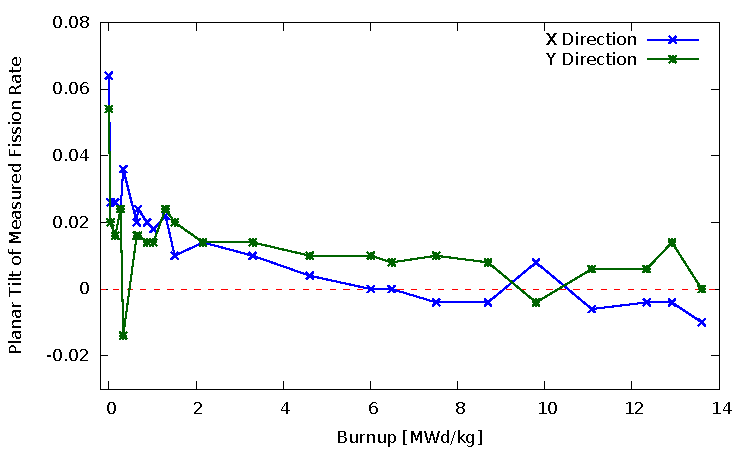
\includegraphics[width = 4.5 in]{figures/tilts_cyc1.pdf}
\caption{Magnitude of x and y tilts vs burnup for cycle 1.}
\label{fig:tilts_cyc1}
\end{figure}

\begin{figure}[!htb]
\centering
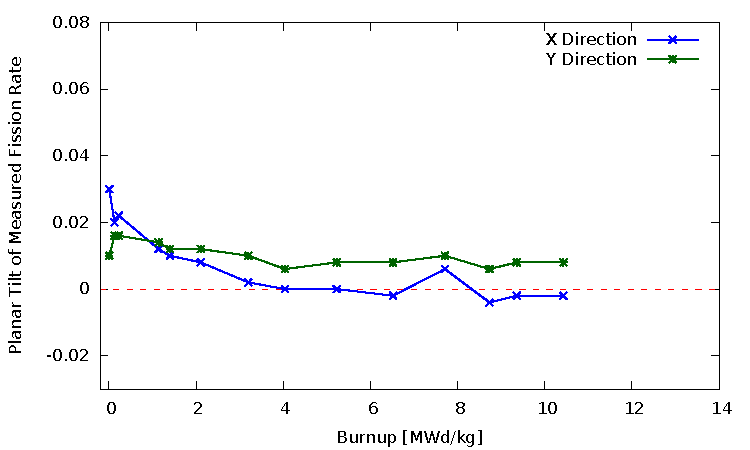
\includegraphics[width = 4.5 in]{figures/tilts_cyc2.pdf}
\caption{Magnitude of x and y tilts vs burnup for cycle 2.}
\label{fig:tilts_cyc2}
\end{figure}

\subsubsection{Initial Gap Test to Mimic Tilt in BEAVRS Data}\label{sec:init_gap_test}

A 0.5 cm water gap can be modeled in SIMULATE between the fuel assemblies and the baffle in the southeast corner of the core. To illustrate the effect of an updated model which includes this water gap on overall modeling accuracy, a radial error map before and after the water gap inclusion at HZP is shown in Figures \ref{fig:tc_uq_error_hzp} and \ref{fig:tc_uq_error_water_gap} respectively\footnote{The radial error map shown in Figure \ref{fig:tc_uq_error_water_gap} after adding a 0.5 cm water gap differs slightly from the one found in Sykora's Master's thesis because of updated BEAVRS specifications since the publishing of his findings. Further discrepancies also arise due to the fact that the SIMULATE-3 nodal diffusion solution was used instead of the CASMO-5 MxN full-core transport solution used by Sykora.}. While the core-wide RMS reduces dramatically, this simple water gap model does not wholly explain the cause of the tilt in BEAVRS data. A major reason for this is that the addition of the water gap induces an exponential tilt which helps reduce the errors on the periphery of the core but still adds significant errors in the core center, where a linear tilt is more suitable than an exponential one. Thus, accounting for varying water gaps throughout the core and not just at the edge will allow for tuning of the water gap to compensate for this phenomenon. Furthermore, Sykora finds that keeping a fixed water gap through depletion results in higher errors due to the resulting exponential tilt over-correcting the real tilt in BEAVRS data \cite{sykora_ms}. This suggests that the gap must vanish or reduce with burnup. A key element in tilt-correction uncertainty quantification therefore is to introduce more degrees of freedom in water gap distribution to reduce RMS and to match the BEAVRS radial map more closely to simulated results. This approach will be pursued in Section \ref{sec:tc_uq_method}. 

\definecolor{Dfourteencolor}{rgb}{0.8,0.265346832758,0.16}
\definecolor{Ntwocolor}{rgb}{0.455339342104,0.8,0.16}
\definecolor{Gsevencolor}{rgb}{1,1,1}
\definecolor{Gsixcolor}{rgb}{1,1,1}
\definecolor{Gfivecolor}{rgb}{0.8,0.746776945825,0.16}
\definecolor{Gfourcolor}{rgb}{1,1,1}
\definecolor{Gthreecolor}{rgb}{1,1,1}
\definecolor{Gtwocolor}{rgb}{1,1,1}
\definecolor{Gonecolor}{rgb}{1,1,1}
\definecolor{Nfourcolor}{rgb}{0.517065402164,0.8,0.16}
\definecolor{Kfourteencolor}{rgb}{1,1,1}
\definecolor{Gninecolor}{rgb}{0.8,0.665425987679,0.16}
\definecolor{Geightcolor}{rgb}{1,1,1}
\definecolor{Nsixcolor}{rgb}{0.52738144858,0.8,0.16}
\definecolor{Nsevencolor}{rgb}{1,1,1}
\definecolor{Rfivecolor}{rgb}{1,1,1}
\definecolor{Rsixcolor}{rgb}{0.16,0.8,0.16}
\definecolor{Rsevencolor}{rgb}{1,1,1}
\definecolor{Reightcolor}{rgb}{0.191958963693,0.8,0.16}
\definecolor{Rninecolor}{rgb}{1,1,1}
\definecolor{Jeightcolor}{rgb}{0.8,0.77610286567,0.16}
\definecolor{Jninecolor}{rgb}{1,1,1}
\definecolor{Jfourcolor}{rgb}{1,1,1}
\definecolor{Jfivecolor}{rgb}{1,1,1}
\definecolor{Jsixcolor}{rgb}{1,1,1}
\definecolor{Jsevencolor}{rgb}{0.8,0.706731660025,0.16}
\definecolor{Jonecolor}{rgb}{0.42559002141,0.8,0.16}
\definecolor{Jtwocolor}{rgb}{1,1,1}
\definecolor{Jthreecolor}{rgb}{1,1,1}
\definecolor{Bfourcolor}{rgb}{1,1,1}
\definecolor{Bfivecolor}{rgb}{1,1,1}
\definecolor{Bsixcolor}{rgb}{0.78897844219,0.8,0.16}
\definecolor{Bsevencolor}{rgb}{1,1,1}
\definecolor{Bthreecolor}{rgb}{0.79398702986,0.8,0.16}
\definecolor{Ksevencolor}{rgb}{1,1,1}
\definecolor{Beightcolor}{rgb}{0.8,0.655948849668,0.16}
\definecolor{Bninecolor}{rgb}{1,1,1}
\definecolor{Ksixcolor}{rgb}{0.753401079491,0.8,0.16}
\definecolor{Nfivecolor}{rgb}{1,1,1}
\definecolor{Kfivecolor}{rgb}{1,1,1}
\definecolor{Lfourteencolor}{rgb}{1,1,1}
\definecolor{Lfifteencolor}{rgb}{0.8,0.718451154587,0.16}
\definecolor{Kfourcolor}{rgb}{1,1,1}
\definecolor{Ltencolor}{rgb}{0.773277476893,0.8,0.16}
\definecolor{Lelevencolor}{rgb}{0.8,0.63486461458,0.16}
\definecolor{Ltwelvecolor}{rgb}{1,1,1}
\definecolor{Lthirteencolor}{rgb}{0.8,0.725819417854,0.16}
\definecolor{Mfivecolor}{rgb}{1,1,1}
\definecolor{Mfourcolor}{rgb}{1,1,1}
\definecolor{Msevencolor}{rgb}{0.61480772461,0.8,0.16}
\definecolor{Msixcolor}{rgb}{1,1,1}
\definecolor{Mthreecolor}{rgb}{1,1,1}
\definecolor{Mtwocolor}{rgb}{1,1,1}
\definecolor{Mninecolor}{rgb}{1,1,1}
\definecolor{Meightcolor}{rgb}{1,1,1}
\definecolor{Rtencolor}{rgb}{1,1,1}
\definecolor{Relevencolor}{rgb}{0.658159123195,0.8,0.16}
\definecolor{Mfourteencolor}{rgb}{1,1,1}
\definecolor{Ptencolor}{rgb}{1,1,1}
\definecolor{Pelevencolor}{rgb}{1,1,1}
\definecolor{Ptwelvecolor}{rgb}{1,1,1}
\definecolor{Pthirteencolor}{rgb}{1,1,1}
\definecolor{Eninecolor}{rgb}{0.8,0.553221357547,0.16}
\definecolor{Eeightcolor}{rgb}{1,1,1}
\definecolor{Efivecolor}{rgb}{0.8,0.69668967433,0.16}
\definecolor{Efourcolor}{rgb}{1,1,1}
\definecolor{Esevencolor}{rgb}{1,1,1}
\definecolor{Esixcolor}{rgb}{1,1,1}
\definecolor{Eonecolor}{rgb}{1,1,1}
\definecolor{Peightcolor}{rgb}{1,1,1}
\definecolor{Ethreecolor}{rgb}{1,1,1}
\definecolor{Etwocolor}{rgb}{1,1,1}
\definecolor{Pthreecolor}{rgb}{1,1,1}
\definecolor{Pninecolor}{rgb}{0.463728913731,0.8,0.16}
\definecolor{Psixcolor}{rgb}{1,1,1}
\definecolor{Psevencolor}{rgb}{1,1,1}
\definecolor{Pfourcolor}{rgb}{0.452199094545,0.8,0.16}
\definecolor{Pfivecolor}{rgb}{1,1,1}
\definecolor{Htencolor}{rgb}{1,1,1}
\definecolor{Helevencolor}{rgb}{0.8,0.575542078177,0.16}
\definecolor{Htwelvecolor}{rgb}{1,1,1}
\definecolor{Hthirteencolor}{rgb}{0.8,0.560020020072,0.16}
\definecolor{Hfourteencolor}{rgb}{1,1,1}
\definecolor{Hfifteencolor}{rgb}{0.8,0.699723915021,0.16}
\definecolor{Ftwelvecolor}{rgb}{1,1,1}
\definecolor{Fthirteencolor}{rgb}{1,1,1}
\definecolor{Ftencolor}{rgb}{1,1,1}
\definecolor{Felevencolor}{rgb}{1,1,1}
\definecolor{Ffourteencolor}{rgb}{0.8,0.38245646751,0.16}
\definecolor{Ffifteencolor}{rgb}{1,1,1}
\definecolor{Ntwelvecolor}{rgb}{1,1,1}
\definecolor{Nthirteencolor}{rgb}{0.711549268258,0.8,0.16}
\definecolor{Heightcolor}{rgb}{1,1,1}
\definecolor{Nelevencolor}{rgb}{1,1,1}
\definecolor{Nfourteencolor}{rgb}{0.8,0.729037702287,0.16}
\definecolor{Htwocolor}{rgb}{0.665522940493,0.8,0.16}
\definecolor{Hthreecolor}{rgb}{0.587616200245,0.8,0.16}
\definecolor{Honecolor}{rgb}{1,1,1}
\definecolor{Hsixcolor}{rgb}{0.8,0.775509786637,0.16}
\definecolor{Hsevencolor}{rgb}{1,1,1}
\definecolor{Hfourcolor}{rgb}{0.747938120349,0.8,0.16}
\definecolor{Hfivecolor}{rgb}{1,1,1}
\definecolor{Kthirteencolor}{rgb}{1,1,1}
\definecolor{Ktwelvecolor}{rgb}{0.8,0.604277470963,0.16}
\definecolor{Kelevencolor}{rgb}{1,1,1}
\definecolor{Ktencolor}{rgb}{1,1,1}
\definecolor{Dtencolor}{rgb}{0.8,0.356450335132,0.16}
\definecolor{Delevencolor}{rgb}{1,1,1}
\definecolor{Dtwelvecolor}{rgb}{0.8,0.398250061786,0.16}
\definecolor{Dthirteencolor}{rgb}{1,1,1}
\definecolor{Kthreecolor}{rgb}{1,1,1}
\definecolor{Ktwocolor}{rgb}{0.499923245527,0.8,0.16}
\definecolor{Konecolor}{rgb}{1,1,1}
\definecolor{Btwelvecolor}{rgb}{1,1,1}
\definecolor{Bthirteencolor}{rgb}{0.8,0.16,0.16}
\definecolor{Btencolor}{rgb}{1,1,1}
\definecolor{Belevencolor}{rgb}{1,1,1}
\definecolor{Kninecolor}{rgb}{1,1,1}
\definecolor{Keightcolor}{rgb}{1,1,1}
\definecolor{Nthreecolor}{rgb}{1,1,1}
\definecolor{Cninecolor}{rgb}{1,1,1}
\definecolor{Ceightcolor}{rgb}{0.8,0.650282411305,0.16}
\definecolor{Cthreecolor}{rgb}{1,1,1}
\definecolor{Ctwocolor}{rgb}{1,1,1}
\definecolor{Kfifteencolor}{rgb}{1,1,1}
\definecolor{Jfifteencolor}{rgb}{1,1,1}
\definecolor{Csevencolor}{rgb}{0.8,0.687030312523,0.16}
\definecolor{Csixcolor}{rgb}{1,1,1}
\definecolor{Cfivecolor}{rgb}{0.8,0.793039247613,0.16}
\definecolor{Cfourcolor}{rgb}{1,1,1}
\definecolor{Etwelvecolor}{rgb}{1,1,1}
\definecolor{Ntencolor}{rgb}{1,1,1}
\definecolor{Neightcolor}{rgb}{0.592745400538,0.8,0.16}
\definecolor{Nninecolor}{rgb}{1,1,1}
\definecolor{Hninecolor}{rgb}{1,1,1}
\definecolor{Gfifteencolor}{rgb}{1,1,1}
\definecolor{Gfourteencolor}{rgb}{1,1,1}
\definecolor{Gthirteencolor}{rgb}{1,1,1}
\definecolor{Gtwelvecolor}{rgb}{0.8,0.440331870439,0.16}
\definecolor{Gelevencolor}{rgb}{1,1,1}
\definecolor{Gtencolor}{rgb}{1,1,1}
\definecolor{Fonecolor}{rgb}{0.390109195085,0.8,0.16}
\definecolor{Ftwocolor}{rgb}{1,1,1}
\definecolor{Fthreecolor}{rgb}{0.774581059212,0.8,0.16}
\definecolor{Ffourcolor}{rgb}{1,1,1}
\definecolor{Ffivecolor}{rgb}{1,1,1}
\definecolor{Fsixcolor}{rgb}{1,1,1}
\definecolor{Fsevencolor}{rgb}{0.8,0.798517098201,0.16}
\definecolor{Feightcolor}{rgb}{0.8,0.566404090074,0.16}
\definecolor{Fninecolor}{rgb}{1,1,1}
\definecolor{Jthirteencolor}{rgb}{1,1,1}
\definecolor{Melevencolor}{rgb}{1,1,1}
\definecolor{Mtencolor}{rgb}{1,1,1}
\definecolor{Mthirteencolor}{rgb}{1,1,1}
\definecolor{Mtwelvecolor}{rgb}{1,1,1}
\definecolor{Jtencolor}{rgb}{0.8,0.648476246095,0.16}
\definecolor{Jelevencolor}{rgb}{1,1,1}
\definecolor{Eelevencolor}{rgb}{0.8,0.395393925047,0.16}
\definecolor{Etencolor}{rgb}{1,1,1}
\definecolor{Ethirteencolor}{rgb}{1,1,1}
\definecolor{Jfourteencolor}{rgb}{0.8,0.662011345315,0.16}
\definecolor{Efifteencolor}{rgb}{1,1,1}
\definecolor{Efourteencolor}{rgb}{1,1,1}
\definecolor{Cthirteencolor}{rgb}{1,1,1}
\definecolor{Ctwelvecolor}{rgb}{1,1,1}
\definecolor{Celevencolor}{rgb}{1,1,1}
\definecolor{Ctencolor}{rgb}{1,1,1}
\definecolor{Cfourteencolor}{rgb}{1,1,1}
\definecolor{Aelevencolor}{rgb}{0.8,0.497860119121,0.16}
\definecolor{Atencolor}{rgb}{1,1,1}
\definecolor{Afivecolor}{rgb}{1,1,1}
\definecolor{Asevencolor}{rgb}{1,1,1}
\definecolor{Asixcolor}{rgb}{1,1,1}
\definecolor{Aninecolor}{rgb}{0.8,0.74471275811,0.16}
\definecolor{Aeightcolor}{rgb}{1,1,1}
\definecolor{Jtwelvecolor}{rgb}{1,1,1}
\definecolor{Lsixcolor}{rgb}{1,1,1}
\definecolor{Lsevencolor}{rgb}{1,1,1}
\definecolor{Lfourcolor}{rgb}{1,1,1}
\definecolor{Lfivecolor}{rgb}{0.56032709494,0.8,0.16}
\definecolor{Ltwocolor}{rgb}{1,1,1}
\definecolor{Lthreecolor}{rgb}{1,1,1}
\definecolor{Lonecolor}{rgb}{1,1,1}
\definecolor{Leightcolor}{rgb}{0.762674204472,0.8,0.16}
\definecolor{Lninecolor}{rgb}{1,1,1}
\definecolor{Deightcolor}{rgb}{0.8,0.597477114162,0.16}
\definecolor{Dninecolor}{rgb}{1,1,1}
\definecolor{Dsixcolor}{rgb}{1,1,1}
\definecolor{Dsevencolor}{rgb}{1,1,1}
\definecolor{Dfourcolor}{rgb}{1,1,1}
\definecolor{Dfivecolor}{rgb}{1,1,1}
\definecolor{Dtwocolor}{rgb}{1,1,1}
\definecolor{Dthreecolor}{rgb}{0.765542246483,0.8,0.16}

\begin{figure}[!htb]
    \centering
    
    % these dimensions are determined in arrow_dimms.ods

    \def\scale{1.6}

    \def\latWidth{0.2673473684*\scale}
    
    \def\RPVOR{3*\scale}
    \def\rectW{0.75*\scale}
    \def\RPVIR{2.7315789474*\scale}
    \def\BarrelIR{2.3368421053*\scale}
    \def\BarrelOR{2.4078947368*\scale}
    \def\ShieldIR{2.4223787816*\scale}
    \def\ShieldOR{2.5067965189*\scale}
    \def\LinerIR{2.7246166598*\scale}

    \def\bafCIRx{0.9357157895*\scale}
    \def\bafCIRy{2.0051052632*\scale}
    \def\bafCORx{0.9633473684*\scale}
    \def\bafCORy{2.0327368421*\scale}
    \def\bafMIRx{1.7377578947*\scale}
    \def\bafMIRy{1.4704105263*\scale}
    \def\bafMORx{1.7653894737*\scale}
    \def\bafMORy{1.4980421053*\scale}
    
    \tikzset{Assembly/.style={
        inner sep=0pt,
        text width=\latWidth in,
        minimum size=\latWidth in,
        draw=black,
        align=center
        }
    }
    
    \def\tkzRPV{(0,0) circle (\RPVIR) (0,0) circle (\RPVOR)}
    \def\tkzLiner{(0,0) circle (\LinerIR) (0,0) circle (\RPVIR)}
    \def\tkzBarrel{(0,0) circle (\BarrelIR) (0,0) circle (\BarrelOR)}
    \def\tkzShields{(0,0) circle (\ShieldIR) (0,0) circle (\ShieldOR)}
    
    \def\tkzBaffCOR{(-\bafCORx, -\bafCORy) rectangle (\bafCORx, \bafCORy)}
    \def\tkzBaffCIR{(-\bafCIRx, -\bafCIRy) rectangle (\bafCIRx, \bafCIRy)} 
    \def\tkzBaffMOR{(-\bafMORx, -\bafMORy) rectangle (\bafMORx, \bafMORy)}
    \def\tkzBaffMIR{(-\bafMIRx, -\bafMIRy) rectangle (\bafMIRx, \bafMIRy) }
    \def\tkzBaffleC{ \tkzBaffCIR \tkzBaffCOR }
    \def\tkzBaffleM{ \tkzBaffMIR \tkzBaffMOR }

    \def\tkzBaffCClip{\tkzBaffCIR (-\RPVOR, -\RPVOR) rectangle (\RPVOR, \RPVOR)}
    \def\tkzBaffMClip{\tkzBaffMIR (-\RPVOR, -\RPVOR) rectangle (\RPVOR, \RPVOR)}

    \def\highenr{blue!50}
    \def\midenr{yellow!50}
    \def\lowenr{red!50}

    \scalebox{0.6}{

      \begin{tikzpicture}[x=1in,y=1in]
      \fontfamily{mdbch}\selectfont
        % draw RPV, barrel, and shield panels
        
        \path[fill=black!90!white,even odd rule] \tkzRPV;
        \path[fill=black,even odd rule] \tkzLiner;
        \path[fill=black,even odd rule] \tkzBarrel;
        \begin{scope}
          \clip (0,0) -- +(61:\RPVOR) arc (61:29:\RPVOR) --
                (0,0) -- +(151:\RPVOR) arc (151:119:\RPVOR) -- 
                (0,0) -- +(241:\RPVOR) arc (241:209:\RPVOR) -- 
                (0,0) -- +(331:\RPVOR) arc (331:299:\RPVOR) -- cycle;
          \path[fill=black,even odd rule] \tkzShields;
        \end{scope}

        % draw baffle north/south
        
        \begin{scope}[even odd rule]
          \clip[rotate=90] \tkzBaffMClip;
          \path[fill=black] \tkzBaffleC;
        \end{scope}
        \begin{scope}[even odd rule]
          \clip \tkzBaffCClip;
          \clip \tkzBaffMClip;
          \path[fill=black, rotate=90] \tkzBaffleM;
        \end{scope}
        
        % draw baffle east/west
        
        \begin{scope}[rotate=90]
          \begin{scope}[even odd rule]
            \clip[rotate=90] \tkzBaffMClip;
            \path[fill=black] \tkzBaffleC;
          \end{scope}
          \begin{scope}[even odd rule]
            \clip \tkzBaffCClip;
            \clip \tkzBaffMClip;
            \path[fill=black, rotate=90] \tkzBaffleM;
          \end{scope}
        \end{scope}
        
        % draw assembly row/column headers
        
        \draw[red, thick] ($(-7*\latWidth,0.4*\RPVOR/\latWidth*\latWidth)$) node[above, anchor=south] {R} -- ($(-7*\latWidth,4*\latWidth)$);
        \draw[red, thick] ($(-6*\latWidth,0.4*\RPVOR/\latWidth*\latWidth)$) node[above, anchor=south] {P} -- ($(-6*\latWidth,6*\latWidth)$);
        \draw[red, thick] ($(-5*\latWidth,0.4*\RPVOR/\latWidth*\latWidth)$) node[above, anchor=south] {N} -- ($(-5*\latWidth,7*\latWidth)$);
        \draw[red, thick] ($(-4*\latWidth,0.4*\RPVOR/\latWidth*\latWidth)$) node[above, anchor=south] {M} -- ($(-4*\latWidth,7*\latWidth)$);
        \draw[red, thick] ($(-3*\latWidth,0.4*\RPVOR/\latWidth*\latWidth)$) node[above, anchor=south] {L} -- ($(-3*\latWidth,8*\latWidth)$);
        \draw[red, thick] ($(-2*\latWidth,0.4*\RPVOR/\latWidth*\latWidth)$) node[above, anchor=south] {K} -- ($(-2*\latWidth,8*\latWidth)$);
        \draw[red, thick] ($(-1*\latWidth,0.4*\RPVOR/\latWidth*\latWidth)$) node[above, anchor=south] {J} -- ($(-1*\latWidth,8*\latWidth)$);
        \draw[red, thick] ($(-0*\latWidth,0.4*\RPVOR/\latWidth*\latWidth)$) node[above, anchor=south] {H} -- ($(-0*\latWidth,8*\latWidth)$);
        \draw[red, thick] ($(1*\latWidth,0.4*\RPVOR/\latWidth*\latWidth)$) node[above, anchor=south] {G} -- ($(1*\latWidth,8*\latWidth)$);
        \draw[red, thick] ($(2*\latWidth,0.4*\RPVOR/\latWidth*\latWidth)$) node[above, anchor=south] {F} -- ($(2*\latWidth,8*\latWidth)$);
        \draw[red, thick] ($(3*\latWidth,0.4*\RPVOR/\latWidth*\latWidth)$) node[above, anchor=south] {E} -- ($(3*\latWidth,8*\latWidth)$);
        \draw[red, thick] ($(4*\latWidth,0.4*\RPVOR/\latWidth*\latWidth)$) node[above, anchor=south] {D} -- ($(4*\latWidth,7*\latWidth)$);
        \draw[red, thick] ($(5*\latWidth,0.4*\RPVOR/\latWidth*\latWidth)$) node[above, anchor=south] {C} -- ($(5*\latWidth,7*\latWidth)$);
        \draw[red, thick] ($(6*\latWidth,0.4*\RPVOR/\latWidth*\latWidth)$) node[above, anchor=south] {B} -- ($(6*\latWidth,6*\latWidth)$);
        \draw[red, thick] ($(7*\latWidth,0.4*\RPVOR/\latWidth*\latWidth)$) node[above, anchor=south] {A} -- ($(7*\latWidth,4*\latWidth)$);
        
        \begin{scope}[rotate=90]
          \draw[red, thick] ($(-7*\latWidth,0.4*\RPVOR/\latWidth*\latWidth)$) node[left, anchor=east] {15} -- ($(-7*\latWidth,4*\latWidth)$);
          \draw[red, thick] ($(-6*\latWidth,0.4*\RPVOR/\latWidth*\latWidth)$) node[left, anchor=east] {14} -- ($(-6*\latWidth,6*\latWidth)$);
          \draw[red, thick] ($(-5*\latWidth,0.4*\RPVOR/\latWidth*\latWidth)$) node[left, anchor=east] {13} -- ($(-5*\latWidth,7*\latWidth)$);
          \draw[red, thick] ($(-4*\latWidth,0.4*\RPVOR/\latWidth*\latWidth)$) node[left, anchor=east] {12} -- ($(-4*\latWidth,7*\latWidth)$);
          \draw[red, thick] ($(-3*\latWidth,0.4*\RPVOR/\latWidth*\latWidth)$) node[left, anchor=east] {11} -- ($(-3*\latWidth,8*\latWidth)$);
          \draw[red, thick] ($(-2*\latWidth,0.4*\RPVOR/\latWidth*\latWidth)$) node[left, anchor=east] {10} -- ($(-2*\latWidth,8*\latWidth)$);
          \draw[red, thick] ($(-1*\latWidth,0.4*\RPVOR/\latWidth*\latWidth)$) node[left, anchor=east] {9} -- ($(-1*\latWidth,8*\latWidth)$);
          \draw[red, thick] ($(-0*\latWidth,0.4*\RPVOR/\latWidth*\latWidth)$) node[left, anchor=east] {8} -- ($(-0*\latWidth,8*\latWidth)$);
          \draw[red, thick] ($(1*\latWidth,0.4*\RPVOR/\latWidth*\latWidth)$) node[left, anchor=east] {7} -- ($(1*\latWidth,8*\latWidth)$);
          \draw[red, thick] ($(2*\latWidth,0.4*\RPVOR/\latWidth*\latWidth)$) node[left, anchor=east] {6} -- ($(2*\latWidth,8*\latWidth)$);
          \draw[red, thick] ($(3*\latWidth,0.4*\RPVOR/\latWidth*\latWidth)$) node[left, anchor=east] {5} -- ($(3*\latWidth,8*\latWidth)$);
          \draw[red, thick] ($(4*\latWidth,0.4*\RPVOR/\latWidth*\latWidth)$) node[left, anchor=east] {4} -- ($(4*\latWidth,7*\latWidth)$);
          \draw[red, thick] ($(5*\latWidth,0.4*\RPVOR/\latWidth*\latWidth)$) node[left, anchor=east] {3} -- ($(5*\latWidth,7*\latWidth)$);
          \draw[red, thick] ($(6*\latWidth,0.4*\RPVOR/\latWidth*\latWidth)$) node[left, anchor=east] {2} -- ($(6*\latWidth,6*\latWidth)$);
          \draw[red, thick] ($(7*\latWidth,0.4*\RPVOR/\latWidth*\latWidth)$) node[left, anchor=east] {1} -- ($(7*\latWidth,4*\latWidth)$);
        \end{scope}
        
        
        % draw fuel assembly nodes
        
        \node [Assembly, fill=Lonecolor] at ($(-3*\latWidth,7*\latWidth)$) {}; % L1
        \node [Assembly, fill=Konecolor] at ($(-2*\latWidth,7*\latWidth)$) {}; % K1
        \node [Assembly, fill=Jonecolor] at ($(-1*\latWidth,7*\latWidth)$) {\scriptsize{-0.085}}; % J1
        \node [Assembly, fill=Honecolor] at ($(-0*\latWidth,7*\latWidth)$) {}; % H1
        \node [Assembly, fill=Gonecolor] at ($( 1*\latWidth,7*\latWidth)$) {}; % G1
        \node [Assembly, fill=Fonecolor] at ($( 2*\latWidth,7*\latWidth)$) {\scriptsize{-0.093}}; % F1
        \node [Assembly, fill=Eonecolor] at ($( 3*\latWidth,7*\latWidth)$) {}; % E1

        \node [Assembly, fill=Ntwocolor] at ($(-5*\latWidth,6*\latWidth)$) {\scriptsize{-0.079}}; % N2
        \node [Assembly, fill=Mtwocolor] at ($(-4*\latWidth,6*\latWidth)$) {}; % M2
        \node [Assembly, fill=Ltwocolor] at ($(-3*\latWidth,6*\latWidth)$) {}; % L2
        \node [Assembly, fill=Ktwocolor] at ($(-2*\latWidth,6*\latWidth)$) {\scriptsize{-0.070}}; % K2
        \node [Assembly, fill=Jtwocolor] at ($(-1*\latWidth,6*\latWidth)$) {}; % J2
        \node [Assembly, fill=Htwocolor] at ($(-0*\latWidth,6*\latWidth)$) {\scriptsize{-0.036}}; % H2
        \node [Assembly, fill=Gtwocolor] at ($( 1*\latWidth,6*\latWidth)$) {}; % G2
        \node [Assembly, fill=Ftwocolor] at ($( 2*\latWidth,6*\latWidth)$) {}; % F2
        \node [Assembly, fill=Etwocolor] at ($( 3*\latWidth,6*\latWidth)$) {}; % E2
        \node [Assembly, fill=Dtwocolor] at ($( 4*\latWidth,6*\latWidth)$) {}; % D2
        \node [Assembly, fill=Ctwocolor] at ($( 5*\latWidth,6*\latWidth)$) {}; % C2

        \node [Assembly, fill=Pthreecolor] at ($(-6*\latWidth,5*\latWidth)$) {}; % P3
        \node [Assembly, fill=Nthreecolor] at ($(-5*\latWidth,5*\latWidth)$) {}; % N3
        \node [Assembly, fill=Mthreecolor] at ($(-4*\latWidth,5*\latWidth)$) {}; % M3
        \node [Assembly, fill=Lthreecolor] at ($(-3*\latWidth,5*\latWidth)$) {}; % L3
        \node [Assembly, fill=Kthreecolor] at ($(-2*\latWidth,5*\latWidth)$) {}; % K3
        \node [Assembly, fill=Jthreecolor] at ($(-1*\latWidth,5*\latWidth)$) {}; % J3
        \node [Assembly, fill=Hthreecolor] at ($(-0*\latWidth,5*\latWidth)$) {\scriptsize{-0.052}}; % H3
        \node [Assembly, fill=Gthreecolor] at ($( 1*\latWidth,5*\latWidth)$) {}; % G3
        \node [Assembly, fill=Fthreecolor] at ($( 2*\latWidth,5*\latWidth)$) {\scriptsize{-0.014}}; % F3
        \node [Assembly, fill=Ethreecolor] at ($( 3*\latWidth,5*\latWidth)$) {}; % E3
        \node [Assembly, fill=Dthreecolor] at ($( 4*\latWidth,5*\latWidth)$) {\scriptsize{-0.016}}; % D3
        \node [Assembly, fill=Cthreecolor] at ($( 5*\latWidth,5*\latWidth)$) {}; % C3
        \node [Assembly, fill=Bthreecolor] at ($( 6*\latWidth,5*\latWidth)$) {\scriptsize{-0.010}}; % B3

        \node [Assembly, fill=Pfourcolor] at ($(-6*\latWidth,4*\latWidth)$) {\scriptsize{-0.080}}; % P4
        \node [Assembly, fill=Nfourcolor] at ($(-5*\latWidth,4*\latWidth)$) {\scriptsize{-0.067}}; % N4
        \node [Assembly, fill=Mfourcolor] at ($(-4*\latWidth,4*\latWidth)$) {}; % M4
        \node [Assembly, fill=Lfourcolor] at ($(-3*\latWidth,4*\latWidth)$) {}; % L4
        \node [Assembly, fill=Kfourcolor] at ($(-2*\latWidth,4*\latWidth)$) {}; % K4
        \node [Assembly, fill=Jfourcolor] at ($(-1*\latWidth,4*\latWidth)$) {}; % J4
        \node [Assembly, fill=Hfourcolor] at ($(-0*\latWidth,4*\latWidth)$) {\scriptsize{-0.020}}; % H4
        \node [Assembly, fill=Gfourcolor] at ($( 1*\latWidth,4*\latWidth)$) {}; % G4
        \node [Assembly, fill=Ffourcolor] at ($( 2*\latWidth,4*\latWidth)$) {}; % F4
        \node [Assembly, fill=Efourcolor] at ($( 3*\latWidth,4*\latWidth)$) {}; % E4
        \node [Assembly, fill=Dfourcolor] at ($( 4*\latWidth,4*\latWidth)$) {}; % D4
        \node [Assembly, fill=Cfourcolor] at ($( 5*\latWidth,4*\latWidth)$) {}; % C4
        \node [Assembly, fill=Bfourcolor] at ($( 6*\latWidth,4*\latWidth)$) {}; % B4

        \node [Assembly, fill=Rfivecolor] at ($(-7*\latWidth,3*\latWidth)$) {}; % R5
        \node [Assembly, fill=Pfivecolor] at ($(-6*\latWidth,3*\latWidth)$) {}; % P5
        \node [Assembly, fill=Nfivecolor] at ($(-5*\latWidth,3*\latWidth)$) {}; % N5
        \node [Assembly, fill=Mfivecolor] at ($(-4*\latWidth,3*\latWidth)$) {}; % M5
        \node [Assembly, fill=Lfivecolor] at ($(-3*\latWidth,3*\latWidth)$) {\scriptsize{-0.058}}; % L5
        \node [Assembly, fill=Kfivecolor] at ($(-2*\latWidth,3*\latWidth)$) {}; % K5
        \node [Assembly, fill=Jfivecolor] at ($(-1*\latWidth,3*\latWidth)$) {}; % J5
        \node [Assembly, fill=Hfivecolor] at ($(-0*\latWidth,3*\latWidth)$) {}; % H5
        \node [Assembly, fill=Gfivecolor] at ($( 1*\latWidth,3*\latWidth)$) {\scriptsize{0.002}}; % G5
        \node [Assembly, fill=Ffivecolor] at ($( 2*\latWidth,3*\latWidth)$) {}; % F5
        \node [Assembly, fill=Efivecolor] at ($( 3*\latWidth,3*\latWidth)$) {\scriptsize{0.012}}; % E5
        \node [Assembly, fill=Dfivecolor] at ($( 4*\latWidth,3*\latWidth)$) {}; % D5
        \node [Assembly, fill=Cfivecolor] at ($( 5*\latWidth,3*\latWidth)$) {\scriptsize{-0.007}}; % C5
        \node [Assembly, fill=Bfivecolor] at ($( 6*\latWidth,3*\latWidth)$) {}; % B5
        \node [Assembly, fill=Afivecolor] at ($( 7*\latWidth,3*\latWidth)$) {}; % A5

        \node [Assembly, fill=Rsixcolor] at ($(-7*\latWidth,2*\latWidth)$) {\scriptsize{-0.140}}; % R6
        \node [Assembly, fill=Psixcolor] at ($(-6*\latWidth,2*\latWidth)$) {}; % P6
        \node [Assembly, fill=Nsixcolor] at ($(-5*\latWidth,2*\latWidth)$) {\scriptsize{-0.065}}; % N6
        \node [Assembly, fill=Msixcolor] at ($(-4*\latWidth,2*\latWidth)$) {}; % M6
        \node [Assembly, fill=Lsixcolor] at ($(-3*\latWidth,2*\latWidth)$) {}; % L6
        \node [Assembly, fill=Ksixcolor] at ($(-2*\latWidth,2*\latWidth)$) {\scriptsize{-0.018}}; % K6
        \node [Assembly, fill=Jsixcolor] at ($(-1*\latWidth,2*\latWidth)$) {}; % J6
        \node [Assembly, fill=Hsixcolor] at ($(-0*\latWidth,2*\latWidth)$) {\scriptsize{-0.004}}; % H6
        \node [Assembly, fill=Gsixcolor] at ($( 1*\latWidth,2*\latWidth)$) {}; % G6
        \node [Assembly, fill=Fsixcolor] at ($( 2*\latWidth,2*\latWidth)$) {}; % F6
        \node [Assembly, fill=Esixcolor] at ($( 3*\latWidth,2*\latWidth)$) {}; % E6
        \node [Assembly, fill=Dsixcolor] at ($( 4*\latWidth,2*\latWidth)$) {}; % D6
        \node [Assembly, fill=Csixcolor] at ($( 5*\latWidth,2*\latWidth)$) {}; % C6
        \node [Assembly, fill=Bsixcolor] at ($( 6*\latWidth,2*\latWidth)$) {\scriptsize{-0.011}}; % B6
        \node [Assembly, fill=Asixcolor] at ($( 7*\latWidth,2*\latWidth)$) {}; % A6

        \node [Assembly, fill=Rsevencolor] at ($(-7*\latWidth,1*\latWidth)$) {}; % R7
        \node [Assembly, fill=Psevencolor] at ($(-6*\latWidth,1*\latWidth)$) {}; % P7
        \node [Assembly, fill=Nsevencolor] at ($(-5*\latWidth,1*\latWidth)$) {}; % N7
        \node [Assembly, fill=Msevencolor] at ($(-4*\latWidth,1*\latWidth)$) {\scriptsize{-0.047}}; % M7
        \node [Assembly, fill=Lsevencolor] at ($(-3*\latWidth,1*\latWidth)$) {}; % L7
        \node [Assembly, fill=Ksevencolor] at ($(-2*\latWidth,1*\latWidth)$) {}; % K7
        \node [Assembly, fill=Jsevencolor] at ($(-1*\latWidth,1*\latWidth)$) {\scriptsize{0.010}}; % J7
        \node [Assembly, fill=Hsevencolor] at ($(-0*\latWidth,1*\latWidth)$) {}; % H7
        \node [Assembly, fill=Gsevencolor] at ($( 1*\latWidth,1*\latWidth)$) {}; % G7
        \node [Assembly, fill=Fsevencolor] at ($( 2*\latWidth,1*\latWidth)$) {\scriptsize{-0.009}}; % F7
        \node [Assembly, fill=Esevencolor] at ($( 3*\latWidth,1*\latWidth)$) {}; % E7
        \node [Assembly, fill=Dsevencolor] at ($( 4*\latWidth,1*\latWidth)$) {}; % D7
        \node [Assembly, fill=Csevencolor] at ($( 5*\latWidth,1*\latWidth)$) {\scriptsize{0.014}}; % C7
        \node [Assembly, fill=Bsevencolor] at ($( 6*\latWidth,1*\latWidth)$) {}; % B7
        \node [Assembly, fill=Asevencolor] at ($( 7*\latWidth,1*\latWidth)$) {}; % A7

        \node [Assembly, fill=Reightcolor] at ($(-7*\latWidth,0*\latWidth)$) {\scriptsize{-0.133}}; % R8
        \node [Assembly, fill=Peightcolor] at ($(-6*\latWidth,0*\latWidth)$) {}; % P8
        \node [Assembly, fill=Neightcolor] at ($(-5*\latWidth,0*\latWidth)$) {\scriptsize{-0.051}}; % N8
        \node [Assembly, fill=Meightcolor] at ($(-4*\latWidth,0*\latWidth)$) {}; % M8
        \node [Assembly, fill=Leightcolor] at ($(-3*\latWidth,0*\latWidth)$) {\scriptsize{-0.017}}; % L8
        \node [Assembly, fill=Keightcolor] at ($(-2*\latWidth,0*\latWidth)$) {}; % K8
        \node [Assembly, fill=Jeightcolor] at ($(-1*\latWidth,0*\latWidth)$) {\scriptsize{-0.004}}; % J8
        \node [Assembly, fill=Heightcolor] at ($(-0*\latWidth,0*\latWidth)$) {}; % H8
        \node [Assembly, fill=Geightcolor] at ($( 1*\latWidth,0*\latWidth)$) {}; % G8
        \node [Assembly, fill=Feightcolor] at ($( 2*\latWidth,0*\latWidth)$) {\scriptsize{0.039}}; % F8
        \node [Assembly, fill=Eeightcolor] at ($( 3*\latWidth,0*\latWidth)$) {}; % E8
        \node [Assembly, fill=Deightcolor] at ($( 4*\latWidth,0*\latWidth)$) {\scriptsize{0.032}}; % D8
        \node [Assembly, fill=Ceightcolor] at ($( 5*\latWidth,0*\latWidth)$) {\scriptsize{0.022}}; % C8
        \node [Assembly, fill=Beightcolor] at ($( 6*\latWidth,0*\latWidth)$) {\scriptsize{0.021}}; % B8
        \node [Assembly, fill=Aeightcolor] at ($( 7*\latWidth,0*\latWidth)$) {}; % A8

        \node [Assembly, fill=Rninecolor] at ($(-7*\latWidth,-1*\latWidth)$) {}; % R9
        \node [Assembly, fill=Pninecolor] at ($(-6*\latWidth,-1*\latWidth)$) {\scriptsize{-0.078}}; % P9
        \node [Assembly, fill=Nninecolor] at ($(-5*\latWidth,-1*\latWidth)$) {}; % N9
        \node [Assembly, fill=Mninecolor] at ($(-4*\latWidth,-1*\latWidth)$) {}; % M9
        \node [Assembly, fill=Lninecolor] at ($(-3*\latWidth,-1*\latWidth)$) {}; % L9
        \node [Assembly, fill=Kninecolor] at ($(-2*\latWidth,-1*\latWidth)$) {}; % K9
        \node [Assembly, fill=Jninecolor] at ($(-1*\latWidth,-1*\latWidth)$) {}; % J9
        \node [Assembly, fill=Hninecolor] at ($(-0*\latWidth,-1*\latWidth)$) {}; % H9
        \node [Assembly, fill=Gninecolor] at ($( 1*\latWidth,-1*\latWidth)$) {\scriptsize{0.019}}; % G9
        \node [Assembly, fill=Fninecolor] at ($( 2*\latWidth,-1*\latWidth)$) {}; % F9
        \node [Assembly, fill=Eninecolor] at ($( 3*\latWidth,-1*\latWidth)$) {\scriptsize{0.042}}; % E9
        \node [Assembly, fill=Dninecolor] at ($( 4*\latWidth,-1*\latWidth)$) {}; % D9
        \node [Assembly, fill=Cninecolor] at ($( 5*\latWidth,-1*\latWidth)$) {}; % C9
        \node [Assembly, fill=Bninecolor] at ($( 6*\latWidth,-1*\latWidth)$) {}; % B9
        \node [Assembly, fill=Aninecolor] at ($( 7*\latWidth,-1*\latWidth)$) {\scriptsize{0.002}}; % A9

        \node [Assembly, fill=Rtencolor] at ($(-7*\latWidth,-2*\latWidth)$) {}; % R10
        \node [Assembly, fill=Ptencolor] at ($(-6*\latWidth,-2*\latWidth)$) {}; % P10
        \node [Assembly, fill=Ntencolor] at ($(-5*\latWidth,-2*\latWidth)$) {}; % N10
        \node [Assembly, fill=Mtencolor] at ($(-4*\latWidth,-2*\latWidth)$) {}; % M10
        \node [Assembly, fill=Ltencolor] at ($(-3*\latWidth,-2*\latWidth)$) {\scriptsize{-0.014}}; % L10
        \node [Assembly, fill=Ktencolor] at ($(-2*\latWidth,-2*\latWidth)$) {}; % K10
        \node [Assembly, fill=Jtencolor] at ($(-1*\latWidth,-2*\latWidth)$) {\scriptsize{0.022}}; % J10
        \node [Assembly, fill=Htencolor] at ($(-0*\latWidth,-2*\latWidth)$) {}; % H10
        \node [Assembly, fill=Gtencolor] at ($( 1*\latWidth,-2*\latWidth)$) {}; % G10
        \node [Assembly, fill=Ftencolor] at ($( 2*\latWidth,-2*\latWidth)$) {}; % F10
        \node [Assembly, fill=Etencolor] at ($( 3*\latWidth,-2*\latWidth)$) {}; % E10
        \node [Assembly, fill=Dtencolor] at ($( 4*\latWidth,-2*\latWidth)$) {\scriptsize{0.082}}; % D10
        \node [Assembly, fill=Ctencolor] at ($( 5*\latWidth,-2*\latWidth)$) {}; % C10
        \node [Assembly, fill=Btencolor] at ($( 6*\latWidth,-2*\latWidth)$) {}; % B10
        \node [Assembly, fill=Atencolor] at ($( 7*\latWidth,-2*\latWidth)$) {}; % A10

        \node [Assembly, fill=Relevencolor] at ($(-7*\latWidth,-3*\latWidth)$) {\scriptsize{-0.038}}; % R11
        \node [Assembly, fill=Pelevencolor] at ($(-6*\latWidth,-3*\latWidth)$) {}; % P11
        \node [Assembly, fill=Nelevencolor] at ($(-5*\latWidth,-3*\latWidth)$) {}; % N11
        \node [Assembly, fill=Melevencolor] at ($(-4*\latWidth,-3*\latWidth)$) {}; % M11
        \node [Assembly, fill=Lelevencolor] at ($(-3*\latWidth,-3*\latWidth)$) {\scriptsize{0.025}}; % L11
        \node [Assembly, fill=Kelevencolor] at ($(-2*\latWidth,-3*\latWidth)$) {}; % K11
        \node [Assembly, fill=Jelevencolor] at ($(-1*\latWidth,-3*\latWidth)$) {}; % J11
        \node [Assembly, fill=Helevencolor] at ($(-0*\latWidth,-3*\latWidth)$) {\scriptsize{0.037}}; % H11
        \node [Assembly, fill=Gelevencolor] at ($( 1*\latWidth,-3*\latWidth)$) {}; % G11
        \node [Assembly, fill=Felevencolor] at ($( 2*\latWidth,-3*\latWidth)$) {}; % F11
        \node [Assembly, fill=Eelevencolor] at ($( 3*\latWidth,-3*\latWidth)$) {\scriptsize{0.074}}; % E11
        \node [Assembly, fill=Delevencolor] at ($( 4*\latWidth,-3*\latWidth)$) {}; % D11
        \node [Assembly, fill=Celevencolor] at ($( 5*\latWidth,-3*\latWidth)$) {}; % C11
        \node [Assembly, fill=Belevencolor] at ($( 6*\latWidth,-3*\latWidth)$) {}; % B11
        \node [Assembly, fill=Aelevencolor] at ($( 7*\latWidth,-3*\latWidth)$) {\scriptsize{0.053}}; % A11

        \node [Assembly, fill=Ptwelvecolor] at ($(-6*\latWidth,-4*\latWidth)$) {}; % P12
        \node [Assembly, fill=Ntwelvecolor] at ($(-5*\latWidth,-4*\latWidth)$) {}; % N12
        \node [Assembly, fill=Mtwelvecolor] at ($(-4*\latWidth,-4*\latWidth)$) {}; % M12
        \node [Assembly, fill=Ltwelvecolor] at ($(-3*\latWidth,-4*\latWidth)$) {}; % L12
        \node [Assembly, fill=Ktwelvecolor] at ($(-2*\latWidth,-4*\latWidth)$) {\scriptsize{0.031}}; % K12
        \node [Assembly, fill=Jtwelvecolor] at ($(-1*\latWidth,-4*\latWidth)$) {}; % J12
        \node [Assembly, fill=Htwelvecolor] at ($(-0*\latWidth,-4*\latWidth)$) {}; % H12
        \node [Assembly, fill=Gtwelvecolor] at ($( 1*\latWidth,-4*\latWidth)$) {\scriptsize{0.065}}; % G12
        \node [Assembly, fill=Ftwelvecolor] at ($( 2*\latWidth,-4*\latWidth)$) {}; % F12
        \node [Assembly, fill=Etwelvecolor] at ($( 3*\latWidth,-4*\latWidth)$) {}; % E12
        \node [Assembly, fill=Dtwelvecolor] at ($( 4*\latWidth,-4*\latWidth)$) {\scriptsize{0.073}}; % D12
        \node [Assembly, fill=Ctwelvecolor] at ($( 5*\latWidth,-4*\latWidth)$) {}; % C12
        \node [Assembly, fill=Btwelvecolor] at ($( 6*\latWidth,-4*\latWidth)$) {}; % B12

        \node [Assembly, fill=Pthirteencolor] at ($(-6*\latWidth,-5*\latWidth)$) {}; % P13
        \node [Assembly, fill=Nthirteencolor] at ($(-5*\latWidth,-5*\latWidth)$) {\scriptsize{-0.027}}; % N13
        \node [Assembly, fill=Mthirteencolor] at ($(-4*\latWidth,-5*\latWidth)$) {}; % M13
        \node [Assembly, fill=Lthirteencolor] at ($(-3*\latWidth,-5*\latWidth)$) {\scriptsize{0.006}}; % L13
        \node [Assembly, fill=Kthirteencolor] at ($(-2*\latWidth,-5*\latWidth)$) {}; % K13
        \node [Assembly, fill=Jthirteencolor] at ($(-1*\latWidth,-5*\latWidth)$) {}; % J13
        \node [Assembly, fill=Hthirteencolor] at ($(-0*\latWidth,-5*\latWidth)$) {\scriptsize{0.040}}; % H13
        \node [Assembly, fill=Gthirteencolor] at ($( 1*\latWidth,-5*\latWidth)$) {}; % G13
        \node [Assembly, fill=Fthirteencolor] at ($( 2*\latWidth,-5*\latWidth)$) {}; % F13
        \node [Assembly, fill=Ethirteencolor] at ($( 3*\latWidth,-5*\latWidth)$) {}; % E13
        \node [Assembly, fill=Dthirteencolor] at ($( 4*\latWidth,-5*\latWidth)$) {}; % D13
        \node [Assembly, fill=Cthirteencolor] at ($( 5*\latWidth,-5*\latWidth)$) {}; % C13
        \node [Assembly, fill=Bthirteencolor] at ($( 6*\latWidth,-5*\latWidth)$) {\scriptsize{0.122}}; % B13

        \node [Assembly, fill=Nfourteencolor] at ($(-5*\latWidth,-6*\latWidth)$) {\scriptsize{0.006}}; % N14
        \node [Assembly, fill=Mfourteencolor] at ($(-4*\latWidth,-6*\latWidth)$) {}; % M14
        \node [Assembly, fill=Lfourteencolor] at ($(-3*\latWidth,-6*\latWidth)$) {}; % L14
        \node [Assembly, fill=Kfourteencolor] at ($(-2*\latWidth,-6*\latWidth)$) {}; % K14
        \node [Assembly, fill=Jfourteencolor] at ($(-1*\latWidth,-6*\latWidth)$) {\scriptsize{0.019}}; % J14
        \node [Assembly, fill=Hfourteencolor] at ($(-0*\latWidth,-6*\latWidth)$) {}; % H14
        \node [Assembly, fill=Gfourteencolor] at ($( 1*\latWidth,-6*\latWidth)$) {}; % G14
        \node [Assembly, fill=Ffourteencolor] at ($( 2*\latWidth,-6*\latWidth)$) {\scriptsize{0.076}}; % F14
        \node [Assembly, fill=Efourteencolor] at ($( 3*\latWidth,-6*\latWidth)$) {}; % E14
        \node [Assembly, fill=Dfourteencolor] at ($( 4*\latWidth,-6*\latWidth)$) {\scriptsize{0.100}}; % D14
        \node [Assembly, fill=Cfourteencolor] at ($( 5*\latWidth,-6*\latWidth)$) {}; % C14

        \node [Assembly, fill=Lfifteencolor] at ($(-3*\latWidth,-7*\latWidth)$) {\scriptsize{0.008}}; % L15
        \node [Assembly, fill=Kfifteencolor] at ($(-2*\latWidth,-7*\latWidth)$) {}; % K15
        \node [Assembly, fill=Jfifteencolor] at ($(-1*\latWidth,-7*\latWidth)$) {}; % J15
        \node [Assembly, fill=Hfifteencolor] at ($(-0*\latWidth,-7*\latWidth)$) {\scriptsize{0.012}}; % H15
        \node [Assembly, fill=Gfifteencolor] at ($( 1*\latWidth,-7*\latWidth)$) {}; % G15
        \node [Assembly, fill=Ffifteencolor] at ($( 2*\latWidth,-7*\latWidth)$) {}; % F15
        \node [Assembly, fill=Efifteencolor] at ($( 3*\latWidth,-7*\latWidth)$) {}; % E15
        
      \end{tikzpicture}
    }
    


    \caption{Radial error map between BEAVRS data without tilt-correction and CASMO/Simulate. RMS = 0.054. \label{fig:tc_uq_error_hzp}}
\end{figure}


\definecolor{Dfourteencolor}{rgb}{0.8,0.284967955156,0.16}
\definecolor{Ntwocolor}{rgb}{0.664702630648,0.8,0.16}
\definecolor{Gsevencolor}{rgb}{1,1,1}
\definecolor{Gsixcolor}{rgb}{1,1,1}
\definecolor{Gfivecolor}{rgb}{0.8,0.41925259068,0.16}
\definecolor{Gfourcolor}{rgb}{1,1,1}
\definecolor{Gthreecolor}{rgb}{1,1,1}
\definecolor{Gtwocolor}{rgb}{1,1,1}
\definecolor{Gonecolor}{rgb}{1,1,1}
\definecolor{Nfourcolor}{rgb}{0.760095962392,0.8,0.16}
\definecolor{Kfourteencolor}{rgb}{1,1,1}
\definecolor{Gninecolor}{rgb}{0.8,0.470783980344,0.16}
\definecolor{Geightcolor}{rgb}{1,1,1}
\definecolor{Nsixcolor}{rgb}{0.754979921876,0.8,0.16}
\definecolor{Nsevencolor}{rgb}{1,1,1}
\definecolor{Rfivecolor}{rgb}{1,1,1}
\definecolor{Rsixcolor}{rgb}{0.16,0.8,0.16}
\definecolor{Rsevencolor}{rgb}{1,1,1}
\definecolor{Reightcolor}{rgb}{0.180152845742,0.8,0.16}
\definecolor{Rninecolor}{rgb}{1,1,1}
\definecolor{Jeightcolor}{rgb}{0.8,0.493169003381,0.16}
\definecolor{Jninecolor}{rgb}{1,1,1}
\definecolor{Jfourcolor}{rgb}{1,1,1}
\definecolor{Jfivecolor}{rgb}{1,1,1}
\definecolor{Jsixcolor}{rgb}{1,1,1}
\definecolor{Jsevencolor}{rgb}{0.8,0.352919408598,0.16}
\definecolor{Jonecolor}{rgb}{0.588331126832,0.8,0.16}
\definecolor{Jtwocolor}{rgb}{1,1,1}
\definecolor{Jthreecolor}{rgb}{1,1,1}
\definecolor{Bfourcolor}{rgb}{1,1,1}
\definecolor{Bfivecolor}{rgb}{1,1,1}
\definecolor{Bsixcolor}{rgb}{0.8,0.717393816299,0.16}
\definecolor{Bsevencolor}{rgb}{1,1,1}
\definecolor{Bthreecolor}{rgb}{0.8,0.577774512049,0.16}
\definecolor{Ksevencolor}{rgb}{1,1,1}
\definecolor{Beightcolor}{rgb}{0.8,0.620496161285,0.16}
\definecolor{Bninecolor}{rgb}{1,1,1}
\definecolor{Ksixcolor}{rgb}{0.8,0.515767365151,0.16}
\definecolor{Nfivecolor}{rgb}{1,1,1}
\definecolor{Kfivecolor}{rgb}{1,1,1}
\definecolor{Lfourteencolor}{rgb}{1,1,1}
\definecolor{Lfifteencolor}{rgb}{0.8,0.530199381456,0.16}
\definecolor{Kfourcolor}{rgb}{1,1,1}
\definecolor{Ltencolor}{rgb}{0.8,0.581708641612,0.16}
\definecolor{Lelevencolor}{rgb}{0.8,0.291574391823,0.16}
\definecolor{Ltwelvecolor}{rgb}{1,1,1}
\definecolor{Lthirteencolor}{rgb}{0.8,0.484540899707,0.16}
\definecolor{Mfivecolor}{rgb}{1,1,1}
\definecolor{Mfourcolor}{rgb}{1,1,1}
\definecolor{Msevencolor}{rgb}{0.8,0.735522064256,0.16}
\definecolor{Msixcolor}{rgb}{1,1,1}
\definecolor{Mthreecolor}{rgb}{1,1,1}
\definecolor{Mtwocolor}{rgb}{1,1,1}
\definecolor{Mninecolor}{rgb}{1,1,1}
\definecolor{Meightcolor}{rgb}{1,1,1}
\definecolor{Rtencolor}{rgb}{1,1,1}
\definecolor{Relevencolor}{rgb}{0.8,0.719481075006,0.16}
\definecolor{Mfourteencolor}{rgb}{1,1,1}
\definecolor{Ptencolor}{rgb}{1,1,1}
\definecolor{Pelevencolor}{rgb}{1,1,1}
\definecolor{Ptwelvecolor}{rgb}{1,1,1}
\definecolor{Pthirteencolor}{rgb}{1,1,1}
\definecolor{Eninecolor}{rgb}{0.8,0.387360590047,0.16}
\definecolor{Eeightcolor}{rgb}{1,1,1}
\definecolor{Efivecolor}{rgb}{0.8,0.394043795658,0.16}
\definecolor{Efourcolor}{rgb}{1,1,1}
\definecolor{Esevencolor}{rgb}{1,1,1}
\definecolor{Esixcolor}{rgb}{1,1,1}
\definecolor{Eonecolor}{rgb}{1,1,1}
\definecolor{Peightcolor}{rgb}{1,1,1}
\definecolor{Ethreecolor}{rgb}{1,1,1}
\definecolor{Etwocolor}{rgb}{1,1,1}
\definecolor{Pthreecolor}{rgb}{1,1,1}
\definecolor{Pninecolor}{rgb}{0.60455775295,0.8,0.16}
\definecolor{Psixcolor}{rgb}{1,1,1}
\definecolor{Psevencolor}{rgb}{1,1,1}
\definecolor{Pfourcolor}{rgb}{0.660810237444,0.8,0.16}
\definecolor{Pfivecolor}{rgb}{1,1,1}
\definecolor{Htencolor}{rgb}{1,1,1}
\definecolor{Helevencolor}{rgb}{0.8,0.34873600728,0.16}
\definecolor{Htwelvecolor}{rgb}{1,1,1}
\definecolor{Hthirteencolor}{rgb}{0.8,0.413240649791,0.16}
\definecolor{Hfourteencolor}{rgb}{1,1,1}
\definecolor{Hfifteencolor}{rgb}{0.8,0.74643979818,0.16}
\definecolor{Ftwelvecolor}{rgb}{1,1,1}
\definecolor{Fthirteencolor}{rgb}{1,1,1}
\definecolor{Ftencolor}{rgb}{1,1,1}
\definecolor{Felevencolor}{rgb}{1,1,1}
\definecolor{Ffourteencolor}{rgb}{0.8,0.316462582657,0.16}
\definecolor{Ffifteencolor}{rgb}{1,1,1}
\definecolor{Ntwelvecolor}{rgb}{1,1,1}
\definecolor{Nthirteencolor}{rgb}{0.8,0.70096752054,0.16}
\definecolor{Heightcolor}{rgb}{1,1,1}
\definecolor{Nelevencolor}{rgb}{1,1,1}
\definecolor{Nfourteencolor}{rgb}{0.8,0.45015550425,0.16}
\definecolor{Htwocolor}{rgb}{0.8,0.64930520507,0.16}
\definecolor{Hthreecolor}{rgb}{0.8,0.783997681135,0.16}
\definecolor{Honecolor}{rgb}{1,1,1}
\definecolor{Hsixcolor}{rgb}{0.8,0.456415842125,0.16}
\definecolor{Hsevencolor}{rgb}{1,1,1}
\definecolor{Hfourcolor}{rgb}{0.8,0.534725565213,0.16}
\definecolor{Hfivecolor}{rgb}{1,1,1}
\definecolor{Kthirteencolor}{rgb}{1,1,1}
\definecolor{Ktwelvecolor}{rgb}{0.8,0.311961425161,0.16}
\definecolor{Kelevencolor}{rgb}{1,1,1}
\definecolor{Ktencolor}{rgb}{1,1,1}
\definecolor{Dtencolor}{rgb}{0.8,0.171326730268,0.16}
\definecolor{Delevencolor}{rgb}{1,1,1}
\definecolor{Dtwelvecolor}{rgb}{0.8,0.38462644309,0.16}
\definecolor{Dthirteencolor}{rgb}{1,1,1}
\definecolor{Kthreecolor}{rgb}{1,1,1}
\definecolor{Ktwocolor}{rgb}{0.718518072358,0.8,0.16}
\definecolor{Konecolor}{rgb}{1,1,1}
\definecolor{Btwelvecolor}{rgb}{1,1,1}
\definecolor{Bthirteencolor}{rgb}{0.8,0.16,0.16}
\definecolor{Btencolor}{rgb}{1,1,1}
\definecolor{Belevencolor}{rgb}{1,1,1}
\definecolor{Kninecolor}{rgb}{1,1,1}
\definecolor{Keightcolor}{rgb}{1,1,1}
\definecolor{Nthreecolor}{rgb}{1,1,1}
\definecolor{Cninecolor}{rgb}{1,1,1}
\definecolor{Ceightcolor}{rgb}{0.8,0.567564459449,0.16}
\definecolor{Cthreecolor}{rgb}{1,1,1}
\definecolor{Ctwocolor}{rgb}{1,1,1}
\definecolor{Kfifteencolor}{rgb}{1,1,1}
\definecolor{Jfifteencolor}{rgb}{1,1,1}
\definecolor{Csevencolor}{rgb}{0.8,0.55273457651,0.16}
\definecolor{Csixcolor}{rgb}{1,1,1}
\definecolor{Cfivecolor}{rgb}{0.8,0.596535249758,0.16}
\definecolor{Cfourcolor}{rgb}{1,1,1}
\definecolor{Etwelvecolor}{rgb}{1,1,1}
\definecolor{Ntencolor}{rgb}{1,1,1}
\definecolor{Neightcolor}{rgb}{0.8,0.775629263063,0.16}
\definecolor{Nninecolor}{rgb}{1,1,1}
\definecolor{Hninecolor}{rgb}{1,1,1}
\definecolor{Gfifteencolor}{rgb}{1,1,1}
\definecolor{Gfourteencolor}{rgb}{1,1,1}
\definecolor{Gthirteencolor}{rgb}{1,1,1}
\definecolor{Gtwelvecolor}{rgb}{0.8,0.236499670607,0.16}
\definecolor{Gelevencolor}{rgb}{1,1,1}
\definecolor{Gtencolor}{rgb}{1,1,1}
\definecolor{Fonecolor}{rgb}{0.463209718694,0.8,0.16}
\definecolor{Ftwocolor}{rgb}{1,1,1}
\definecolor{Fthreecolor}{rgb}{0.8,0.528590959444,0.16}
\definecolor{Ffourcolor}{rgb}{1,1,1}
\definecolor{Ffivecolor}{rgb}{1,1,1}
\definecolor{Fsixcolor}{rgb}{1,1,1}
\definecolor{Fsevencolor}{rgb}{0.8,0.618384554396,0.16}
\definecolor{Feightcolor}{rgb}{0.8,0.293913177287,0.16}
\definecolor{Fninecolor}{rgb}{1,1,1}
\definecolor{Jthirteencolor}{rgb}{1,1,1}
\definecolor{Melevencolor}{rgb}{1,1,1}
\definecolor{Mtencolor}{rgb}{1,1,1}
\definecolor{Mthirteencolor}{rgb}{1,1,1}
\definecolor{Mtwelvecolor}{rgb}{1,1,1}
\definecolor{Jtencolor}{rgb}{0.8,0.368016056604,0.16}
\definecolor{Jelevencolor}{rgb}{1,1,1}
\definecolor{Eelevencolor}{rgb}{0.8,0.252958757784,0.16}
\definecolor{Etencolor}{rgb}{1,1,1}
\definecolor{Ethirteencolor}{rgb}{1,1,1}
\definecolor{Jfourteencolor}{rgb}{0.8,0.54257151838,0.16}
\definecolor{Efifteencolor}{rgb}{1,1,1}
\definecolor{Efourteencolor}{rgb}{1,1,1}
\definecolor{Cthirteencolor}{rgb}{1,1,1}
\definecolor{Ctwelvecolor}{rgb}{1,1,1}
\definecolor{Celevencolor}{rgb}{1,1,1}
\definecolor{Ctencolor}{rgb}{1,1,1}
\definecolor{Cfourteencolor}{rgb}{1,1,1}
\definecolor{Aelevencolor}{rgb}{0.8,0.694141545994,0.16}
\definecolor{Atencolor}{rgb}{1,1,1}
\definecolor{Afivecolor}{rgb}{1,1,1}
\definecolor{Asevencolor}{rgb}{1,1,1}
\definecolor{Asixcolor}{rgb}{1,1,1}
\definecolor{Aninecolor}{rgb}{0.674141365494,0.8,0.16}
\definecolor{Aeightcolor}{rgb}{1,1,1}
\definecolor{Jtwelvecolor}{rgb}{1,1,1}
\definecolor{Lsixcolor}{rgb}{1,1,1}
\definecolor{Lsevencolor}{rgb}{1,1,1}
\definecolor{Lfourcolor}{rgb}{1,1,1}
\definecolor{Lfivecolor}{rgb}{0.8,0.793175635434,0.16}
\definecolor{Ltwocolor}{rgb}{1,1,1}
\definecolor{Lthreecolor}{rgb}{1,1,1}
\definecolor{Lonecolor}{rgb}{1,1,1}
\definecolor{Leightcolor}{rgb}{0.8,0.531577557555,0.16}
\definecolor{Lninecolor}{rgb}{1,1,1}
\definecolor{Deightcolor}{rgb}{0.8,0.433480233043,0.16}
\definecolor{Dninecolor}{rgb}{1,1,1}
\definecolor{Dsixcolor}{rgb}{1,1,1}
\definecolor{Dsevencolor}{rgb}{1,1,1}
\definecolor{Dfourcolor}{rgb}{1,1,1}
\definecolor{Dfivecolor}{rgb}{1,1,1}
\definecolor{Dtwocolor}{rgb}{1,1,1}
\definecolor{Dthreecolor}{rgb}{0.8,0.591676421612,0.16}

\begin{figure}[!htb]
    \centering
    
    % these dimensions are determined in arrow_dimms.ods

    \def\scale{1.6}

    \def\latWidth{0.2673473684*\scale}
    
    \def\RPVOR{3*\scale}
    \def\rectW{0.75*\scale}
    \def\RPVIR{2.7315789474*\scale}
    \def\BarrelIR{2.3368421053*\scale}
    \def\BarrelOR{2.4078947368*\scale}
    \def\ShieldIR{2.4223787816*\scale}
    \def\ShieldOR{2.5067965189*\scale}
    \def\LinerIR{2.7246166598*\scale}

    \def\bafCIRx{0.9357157895*\scale}
    \def\bafCIRy{2.0051052632*\scale}
    \def\bafCORx{0.9633473684*\scale}
    \def\bafCORy{2.0327368421*\scale}
    \def\bafMIRx{1.7377578947*\scale}
    \def\bafMIRy{1.4704105263*\scale}
    \def\bafMORx{1.7653894737*\scale}
    \def\bafMORy{1.4980421053*\scale}
    
    \tikzset{Assembly/.style={
        inner sep=0pt,
        text width=\latWidth in,
        minimum size=\latWidth in,
        draw=black,
        align=center
        }
    }
    
    \def\tkzRPV{(0,0) circle (\RPVIR) (0,0) circle (\RPVOR)}
    \def\tkzLiner{(0,0) circle (\LinerIR) (0,0) circle (\RPVIR)}
    \def\tkzBarrel{(0,0) circle (\BarrelIR) (0,0) circle (\BarrelOR)}
    \def\tkzShields{(0,0) circle (\ShieldIR) (0,0) circle (\ShieldOR)}
    
    \def\tkzBaffCOR{(-\bafCORx, -\bafCORy) rectangle (\bafCORx, \bafCORy)}
    \def\tkzBaffCIR{(-\bafCIRx, -\bafCIRy) rectangle (\bafCIRx, \bafCIRy)} 
    \def\tkzBaffMOR{(-\bafMORx, -\bafMORy) rectangle (\bafMORx, \bafMORy)}
    \def\tkzBaffMIR{(-\bafMIRx, -\bafMIRy) rectangle (\bafMIRx, \bafMIRy) }
    \def\tkzBaffleC{ \tkzBaffCIR \tkzBaffCOR }
    \def\tkzBaffleM{ \tkzBaffMIR \tkzBaffMOR }

    \def\tkzBaffCClip{\tkzBaffCIR (-\RPVOR, -\RPVOR) rectangle (\RPVOR, \RPVOR)}
    \def\tkzBaffMClip{\tkzBaffMIR (-\RPVOR, -\RPVOR) rectangle (\RPVOR, \RPVOR)}

    \def\highenr{blue!50}
    \def\midenr{yellow!50}
    \def\lowenr{red!50}

    \scalebox{0.6}{

      \begin{tikzpicture}[x=1in,y=1in]
      \fontfamily{mdbch}\selectfont
        % draw RPV, barrel, and shield panels
        
        \path[fill=black!90!white,even odd rule] \tkzRPV;
        \path[fill=black,even odd rule] \tkzLiner;
        \path[fill=black,even odd rule] \tkzBarrel;
        \begin{scope}
          \clip (0,0) -- +(61:\RPVOR) arc (61:29:\RPVOR) --
                (0,0) -- +(151:\RPVOR) arc (151:119:\RPVOR) -- 
                (0,0) -- +(241:\RPVOR) arc (241:209:\RPVOR) -- 
                (0,0) -- +(331:\RPVOR) arc (331:299:\RPVOR) -- cycle;
          \path[fill=black,even odd rule] \tkzShields;
        \end{scope}

        % draw baffle north/south
        
        \begin{scope}[even odd rule]
          \clip[rotate=90] \tkzBaffMClip;
          \path[fill=black] \tkzBaffleC;
        \end{scope}
        \begin{scope}[even odd rule]
          \clip \tkzBaffCClip;
          \clip \tkzBaffMClip;
          \path[fill=black, rotate=90] \tkzBaffleM;
        \end{scope}
        
        % draw baffle east/west
        
        \begin{scope}[rotate=90]
          \begin{scope}[even odd rule]
            \clip[rotate=90] \tkzBaffMClip;
            \path[fill=black] \tkzBaffleC;
          \end{scope}
          \begin{scope}[even odd rule]
            \clip \tkzBaffCClip;
            \clip \tkzBaffMClip;
            \path[fill=black, rotate=90] \tkzBaffleM;
          \end{scope}
        \end{scope}
        
        % draw assembly row/column headers
        
        \draw[red, thick] ($(-7*\latWidth,0.4*\RPVOR/\latWidth*\latWidth)$) node[above, anchor=south] {R} -- ($(-7*\latWidth,4*\latWidth)$);
        \draw[red, thick] ($(-6*\latWidth,0.4*\RPVOR/\latWidth*\latWidth)$) node[above, anchor=south] {P} -- ($(-6*\latWidth,6*\latWidth)$);
        \draw[red, thick] ($(-5*\latWidth,0.4*\RPVOR/\latWidth*\latWidth)$) node[above, anchor=south] {N} -- ($(-5*\latWidth,7*\latWidth)$);
        \draw[red, thick] ($(-4*\latWidth,0.4*\RPVOR/\latWidth*\latWidth)$) node[above, anchor=south] {M} -- ($(-4*\latWidth,7*\latWidth)$);
        \draw[red, thick] ($(-3*\latWidth,0.4*\RPVOR/\latWidth*\latWidth)$) node[above, anchor=south] {L} -- ($(-3*\latWidth,8*\latWidth)$);
        \draw[red, thick] ($(-2*\latWidth,0.4*\RPVOR/\latWidth*\latWidth)$) node[above, anchor=south] {K} -- ($(-2*\latWidth,8*\latWidth)$);
        \draw[red, thick] ($(-1*\latWidth,0.4*\RPVOR/\latWidth*\latWidth)$) node[above, anchor=south] {J} -- ($(-1*\latWidth,8*\latWidth)$);
        \draw[red, thick] ($(-0*\latWidth,0.4*\RPVOR/\latWidth*\latWidth)$) node[above, anchor=south] {H} -- ($(-0*\latWidth,8*\latWidth)$);
        \draw[red, thick] ($(1*\latWidth,0.4*\RPVOR/\latWidth*\latWidth)$) node[above, anchor=south] {G} -- ($(1*\latWidth,8*\latWidth)$);
        \draw[red, thick] ($(2*\latWidth,0.4*\RPVOR/\latWidth*\latWidth)$) node[above, anchor=south] {F} -- ($(2*\latWidth,8*\latWidth)$);
        \draw[red, thick] ($(3*\latWidth,0.4*\RPVOR/\latWidth*\latWidth)$) node[above, anchor=south] {E} -- ($(3*\latWidth,8*\latWidth)$);
        \draw[red, thick] ($(4*\latWidth,0.4*\RPVOR/\latWidth*\latWidth)$) node[above, anchor=south] {D} -- ($(4*\latWidth,7*\latWidth)$);
        \draw[red, thick] ($(5*\latWidth,0.4*\RPVOR/\latWidth*\latWidth)$) node[above, anchor=south] {C} -- ($(5*\latWidth,7*\latWidth)$);
        \draw[red, thick] ($(6*\latWidth,0.4*\RPVOR/\latWidth*\latWidth)$) node[above, anchor=south] {B} -- ($(6*\latWidth,6*\latWidth)$);
        \draw[red, thick] ($(7*\latWidth,0.4*\RPVOR/\latWidth*\latWidth)$) node[above, anchor=south] {A} -- ($(7*\latWidth,4*\latWidth)$);
        
        \begin{scope}[rotate=90]
          \draw[red, thick] ($(-7*\latWidth,0.4*\RPVOR/\latWidth*\latWidth)$) node[left, anchor=east] {15} -- ($(-7*\latWidth,4*\latWidth)$);
          \draw[red, thick] ($(-6*\latWidth,0.4*\RPVOR/\latWidth*\latWidth)$) node[left, anchor=east] {14} -- ($(-6*\latWidth,6*\latWidth)$);
          \draw[red, thick] ($(-5*\latWidth,0.4*\RPVOR/\latWidth*\latWidth)$) node[left, anchor=east] {13} -- ($(-5*\latWidth,7*\latWidth)$);
          \draw[red, thick] ($(-4*\latWidth,0.4*\RPVOR/\latWidth*\latWidth)$) node[left, anchor=east] {12} -- ($(-4*\latWidth,7*\latWidth)$);
          \draw[red, thick] ($(-3*\latWidth,0.4*\RPVOR/\latWidth*\latWidth)$) node[left, anchor=east] {11} -- ($(-3*\latWidth,8*\latWidth)$);
          \draw[red, thick] ($(-2*\latWidth,0.4*\RPVOR/\latWidth*\latWidth)$) node[left, anchor=east] {10} -- ($(-2*\latWidth,8*\latWidth)$);
          \draw[red, thick] ($(-1*\latWidth,0.4*\RPVOR/\latWidth*\latWidth)$) node[left, anchor=east] {9} -- ($(-1*\latWidth,8*\latWidth)$);
          \draw[red, thick] ($(-0*\latWidth,0.4*\RPVOR/\latWidth*\latWidth)$) node[left, anchor=east] {8} -- ($(-0*\latWidth,8*\latWidth)$);
          \draw[red, thick] ($(1*\latWidth,0.4*\RPVOR/\latWidth*\latWidth)$) node[left, anchor=east] {7} -- ($(1*\latWidth,8*\latWidth)$);
          \draw[red, thick] ($(2*\latWidth,0.4*\RPVOR/\latWidth*\latWidth)$) node[left, anchor=east] {6} -- ($(2*\latWidth,8*\latWidth)$);
          \draw[red, thick] ($(3*\latWidth,0.4*\RPVOR/\latWidth*\latWidth)$) node[left, anchor=east] {5} -- ($(3*\latWidth,8*\latWidth)$);
          \draw[red, thick] ($(4*\latWidth,0.4*\RPVOR/\latWidth*\latWidth)$) node[left, anchor=east] {4} -- ($(4*\latWidth,7*\latWidth)$);
          \draw[red, thick] ($(5*\latWidth,0.4*\RPVOR/\latWidth*\latWidth)$) node[left, anchor=east] {3} -- ($(5*\latWidth,7*\latWidth)$);
          \draw[red, thick] ($(6*\latWidth,0.4*\RPVOR/\latWidth*\latWidth)$) node[left, anchor=east] {2} -- ($(6*\latWidth,6*\latWidth)$);
          \draw[red, thick] ($(7*\latWidth,0.4*\RPVOR/\latWidth*\latWidth)$) node[left, anchor=east] {1} -- ($(7*\latWidth,4*\latWidth)$);
        \end{scope}
        
        
        % draw fuel assembly nodes
        
        \node [Assembly, fill=Lonecolor] at ($(-3*\latWidth,7*\latWidth)$) {}; % L1
        \node [Assembly, fill=Konecolor] at ($(-2*\latWidth,7*\latWidth)$) {}; % K1
        \node [Assembly, fill=Jonecolor] at ($(-1*\latWidth,7*\latWidth)$) {\scriptsize{-0.054}}; % J1
        \node [Assembly, fill=Honecolor] at ($(-0*\latWidth,7*\latWidth)$) {}; % H1
        \node [Assembly, fill=Gonecolor] at ($( 1*\latWidth,7*\latWidth)$) {}; % G1
        \node [Assembly, fill=Fonecolor] at ($( 2*\latWidth,7*\latWidth)$) {\scriptsize{-0.069}}; % F1
        \node [Assembly, fill=Eonecolor] at ($( 3*\latWidth,7*\latWidth)$) {}; % E1

        \node [Assembly, fill=Ntwocolor] at ($(-5*\latWidth,6*\latWidth)$) {\scriptsize{-0.045}}; % N2
        \node [Assembly, fill=Mtwocolor] at ($(-4*\latWidth,6*\latWidth)$) {}; % M2
        \node [Assembly, fill=Ltwocolor] at ($(-3*\latWidth,6*\latWidth)$) {}; % L2
        \node [Assembly, fill=Ktwocolor] at ($(-2*\latWidth,6*\latWidth)$) {\scriptsize{-0.038}}; % K2
        \node [Assembly, fill=Jtwocolor] at ($(-1*\latWidth,6*\latWidth)$) {}; % J2
        \node [Assembly, fill=Htwocolor] at ($(-0*\latWidth,6*\latWidth)$) {\scriptsize{-0.010}}; % H2
        \node [Assembly, fill=Gtwocolor] at ($( 1*\latWidth,6*\latWidth)$) {}; % G2
        \node [Assembly, fill=Ftwocolor] at ($( 2*\latWidth,6*\latWidth)$) {}; % F2
        \node [Assembly, fill=Etwocolor] at ($( 3*\latWidth,6*\latWidth)$) {}; % E2
        \node [Assembly, fill=Dtwocolor] at ($( 4*\latWidth,6*\latWidth)$) {}; % D2
        \node [Assembly, fill=Ctwocolor] at ($( 5*\latWidth,6*\latWidth)$) {}; % C2

        \node [Assembly, fill=Pthreecolor] at ($(-6*\latWidth,5*\latWidth)$) {}; % P3
        \node [Assembly, fill=Nthreecolor] at ($(-5*\latWidth,5*\latWidth)$) {}; % N3
        \node [Assembly, fill=Mthreecolor] at ($(-4*\latWidth,5*\latWidth)$) {}; % M3
        \node [Assembly, fill=Lthreecolor] at ($(-3*\latWidth,5*\latWidth)$) {}; % L3
        \node [Assembly, fill=Kthreecolor] at ($(-2*\latWidth,5*\latWidth)$) {}; % K3
        \node [Assembly, fill=Jthreecolor] at ($(-1*\latWidth,5*\latWidth)$) {}; % J3
        \node [Assembly, fill=Hthreecolor] at ($(-0*\latWidth,5*\latWidth)$) {\scriptsize{-0.026}}; % H3
        \node [Assembly, fill=Gthreecolor] at ($( 1*\latWidth,5*\latWidth)$) {}; % G3
        \node [Assembly, fill=Fthreecolor] at ($( 2*\latWidth,5*\latWidth)$) {\scriptsize{0.005}}; % F3
        \node [Assembly, fill=Ethreecolor] at ($( 3*\latWidth,5*\latWidth)$) {}; % E3
        \node [Assembly, fill=Dthreecolor] at ($( 4*\latWidth,5*\latWidth)$) {\scriptsize{-0.003}}; % D3
        \node [Assembly, fill=Cthreecolor] at ($( 5*\latWidth,5*\latWidth)$) {}; % C3
        \node [Assembly, fill=Bthreecolor] at ($( 6*\latWidth,5*\latWidth)$) {\scriptsize{-0.001}}; % B3

        \node [Assembly, fill=Pfourcolor] at ($(-6*\latWidth,4*\latWidth)$) {\scriptsize{-0.045}}; % P4
        \node [Assembly, fill=Nfourcolor] at ($(-5*\latWidth,4*\latWidth)$) {\scriptsize{-0.033}}; % N4
        \node [Assembly, fill=Mfourcolor] at ($(-4*\latWidth,4*\latWidth)$) {}; % M4
        \node [Assembly, fill=Lfourcolor] at ($(-3*\latWidth,4*\latWidth)$) {}; % L4
        \node [Assembly, fill=Kfourcolor] at ($(-2*\latWidth,4*\latWidth)$) {}; % K4
        \node [Assembly, fill=Jfourcolor] at ($(-1*\latWidth,4*\latWidth)$) {}; % J4
        \node [Assembly, fill=Hfourcolor] at ($(-0*\latWidth,4*\latWidth)$) {\scriptsize{0.004}}; % H4
        \node [Assembly, fill=Gfourcolor] at ($( 1*\latWidth,4*\latWidth)$) {}; % G4
        \node [Assembly, fill=Ffourcolor] at ($( 2*\latWidth,4*\latWidth)$) {}; % F4
        \node [Assembly, fill=Efourcolor] at ($( 3*\latWidth,4*\latWidth)$) {}; % E4
        \node [Assembly, fill=Dfourcolor] at ($( 4*\latWidth,4*\latWidth)$) {}; % D4
        \node [Assembly, fill=Cfourcolor] at ($( 5*\latWidth,4*\latWidth)$) {}; % C4
        \node [Assembly, fill=Bfourcolor] at ($( 6*\latWidth,4*\latWidth)$) {}; % B4

        \node [Assembly, fill=Rfivecolor] at ($(-7*\latWidth,3*\latWidth)$) {}; % R5
        \node [Assembly, fill=Pfivecolor] at ($(-6*\latWidth,3*\latWidth)$) {}; % P5
        \node [Assembly, fill=Nfivecolor] at ($(-5*\latWidth,3*\latWidth)$) {}; % N5
        \node [Assembly, fill=Mfivecolor] at ($(-4*\latWidth,3*\latWidth)$) {}; % M5
        \node [Assembly, fill=Lfivecolor] at ($(-3*\latWidth,3*\latWidth)$) {\scriptsize{-0.027}}; % L5
        \node [Assembly, fill=Kfivecolor] at ($(-2*\latWidth,3*\latWidth)$) {}; % K5
        \node [Assembly, fill=Jfivecolor] at ($(-1*\latWidth,3*\latWidth)$) {}; % J5
        \node [Assembly, fill=Hfivecolor] at ($(-0*\latWidth,3*\latWidth)$) {}; % H5
        \node [Assembly, fill=Gfivecolor] at ($( 1*\latWidth,3*\latWidth)$) {\scriptsize{0.018}}; % G5
        \node [Assembly, fill=Ffivecolor] at ($( 2*\latWidth,3*\latWidth)$) {}; % F5
        \node [Assembly, fill=Efivecolor] at ($( 3*\latWidth,3*\latWidth)$) {\scriptsize{0.022}}; % E5
        \node [Assembly, fill=Dfivecolor] at ($( 4*\latWidth,3*\latWidth)$) {}; % D5
        \node [Assembly, fill=Cfivecolor] at ($( 5*\latWidth,3*\latWidth)$) {\scriptsize{-0.003}}; % C5
        \node [Assembly, fill=Bfivecolor] at ($( 6*\latWidth,3*\latWidth)$) {}; % B5
        \node [Assembly, fill=Afivecolor] at ($( 7*\latWidth,3*\latWidth)$) {}; % A5

        \node [Assembly, fill=Rsixcolor] at ($(-7*\latWidth,2*\latWidth)$) {\scriptsize{-0.106}}; % R6
        \node [Assembly, fill=Psixcolor] at ($(-6*\latWidth,2*\latWidth)$) {}; % P6
        \node [Assembly, fill=Nsixcolor] at ($(-5*\latWidth,2*\latWidth)$) {\scriptsize{-0.034}}; % N6
        \node [Assembly, fill=Msixcolor] at ($(-4*\latWidth,2*\latWidth)$) {}; % M6
        \node [Assembly, fill=Lsixcolor] at ($(-3*\latWidth,2*\latWidth)$) {}; % L6
        \node [Assembly, fill=Ksixcolor] at ($(-2*\latWidth,2*\latWidth)$) {\scriptsize{0.007}}; % K6
        \node [Assembly, fill=Jsixcolor] at ($(-1*\latWidth,2*\latWidth)$) {}; % J6
        \node [Assembly, fill=Hsixcolor] at ($(-0*\latWidth,2*\latWidth)$) {\scriptsize{0.014}}; % H6
        \node [Assembly, fill=Gsixcolor] at ($( 1*\latWidth,2*\latWidth)$) {}; % G6
        \node [Assembly, fill=Fsixcolor] at ($( 2*\latWidth,2*\latWidth)$) {}; % F6
        \node [Assembly, fill=Esixcolor] at ($( 3*\latWidth,2*\latWidth)$) {}; % E6
        \node [Assembly, fill=Dsixcolor] at ($( 4*\latWidth,2*\latWidth)$) {}; % D6
        \node [Assembly, fill=Csixcolor] at ($( 5*\latWidth,2*\latWidth)$) {}; % C6
        \node [Assembly, fill=Bsixcolor] at ($( 6*\latWidth,2*\latWidth)$) {\scriptsize{-0.018}}; % B6
        \node [Assembly, fill=Asixcolor] at ($( 7*\latWidth,2*\latWidth)$) {}; % A6

        \node [Assembly, fill=Rsevencolor] at ($(-7*\latWidth,1*\latWidth)$) {}; % R7
        \node [Assembly, fill=Psevencolor] at ($(-6*\latWidth,1*\latWidth)$) {}; % P7
        \node [Assembly, fill=Nsevencolor] at ($(-5*\latWidth,1*\latWidth)$) {}; % N7
        \node [Assembly, fill=Msevencolor] at ($(-4*\latWidth,1*\latWidth)$) {\scriptsize{-0.020}}; % M7
        \node [Assembly, fill=Lsevencolor] at ($(-3*\latWidth,1*\latWidth)$) {}; % L7
        \node [Assembly, fill=Ksevencolor] at ($(-2*\latWidth,1*\latWidth)$) {}; % K7
        \node [Assembly, fill=Jsevencolor] at ($(-1*\latWidth,1*\latWidth)$) {\scriptsize{0.027}}; % J7
        \node [Assembly, fill=Hsevencolor] at ($(-0*\latWidth,1*\latWidth)$) {}; % H7
        \node [Assembly, fill=Gsevencolor] at ($( 1*\latWidth,1*\latWidth)$) {}; % G7
        \node [Assembly, fill=Fsevencolor] at ($( 2*\latWidth,1*\latWidth)$) {\scriptsize{-0.006}}; % F7
        \node [Assembly, fill=Esevencolor] at ($( 3*\latWidth,1*\latWidth)$) {}; % E7
        \node [Assembly, fill=Dsevencolor] at ($( 4*\latWidth,1*\latWidth)$) {}; % D7
        \node [Assembly, fill=Csevencolor] at ($( 5*\latWidth,1*\latWidth)$) {\scriptsize{0.002}}; % C7
        \node [Assembly, fill=Bsevencolor] at ($( 6*\latWidth,1*\latWidth)$) {}; % B7
        \node [Assembly, fill=Asevencolor] at ($( 7*\latWidth,1*\latWidth)$) {}; % A7

        \node [Assembly, fill=Reightcolor] at ($(-7*\latWidth,0*\latWidth)$) {\scriptsize{-0.104}}; % R8
        \node [Assembly, fill=Peightcolor] at ($(-6*\latWidth,0*\latWidth)$) {}; % P8
        \node [Assembly, fill=Neightcolor] at ($(-5*\latWidth,0*\latWidth)$) {\scriptsize{-0.025}}; % N8
        \node [Assembly, fill=Meightcolor] at ($(-4*\latWidth,0*\latWidth)$) {}; % M8
        \node [Assembly, fill=Leightcolor] at ($(-3*\latWidth,0*\latWidth)$) {\scriptsize{0.005}}; % L8
        \node [Assembly, fill=Keightcolor] at ($(-2*\latWidth,0*\latWidth)$) {}; % K8
        \node [Assembly, fill=Jeightcolor] at ($(-1*\latWidth,0*\latWidth)$) {\scriptsize{0.009}}; % J8
        \node [Assembly, fill=Heightcolor] at ($(-0*\latWidth,0*\latWidth)$) {}; % H8
        \node [Assembly, fill=Geightcolor] at ($( 1*\latWidth,0*\latWidth)$) {}; % G8
        \node [Assembly, fill=Feightcolor] at ($( 2*\latWidth,0*\latWidth)$) {\scriptsize{0.034}}; % F8
        \node [Assembly, fill=Eeightcolor] at ($( 3*\latWidth,0*\latWidth)$) {}; % E8
        \node [Assembly, fill=Deightcolor] at ($( 4*\latWidth,0*\latWidth)$) {\scriptsize{0.017}}; % D8
        \node [Assembly, fill=Ceightcolor] at ($( 5*\latWidth,0*\latWidth)$) {\scriptsize{0.000}}; % C8
        \node [Assembly, fill=Beightcolor] at ($( 6*\latWidth,0*\latWidth)$) {\scriptsize{-0.006}}; % B8
        \node [Assembly, fill=Aeightcolor] at ($( 7*\latWidth,0*\latWidth)$) {}; % A8

        \node [Assembly, fill=Rninecolor] at ($(-7*\latWidth,-1*\latWidth)$) {}; % R9
        \node [Assembly, fill=Pninecolor] at ($(-6*\latWidth,-1*\latWidth)$) {\scriptsize{-0.052}}; % P9
        \node [Assembly, fill=Nninecolor] at ($(-5*\latWidth,-1*\latWidth)$) {}; % N9
        \node [Assembly, fill=Mninecolor] at ($(-4*\latWidth,-1*\latWidth)$) {}; % M9
        \node [Assembly, fill=Lninecolor] at ($(-3*\latWidth,-1*\latWidth)$) {}; % L9
        \node [Assembly, fill=Kninecolor] at ($(-2*\latWidth,-1*\latWidth)$) {}; % K9
        \node [Assembly, fill=Jninecolor] at ($(-1*\latWidth,-1*\latWidth)$) {}; % J9
        \node [Assembly, fill=Hninecolor] at ($(-0*\latWidth,-1*\latWidth)$) {}; % H9
        \node [Assembly, fill=Gninecolor] at ($( 1*\latWidth,-1*\latWidth)$) {\scriptsize{0.012}}; % G9
        \node [Assembly, fill=Fninecolor] at ($( 2*\latWidth,-1*\latWidth)$) {}; % F9
        \node [Assembly, fill=Eninecolor] at ($( 3*\latWidth,-1*\latWidth)$) {\scriptsize{0.022}}; % E9
        \node [Assembly, fill=Dninecolor] at ($( 4*\latWidth,-1*\latWidth)$) {}; % D9
        \node [Assembly, fill=Cninecolor] at ($( 5*\latWidth,-1*\latWidth)$) {}; % C9
        \node [Assembly, fill=Bninecolor] at ($( 6*\latWidth,-1*\latWidth)$) {}; % B9
        \node [Assembly, fill=Aninecolor] at ($( 7*\latWidth,-1*\latWidth)$) {\scriptsize{-0.043}}; % A9

        \node [Assembly, fill=Rtencolor] at ($(-7*\latWidth,-2*\latWidth)$) {}; % R10
        \node [Assembly, fill=Ptencolor] at ($(-6*\latWidth,-2*\latWidth)$) {}; % P10
        \node [Assembly, fill=Ntencolor] at ($(-5*\latWidth,-2*\latWidth)$) {}; % N10
        \node [Assembly, fill=Mtencolor] at ($(-4*\latWidth,-2*\latWidth)$) {}; % M10
        \node [Assembly, fill=Ltencolor] at ($(-3*\latWidth,-2*\latWidth)$) {\scriptsize{-0.001}}; % L10
        \node [Assembly, fill=Ktencolor] at ($(-2*\latWidth,-2*\latWidth)$) {}; % K10
        \node [Assembly, fill=Jtencolor] at ($(-1*\latWidth,-2*\latWidth)$) {\scriptsize{0.025}}; % J10
        \node [Assembly, fill=Htencolor] at ($(-0*\latWidth,-2*\latWidth)$) {}; % H10
        \node [Assembly, fill=Gtencolor] at ($( 1*\latWidth,-2*\latWidth)$) {}; % G10
        \node [Assembly, fill=Ftencolor] at ($( 2*\latWidth,-2*\latWidth)$) {}; % F10
        \node [Assembly, fill=Etencolor] at ($( 3*\latWidth,-2*\latWidth)$) {}; % E10
        \node [Assembly, fill=Dtencolor] at ($( 4*\latWidth,-2*\latWidth)$) {\scriptsize{0.049}}; % D10
        \node [Assembly, fill=Ctencolor] at ($( 5*\latWidth,-2*\latWidth)$) {}; % C10
        \node [Assembly, fill=Btencolor] at ($( 6*\latWidth,-2*\latWidth)$) {}; % B10
        \node [Assembly, fill=Atencolor] at ($( 7*\latWidth,-2*\latWidth)$) {}; % A10

        \node [Assembly, fill=Relevencolor] at ($(-7*\latWidth,-3*\latWidth)$) {\scriptsize{-0.018}}; % R11
        \node [Assembly, fill=Pelevencolor] at ($(-6*\latWidth,-3*\latWidth)$) {}; % P11
        \node [Assembly, fill=Nelevencolor] at ($(-5*\latWidth,-3*\latWidth)$) {}; % N11
        \node [Assembly, fill=Melevencolor] at ($(-4*\latWidth,-3*\latWidth)$) {}; % M11
        \node [Assembly, fill=Lelevencolor] at ($(-3*\latWidth,-3*\latWidth)$) {\scriptsize{0.034}}; % L11
        \node [Assembly, fill=Kelevencolor] at ($(-2*\latWidth,-3*\latWidth)$) {}; % K11
        \node [Assembly, fill=Jelevencolor] at ($(-1*\latWidth,-3*\latWidth)$) {}; % J11
        \node [Assembly, fill=Helevencolor] at ($(-0*\latWidth,-3*\latWidth)$) {\scriptsize{0.027}}; % H11
        \node [Assembly, fill=Gelevencolor] at ($( 1*\latWidth,-3*\latWidth)$) {}; % G11
        \node [Assembly, fill=Felevencolor] at ($( 2*\latWidth,-3*\latWidth)$) {}; % F11
        \node [Assembly, fill=Eelevencolor] at ($( 3*\latWidth,-3*\latWidth)$) {\scriptsize{0.039}}; % E11
        \node [Assembly, fill=Delevencolor] at ($( 4*\latWidth,-3*\latWidth)$) {}; % D11
        \node [Assembly, fill=Celevencolor] at ($( 5*\latWidth,-3*\latWidth)$) {}; % C11
        \node [Assembly, fill=Belevencolor] at ($( 6*\latWidth,-3*\latWidth)$) {}; % B11
        \node [Assembly, fill=Aelevencolor] at ($( 7*\latWidth,-3*\latWidth)$) {\scriptsize{-0.015}}; % A11

        \node [Assembly, fill=Ptwelvecolor] at ($(-6*\latWidth,-4*\latWidth)$) {}; % P12
        \node [Assembly, fill=Ntwelvecolor] at ($(-5*\latWidth,-4*\latWidth)$) {}; % N12
        \node [Assembly, fill=Mtwelvecolor] at ($(-4*\latWidth,-4*\latWidth)$) {}; % M12
        \node [Assembly, fill=Ltwelvecolor] at ($(-3*\latWidth,-4*\latWidth)$) {}; % L12
        \node [Assembly, fill=Ktwelvecolor] at ($(-2*\latWidth,-4*\latWidth)$) {\scriptsize{0.032}}; % K12
        \node [Assembly, fill=Jtwelvecolor] at ($(-1*\latWidth,-4*\latWidth)$) {}; % J12
        \node [Assembly, fill=Htwelvecolor] at ($(-0*\latWidth,-4*\latWidth)$) {}; % H12
        \node [Assembly, fill=Gtwelvecolor] at ($( 1*\latWidth,-4*\latWidth)$) {\scriptsize{0.041}}; % G12
        \node [Assembly, fill=Ftwelvecolor] at ($( 2*\latWidth,-4*\latWidth)$) {}; % F12
        \node [Assembly, fill=Etwelvecolor] at ($( 3*\latWidth,-4*\latWidth)$) {}; % E12
        \node [Assembly, fill=Dtwelvecolor] at ($( 4*\latWidth,-4*\latWidth)$) {\scriptsize{0.023}}; % D12
        \node [Assembly, fill=Ctwelvecolor] at ($( 5*\latWidth,-4*\latWidth)$) {}; % C12
        \node [Assembly, fill=Btwelvecolor] at ($( 6*\latWidth,-4*\latWidth)$) {}; % B12

        \node [Assembly, fill=Pthirteencolor] at ($(-6*\latWidth,-5*\latWidth)$) {}; % P13
        \node [Assembly, fill=Nthirteencolor] at ($(-5*\latWidth,-5*\latWidth)$) {\scriptsize{-0.016}}; % N13
        \node [Assembly, fill=Mthirteencolor] at ($(-4*\latWidth,-5*\latWidth)$) {}; % M13
        \node [Assembly, fill=Lthirteencolor] at ($(-3*\latWidth,-5*\latWidth)$) {\scriptsize{0.010}}; % L13
        \node [Assembly, fill=Kthirteencolor] at ($(-2*\latWidth,-5*\latWidth)$) {}; % K13
        \node [Assembly, fill=Jthirteencolor] at ($(-1*\latWidth,-5*\latWidth)$) {}; % J13
        \node [Assembly, fill=Hthirteencolor] at ($(-0*\latWidth,-5*\latWidth)$) {\scriptsize{0.019}}; % H13
        \node [Assembly, fill=Gthirteencolor] at ($( 1*\latWidth,-5*\latWidth)$) {}; % G13
        \node [Assembly, fill=Fthirteencolor] at ($( 2*\latWidth,-5*\latWidth)$) {}; % F13
        \node [Assembly, fill=Ethirteencolor] at ($( 3*\latWidth,-5*\latWidth)$) {}; % E13
        \node [Assembly, fill=Dthirteencolor] at ($( 4*\latWidth,-5*\latWidth)$) {}; % D13
        \node [Assembly, fill=Cthirteencolor] at ($( 5*\latWidth,-5*\latWidth)$) {}; % C13
        \node [Assembly, fill=Bthirteencolor] at ($( 6*\latWidth,-5*\latWidth)$) {\scriptsize{0.050}}; % B13

        \node [Assembly, fill=Nfourteencolor] at ($(-5*\latWidth,-6*\latWidth)$) {\scriptsize{0.015}}; % N14
        \node [Assembly, fill=Mfourteencolor] at ($(-4*\latWidth,-6*\latWidth)$) {}; % M14
        \node [Assembly, fill=Lfourteencolor] at ($(-3*\latWidth,-6*\latWidth)$) {}; % L14
        \node [Assembly, fill=Kfourteencolor] at ($(-2*\latWidth,-6*\latWidth)$) {}; % K14
        \node [Assembly, fill=Jfourteencolor] at ($(-1*\latWidth,-6*\latWidth)$) {\scriptsize{0.003}}; % J14
        \node [Assembly, fill=Hfourteencolor] at ($(-0*\latWidth,-6*\latWidth)$) {}; % H14
        \node [Assembly, fill=Gfourteencolor] at ($( 1*\latWidth,-6*\latWidth)$) {}; % G14
        \node [Assembly, fill=Ffourteencolor] at ($( 2*\latWidth,-6*\latWidth)$) {\scriptsize{0.031}}; % F14
        \node [Assembly, fill=Efourteencolor] at ($( 3*\latWidth,-6*\latWidth)$) {}; % E14
        \node [Assembly, fill=Dfourteencolor] at ($( 4*\latWidth,-6*\latWidth)$) {\scriptsize{0.035}}; % D14
        \node [Assembly, fill=Cfourteencolor] at ($( 5*\latWidth,-6*\latWidth)$) {}; % C14

        \node [Assembly, fill=Lfifteencolor] at ($(-3*\latWidth,-7*\latWidth)$) {\scriptsize{0.005}}; % L15
        \node [Assembly, fill=Kfifteencolor] at ($(-2*\latWidth,-7*\latWidth)$) {}; % K15
        \node [Assembly, fill=Jfifteencolor] at ($(-1*\latWidth,-7*\latWidth)$) {}; % J15
        \node [Assembly, fill=Hfifteencolor] at ($(-0*\latWidth,-7*\latWidth)$) {\scriptsize{-0.022}}; % H15
        \node [Assembly, fill=Gfifteencolor] at ($( 1*\latWidth,-7*\latWidth)$) {}; % G15
        \node [Assembly, fill=Ffifteencolor] at ($( 2*\latWidth,-7*\latWidth)$) {}; % F15
        \node [Assembly, fill=Efifteencolor] at ($( 3*\latWidth,-7*\latWidth)$) {}; % E15
        
      \end{tikzpicture}
    }
    


    \caption{Radial error map between BEAVRS data without tilt-correction and CASMO/Simulate with the inclusion of a 0.5cm water gap in southeast corner. RMS = 0.034. \label{fig:tc_uq_error_water_gap}}
\end{figure}



\subsubsection{Methodology for Tilt-Correction Uncertainty Quantification}\label{sec:tc_uq_method}

In order to improve Sykora's water gap test, now water gaps between adjacent assemblies will also be varied to induce a tilt in SIMULATE that further replicates the one observed in BEAVRS data at HZP. Doing so hopefully will counteract the effect of the exponential tilt seen by varying just the reflector-assembly gaps. The presence of different water gaps throughout the core would affect moderation within each assembly and provide additional parameters to bring the tilt generated in SIMULATE closer to that detected in BEAVRS data. Thus, the task of tilt-correction uncertainty quantification is formulated into a large-scale optimization problem, whereby the objective function is a minimum RMS between BEAVRS data (not tilt corrected) and SIMULATE reaction rate data, and the optimization parameters within SIMULATE are the water gaps between adjacent assemblies as well as the water gap between outer assemblies and the baffle. Since the generation of SIMULATE reaction rate maps don't follow a simple mathematical operator, traditional optimization methods that guarantee the location of a global minimum cannot be used. Furthermore, since there are a large number of inter-assembly gaps and assembly-baffle gaps that can be modeled, a brute-force approach of testing all possible gap combinations, even for a narrow range of gap perturbations, is highly unfeasible.

For this process, the parameters for 129 fuel regions and 64 reflector regions are perturbed\footnote{All fuel assemblies with enrichments of 1.6\% and 2.4\% are perturbed. 3.1\% enriched assemblies maintain a fixed assembly pitch of 21.50 cm. These assemblies are not included as part of the optimization simply to reduce the number of optimization parameters and also because it is believed that perturbations in the reflector region water gaps can compensate for any large errors in the 3.1\% enriched assembly regions, since these assemblies are all located on the core periphery. Moreover, SIMULATE discretizes the reflector region into 64 nodes, adding a larger amount of reflector material where the neutron shield panel is present.}. Water gaps between outer assemblies and the baffle can take on any values between 0.00 cm to 0.85 cm, in 0.01 cm increments, while the inter-assembly pitch is varied between 21.42 cm to 21.58 cm, in 0.01 cm increments. 21.42 cm represents the lower bound where there is no inter-assembly water gap, and 0.85 cm and 21.58 cm are chosen empirically based on the fact that any water gaps larger than these amounts have negligible effects on reducing RMS for any single assembly. 

Initial testing focused on perturbing just the gaps in the reflector region to reduce RMS as much as possible without altering inter-assembly pitches. All reflector regions were grouped into octants and perturbed with very coarse parameter intervals to reduce computational constraints for an optimization problem that takes exponential-time to compute. It was found that lower RMS values were attained when gaps were 0.08 cm in the northwest region, 0.80 cm in the southwest region, and 0.22 cm in southwest and northeast regions. These results are consistent with Sykora's initial water gap test, which found that large water gaps in the southeast reflector regions and moderate water gaps in other quadrants tended to lower RMS.

Now, with this approximate water gap distribution in the reflector region, it is time to focus on the fuel regions. Given the sheer number of fuel regions that can be perturbed, it is now necessary to impose additional constraints and changes to the optimization to reduce runtime from one that is exponential to one that is polynomial in nature. In order to achieve this, an initial gap distribution is selected. At each iteration, each of the 129 assemblies is perturbed by ten varying water gaps. The gap that minimizes RMS for that assembly is stored. After a single assembly perturbation, the gap is restored to its initial gap distribution before moving on to the next assembly to perturb. In this manner, the single assembly gap perturbation that leads to a minimum RMS over all 129 assemblies is found and fixed for the remainder of the algorithm. In the subsequent iteration, 128 assemblies are now perturbed and the single assembly gap perturbation that minimizes RMS is found and fixed for that specific assembly. This process is repeated for all remaining unfixed assemblies until there are no more remaining assemblies to perturb or the RMS does not reduce from the previous iteration to the current iteration. Suppose each assembly can be initially perturbed by 10 different possible water gaps. Then a simple upper bound calculation for amount of time it would take for this entire optimization would be,

\begin{align}
  &\text{Total SIMULATE Runs} &&=\left(129\text{ Perturbed Assemblies}*\frac{10\text{ Perturbations}}{\text{Assembly}}\right)+ \nonumber\\
  &  &&\phantom{==}\left(128\text{ Perturbed Assemblies}*\frac{10\text{ Perturbations}}{\text{Assembly}}\right)+\ldots+ \nonumber\\
  &  &&\phantom{==}\left(2\text{ Perturbed Assemblies}*\frac{10\text{ Perturbations}}{\text{Assembly}}\right)+\nonumber\\
  &  &&\phantom{==}\left(1\text{ Perturbed Assembly}*\frac{10\text{ Perturbations}}{\text{Assembly}}\right)\nonumber\\
  &  &&=83,850\text{ SIMULATE Runs} \nonumber\\
  &\text{Total Runtime} &&= 83,850\text{ SIMULATE Runs}*\frac{3 \text{ Seconds}}{\text{SIMULATE Run}}\nonumber\\
  &  &&= 2.91\text{ Days}
\end{align}

where this case would only be achieved if all gaps of the initial gap distribution were changed and RMS kept decreasing in each iteration. This is a much favorable alternative to testing all possible combinations of gap distributions within the 129 assemblies. In the latter case, this becomes an exponential problem with $10^{129}$ possibilities. A detailed description of the algorithm used to optimize the water gap distribution for a certain number of nodal regions is shown in Algorithm \ref{alg:polynomial_optimization}. It should be noted that that the term \texttt{varying} refers to a Boolean datatype specifying whether a node should be perturbed or whether it will have a fixed gap for the remainder of the optimization.

\begin{algorithm}[!htb]
\caption{Algorithm for Optimizing Water Gap Distribution Within SIMULATE}
\label{alg:polynomial_optimization}
\begin{algorithmic}[1]
  \State\label{st:one} Assign reference gap distribution \Comment{Could come from a previous optimization}
  \State $\text{RMS}_{\text{base}}\leftarrow$ RMS from reference gap distribution
  \State Set all nodes that will be perturbed as \texttt{varying}
  \State Assign all gap perturbations for each \texttt{varying} node
  \While{At least one node is \texttt{varying}}
    \State $\text{RMS}_{\text{curr}}\leftarrow\text{RMS}_{\text{base}}$ \Comment{Minimum RMS from current iteration}
    \ForAll{node in nodes}
      \If{node is \texttt{varying}}
        \State Retrieve all gap perturbations for node
        \ForAll{gap perturbation in gap perturbations}
          \State Set node gap to gap perturbation
          \State Run SIMULATE with this node gap
          \State $\text{RMS}_{\text{temp}}\leftarrow$ RMS from this SIMULATE run
          \If{$\text{RMS}_{\text{temp}}<\text{RMS}_{\text{curr}}$} \Comment{New minimum RMS found}
            \State Store node and gap perturbation
            \State $\text{RMS}_{\text{curr}}\leftarrow\text{RMS}_{\text{temp}}$
          \EndIf
        \EndFor
        \State Reset node gap to value from reference case\Comment{See Step \ref{st:one}}
      \EndIf
    \EndFor
    \If{$\text{RMS}_{\text{curr}}=\text{RMS}_{\text{base}}$} \Comment{No new minimum RMS found in iteration}
      \State Break from while loop
    \Else \Comment{Update minimum RMS and fix node gap}
      \State Set node that yields $\text{RMS}_{\text{curr}}$ as \texttt{fixed} \Comment{No longer perturb this node}
      \State Set node gap to perturbation value that yields $\text{RMS}_{\text{curr}}$
      \State $\text{RMS}_{\text{base}}\leftarrow\text{RMS}_{\text{curr}}$
    \EndIf
  \EndWhile
\end{algorithmic}
\end{algorithm}

Once an optimized water gap distribution results from perturbing the 129 fuel assemblies, the focus is shifted back to the reflector nodes. In the process of improving the water gap distribution within the assemblies, the reflector gaps were kept fixed, but now the reflector gaps can be varied while keeping the optimized fuel assembly gap distribution from the previous optimization fixed to attain a new minimum RMS. The same polynomial-time approach as Algorithm \ref{alg:polynomial_optimization} is used to optimize the water gap distribution within the reflector nodes. Iterating back and forth between varying just the fuel assembly nodes and varying just the reflector nodes, a final optimized error map is generated, where now perturbing the gap in any single nodal region does not lower RMS any further. This error map is shown in Figure \ref{fig:tc_uq_error_final}, which has an RMS of 0.7\%. Beyond this point, the errors are very sensitive to a single assembly perturbation. Moreover, SIMULATE requires that there can only be 200 unique nodal segments, so this inhibits further optimization using gap perturbation increments finer than 0.01 cm.

\definecolor{Dfourteencolor}{rgb}{0.8,0.178231595663,0.16}
\definecolor{Ntwocolor}{rgb}{0.8,0.685174871753,0.16}
\definecolor{Gsevencolor}{rgb}{1,1,1}
\definecolor{Gsixcolor}{rgb}{1,1,1}
\definecolor{Gfivecolor}{rgb}{0.8,0.537480703249,0.16}
\definecolor{Gfourcolor}{rgb}{1,1,1}
\definecolor{Gthreecolor}{rgb}{1,1,1}
\definecolor{Gtwocolor}{rgb}{1,1,1}
\definecolor{Gonecolor}{rgb}{1,1,1}
\definecolor{Nfourcolor}{rgb}{0.8,0.574616297614,0.16}
\definecolor{Kfourteencolor}{rgb}{1,1,1}
\definecolor{Gninecolor}{rgb}{0.8,0.469384936447,0.16}
\definecolor{Geightcolor}{rgb}{1,1,1}
\definecolor{Nsixcolor}{rgb}{0.8,0.505561767631,0.16}
\definecolor{Nsevencolor}{rgb}{1,1,1}
\definecolor{Rfivecolor}{rgb}{1,1,1}
\definecolor{Rsixcolor}{rgb}{0.455763564802,0.8,0.16}
\definecolor{Rsevencolor}{rgb}{1,1,1}
\definecolor{Reightcolor}{rgb}{0.16,0.8,0.16}
\definecolor{Rninecolor}{rgb}{1,1,1}
\definecolor{Jeightcolor}{rgb}{0.8,0.54055569697,0.16}
\definecolor{Jninecolor}{rgb}{1,1,1}
\definecolor{Jfourcolor}{rgb}{1,1,1}
\definecolor{Jfivecolor}{rgb}{1,1,1}
\definecolor{Jsixcolor}{rgb}{1,1,1}
\definecolor{Jsevencolor}{rgb}{0.8,0.32757130844,0.16}
\definecolor{Jonecolor}{rgb}{0.8,0.430462993551,0.16}
\definecolor{Jtwocolor}{rgb}{1,1,1}
\definecolor{Jthreecolor}{rgb}{1,1,1}
\definecolor{Bfourcolor}{rgb}{1,1,1}
\definecolor{Bfivecolor}{rgb}{1,1,1}
\definecolor{Bsixcolor}{rgb}{0.8,0.602672358991,0.16}
\definecolor{Bsevencolor}{rgb}{1,1,1}
\definecolor{Bthreecolor}{rgb}{0.8,0.719950171749,0.16}
\definecolor{Ksevencolor}{rgb}{1,1,1}
\definecolor{Beightcolor}{rgb}{0.8,0.602844078365,0.16}
\definecolor{Bninecolor}{rgb}{1,1,1}
\definecolor{Ksixcolor}{rgb}{0.8,0.604511591487,0.16}
\definecolor{Nfivecolor}{rgb}{1,1,1}
\definecolor{Kfivecolor}{rgb}{1,1,1}
\definecolor{Lfourteencolor}{rgb}{1,1,1}
\definecolor{Lfifteencolor}{rgb}{0.8,0.669605211492,0.16}
\definecolor{Kfourcolor}{rgb}{1,1,1}
\definecolor{Ltencolor}{rgb}{0.8,0.599884729938,0.16}
\definecolor{Lelevencolor}{rgb}{0.8,0.19303520765,0.16}
\definecolor{Ltwelvecolor}{rgb}{1,1,1}
\definecolor{Lthirteencolor}{rgb}{0.8,0.732113746542,0.16}
\definecolor{Mfivecolor}{rgb}{1,1,1}
\definecolor{Mfourcolor}{rgb}{1,1,1}
\definecolor{Msevencolor}{rgb}{0.8,0.684871898748,0.16}
\definecolor{Msixcolor}{rgb}{1,1,1}
\definecolor{Mthreecolor}{rgb}{1,1,1}
\definecolor{Mtwocolor}{rgb}{1,1,1}
\definecolor{Mninecolor}{rgb}{1,1,1}
\definecolor{Meightcolor}{rgb}{1,1,1}
\definecolor{Rtencolor}{rgb}{1,1,1}
\definecolor{Relevencolor}{rgb}{0.8,0.341120245797,0.16}
\definecolor{Mfourteencolor}{rgb}{1,1,1}
\definecolor{Ptencolor}{rgb}{1,1,1}
\definecolor{Pelevencolor}{rgb}{1,1,1}
\definecolor{Ptwelvecolor}{rgb}{1,1,1}
\definecolor{Pthirteencolor}{rgb}{1,1,1}
\definecolor{Eninecolor}{rgb}{0.8,0.722249565752,0.16}
\definecolor{Eeightcolor}{rgb}{1,1,1}
\definecolor{Efivecolor}{rgb}{0.8,0.378998996651,0.16}
\definecolor{Efourcolor}{rgb}{1,1,1}
\definecolor{Esevencolor}{rgb}{1,1,1}
\definecolor{Esixcolor}{rgb}{1,1,1}
\definecolor{Eonecolor}{rgb}{1,1,1}
\definecolor{Peightcolor}{rgb}{1,1,1}
\definecolor{Ethreecolor}{rgb}{1,1,1}
\definecolor{Etwocolor}{rgb}{1,1,1}
\definecolor{Pthreecolor}{rgb}{1,1,1}
\definecolor{Pninecolor}{rgb}{0.8,0.631941957217,0.16}
\definecolor{Psixcolor}{rgb}{1,1,1}
\definecolor{Psevencolor}{rgb}{1,1,1}
\definecolor{Pfourcolor}{rgb}{0.8,0.620169514118,0.16}
\definecolor{Pfivecolor}{rgb}{1,1,1}
\definecolor{Htencolor}{rgb}{1,1,1}
\definecolor{Helevencolor}{rgb}{0.8,0.724968104138,0.16}
\definecolor{Htwelvecolor}{rgb}{1,1,1}
\definecolor{Hthirteencolor}{rgb}{0.8,0.628346159563,0.16}
\definecolor{Hfourteencolor}{rgb}{1,1,1}
\definecolor{Hfifteencolor}{rgb}{0.546723203984,0.8,0.16}
\definecolor{Ftwelvecolor}{rgb}{1,1,1}
\definecolor{Fthirteencolor}{rgb}{1,1,1}
\definecolor{Ftencolor}{rgb}{1,1,1}
\definecolor{Felevencolor}{rgb}{1,1,1}
\definecolor{Ffourteencolor}{rgb}{0.8,0.604970861539,0.16}
\definecolor{Ffifteencolor}{rgb}{1,1,1}
\definecolor{Ntwelvecolor}{rgb}{1,1,1}
\definecolor{Nthirteencolor}{rgb}{0.8,0.475680260986,0.16}
\definecolor{Heightcolor}{rgb}{1,1,1}
\definecolor{Nelevencolor}{rgb}{1,1,1}
\definecolor{Nfourteencolor}{rgb}{0.8,0.685974196905,0.16}
\definecolor{Htwocolor}{rgb}{0.8,0.747512765221,0.16}
\definecolor{Hthreecolor}{rgb}{0.8,0.642030870318,0.16}
\definecolor{Honecolor}{rgb}{1,1,1}
\definecolor{Hsixcolor}{rgb}{0.8,0.471978125807,0.16}
\definecolor{Hsevencolor}{rgb}{1,1,1}
\definecolor{Hfourcolor}{rgb}{0.8,0.745748432119,0.16}
\definecolor{Hfivecolor}{rgb}{1,1,1}
\definecolor{Kthirteencolor}{rgb}{1,1,1}
\definecolor{Ktwelvecolor}{rgb}{0.8,0.57341756908,0.16}
\definecolor{Kelevencolor}{rgb}{1,1,1}
\definecolor{Ktencolor}{rgb}{1,1,1}
\definecolor{Dtencolor}{rgb}{0.8,0.16,0.16}
\definecolor{Delevencolor}{rgb}{1,1,1}
\definecolor{Dtwelvecolor}{rgb}{0.8,0.532575403897,0.16}
\definecolor{Dthirteencolor}{rgb}{1,1,1}
\definecolor{Kthreecolor}{rgb}{1,1,1}
\definecolor{Ktwocolor}{rgb}{0.8,0.600929964227,0.16}
\definecolor{Konecolor}{rgb}{1,1,1}
\definecolor{Btwelvecolor}{rgb}{1,1,1}
\definecolor{Bthirteencolor}{rgb}{0.8,0.260207393884,0.16}
\definecolor{Btencolor}{rgb}{1,1,1}
\definecolor{Belevencolor}{rgb}{1,1,1}
\definecolor{Kninecolor}{rgb}{1,1,1}
\definecolor{Keightcolor}{rgb}{1,1,1}
\definecolor{Nthreecolor}{rgb}{1,1,1}
\definecolor{Cninecolor}{rgb}{1,1,1}
\definecolor{Ceightcolor}{rgb}{0.8,0.447465823229,0.16}
\definecolor{Cthreecolor}{rgb}{1,1,1}
\definecolor{Ctwocolor}{rgb}{1,1,1}
\definecolor{Kfifteencolor}{rgb}{1,1,1}
\definecolor{Jfifteencolor}{rgb}{1,1,1}
\definecolor{Csevencolor}{rgb}{0.8,0.478801923548,0.16}
\definecolor{Csixcolor}{rgb}{1,1,1}
\definecolor{Cfivecolor}{rgb}{0.8,0.71356949109,0.16}
\definecolor{Cfourcolor}{rgb}{1,1,1}
\definecolor{Etwelvecolor}{rgb}{1,1,1}
\definecolor{Ntencolor}{rgb}{1,1,1}
\definecolor{Neightcolor}{rgb}{0.8,0.56983286073,0.16}
\definecolor{Nninecolor}{rgb}{1,1,1}
\definecolor{Hninecolor}{rgb}{1,1,1}
\definecolor{Gfifteencolor}{rgb}{1,1,1}
\definecolor{Gfourteencolor}{rgb}{1,1,1}
\definecolor{Gthirteencolor}{rgb}{1,1,1}
\definecolor{Gtwelvecolor}{rgb}{0.8,0.695443567219,0.16}
\definecolor{Gelevencolor}{rgb}{1,1,1}
\definecolor{Gtencolor}{rgb}{1,1,1}
\definecolor{Fonecolor}{rgb}{0.202299132284,0.8,0.16}
\definecolor{Ftwocolor}{rgb}{1,1,1}
\definecolor{Fthreecolor}{rgb}{0.8,0.649211853204,0.16}
\definecolor{Ffourcolor}{rgb}{1,1,1}
\definecolor{Ffivecolor}{rgb}{1,1,1}
\definecolor{Fsixcolor}{rgb}{1,1,1}
\definecolor{Fsevencolor}{rgb}{0.8,0.449454814507,0.16}
\definecolor{Feightcolor}{rgb}{0.8,0.560033680482,0.16}
\definecolor{Fninecolor}{rgb}{1,1,1}
\definecolor{Jthirteencolor}{rgb}{1,1,1}
\definecolor{Melevencolor}{rgb}{1,1,1}
\definecolor{Mtencolor}{rgb}{1,1,1}
\definecolor{Mthirteencolor}{rgb}{1,1,1}
\definecolor{Mtwelvecolor}{rgb}{1,1,1}
\definecolor{Jtencolor}{rgb}{0.8,0.602674498108,0.16}
\definecolor{Jelevencolor}{rgb}{1,1,1}
\definecolor{Eelevencolor}{rgb}{0.8,0.678459762805,0.16}
\definecolor{Etencolor}{rgb}{1,1,1}
\definecolor{Ethirteencolor}{rgb}{1,1,1}
\definecolor{Jfourteencolor}{rgb}{0.8,0.504826252372,0.16}
\definecolor{Efifteencolor}{rgb}{1,1,1}
\definecolor{Efourteencolor}{rgb}{1,1,1}
\definecolor{Cthirteencolor}{rgb}{1,1,1}
\definecolor{Ctwelvecolor}{rgb}{1,1,1}
\definecolor{Celevencolor}{rgb}{1,1,1}
\definecolor{Ctencolor}{rgb}{1,1,1}
\definecolor{Cfourteencolor}{rgb}{1,1,1}
\definecolor{Aelevencolor}{rgb}{0.671817859539,0.8,0.16}
\definecolor{Atencolor}{rgb}{1,1,1}
\definecolor{Afivecolor}{rgb}{1,1,1}
\definecolor{Asevencolor}{rgb}{1,1,1}
\definecolor{Asixcolor}{rgb}{1,1,1}
\definecolor{Aninecolor}{rgb}{0.248911455207,0.8,0.16}
\definecolor{Aeightcolor}{rgb}{1,1,1}
\definecolor{Jtwelvecolor}{rgb}{1,1,1}
\definecolor{Lsixcolor}{rgb}{1,1,1}
\definecolor{Lsevencolor}{rgb}{1,1,1}
\definecolor{Lfourcolor}{rgb}{1,1,1}
\definecolor{Lfivecolor}{rgb}{0.8,0.55146025922,0.16}
\definecolor{Ltwocolor}{rgb}{1,1,1}
\definecolor{Lthreecolor}{rgb}{1,1,1}
\definecolor{Lonecolor}{rgb}{1,1,1}
\definecolor{Leightcolor}{rgb}{0.8,0.465561322027,0.16}
\definecolor{Lninecolor}{rgb}{1,1,1}
\definecolor{Deightcolor}{rgb}{0.8,0.68173568558,0.16}
\definecolor{Dninecolor}{rgb}{1,1,1}
\definecolor{Dsixcolor}{rgb}{1,1,1}
\definecolor{Dsevencolor}{rgb}{1,1,1}
\definecolor{Dfourcolor}{rgb}{1,1,1}
\definecolor{Dfivecolor}{rgb}{1,1,1}
\definecolor{Dtwocolor}{rgb}{1,1,1}
\definecolor{Dthreecolor}{rgb}{0.8,0.436707859977,0.16}

\begin{figure}[!htb]
    \centering
    
    % these dimensions are determined in arrow_dimms.ods

    \def\scale{1.6}

    \def\latWidth{0.2673473684*\scale}
    
    \def\RPVOR{3*\scale}
    \def\rectW{0.75*\scale}
    \def\RPVIR{2.7315789474*\scale}
    \def\BarrelIR{2.3368421053*\scale}
    \def\BarrelOR{2.4078947368*\scale}
    \def\ShieldIR{2.4223787816*\scale}
    \def\ShieldOR{2.5067965189*\scale}
    \def\LinerIR{2.7246166598*\scale}

    \def\bafCIRx{0.9357157895*\scale}
    \def\bafCIRy{2.0051052632*\scale}
    \def\bafCORx{0.9633473684*\scale}
    \def\bafCORy{2.0327368421*\scale}
    \def\bafMIRx{1.7377578947*\scale}
    \def\bafMIRy{1.4704105263*\scale}
    \def\bafMORx{1.7653894737*\scale}
    \def\bafMORy{1.4980421053*\scale}
    
    \tikzset{Assembly/.style={
        inner sep=0pt,
        text width=\latWidth in,
        minimum size=\latWidth in,
        draw=black,
        align=center
        }
    }
    
    \def\tkzRPV{(0,0) circle (\RPVIR) (0,0) circle (\RPVOR)}
    \def\tkzLiner{(0,0) circle (\LinerIR) (0,0) circle (\RPVIR)}
    \def\tkzBarrel{(0,0) circle (\BarrelIR) (0,0) circle (\BarrelOR)}
    \def\tkzShields{(0,0) circle (\ShieldIR) (0,0) circle (\ShieldOR)}
    
    \def\tkzBaffCOR{(-\bafCORx, -\bafCORy) rectangle (\bafCORx, \bafCORy)}
    \def\tkzBaffCIR{(-\bafCIRx, -\bafCIRy) rectangle (\bafCIRx, \bafCIRy)} 
    \def\tkzBaffMOR{(-\bafMORx, -\bafMORy) rectangle (\bafMORx, \bafMORy)}
    \def\tkzBaffMIR{(-\bafMIRx, -\bafMIRy) rectangle (\bafMIRx, \bafMIRy) }
    \def\tkzBaffleC{ \tkzBaffCIR \tkzBaffCOR }
    \def\tkzBaffleM{ \tkzBaffMIR \tkzBaffMOR }

    \def\tkzBaffCClip{\tkzBaffCIR (-\RPVOR, -\RPVOR) rectangle (\RPVOR, \RPVOR)}
    \def\tkzBaffMClip{\tkzBaffMIR (-\RPVOR, -\RPVOR) rectangle (\RPVOR, \RPVOR)}

    \def\highenr{blue!50}
    \def\midenr{yellow!50}
    \def\lowenr{red!50}

    \scalebox{0.6}{

      \begin{tikzpicture}[x=1in,y=1in]
      \fontfamily{mdbch}\selectfont
      
        % draw RPV, barrel, and shield panels
        
        \path[fill=black!90!white,even odd rule] \tkzRPV;
        \path[fill=black,even odd rule] \tkzLiner;
        \path[fill=black,even odd rule] \tkzBarrel;
        \begin{scope}
          \clip (0,0) -- +(61:\RPVOR) arc (61:29:\RPVOR) --
                (0,0) -- +(151:\RPVOR) arc (151:119:\RPVOR) -- 
                (0,0) -- +(241:\RPVOR) arc (241:209:\RPVOR) -- 
                (0,0) -- +(331:\RPVOR) arc (331:299:\RPVOR) -- cycle;
          \path[fill=black,even odd rule] \tkzShields;
        \end{scope}

        % draw baffle north/south
        
        \begin{scope}[even odd rule]
          \clip[rotate=90] \tkzBaffMClip;
          \path[fill=black] \tkzBaffleC;
        \end{scope}
        \begin{scope}[even odd rule]
          \clip \tkzBaffCClip;
          \clip \tkzBaffMClip;
          \path[fill=black, rotate=90] \tkzBaffleM;
        \end{scope}
        
        % draw baffle east/west
        
        \begin{scope}[rotate=90]
          \begin{scope}[even odd rule]
            \clip[rotate=90] \tkzBaffMClip;
            \path[fill=black] \tkzBaffleC;
          \end{scope}
          \begin{scope}[even odd rule]
            \clip \tkzBaffCClip;
            \clip \tkzBaffMClip;
            \path[fill=black, rotate=90] \tkzBaffleM;
          \end{scope}
        \end{scope}
        
        % draw assembly row/column headers
        
        \draw[red, thick] ($(-7*\latWidth,0.4*\RPVOR/\latWidth*\latWidth)$) node[above, anchor=south] {R} -- ($(-7*\latWidth,4*\latWidth)$);
        \draw[red, thick] ($(-6*\latWidth,0.4*\RPVOR/\latWidth*\latWidth)$) node[above, anchor=south] {P} -- ($(-6*\latWidth,6*\latWidth)$);
        \draw[red, thick] ($(-5*\latWidth,0.4*\RPVOR/\latWidth*\latWidth)$) node[above, anchor=south] {N} -- ($(-5*\latWidth,7*\latWidth)$);
        \draw[red, thick] ($(-4*\latWidth,0.4*\RPVOR/\latWidth*\latWidth)$) node[above, anchor=south] {M} -- ($(-4*\latWidth,7*\latWidth)$);
        \draw[red, thick] ($(-3*\latWidth,0.4*\RPVOR/\latWidth*\latWidth)$) node[above, anchor=south] {L} -- ($(-3*\latWidth,8*\latWidth)$);
        \draw[red, thick] ($(-2*\latWidth,0.4*\RPVOR/\latWidth*\latWidth)$) node[above, anchor=south] {K} -- ($(-2*\latWidth,8*\latWidth)$);
        \draw[red, thick] ($(-1*\latWidth,0.4*\RPVOR/\latWidth*\latWidth)$) node[above, anchor=south] {J} -- ($(-1*\latWidth,8*\latWidth)$);
        \draw[red, thick] ($(-0*\latWidth,0.4*\RPVOR/\latWidth*\latWidth)$) node[above, anchor=south] {H} -- ($(-0*\latWidth,8*\latWidth)$);
        \draw[red, thick] ($(1*\latWidth,0.4*\RPVOR/\latWidth*\latWidth)$) node[above, anchor=south] {G} -- ($(1*\latWidth,8*\latWidth)$);
        \draw[red, thick] ($(2*\latWidth,0.4*\RPVOR/\latWidth*\latWidth)$) node[above, anchor=south] {F} -- ($(2*\latWidth,8*\latWidth)$);
        \draw[red, thick] ($(3*\latWidth,0.4*\RPVOR/\latWidth*\latWidth)$) node[above, anchor=south] {E} -- ($(3*\latWidth,8*\latWidth)$);
        \draw[red, thick] ($(4*\latWidth,0.4*\RPVOR/\latWidth*\latWidth)$) node[above, anchor=south] {D} -- ($(4*\latWidth,7*\latWidth)$);
        \draw[red, thick] ($(5*\latWidth,0.4*\RPVOR/\latWidth*\latWidth)$) node[above, anchor=south] {C} -- ($(5*\latWidth,7*\latWidth)$);
        \draw[red, thick] ($(6*\latWidth,0.4*\RPVOR/\latWidth*\latWidth)$) node[above, anchor=south] {B} -- ($(6*\latWidth,6*\latWidth)$);
        \draw[red, thick] ($(7*\latWidth,0.4*\RPVOR/\latWidth*\latWidth)$) node[above, anchor=south] {A} -- ($(7*\latWidth,4*\latWidth)$);
        
        \begin{scope}[rotate=90]
          \draw[red, thick] ($(-7*\latWidth,0.4*\RPVOR/\latWidth*\latWidth)$) node[left, anchor=east] {15} -- ($(-7*\latWidth,4*\latWidth)$);
          \draw[red, thick] ($(-6*\latWidth,0.4*\RPVOR/\latWidth*\latWidth)$) node[left, anchor=east] {14} -- ($(-6*\latWidth,6*\latWidth)$);
          \draw[red, thick] ($(-5*\latWidth,0.4*\RPVOR/\latWidth*\latWidth)$) node[left, anchor=east] {13} -- ($(-5*\latWidth,7*\latWidth)$);
          \draw[red, thick] ($(-4*\latWidth,0.4*\RPVOR/\latWidth*\latWidth)$) node[left, anchor=east] {12} -- ($(-4*\latWidth,7*\latWidth)$);
          \draw[red, thick] ($(-3*\latWidth,0.4*\RPVOR/\latWidth*\latWidth)$) node[left, anchor=east] {11} -- ($(-3*\latWidth,8*\latWidth)$);
          \draw[red, thick] ($(-2*\latWidth,0.4*\RPVOR/\latWidth*\latWidth)$) node[left, anchor=east] {10} -- ($(-2*\latWidth,8*\latWidth)$);
          \draw[red, thick] ($(-1*\latWidth,0.4*\RPVOR/\latWidth*\latWidth)$) node[left, anchor=east] {9} -- ($(-1*\latWidth,8*\latWidth)$);
          \draw[red, thick] ($(-0*\latWidth,0.4*\RPVOR/\latWidth*\latWidth)$) node[left, anchor=east] {8} -- ($(-0*\latWidth,8*\latWidth)$);
          \draw[red, thick] ($(1*\latWidth,0.4*\RPVOR/\latWidth*\latWidth)$) node[left, anchor=east] {7} -- ($(1*\latWidth,8*\latWidth)$);
          \draw[red, thick] ($(2*\latWidth,0.4*\RPVOR/\latWidth*\latWidth)$) node[left, anchor=east] {6} -- ($(2*\latWidth,8*\latWidth)$);
          \draw[red, thick] ($(3*\latWidth,0.4*\RPVOR/\latWidth*\latWidth)$) node[left, anchor=east] {5} -- ($(3*\latWidth,8*\latWidth)$);
          \draw[red, thick] ($(4*\latWidth,0.4*\RPVOR/\latWidth*\latWidth)$) node[left, anchor=east] {4} -- ($(4*\latWidth,7*\latWidth)$);
          \draw[red, thick] ($(5*\latWidth,0.4*\RPVOR/\latWidth*\latWidth)$) node[left, anchor=east] {3} -- ($(5*\latWidth,7*\latWidth)$);
          \draw[red, thick] ($(6*\latWidth,0.4*\RPVOR/\latWidth*\latWidth)$) node[left, anchor=east] {2} -- ($(6*\latWidth,6*\latWidth)$);
          \draw[red, thick] ($(7*\latWidth,0.4*\RPVOR/\latWidth*\latWidth)$) node[left, anchor=east] {1} -- ($(7*\latWidth,4*\latWidth)$);
        \end{scope}
        
        
        % draw fuel assembly nodes
        
        \node [Assembly, fill=Lonecolor] at ($(-3*\latWidth,7*\latWidth)$) {}; % L1
        \node [Assembly, fill=Konecolor] at ($(-2*\latWidth,7*\latWidth)$) {}; % K1
        \node [Assembly, fill=Jonecolor] at ($(-1*\latWidth,7*\latWidth)$) {\scriptsize{0.005}}; % J1
        \node [Assembly, fill=Honecolor] at ($(-0*\latWidth,7*\latWidth)$) {}; % H1
        \node [Assembly, fill=Gonecolor] at ($( 1*\latWidth,7*\latWidth)$) {}; % G1
        \node [Assembly, fill=Fonecolor] at ($( 2*\latWidth,7*\latWidth)$) {\scriptsize{-0.024}}; % F1
        \node [Assembly, fill=Eonecolor] at ($( 3*\latWidth,7*\latWidth)$) {}; % E1

        \node [Assembly, fill=Ntwocolor] at ($(-5*\latWidth,6*\latWidth)$) {\scriptsize{-0.003}}; % N2
        \node [Assembly, fill=Mtwocolor] at ($(-4*\latWidth,6*\latWidth)$) {}; % M2
        \node [Assembly, fill=Ltwocolor] at ($(-3*\latWidth,6*\latWidth)$) {}; % L2
        \node [Assembly, fill=Ktwocolor] at ($(-2*\latWidth,6*\latWidth)$) {\scriptsize{-0.000}}; % K2
        \node [Assembly, fill=Jtwocolor] at ($(-1*\latWidth,6*\latWidth)$) {}; % J2
        \node [Assembly, fill=Htwocolor] at ($(-0*\latWidth,6*\latWidth)$) {\scriptsize{-0.004}}; % H2
        \node [Assembly, fill=Gtwocolor] at ($( 1*\latWidth,6*\latWidth)$) {}; % G2
        \node [Assembly, fill=Ftwocolor] at ($( 2*\latWidth,6*\latWidth)$) {}; % F2
        \node [Assembly, fill=Etwocolor] at ($( 3*\latWidth,6*\latWidth)$) {}; % E2
        \node [Assembly, fill=Dtwocolor] at ($( 4*\latWidth,6*\latWidth)$) {}; % D2
        \node [Assembly, fill=Ctwocolor] at ($( 5*\latWidth,6*\latWidth)$) {}; % C2

        \node [Assembly, fill=Pthreecolor] at ($(-6*\latWidth,5*\latWidth)$) {}; % P3
        \node [Assembly, fill=Nthreecolor] at ($(-5*\latWidth,5*\latWidth)$) {}; % N3
        \node [Assembly, fill=Mthreecolor] at ($(-4*\latWidth,5*\latWidth)$) {}; % M3
        \node [Assembly, fill=Lthreecolor] at ($(-3*\latWidth,5*\latWidth)$) {}; % L3
        \node [Assembly, fill=Kthreecolor] at ($(-2*\latWidth,5*\latWidth)$) {}; % K3
        \node [Assembly, fill=Jthreecolor] at ($(-1*\latWidth,5*\latWidth)$) {}; % J3
        \node [Assembly, fill=Hthreecolor] at ($(-0*\latWidth,5*\latWidth)$) {\scriptsize{-0.001}}; % H3
        \node [Assembly, fill=Gthreecolor] at ($( 1*\latWidth,5*\latWidth)$) {}; % G3
        \node [Assembly, fill=Fthreecolor] at ($( 2*\latWidth,5*\latWidth)$) {\scriptsize{-0.002}}; % F3
        \node [Assembly, fill=Ethreecolor] at ($( 3*\latWidth,5*\latWidth)$) {}; % E3
        \node [Assembly, fill=Dthreecolor] at ($( 4*\latWidth,5*\latWidth)$) {\scriptsize{0.005}}; % D3
        \node [Assembly, fill=Cthreecolor] at ($( 5*\latWidth,5*\latWidth)$) {}; % C3
        \node [Assembly, fill=Bthreecolor] at ($( 6*\latWidth,5*\latWidth)$) {\scriptsize{-0.004}}; % B3

        \node [Assembly, fill=Pfourcolor] at ($(-6*\latWidth,4*\latWidth)$) {\scriptsize{-0.001}}; % P4
        \node [Assembly, fill=Nfourcolor] at ($(-5*\latWidth,4*\latWidth)$) {\scriptsize{0.001}}; % N4
        \node [Assembly, fill=Mfourcolor] at ($(-4*\latWidth,4*\latWidth)$) {}; % M4
        \node [Assembly, fill=Lfourcolor] at ($(-3*\latWidth,4*\latWidth)$) {}; % L4
        \node [Assembly, fill=Kfourcolor] at ($(-2*\latWidth,4*\latWidth)$) {}; % K4
        \node [Assembly, fill=Jfourcolor] at ($(-1*\latWidth,4*\latWidth)$) {}; % J4
        \node [Assembly, fill=Hfourcolor] at ($(-0*\latWidth,4*\latWidth)$) {\scriptsize{-0.004}}; % H4
        \node [Assembly, fill=Gfourcolor] at ($( 1*\latWidth,4*\latWidth)$) {}; % G4
        \node [Assembly, fill=Ffourcolor] at ($( 2*\latWidth,4*\latWidth)$) {}; % F4
        \node [Assembly, fill=Efourcolor] at ($( 3*\latWidth,4*\latWidth)$) {}; % E4
        \node [Assembly, fill=Dfourcolor] at ($( 4*\latWidth,4*\latWidth)$) {}; % D4
        \node [Assembly, fill=Cfourcolor] at ($( 5*\latWidth,4*\latWidth)$) {}; % C4
        \node [Assembly, fill=Bfourcolor] at ($( 6*\latWidth,4*\latWidth)$) {}; % B4

        \node [Assembly, fill=Rfivecolor] at ($(-7*\latWidth,3*\latWidth)$) {}; % R5
        \node [Assembly, fill=Pfivecolor] at ($(-6*\latWidth,3*\latWidth)$) {}; % P5
        \node [Assembly, fill=Nfivecolor] at ($(-5*\latWidth,3*\latWidth)$) {}; % N5
        \node [Assembly, fill=Mfivecolor] at ($(-4*\latWidth,3*\latWidth)$) {}; % M5
        \node [Assembly, fill=Lfivecolor] at ($(-3*\latWidth,3*\latWidth)$) {\scriptsize{0.001}}; % L5
        \node [Assembly, fill=Kfivecolor] at ($(-2*\latWidth,3*\latWidth)$) {}; % K5
        \node [Assembly, fill=Jfivecolor] at ($(-1*\latWidth,3*\latWidth)$) {}; % J5
        \node [Assembly, fill=Hfivecolor] at ($(-0*\latWidth,3*\latWidth)$) {}; % H5
        \node [Assembly, fill=Gfivecolor] at ($( 1*\latWidth,3*\latWidth)$) {\scriptsize{0.002}}; % G5
        \node [Assembly, fill=Ffivecolor] at ($( 2*\latWidth,3*\latWidth)$) {}; % F5
        \node [Assembly, fill=Efivecolor] at ($( 3*\latWidth,3*\latWidth)$) {\scriptsize{0.006}}; % E5
        \node [Assembly, fill=Dfivecolor] at ($( 4*\latWidth,3*\latWidth)$) {}; % D5
        \node [Assembly, fill=Cfivecolor] at ($( 5*\latWidth,3*\latWidth)$) {\scriptsize{-0.003}}; % C5
        \node [Assembly, fill=Bfivecolor] at ($( 6*\latWidth,3*\latWidth)$) {}; % B5
        \node [Assembly, fill=Afivecolor] at ($( 7*\latWidth,3*\latWidth)$) {}; % A5

        \node [Assembly, fill=Rsixcolor] at ($(-7*\latWidth,2*\latWidth)$) {\scriptsize{-0.016}}; % R6
        \node [Assembly, fill=Psixcolor] at ($(-6*\latWidth,2*\latWidth)$) {}; % P6
        \node [Assembly, fill=Nsixcolor] at ($(-5*\latWidth,2*\latWidth)$) {\scriptsize{0.003}}; % N6
        \node [Assembly, fill=Msixcolor] at ($(-4*\latWidth,2*\latWidth)$) {}; % M6
        \node [Assembly, fill=Lsixcolor] at ($(-3*\latWidth,2*\latWidth)$) {}; % L6
        \node [Assembly, fill=Ksixcolor] at ($(-2*\latWidth,2*\latWidth)$) {\scriptsize{-0.000}}; % K6
        \node [Assembly, fill=Jsixcolor] at ($(-1*\latWidth,2*\latWidth)$) {}; % J6
        \node [Assembly, fill=Hsixcolor] at ($(-0*\latWidth,2*\latWidth)$) {\scriptsize{0.004}}; % H6
        \node [Assembly, fill=Gsixcolor] at ($( 1*\latWidth,2*\latWidth)$) {}; % G6
        \node [Assembly, fill=Fsixcolor] at ($( 2*\latWidth,2*\latWidth)$) {}; % F6
        \node [Assembly, fill=Esixcolor] at ($( 3*\latWidth,2*\latWidth)$) {}; % E6
        \node [Assembly, fill=Dsixcolor] at ($( 4*\latWidth,2*\latWidth)$) {}; % D6
        \node [Assembly, fill=Csixcolor] at ($( 5*\latWidth,2*\latWidth)$) {}; % C6
        \node [Assembly, fill=Bsixcolor] at ($( 6*\latWidth,2*\latWidth)$) {\scriptsize{-0.000}}; % B6
        \node [Assembly, fill=Asixcolor] at ($( 7*\latWidth,2*\latWidth)$) {}; % A6

        \node [Assembly, fill=Rsevencolor] at ($(-7*\latWidth,1*\latWidth)$) {}; % R7
        \node [Assembly, fill=Psevencolor] at ($(-6*\latWidth,1*\latWidth)$) {}; % P7
        \node [Assembly, fill=Nsevencolor] at ($(-5*\latWidth,1*\latWidth)$) {}; % N7
        \node [Assembly, fill=Msevencolor] at ($(-4*\latWidth,1*\latWidth)$) {\scriptsize{-0.003}}; % M7
        \node [Assembly, fill=Lsevencolor] at ($(-3*\latWidth,1*\latWidth)$) {}; % L7
        \node [Assembly, fill=Ksevencolor] at ($(-2*\latWidth,1*\latWidth)$) {}; % K7
        \node [Assembly, fill=Jsevencolor] at ($(-1*\latWidth,1*\latWidth)$) {\scriptsize{0.008}}; % J7
        \node [Assembly, fill=Hsevencolor] at ($(-0*\latWidth,1*\latWidth)$) {}; % H7
        \node [Assembly, fill=Gsevencolor] at ($( 1*\latWidth,1*\latWidth)$) {}; % G7
        \node [Assembly, fill=Fsevencolor] at ($( 2*\latWidth,1*\latWidth)$) {\scriptsize{0.004}}; % F7
        \node [Assembly, fill=Esevencolor] at ($( 3*\latWidth,1*\latWidth)$) {}; % E7
        \node [Assembly, fill=Dsevencolor] at ($( 4*\latWidth,1*\latWidth)$) {}; % D7
        \node [Assembly, fill=Csevencolor] at ($( 5*\latWidth,1*\latWidth)$) {\scriptsize{0.003}}; % C7
        \node [Assembly, fill=Bsevencolor] at ($( 6*\latWidth,1*\latWidth)$) {}; % B7
        \node [Assembly, fill=Asevencolor] at ($( 7*\latWidth,1*\latWidth)$) {}; % A7

        \node [Assembly, fill=Reightcolor] at ($(-7*\latWidth,0*\latWidth)$) {\scriptsize{-0.025}}; % R8
        \node [Assembly, fill=Peightcolor] at ($(-6*\latWidth,0*\latWidth)$) {}; % P8
        \node [Assembly, fill=Neightcolor] at ($(-5*\latWidth,0*\latWidth)$) {\scriptsize{0.001}}; % N8
        \node [Assembly, fill=Meightcolor] at ($(-4*\latWidth,0*\latWidth)$) {}; % M8
        \node [Assembly, fill=Leightcolor] at ($(-3*\latWidth,0*\latWidth)$) {\scriptsize{0.004}}; % L8
        \node [Assembly, fill=Keightcolor] at ($(-2*\latWidth,0*\latWidth)$) {}; % K8
        \node [Assembly, fill=Jeightcolor] at ($(-1*\latWidth,0*\latWidth)$) {\scriptsize{0.002}}; % J8
        \node [Assembly, fill=Heightcolor] at ($(-0*\latWidth,0*\latWidth)$) {}; % H8
        \node [Assembly, fill=Geightcolor] at ($( 1*\latWidth,0*\latWidth)$) {}; % G8
        \node [Assembly, fill=Feightcolor] at ($( 2*\latWidth,0*\latWidth)$) {\scriptsize{0.001}}; % F8
        \node [Assembly, fill=Eeightcolor] at ($( 3*\latWidth,0*\latWidth)$) {}; % E8
        \node [Assembly, fill=Deightcolor] at ($( 4*\latWidth,0*\latWidth)$) {\scriptsize{-0.003}}; % D8
        \node [Assembly, fill=Ceightcolor] at ($( 5*\latWidth,0*\latWidth)$) {\scriptsize{0.004}}; % C8
        \node [Assembly, fill=Beightcolor] at ($( 6*\latWidth,0*\latWidth)$) {\scriptsize{-0.000}}; % B8
        \node [Assembly, fill=Aeightcolor] at ($( 7*\latWidth,0*\latWidth)$) {}; % A8

        \node [Assembly, fill=Rninecolor] at ($(-7*\latWidth,-1*\latWidth)$) {}; % R9
        \node [Assembly, fill=Pninecolor] at ($(-6*\latWidth,-1*\latWidth)$) {\scriptsize{-0.001}}; % P9
        \node [Assembly, fill=Nninecolor] at ($(-5*\latWidth,-1*\latWidth)$) {}; % N9
        \node [Assembly, fill=Mninecolor] at ($(-4*\latWidth,-1*\latWidth)$) {}; % M9
        \node [Assembly, fill=Lninecolor] at ($(-3*\latWidth,-1*\latWidth)$) {}; % L9
        \node [Assembly, fill=Kninecolor] at ($(-2*\latWidth,-1*\latWidth)$) {}; % K9
        \node [Assembly, fill=Jninecolor] at ($(-1*\latWidth,-1*\latWidth)$) {}; % J9
        \node [Assembly, fill=Hninecolor] at ($(-0*\latWidth,-1*\latWidth)$) {}; % H9
        \node [Assembly, fill=Gninecolor] at ($( 1*\latWidth,-1*\latWidth)$) {\scriptsize{0.004}}; % G9
        \node [Assembly, fill=Fninecolor] at ($( 2*\latWidth,-1*\latWidth)$) {}; % F9
        \node [Assembly, fill=Eninecolor] at ($( 3*\latWidth,-1*\latWidth)$) {\scriptsize{-0.004}}; % E9
        \node [Assembly, fill=Dninecolor] at ($( 4*\latWidth,-1*\latWidth)$) {}; % D9
        \node [Assembly, fill=Cninecolor] at ($( 5*\latWidth,-1*\latWidth)$) {}; % C9
        \node [Assembly, fill=Bninecolor] at ($( 6*\latWidth,-1*\latWidth)$) {}; % B9
        \node [Assembly, fill=Aninecolor] at ($( 7*\latWidth,-1*\latWidth)$) {\scriptsize{-0.022}}; % A9

        \node [Assembly, fill=Rtencolor] at ($(-7*\latWidth,-2*\latWidth)$) {}; % R10
        \node [Assembly, fill=Ptencolor] at ($(-6*\latWidth,-2*\latWidth)$) {}; % P10
        \node [Assembly, fill=Ntencolor] at ($(-5*\latWidth,-2*\latWidth)$) {}; % N10
        \node [Assembly, fill=Mtencolor] at ($(-4*\latWidth,-2*\latWidth)$) {}; % M10
        \node [Assembly, fill=Ltencolor] at ($(-3*\latWidth,-2*\latWidth)$) {\scriptsize{-0.000}}; % L10
        \node [Assembly, fill=Ktencolor] at ($(-2*\latWidth,-2*\latWidth)$) {}; % K10
        \node [Assembly, fill=Jtencolor] at ($(-1*\latWidth,-2*\latWidth)$) {\scriptsize{-0.000}}; % J10
        \node [Assembly, fill=Htencolor] at ($(-0*\latWidth,-2*\latWidth)$) {}; % H10
        \node [Assembly, fill=Gtencolor] at ($( 1*\latWidth,-2*\latWidth)$) {}; % G10
        \node [Assembly, fill=Ftencolor] at ($( 2*\latWidth,-2*\latWidth)$) {}; % F10
        \node [Assembly, fill=Etencolor] at ($( 3*\latWidth,-2*\latWidth)$) {}; % E10
        \node [Assembly, fill=Dtencolor] at ($( 4*\latWidth,-2*\latWidth)$) {\scriptsize{0.013}}; % D10
        \node [Assembly, fill=Ctencolor] at ($( 5*\latWidth,-2*\latWidth)$) {}; % C10
        \node [Assembly, fill=Btencolor] at ($( 6*\latWidth,-2*\latWidth)$) {}; % B10
        \node [Assembly, fill=Atencolor] at ($( 7*\latWidth,-2*\latWidth)$) {}; % A10

        \node [Assembly, fill=Relevencolor] at ($(-7*\latWidth,-3*\latWidth)$) {\scriptsize{0.007}}; % R11
        \node [Assembly, fill=Pelevencolor] at ($(-6*\latWidth,-3*\latWidth)$) {}; % P11
        \node [Assembly, fill=Nelevencolor] at ($(-5*\latWidth,-3*\latWidth)$) {}; % N11
        \node [Assembly, fill=Melevencolor] at ($(-4*\latWidth,-3*\latWidth)$) {}; % M11
        \node [Assembly, fill=Lelevencolor] at ($(-3*\latWidth,-3*\latWidth)$) {\scriptsize{0.012}}; % L11
        \node [Assembly, fill=Kelevencolor] at ($(-2*\latWidth,-3*\latWidth)$) {}; % K11
        \node [Assembly, fill=Jelevencolor] at ($(-1*\latWidth,-3*\latWidth)$) {}; % J11
        \node [Assembly, fill=Helevencolor] at ($(-0*\latWidth,-3*\latWidth)$) {\scriptsize{-0.004}}; % H11
        \node [Assembly, fill=Gelevencolor] at ($( 1*\latWidth,-3*\latWidth)$) {}; % G11
        \node [Assembly, fill=Felevencolor] at ($( 2*\latWidth,-3*\latWidth)$) {}; % F11
        \node [Assembly, fill=Eelevencolor] at ($( 3*\latWidth,-3*\latWidth)$) {\scriptsize{-0.002}}; % E11
        \node [Assembly, fill=Delevencolor] at ($( 4*\latWidth,-3*\latWidth)$) {}; % D11
        \node [Assembly, fill=Celevencolor] at ($( 5*\latWidth,-3*\latWidth)$) {}; % C11
        \node [Assembly, fill=Belevencolor] at ($( 6*\latWidth,-3*\latWidth)$) {}; % B11
        \node [Assembly, fill=Aelevencolor] at ($( 7*\latWidth,-3*\latWidth)$) {\scriptsize{-0.010}}; % A11

        \node [Assembly, fill=Ptwelvecolor] at ($(-6*\latWidth,-4*\latWidth)$) {}; % P12
        \node [Assembly, fill=Ntwelvecolor] at ($(-5*\latWidth,-4*\latWidth)$) {}; % N12
        \node [Assembly, fill=Mtwelvecolor] at ($(-4*\latWidth,-4*\latWidth)$) {}; % M12
        \node [Assembly, fill=Ltwelvecolor] at ($(-3*\latWidth,-4*\latWidth)$) {}; % L12
        \node [Assembly, fill=Ktwelvecolor] at ($(-2*\latWidth,-4*\latWidth)$) {\scriptsize{0.001}}; % K12
        \node [Assembly, fill=Jtwelvecolor] at ($(-1*\latWidth,-4*\latWidth)$) {}; % J12
        \node [Assembly, fill=Htwelvecolor] at ($(-0*\latWidth,-4*\latWidth)$) {}; % H12
        \node [Assembly, fill=Gtwelvecolor] at ($( 1*\latWidth,-4*\latWidth)$) {\scriptsize{-0.003}}; % G12
        \node [Assembly, fill=Ftwelvecolor] at ($( 2*\latWidth,-4*\latWidth)$) {}; % F12
        \node [Assembly, fill=Etwelvecolor] at ($( 3*\latWidth,-4*\latWidth)$) {}; % E12
        \node [Assembly, fill=Dtwelvecolor] at ($( 4*\latWidth,-4*\latWidth)$) {\scriptsize{0.002}}; % D12
        \node [Assembly, fill=Ctwelvecolor] at ($( 5*\latWidth,-4*\latWidth)$) {}; % C12
        \node [Assembly, fill=Btwelvecolor] at ($( 6*\latWidth,-4*\latWidth)$) {}; % B12

        \node [Assembly, fill=Pthirteencolor] at ($(-6*\latWidth,-5*\latWidth)$) {}; % P13
        \node [Assembly, fill=Nthirteencolor] at ($(-5*\latWidth,-5*\latWidth)$) {\scriptsize{0.003}}; % N13
        \node [Assembly, fill=Mthirteencolor] at ($(-4*\latWidth,-5*\latWidth)$) {}; % M13
        \node [Assembly, fill=Lthirteencolor] at ($(-3*\latWidth,-5*\latWidth)$) {\scriptsize{-0.004}}; % L13
        \node [Assembly, fill=Kthirteencolor] at ($(-2*\latWidth,-5*\latWidth)$) {}; % K13
        \node [Assembly, fill=Jthirteencolor] at ($(-1*\latWidth,-5*\latWidth)$) {}; % J13
        \node [Assembly, fill=Hthirteencolor] at ($(-0*\latWidth,-5*\latWidth)$) {\scriptsize{-0.001}}; % H13
        \node [Assembly, fill=Gthirteencolor] at ($( 1*\latWidth,-5*\latWidth)$) {}; % G13
        \node [Assembly, fill=Fthirteencolor] at ($( 2*\latWidth,-5*\latWidth)$) {}; % F13
        \node [Assembly, fill=Ethirteencolor] at ($( 3*\latWidth,-5*\latWidth)$) {}; % E13
        \node [Assembly, fill=Dthirteencolor] at ($( 4*\latWidth,-5*\latWidth)$) {}; % D13
        \node [Assembly, fill=Cthirteencolor] at ($( 5*\latWidth,-5*\latWidth)$) {}; % C13
        \node [Assembly, fill=Bthirteencolor] at ($( 6*\latWidth,-5*\latWidth)$) {\scriptsize{0.010}}; % B13

        \node [Assembly, fill=Nfourteencolor] at ($(-5*\latWidth,-6*\latWidth)$) {\scriptsize{-0.003}}; % N14
        \node [Assembly, fill=Mfourteencolor] at ($(-4*\latWidth,-6*\latWidth)$) {}; % M14
        \node [Assembly, fill=Lfourteencolor] at ($(-3*\latWidth,-6*\latWidth)$) {}; % L14
        \node [Assembly, fill=Kfourteencolor] at ($(-2*\latWidth,-6*\latWidth)$) {}; % K14
        \node [Assembly, fill=Jfourteencolor] at ($(-1*\latWidth,-6*\latWidth)$) {\scriptsize{0.003}}; % J14
        \node [Assembly, fill=Hfourteencolor] at ($(-0*\latWidth,-6*\latWidth)$) {}; % H14
        \node [Assembly, fill=Gfourteencolor] at ($( 1*\latWidth,-6*\latWidth)$) {}; % G14
        \node [Assembly, fill=Ffourteencolor] at ($( 2*\latWidth,-6*\latWidth)$) {\scriptsize{-0.000}}; % F14
        \node [Assembly, fill=Efourteencolor] at ($( 3*\latWidth,-6*\latWidth)$) {}; % E14
        \node [Assembly, fill=Dfourteencolor] at ($( 4*\latWidth,-6*\latWidth)$) {\scriptsize{0.012}}; % D14
        \node [Assembly, fill=Cfourteencolor] at ($( 5*\latWidth,-6*\latWidth)$) {}; % C14

        \node [Assembly, fill=Lfifteencolor] at ($(-3*\latWidth,-7*\latWidth)$) {\scriptsize{-0.002}}; % L15
        \node [Assembly, fill=Kfifteencolor] at ($(-2*\latWidth,-7*\latWidth)$) {}; % K15
        \node [Assembly, fill=Jfifteencolor] at ($(-1*\latWidth,-7*\latWidth)$) {}; % J15
        \node [Assembly, fill=Hfifteencolor] at ($(-0*\latWidth,-7*\latWidth)$) {\scriptsize{-0.013}}; % H15
        \node [Assembly, fill=Gfifteencolor] at ($( 1*\latWidth,-7*\latWidth)$) {}; % G15
        \node [Assembly, fill=Ffifteencolor] at ($( 2*\latWidth,-7*\latWidth)$) {}; % F15
        \node [Assembly, fill=Efifteencolor] at ($( 3*\latWidth,-7*\latWidth)$) {}; % E15
        
      \end{tikzpicture}
    }
    


    \caption{Radial error map between BEAVRS data without tilt-correction and CASMO/Simulate with optimized water gap distribution in baffle region and between adjacent assemblies. RMS = 0.007. \label{fig:tc_uq_error_final}}
\end{figure}



It should be noted that while opting for a polynomial-time optimization over an exponential-time optimization saves tremendous runtime while exploring a wide range of perturbation combinations, a key shortcoming of this work is that this approach does not guarantee a global minimum. The implicit assumption for such an iterative scheme is that each successive perturbation could drive the final solution closer to a local minimum rather than a global minimum. However, for the purposes of this work, achieving a global minimum is not absolutely critical since the local minimum that was found in Figure \ref{fig:tc_uq_error_final} was within the bounds of a 1-sigma deviation when calculating the flux map uncertainties \cite{liang_year2_report}.

It should be noted once again here that a key assumption in the generation of this radial map is that predictive models are capable of capturing reactor behavior for short intervals. The closer that these models can be brought to mimic BEAVRS data, the stronger the argument that the behavior of operating data is accurately being modeled by simulation tools. Since the exact source of the tilt in BEAVRS data is not known and there is relative lack of certainty in the inter-assembly gap due to imperfect core loading, incorporating such gap variations for modeling purposes could be justifiable, especially given that the magnitude of these gap perturbations is quite minute. Furthermore, analysis is restricted to quantifying the uncertainty of the linear tilt at HZP, where the magnitude of this tilt is largest and represents a conservative upper-bound in uncertainty levels.

\subsubsection{Evaluation of Tilt-Correction Uncertainty}\label{sec:tc_uq_eval}

With this tilt-induced Simulate map generated from a varying water gap distribution, there now exist two sets of comparable data between BEAVRS and Simulate to assess the added uncertainty of imposing a linear tilt correction to the data sets. The following procedure will be used to quantify such uncertainty:

\begin{enumerate}[label={(\arabic*)}]
\item\label{step:one} The linear planar tilt correction is applied to the BEAVRS case at HZP for cycle 1. The resulting map is shown in Figure \ref{fig:radial_meas_hzp_tc}.
\item\label{step:two} Likewise, the linear planar tilt correction is applied to the optimized Simulate map generated by perturbing the water gap profile at HZP. This map represents the reference case that tilt-corrected HZP BEAVRS data will be compared to.
\item\label{step:three} The resulting radial maps from Steps \ref{step:one} and \ref{step:two} are now octant core-symmetric. The two radial maps are collapsed to an eighth-core and relative errors at each octant-symmetric position are calculated to assess the underlying uncertainty in using tilt-corrected BEAVRS data for each assembly.
\end{enumerate}

Following this procedure, the eighth-core collapsed error maps generated after Step \ref{step:three} is shown in Figure \ref{fig:tc_eighth_map}. This map represents the resulting error in each assembly after imposing a linear tilt correction on both BEAVRS data as well as Simulate data with an induced gap that mimics the tilt in BEAVRS data.

\definecolor{Dfourteencolor}{rgb}{1,1,1}
\definecolor{Ntwocolor}{rgb}{1,1,1}
\definecolor{Gsevencolor}{rgb}{1,1,1}
\definecolor{Gsixcolor}{rgb}{1,1,1}
\definecolor{Gfivecolor}{rgb}{1,1,1}
\definecolor{Gfourcolor}{rgb}{1,1,1}
\definecolor{Gthreecolor}{rgb}{1,1,1}
\definecolor{Gtwocolor}{rgb}{1,1,1}
\definecolor{Gonecolor}{rgb}{1,1,1}
\definecolor{Nfourcolor}{rgb}{1,1,1}
\definecolor{Kfourteencolor}{rgb}{1,1,1}
\definecolor{Gninecolor}{rgb}{0.167417790261,0.8,0.16}
\definecolor{Geightcolor}{rgb}{0.374366140178,0.8,0.16}
\definecolor{Nsixcolor}{rgb}{1,1,1}
\definecolor{Nsevencolor}{rgb}{1,1,1}
\definecolor{Rfivecolor}{rgb}{1,1,1}
\definecolor{Rsixcolor}{rgb}{1,1,1}
\definecolor{Rsevencolor}{rgb}{1,1,1}
\definecolor{Reightcolor}{rgb}{1,1,1}
\definecolor{Rninecolor}{rgb}{1,1,1}
\definecolor{Jeightcolor}{rgb}{1,1,1}
\definecolor{Jninecolor}{rgb}{1,1,1}
\definecolor{Jfourcolor}{rgb}{1,1,1}
\definecolor{Jfivecolor}{rgb}{1,1,1}
\definecolor{Jsixcolor}{rgb}{1,1,1}
\definecolor{Jsevencolor}{rgb}{1,1,1}
\definecolor{Jonecolor}{rgb}{1,1,1}
\definecolor{Jtwocolor}{rgb}{1,1,1}
\definecolor{Jthreecolor}{rgb}{1,1,1}
\definecolor{Bfourcolor}{rgb}{1,1,1}
\definecolor{Bfivecolor}{rgb}{1,1,1}
\definecolor{Bsixcolor}{rgb}{1,1,1}
\definecolor{Bsevencolor}{rgb}{1,1,1}
\definecolor{Bthreecolor}{rgb}{1,1,1}
\definecolor{Ksevencolor}{rgb}{1,1,1}
\definecolor{Beightcolor}{rgb}{0.525405452693,0.8,0.16}
\definecolor{Bninecolor}{rgb}{0.461395298385,0.8,0.16}
\definecolor{Ksixcolor}{rgb}{1,1,1}
\definecolor{Nfivecolor}{rgb}{1,1,1}
\definecolor{Kfivecolor}{rgb}{1,1,1}
\definecolor{Lfourteencolor}{rgb}{1,1,1}
\definecolor{Lfifteencolor}{rgb}{1,1,1}
\definecolor{Kfourcolor}{rgb}{1,1,1}
\definecolor{Ltencolor}{rgb}{1,1,1}
\definecolor{Lelevencolor}{rgb}{1,1,1}
\definecolor{Ltwelvecolor}{rgb}{1,1,1}
\definecolor{Lthirteencolor}{rgb}{1,1,1}
\definecolor{Mfivecolor}{rgb}{1,1,1}
\definecolor{Mfourcolor}{rgb}{1,1,1}
\definecolor{Msevencolor}{rgb}{1,1,1}
\definecolor{Msixcolor}{rgb}{1,1,1}
\definecolor{Mthreecolor}{rgb}{1,1,1}
\definecolor{Mtwocolor}{rgb}{1,1,1}
\definecolor{Mninecolor}{rgb}{1,1,1}
\definecolor{Meightcolor}{rgb}{1,1,1}
\definecolor{Rtencolor}{rgb}{1,1,1}
\definecolor{Relevencolor}{rgb}{1,1,1}
\definecolor{Mfourteencolor}{rgb}{1,1,1}
\definecolor{Ptencolor}{rgb}{1,1,1}
\definecolor{Pelevencolor}{rgb}{1,1,1}
\definecolor{Ptwelvecolor}{rgb}{1,1,1}
\definecolor{Pthirteencolor}{rgb}{1,1,1}
\definecolor{Eninecolor}{rgb}{0.487834099193,0.8,0.16}
\definecolor{Eeightcolor}{rgb}{0.474529428511,0.8,0.16}
\definecolor{Efivecolor}{rgb}{1,1,1}
\definecolor{Efourcolor}{rgb}{1,1,1}
\definecolor{Esevencolor}{rgb}{1,1,1}
\definecolor{Esixcolor}{rgb}{1,1,1}
\definecolor{Eonecolor}{rgb}{1,1,1}
\definecolor{Peightcolor}{rgb}{1,1,1}
\definecolor{Ethreecolor}{rgb}{1,1,1}
\definecolor{Etwocolor}{rgb}{1,1,1}
\definecolor{Pthreecolor}{rgb}{1,1,1}
\definecolor{Pninecolor}{rgb}{1,1,1}
\definecolor{Psixcolor}{rgb}{1,1,1}
\definecolor{Psevencolor}{rgb}{1,1,1}
\definecolor{Pfourcolor}{rgb}{1,1,1}
\definecolor{Pfivecolor}{rgb}{1,1,1}
\definecolor{Htencolor}{rgb}{1,1,1}
\definecolor{Helevencolor}{rgb}{1,1,1}
\definecolor{Htwelvecolor}{rgb}{1,1,1}
\definecolor{Hthirteencolor}{rgb}{1,1,1}
\definecolor{Hfourteencolor}{rgb}{1,1,1}
\definecolor{Hfifteencolor}{rgb}{1,1,1}
\definecolor{Ftwelvecolor}{rgb}{1,1,1}
\definecolor{Fthirteencolor}{rgb}{1,1,1}
\definecolor{Ftencolor}{rgb}{0.43807539766,0.8,0.16}
\definecolor{Felevencolor}{rgb}{1,1,1}
\definecolor{Ffourteencolor}{rgb}{1,1,1}
\definecolor{Ffifteencolor}{rgb}{1,1,1}
\definecolor{Ntwelvecolor}{rgb}{1,1,1}
\definecolor{Nthirteencolor}{rgb}{1,1,1}
\definecolor{Heightcolor}{rgb}{1,1,1}
\definecolor{Nelevencolor}{rgb}{1,1,1}
\definecolor{Nfourteencolor}{rgb}{1,1,1}
\definecolor{Htwocolor}{rgb}{1,1,1}
\definecolor{Hthreecolor}{rgb}{1,1,1}
\definecolor{Honecolor}{rgb}{1,1,1}
\definecolor{Hsixcolor}{rgb}{1,1,1}
\definecolor{Hsevencolor}{rgb}{1,1,1}
\definecolor{Hfourcolor}{rgb}{1,1,1}
\definecolor{Hfivecolor}{rgb}{1,1,1}
\definecolor{Kthirteencolor}{rgb}{1,1,1}
\definecolor{Ktwelvecolor}{rgb}{1,1,1}
\definecolor{Kelevencolor}{rgb}{1,1,1}
\definecolor{Ktencolor}{rgb}{1,1,1}
\definecolor{Dtencolor}{rgb}{0.16,0.8,0.16}
\definecolor{Delevencolor}{rgb}{1,1,1}
\definecolor{Dtwelvecolor}{rgb}{0.417255600437,0.8,0.16}
\definecolor{Dthirteencolor}{rgb}{1,1,1}
\definecolor{Kthreecolor}{rgb}{1,1,1}
\definecolor{Ktwocolor}{rgb}{1,1,1}
\definecolor{Konecolor}{rgb}{1,1,1}
\definecolor{Btwelvecolor}{rgb}{0.17866562462,0.8,0.16}
\definecolor{Bthirteencolor}{rgb}{0.434113890805,0.8,0.16}
\definecolor{Btencolor}{rgb}{0.4522880202,0.8,0.16}
\definecolor{Belevencolor}{rgb}{1,1,1}
\definecolor{Kninecolor}{rgb}{1,1,1}
\definecolor{Keightcolor}{rgb}{1,1,1}
\definecolor{Nthreecolor}{rgb}{1,1,1}
\definecolor{Cninecolor}{rgb}{0.270902629531,0.8,0.16}
\definecolor{Ceightcolor}{rgb}{0.418671900033,0.8,0.16}
\definecolor{Cthreecolor}{rgb}{1,1,1}
\definecolor{Ctwocolor}{rgb}{1,1,1}
\definecolor{Kfifteencolor}{rgb}{1,1,1}
\definecolor{Jfifteencolor}{rgb}{1,1,1}
\definecolor{Csevencolor}{rgb}{1,1,1}
\definecolor{Csixcolor}{rgb}{1,1,1}
\definecolor{Cfivecolor}{rgb}{1,1,1}
\definecolor{Cfourcolor}{rgb}{1,1,1}
\definecolor{Etwelvecolor}{rgb}{1,1,1}
\definecolor{Ntencolor}{rgb}{1,1,1}
\definecolor{Neightcolor}{rgb}{1,1,1}
\definecolor{Nninecolor}{rgb}{1,1,1}
\definecolor{Hninecolor}{rgb}{1,1,1}
\definecolor{Gfifteencolor}{rgb}{1,1,1}
\definecolor{Gfourteencolor}{rgb}{1,1,1}
\definecolor{Gthirteencolor}{rgb}{1,1,1}
\definecolor{Gtwelvecolor}{rgb}{1,1,1}
\definecolor{Gelevencolor}{rgb}{1,1,1}
\definecolor{Gtencolor}{rgb}{1,1,1}
\definecolor{Fonecolor}{rgb}{1,1,1}
\definecolor{Ftwocolor}{rgb}{1,1,1}
\definecolor{Fthreecolor}{rgb}{1,1,1}
\definecolor{Ffourcolor}{rgb}{1,1,1}
\definecolor{Ffivecolor}{rgb}{1,1,1}
\definecolor{Fsixcolor}{rgb}{1,1,1}
\definecolor{Fsevencolor}{rgb}{1,1,1}
\definecolor{Feightcolor}{rgb}{0.324939240384,0.8,0.16}
\definecolor{Fninecolor}{rgb}{0.361952817749,0.8,0.16}
\definecolor{Jthirteencolor}{rgb}{1,1,1}
\definecolor{Melevencolor}{rgb}{1,1,1}
\definecolor{Mtencolor}{rgb}{1,1,1}
\definecolor{Mthirteencolor}{rgb}{1,1,1}
\definecolor{Mtwelvecolor}{rgb}{1,1,1}
\definecolor{Jtencolor}{rgb}{1,1,1}
\definecolor{Jelevencolor}{rgb}{1,1,1}
\definecolor{Eelevencolor}{rgb}{0.242986206946,0.8,0.16}
\definecolor{Etencolor}{rgb}{0.487873639446,0.8,0.16}
\definecolor{Ethirteencolor}{rgb}{1,1,1}
\definecolor{Jfourteencolor}{rgb}{1,1,1}
\definecolor{Efifteencolor}{rgb}{1,1,1}
\definecolor{Efourteencolor}{rgb}{1,1,1}
\definecolor{Cthirteencolor}{rgb}{0.347924665044,0.8,0.16}
\definecolor{Ctwelvecolor}{rgb}{0.258537861216,0.8,0.16}
\definecolor{Celevencolor}{rgb}{0.650065223815,0.8,0.16}
\definecolor{Ctencolor}{rgb}{0.377204200311,0.8,0.16}
\definecolor{Cfourteencolor}{rgb}{1,1,1}
\definecolor{Aelevencolor}{rgb}{0.583164580664,0.8,0.16}
\definecolor{Atencolor}{rgb}{0.8,0.236881026777,0.16}
\definecolor{Afivecolor}{rgb}{1,1,1}
\definecolor{Asevencolor}{rgb}{1,1,1}
\definecolor{Asixcolor}{rgb}{1,1,1}
\definecolor{Aninecolor}{rgb}{0.8,0.783176300929,0.16}
\definecolor{Aeightcolor}{rgb}{0.8,0.16,0.16}
\definecolor{Jtwelvecolor}{rgb}{1,1,1}
\definecolor{Lsixcolor}{rgb}{1,1,1}
\definecolor{Lsevencolor}{rgb}{1,1,1}
\definecolor{Lfourcolor}{rgb}{1,1,1}
\definecolor{Lfivecolor}{rgb}{1,1,1}
\definecolor{Ltwocolor}{rgb}{1,1,1}
\definecolor{Lthreecolor}{rgb}{1,1,1}
\definecolor{Lonecolor}{rgb}{1,1,1}
\definecolor{Leightcolor}{rgb}{1,1,1}
\definecolor{Lninecolor}{rgb}{1,1,1}
\definecolor{Deightcolor}{rgb}{0.595459365003,0.8,0.16}
\definecolor{Dninecolor}{rgb}{0.611432217768,0.8,0.16}
\definecolor{Dsixcolor}{rgb}{1,1,1}
\definecolor{Dsevencolor}{rgb}{1,1,1}
\definecolor{Dfourcolor}{rgb}{1,1,1}
\definecolor{Dfivecolor}{rgb}{1,1,1}
\definecolor{Dtwocolor}{rgb}{1,1,1}
\definecolor{Dthreecolor}{rgb}{1,1,1}

\begin{figure}[!htb]
    \centering
    
    % these dimensions are determined in arrow_dimms.ods
    
    \def\scale{2.0}

    \def\latWidth{0.2673473684*\scale}
    
    \def\RPVOR{3*\scale}
    \def\rectW{0.75*\scale}
    \def\RPVIR{2.7315789474*\scale}
    \def\BarrelIR{2.3368421053*\scale}
    \def\BarrelOR{2.4078947368*\scale}
    \def\ShieldIR{2.4223787816*\scale}
    \def\ShieldOR{2.5067965189*\scale}
    \def\LinerIR{2.7246166598*\scale}

    \def\bafCIRx{0.9357157895*\scale}
    \def\bafCIRy{2.0051052632*\scale}
    \def\bafCORx{0.9633473684*\scale}
    \def\bafCORy{2.0327368421*\scale}
    \def\bafMIRx{1.7377578947*\scale}
    \def\bafMIRy{1.4704105263*\scale}
    \def\bafMORx{1.7653894737*\scale}
    \def\bafMORy{1.4980421053*\scale}
    
    \tikzset{Assembly/.style={
        inner sep=0pt,
        text width=\latWidth in,
        minimum size=\latWidth in,
        draw=black,
        align=center
        }
    }
    
    \def\tkzRPV{(0,0) circle (\RPVIR) (0,0) circle (\RPVOR)}
    \def\tkzLiner{(0,0) circle (\LinerIR) (0,0) circle (\RPVIR)}
    \def\tkzBarrel{(0,0) circle (\BarrelIR) (0,0) circle (\BarrelOR)}
    \def\tkzShields{(0,0) circle (\ShieldIR) (0,0) circle (\ShieldOR)}
    
    \def\tkzBaffCOR{(-\bafCORx, -\bafCORy) rectangle (\bafCORx, \bafCORy)}
    \def\tkzBaffCIR{(-\bafCIRx, -\bafCIRy) rectangle (\bafCIRx, \bafCIRy)} 
    \def\tkzBaffMOR{(-\bafMORx, -\bafMORy) rectangle (\bafMORx, \bafMORy)}
    \def\tkzBaffMIR{(-\bafMIRx, -\bafMIRy) rectangle (\bafMIRx, \bafMIRy) }
    \def\tkzBaffleC{ \tkzBaffCIR \tkzBaffCOR }
    \def\tkzBaffleM{ \tkzBaffMIR \tkzBaffMOR }

    \def\tkzBaffCClip{\tkzBaffCIR (-\RPVOR, -\RPVOR) rectangle (\RPVOR, \RPVOR)}
    \def\tkzBaffMClip{\tkzBaffMIR (-\RPVOR, -\RPVOR) rectangle (\RPVOR, \RPVOR)}

    \def\highenr{blue!50}
    \def\midenr{yellow!50}
    \def\lowenr{red!50}
    
    \scalebox{0.6}{
    
      \begin{tikzpicture}[x=1in,y=1in]
      \fontfamily{mdbch}\selectfont
        %\begin{scope}
          %\clip ($(-\latWidth/2,\latWidth/2)$) rectangle (\RPVOR,-\RPVOR);
          % draw RPV, barrel, and shield panels
          
          %\path[fill=black!90!white,even odd rule] \tkzRPV;
          %\path[fill=black,even odd rule] \tkzLiner;
          %\path[fill=black,even odd rule] \tkzBarrel;
          %\begin{scope}
          %  \clip (0,0) -- +(61:\RPVOR) arc (61:29:\RPVOR) --
          %        (0,0) -- +(151:\RPVOR) arc (151:119:\RPVOR) -- 
          %        (0,0) -- +(241:\RPVOR) arc (241:209:\RPVOR) -- 
          %        (0,0) -- +(331:\RPVOR) arc (331:299:\RPVOR) -- cycle;
          %  \path[fill=black,even odd rule] \tkzShields;
          %\end{scope}

          % draw baffle north/south
          
          %\begin{scope}[even odd rule]
          %  \clip[rotate=90] \tkzBaffMClip;
          %  \path[fill=black] \tkzBaffleC;
          %\end{scope}
          %\begin{scope}[even odd rule]
          %  \clip \tkzBaffCClip;
          %  \clip \tkzBaffMClip;
          %  \path[fill=black, rotate=90] \tkzBaffleM;
          %\end{scope}
          
          % draw baffle east/west
          
          %\begin{scope}[rotate=90]
          %  \begin{scope}[even odd rule]
          %    \clip[rotate=90] \tkzBaffMClip;
          %    \path[fill=black] \tkzBaffleC;
          %  \end{scope}
          %  \begin{scope}[even odd rule]
          %    \clip \tkzBaffCClip;
          %    \clip \tkzBaffMClip;
          %    \path[fill=black, rotate=90] \tkzBaffleM;
          %  \end{scope}
          %\end{scope}
          
        %\end{scope}
        
        % draw assembly row/column headers
        
        \draw[red, thick] ($(-0*\latWidth,1*\latWidth)$) node[above, anchor=south] {H} -- ($(-0*\latWidth,0.6*\latWidth)$);
        \draw[red, thick] ($(1*\latWidth,1*\latWidth)$) node[above, anchor=south] {G} -- ($(1*\latWidth,0.6*\latWidth)$);
        \draw[red, thick] ($(2*\latWidth,1*\latWidth)$) node[above, anchor=south] {F} -- ($(2*\latWidth,0.6*\latWidth)$);
        \draw[red, thick] ($(3*\latWidth,1*\latWidth)$) node[above, anchor=south] {E} -- ($(3*\latWidth,0.6*\latWidth)$);
        \draw[red, thick] ($(4*\latWidth,1*\latWidth)$) node[above, anchor=south] {D} -- ($(4*\latWidth,0.6*\latWidth)$);
        \draw[red, thick] ($(5*\latWidth,1*\latWidth)$) node[above, anchor=south] {C} -- ($(5*\latWidth,0.6*\latWidth)$);
        \draw[red, thick] ($(6*\latWidth,1*\latWidth)$) node[above, anchor=south] {B} -- ($(6*\latWidth,0.6*\latWidth)$);
        \draw[red, thick] ($(7*\latWidth,1*\latWidth)$) node[above, anchor=south] {A} -- ($(7*\latWidth,0.6*\latWidth)$);
        
        \begin{scope}[rotate=90]
          \draw[red, thick] ($(-7*\latWidth,1*\latWidth)$) node[left, anchor=east] {15} -- ($(-7*\latWidth,0.6*\latWidth)$);
          \draw[red, thick] ($(-6*\latWidth,1*\latWidth)$) node[left, anchor=east] {14} -- ($(-6*\latWidth,0.6*\latWidth)$);
          \draw[red, thick] ($(-5*\latWidth,1*\latWidth)$) node[left, anchor=east] {13} -- ($(-5*\latWidth,0.6*\latWidth)$);
          \draw[red, thick] ($(-4*\latWidth,1*\latWidth)$) node[left, anchor=east] {12} -- ($(-4*\latWidth,0.6*\latWidth)$);
          \draw[red, thick] ($(-3*\latWidth,1*\latWidth)$) node[left, anchor=east] {11} -- ($(-3*\latWidth,0.6*\latWidth)$);
          \draw[red, thick] ($(-2*\latWidth,1*\latWidth)$) node[left, anchor=east] {10} -- ($(-2*\latWidth,0.6*\latWidth)$);
          \draw[red, thick] ($(-1*\latWidth,1*\latWidth)$) node[left, anchor=east] {9} -- ($(-1*\latWidth,0.6*\latWidth)$);
          \draw[red, thick] ($(-0*\latWidth,1*\latWidth)$) node[left, anchor=east] {8} -- ($(-0*\latWidth,0.6*\latWidth)$);
        \end{scope}
        
        % draw fuel assembly nodes

        \node [Assembly, fill=Heightcolor] at ($(-0*\latWidth,0*\latWidth)$) {}; % H8
        \node [Assembly, fill=Geightcolor] at ($( 1*\latWidth,0*\latWidth)$) {

\scriptsize{-0.002} 
  

}; % G8
        \node [Assembly, fill=Feightcolor] at ($( 2*\latWidth,0*\latWidth)$) {

\scriptsize{-0.003} 
  

}; % F8
        \node [Assembly, fill=Eeightcolor] at ($( 3*\latWidth,0*\latWidth)$) {

\scriptsize{0.000} 
  

}; % E8
        \node [Assembly, fill=Deightcolor] at ($( 4*\latWidth,0*\latWidth)$) {

\scriptsize{0.003} 
  

}; % D8
        \node [Assembly, fill=Ceightcolor] at ($( 5*\latWidth,0*\latWidth)$) {

\scriptsize{-0.001} 
  

}; % C8
        \node [Assembly, fill=Beightcolor] at ($( 6*\latWidth,0*\latWidth)$) {

\scriptsize{0.001} 
  

}; % B8
        \node [Assembly, fill=Aeightcolor] at ($( 7*\latWidth,0*\latWidth)$) {

\scriptsize{0.020} 
  

}; % A8

        \node [Assembly, fill=Hninecolor] at ($(-0*\latWidth,-1*\latWidth)$) {}; % H9
        \node [Assembly, fill=Gninecolor] at ($( 1*\latWidth,-1*\latWidth)$) {

\scriptsize{-0.006} 
  

}; % G9
        \node [Assembly, fill=Fninecolor] at ($( 2*\latWidth,-1*\latWidth)$) {

\scriptsize{-0.002} 
  

}; % F9
        \node [Assembly, fill=Eninecolor] at ($( 3*\latWidth,-1*\latWidth)$) {

\scriptsize{0.000} 
  

}; % E9
        \node [Assembly, fill=Dninecolor] at ($( 4*\latWidth,-1*\latWidth)$) {

\scriptsize{0.003} 
  

}; % D9
        \node [Assembly, fill=Cninecolor] at ($( 5*\latWidth,-1*\latWidth)$) {

\scriptsize{-0.004} 
  

}; % C9
        \node [Assembly, fill=Bninecolor] at ($( 6*\latWidth,-1*\latWidth)$) {

\scriptsize{-0.000} 
  

}; % B9
        \node [Assembly, fill=Aninecolor] at ($( 7*\latWidth,-1*\latWidth)$) {

\scriptsize{0.007} 
  

}; % A9

        \node [Assembly, fill=Htencolor] at ($(-0*\latWidth,-2*\latWidth)$) {}; % H10
        \node [Assembly, fill=Gtencolor] at ($( 1*\latWidth,-2*\latWidth)$) {}; % G10
        \node [Assembly, fill=Ftencolor] at ($( 2*\latWidth,-2*\latWidth)$) {

\scriptsize{-0.001} 
  

}; % F10
        \node [Assembly, fill=Etencolor] at ($( 3*\latWidth,-2*\latWidth)$) {

\scriptsize{0.000} 
  

}; % E10
        \node [Assembly, fill=Dtencolor] at ($( 4*\latWidth,-2*\latWidth)$) {

\scriptsize{-0.006} 
  

}; % D10
        \node [Assembly, fill=Ctencolor] at ($( 5*\latWidth,-2*\latWidth)$) {

\scriptsize{-0.002} 
  

}; % C10
        \node [Assembly, fill=Btencolor] at ($( 6*\latWidth,-2*\latWidth)$) {

\scriptsize{-0.000} 
  

}; % B10
        \node [Assembly, fill=Atencolor] at ($( 7*\latWidth,-2*\latWidth)$) {

\scriptsize{0.018} 
  

}; % A10

        \node [Assembly, fill=Helevencolor] at ($(-0*\latWidth,-3*\latWidth)$) {}; % H11
        \node [Assembly, fill=Gelevencolor] at ($( 1*\latWidth,-3*\latWidth)$) {}; % G11
        \node [Assembly, fill=Felevencolor] at ($( 2*\latWidth,-3*\latWidth)$) {}; % F11
        \node [Assembly, fill=Eelevencolor] at ($( 3*\latWidth,-3*\latWidth)$) {

\scriptsize{-0.005} 
  

}; % E11
        \node [Assembly, fill=Delevencolor] at ($( 4*\latWidth,-3*\latWidth)$) {}; % D11
        \node [Assembly, fill=Celevencolor] at ($( 5*\latWidth,-3*\latWidth)$) {

\scriptsize{0.004} 
  

}; % C11
        \node [Assembly, fill=Belevencolor] at ($( 6*\latWidth,-3*\latWidth)$) {}; % B11
        \node [Assembly, fill=Aelevencolor] at ($( 7*\latWidth,-3*\latWidth)$) {

\scriptsize{0.002} 
  

}; % A11

        \node [Assembly, fill=Htwelvecolor] at ($(-0*\latWidth,-4*\latWidth)$) {}; % H12
        \node [Assembly, fill=Gtwelvecolor] at ($( 1*\latWidth,-4*\latWidth)$) {}; % G12
        \node [Assembly, fill=Ftwelvecolor] at ($( 2*\latWidth,-4*\latWidth)$) {}; % F12
        \node [Assembly, fill=Etwelvecolor] at ($( 3*\latWidth,-4*\latWidth)$) {}; % E12
        \node [Assembly, fill=Dtwelvecolor] at ($( 4*\latWidth,-4*\latWidth)$) {

\scriptsize{-0.001} 
  

}; % D12
        \node [Assembly, fill=Ctwelvecolor] at ($( 5*\latWidth,-4*\latWidth)$) {

\scriptsize{-0.004} 
  

}; % C12
        \node [Assembly, fill=Btwelvecolor] at ($( 6*\latWidth,-4*\latWidth)$) {

\scriptsize{-0.006} 
  

}; % B12

        \node [Assembly, fill=Hthirteencolor] at ($(-0*\latWidth,-5*\latWidth)$) {}; % H13
        \node [Assembly, fill=Gthirteencolor] at ($( 1*\latWidth,-5*\latWidth)$) {}; % G13
        \node [Assembly, fill=Fthirteencolor] at ($( 2*\latWidth,-5*\latWidth)$) {}; % F13
        \node [Assembly, fill=Ethirteencolor] at ($( 3*\latWidth,-5*\latWidth)$) {}; % E13
        \node [Assembly, fill=Dthirteencolor] at ($( 4*\latWidth,-5*\latWidth)$) {}; % D13
        \node [Assembly, fill=Cthirteencolor] at ($( 5*\latWidth,-5*\latWidth)$) {

\scriptsize{-0.002} 
  

}; % C13
        \node [Assembly, fill=Bthirteencolor] at ($( 6*\latWidth,-5*\latWidth)$) {

\scriptsize{-0.001} 
  

}; % B13

        \node [Assembly, fill=Hfourteencolor] at ($(-0*\latWidth,-6*\latWidth)$) {}; % H14
        \node [Assembly, fill=Gfourteencolor] at ($( 1*\latWidth,-6*\latWidth)$) {}; % G14
        \node [Assembly, fill=Ffourteencolor] at ($( 2*\latWidth,-6*\latWidth)$) {}; % F14
        \node [Assembly, fill=Efourteencolor] at ($( 3*\latWidth,-6*\latWidth)$) {}; % E14
        \node [Assembly, fill=Dfourteencolor] at ($( 4*\latWidth,-6*\latWidth)$) {}; % D14
        \node [Assembly, fill=Cfourteencolor] at ($( 5*\latWidth,-6*\latWidth)$) {}; % C14

        \node [Assembly, fill=Hfifteencolor] at ($(-0*\latWidth,-7*\latWidth)$) {}; % H15
        \node [Assembly, fill=Gfifteencolor] at ($( 1*\latWidth,-7*\latWidth)$) {}; % G15
        \node [Assembly, fill=Ffifteencolor] at ($( 2*\latWidth,-7*\latWidth)$) {}; % F15
        \node [Assembly, fill=Efifteencolor] at ($( 3*\latWidth,-7*\latWidth)$) {}; % E15
        
      \end{tikzpicture}
    }
    


    \caption{Radial error map after applying linear tilt correction to BEAVRS data and to CASMO/Simulate with the inclusion of a 0.5cm water gap in southeast corner. This map is eighth-core symmetric and represents a conservative upper-bound for the error in each assembly when using tilt-corrected data to model time-dependent BEAVRS data. RMS = 0.006. \label{fig:tc_eighth_map}}
\end{figure}



Thus, when computing overall time-dependent uncertainty for each assembly by imposing a time-dependent model to BEAVRS data, Equation \ref{eq:time_dep_unc} will be used,

\begin{equation}
\label{eq:time_dep_unc}
  \left(\frac{\delta_\phi}{\phi} \right)_{ij,time-dep} = \sqrt{\left(\frac{\delta_\phi}{\phi} \right)_{ij,detection}^{2} + \left(\frac{\delta_\phi}{\phi} \right)_{ij,tilt-corr}^{2}}
\end{equation}

where $\left(\delta_\phi/\phi \right)_{ij,time-dep}$ represents the time-dependent uncertainty of each radial assembly position, $\left(\delta_\phi/\phi \right)_{ij,detection}$ represents the error induced from  fitting a simulation model to assembly-level BEAVRS data, and $\left(\delta_\phi/\phi \right)_{ij,tilt-corr}$ represents the conservative upper-bound error within each assembly that stems from assuming a linear tilt-correction to BEAVRS data. In other words, overall time-dependent uncertainty has a contribution from error that is rooted within assuming a model to fit time-dependent data as well as from an un-modeled phenomenon that accounts for an imperfect replication of the tilt observed within BEAVRS data. Section \ref{sec:cassim-unc} focuses on the CASMO/Simulate model to fit BEAVRS data to and outlines a methodology for calculating $\left(\delta_\phi/\phi\right)_{ij,detection}$. The value of $\left(\delta_\phi/\phi \right)_{ij,tilt-corr}$ for each assembly, on the other hand, is given by the errors in Figure \ref{fig:tc_eighth_map}.

While the work in this section could be extended to multiple burnups by accounting for depletion, this effort will not be examined simply because there is no way of knowing how the water gaps vary with time. Each burnup step provides even more degrees of freedom to optimize over, making the problem even more intractable. There is no basis from operational data to confirm depletion behavior of these gaps, and thus strong assertions about the nature of the tilt in BEAVRS data with respect to time cannot be made. HZP is chosen as the focus for this section mainly because the tilt is highest at this point and thus the uncertainty introduced by imposing a tilt-correction would also result in the most conservative value.



\subsection{Uncertainty in Using the CASMO/Simulate Model}\label{sec:cassim-unc}

The motivation for computing time-dependent uncertainty can be understood by seeing how operational data behaves over time. Assuming that at each burnup point, there is a constant but independent uncertainty section with each axially-integrated reaction rate for a particular assembly, the goal for this section is to figure out whether the time-varying behavior of reaction rates for each assembly follow an observable trend. If so, this trend is characterized and any deviation from this behavior can be attributed to an additional measure of time-dependent uncertainty. To this end, simulated reaction rates from CASMO-5 \cite{rhodes2006casmo} lattice codes and Simulate-3 \cite{cronin1995simulate} nodal diffusion simulator will serve as an additional basis for comparison. Trends in two cycles of operation are considered, and as explained in Section \ref{sec:tiltcorr-unc}, tilt-corrected BEAVRS data is used to fit linear trends.

Analysis from CASMO/Simulate is suitable, however, only when reactors are operating near steady-state conditions. Thus, the time-dependent analysis for this section is restricted to looking exclusively at burnup points that are full-power points, defined as those points within the cycle power history above 90\% rated power. Figures \ref{fig:cyc1powerhist} and \ref{fig:cyc2powerhist} show the power history for cycle 1 and 2 respectively, with the green points representing burnups that are full power points. This entire burnup range of full power points will be subdivided into smaller subset of burnups, as the highly volatile power history makes it difficult to model reaction rates effectively over a very long burnup.

\begin{figure}[!htb]
\centering
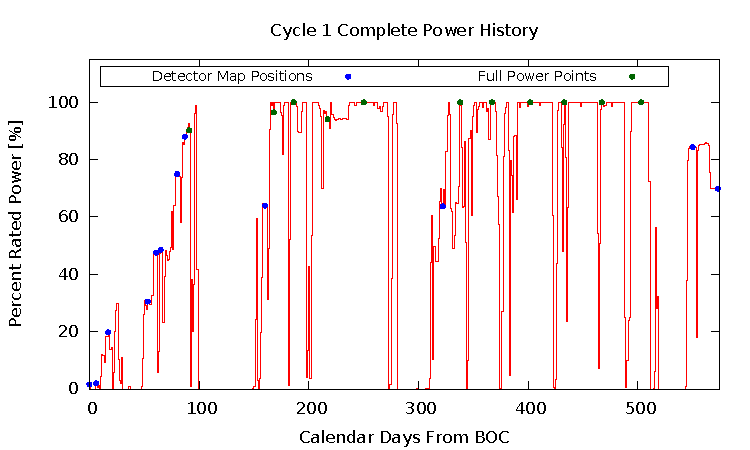
\includegraphics[width = 4.5 in]{figures/cycle1powerhist}
\caption{Cycle 1 burnup points. Full power points are indicated by green points (above 90\% power). The list of full power points (in MWd/kg) are 1.02, 1.51, 2.16, 3.30, 4.61, 6.49, 7.51, 8.70, 9.80, 11.08, 12.34.}
\label{fig:cyc1powerhist}
\end{figure}

\begin{figure}[!htb]
\centering
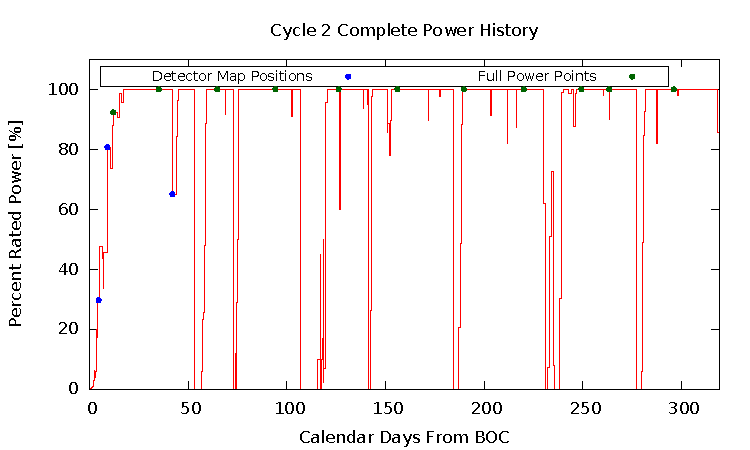
\includegraphics[width = 4.5 in]{figures/cycle2powerhist}
\caption{Cycle 2 burnup points. Full power points are indicated by green points (above 90\% power). The list of full power points (in MWd/kg) are 0.23, 1.14, 2.11, 3.20, 4.04, 5.23, 6.52, 7.71, 8.73, 9.36, 10.43.}
\label{fig:cyc2powerhist}
\end{figure}

Section \ref{sec:corewide_rms} begins by examining what core-wide RMS between Simulate and BEAVRS data looks like in order to provide a holistic perspective of how errors behave over burnup. This transitions into a narrower analysis of assembly-level behavior in Section \ref{sec:modelbias_char}, where it is found that simulations overpredict reaction rates by a small but persistent discrepancy labeled as model bias. The remaining detection uncertainty after correcting for model bias is evaluated over the entire burnup range in Section \ref{sec:cassim_timedep_uq} in an attempt to produce a core-level error heuristic over the entire cycle. Section \ref{sec:cassim_assum_valid} tests the assumptions made during this analysis, while Section \ref{sec:sim_verfiy} verifies that the results are not dependent on the model used by running the same tests with data from the MPACT model rather than the CASMO/Simulate model. Data from this model was provided by the CASL team \cite{collinsComm}. Finally, section \ref{sec:unc_combine} combines detection uncertainty with uncertainty from using tilt-corrected data to find overall time-dependent uncertainty.

\subsubsection{Visualization of Core-wide RMS}\label{sec:corewide_rms}

Time series analysis can be conducted at the core level by observing how RMS between BEAVRS and Simulate maps vary at each burnup point. This is shown in Figure \ref{fig:lm_cyc1_rms} for cycle 1 and in Figure \ref{fig:lm_cyc2_rms} for cycle 2. From these graphs it is evident that core-wide RMS essentially decreases over burnup for both cases, and that the data for cycle 2 is much smoother than for cycle 1 due to the smoother power history  in cycle 2. For cycle 1, there is reason to believe that burnup points 1.02 MWd/kg and 9.80 MWd/kg are outliers. The measurement readings at 9.80 MWd/kg happened during temporary shutdowns and sudden fluctuations, while the recordings at 1.02 MWd/kg occurred while the reactor was still ramping up and had not yet attained full power. These observations will become especially important in Section \ref{sec:cassim_assum_valid}, where it is shown that analysis conducted with the outlier burnup points in cycle 1 yields erratic results since the state of the core is not well characterized during these transition periods.

\begin{figure}[!htb]
\centering
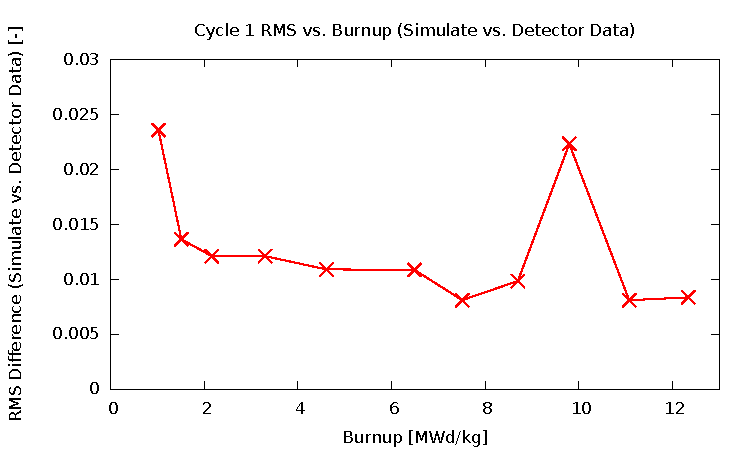
\includegraphics[keepaspectratio, width = 4.5 in]{figures/sim_rms_cyc1}
\caption{Core-wide normalized U-235 rate RMS error between CASMO-5/Simulate-3 and tilt-corrected BEAVRS data for cycle 1.}
\label{fig:lm_cyc1_rms}
\end{figure}

\begin{figure}[!htb]
\centering
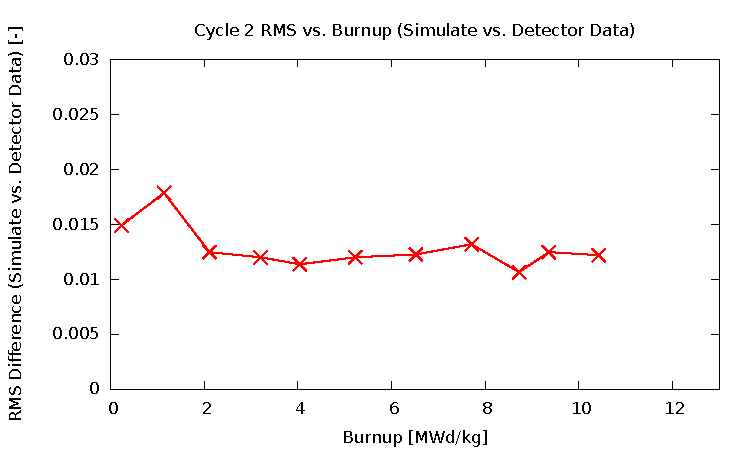
\includegraphics[keepaspectratio, width = 4.5 in]{figures/sim_rms_cyc2}
\caption{Core-wide normalized U-235 rate RMS error between CASMO-5/Simulate-3 and tilt-corrected BEAVRS data for cycle 2.}
\label{fig:lm_cyc2_rms}
\end{figure}

\subsubsection{Characterization of Model Bias}\label{sec:modelbias_char}

The focus will now shift to assembly-level CASMO/Simulate data. As aforementioned, only a subset of burnups are going to be examined at a time, due to the unstable power history. Figure \ref{fig:sim_D10_before} plots reaction rates for CASMO/Simulate and BEAVRS data for assembly D10 at the first three burnups of 1.02, 1.51, and 2.16 MWd/kg in cycle 1. Looking at this region, it is clear that the two plots exhibit a similar shape but are offset by some amount. Defining this offset as model bias, the goal is to overlay the BEAVRS data onto the CASMO/Simulate data, and then measure how much noise there is between this new data set and CASMO/Simulate. This resulting noise can be quantified as a measure of detection uncertainty. Only assemblies that have a complete data set for these three burnups are used.

\begin{figure}[!htb]
\centering
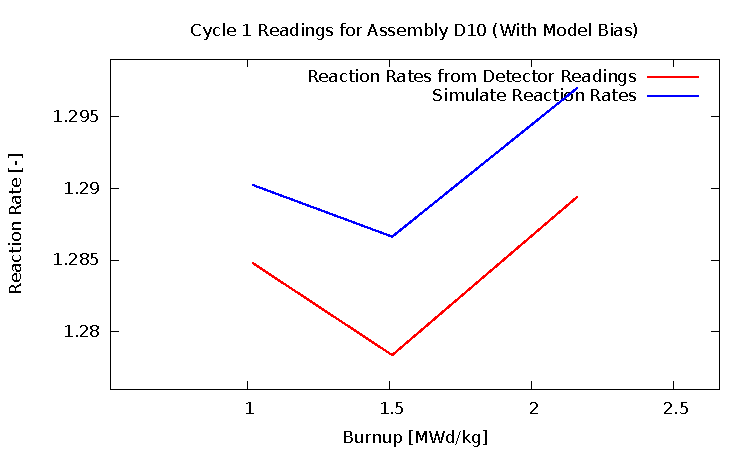
\includegraphics[keepaspectratio, width = 4.5 in]{figures/D10_before}
\caption{Reaction rates for CASMO/Simulate (blue) and BEAVRS (red) data for assembly D10 at 1.02, 1.51, and 2.16 MWd/kg.}
\label{fig:sim_D10_before}
\end{figure}

Thus, the methodology that is pursued is to calculate relative percent error at each burnup and average this value across all burnups to get an estimate of the average deviation between detector readings and simulated reaction rates. For each burnup, this average deviation is subtracted out and new detector readings are extrapolated based on this new percent error. Figure \ref{fig:sim_D10_after} shows the new extrapolated detector readings that are calculated once average relative error is subtracted out. The new BEAVRS data curve is basically a version of the original data that is overlaid onto CASMO/Simulate data. With this new curve, RMS can be quantified and deemed as detection uncertainty. Model bias in this case is defined as the RMS value of percent errors between the original BEAVRS data and CASMO/Simulate data. For assembly D10, model bias is 0.6\%, while detection uncertainty is 0.1\%.

\begin{figure}[!htb]
\centering
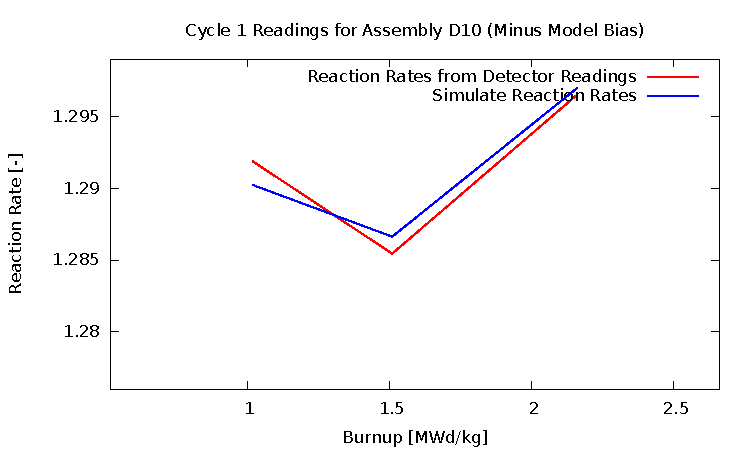
\includegraphics[keepaspectratio, width = 4.5 in]{figures/D10_after}
\caption{Reaction rates for CASMO/Simulate (blue) and BEAVRS data without model bias (red) for assembly D10 at 1.02, 1.51, and 2.16 MWd/kg.}
\label{fig:sim_D10_after}
\end{figure}

\begin{figure}[!htb]
\centering
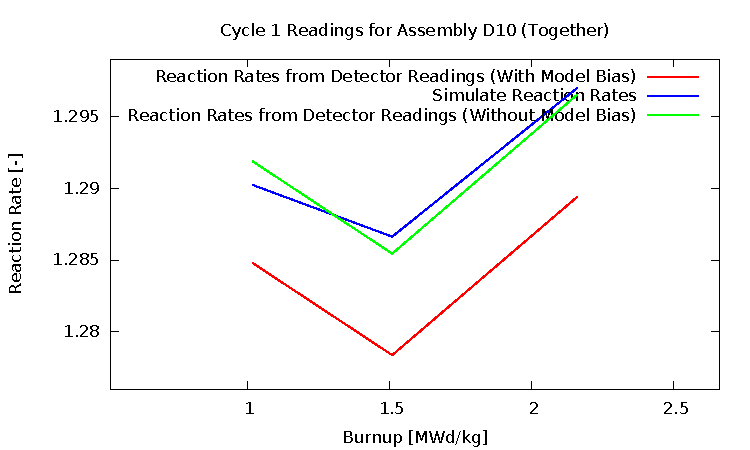
\includegraphics[keepaspectratio, width = 4.5 in]{figures/D10_together}
\caption{Reaction rates for CASMO/Simulate (blue) and BEAVRS (red) data, along with BEAVRS data with model bias subtracted out (green) for assembly D10 at 1.02, 1.51, and 2.16 MWd/kg.}
\label{fig:sim_D10_together}
\end{figure}

By extending this methodology for all assemblies within the burnup range of 1.02, 1.51, and 2.16 MWd/kg, both model bias and detection uncertainty can be quantified for all assemblies. Figure \ref{fig:sim_cyc1_eighth_map_1.02-1.51-2.16} shows the results for all assemblies within the symmetric eighth-core. Once again, an RMS value that weighs both model bias and detection uncertainty by the number of symmetric positions for that specific assembly is calculated. RMS for model bias for the entire core is 1.8\%, while the RMS for detection uncertainty is 0.9\%. 

\definecolor{Dfourteencolor}{rgb}{1,1,1}
\definecolor{Ntwocolor}{rgb}{1,1,1}
\definecolor{Gsevencolor}{rgb}{1,1,1}
\definecolor{Gsixcolor}{rgb}{1,1,1}
\definecolor{Gfivecolor}{rgb}{1,1,1}
\definecolor{Gfourcolor}{rgb}{1,1,1}
\definecolor{Gthreecolor}{rgb}{1,1,1}
\definecolor{Gtwocolor}{rgb}{1,1,1}
\definecolor{Gonecolor}{rgb}{1,1,1}
\definecolor{Nfourcolor}{rgb}{1,1,1}
\definecolor{Kfourteencolor}{rgb}{1,1,1}
\definecolor{Gninecolor}{rgb}{0.732739066549,0.8,0.16}
\definecolor{Geightcolor}{rgb}{0.659055305526,0.8,0.16}
\definecolor{Nsixcolor}{rgb}{1,1,1}
\definecolor{Nsevencolor}{rgb}{1,1,1}
\definecolor{Rfivecolor}{rgb}{1,1,1}
\definecolor{Rsixcolor}{rgb}{1,1,1}
\definecolor{Rsevencolor}{rgb}{1,1,1}
\definecolor{Reightcolor}{rgb}{1,1,1}
\definecolor{Rninecolor}{rgb}{1,1,1}
\definecolor{Jeightcolor}{rgb}{1,1,1}
\definecolor{Jninecolor}{rgb}{1,1,1}
\definecolor{Jfourcolor}{rgb}{1,1,1}
\definecolor{Jfivecolor}{rgb}{1,1,1}
\definecolor{Jsixcolor}{rgb}{1,1,1}
\definecolor{Jsevencolor}{rgb}{1,1,1}
\definecolor{Jonecolor}{rgb}{1,1,1}
\definecolor{Jtwocolor}{rgb}{1,1,1}
\definecolor{Jthreecolor}{rgb}{1,1,1}
\definecolor{Bfourcolor}{rgb}{1,1,1}
\definecolor{Bfivecolor}{rgb}{1,1,1}
\definecolor{Bsixcolor}{rgb}{1,1,1}
\definecolor{Bsevencolor}{rgb}{1,1,1}
\definecolor{Bthreecolor}{rgb}{1,1,1}
\definecolor{Ksevencolor}{rgb}{1,1,1}
\definecolor{Beightcolor}{rgb}{0.369241236076,0.8,0.16}
\definecolor{Bninecolor}{rgb}{0.222197572555,0.8,0.16}
\definecolor{Ksixcolor}{rgb}{1,1,1}
\definecolor{Nfivecolor}{rgb}{1,1,1}
\definecolor{Kfivecolor}{rgb}{1,1,1}
\definecolor{Lfourteencolor}{rgb}{1,1,1}
\definecolor{Lfifteencolor}{rgb}{1,1,1}
\definecolor{Kfourcolor}{rgb}{1,1,1}
\definecolor{Ltencolor}{rgb}{1,1,1}
\definecolor{Lelevencolor}{rgb}{1,1,1}
\definecolor{Ltwelvecolor}{rgb}{1,1,1}
\definecolor{Lthirteencolor}{rgb}{1,1,1}
\definecolor{Mfivecolor}{rgb}{1,1,1}
\definecolor{Mfourcolor}{rgb}{1,1,1}
\definecolor{Msevencolor}{rgb}{1,1,1}
\definecolor{Msixcolor}{rgb}{1,1,1}
\definecolor{Mthreecolor}{rgb}{1,1,1}
\definecolor{Mtwocolor}{rgb}{1,1,1}
\definecolor{Mninecolor}{rgb}{1,1,1}
\definecolor{Meightcolor}{rgb}{1,1,1}
\definecolor{Rtencolor}{rgb}{1,1,1}
\definecolor{Relevencolor}{rgb}{1,1,1}
\definecolor{Mfourteencolor}{rgb}{1,1,1}
\definecolor{Ptencolor}{rgb}{1,1,1}
\definecolor{Pelevencolor}{rgb}{1,1,1}
\definecolor{Ptwelvecolor}{rgb}{1,1,1}
\definecolor{Pthirteencolor}{rgb}{1,1,1}
\definecolor{Eninecolor}{rgb}{0.551397672298,0.8,0.16}
\definecolor{Eeightcolor}{rgb}{0.477342819569,0.8,0.16}
\definecolor{Efivecolor}{rgb}{1,1,1}
\definecolor{Efourcolor}{rgb}{1,1,1}
\definecolor{Esevencolor}{rgb}{1,1,1}
\definecolor{Esixcolor}{rgb}{1,1,1}
\definecolor{Eonecolor}{rgb}{1,1,1}
\definecolor{Peightcolor}{rgb}{1,1,1}
\definecolor{Ethreecolor}{rgb}{1,1,1}
\definecolor{Etwocolor}{rgb}{1,1,1}
\definecolor{Pthreecolor}{rgb}{1,1,1}
\definecolor{Pninecolor}{rgb}{1,1,1}
\definecolor{Psixcolor}{rgb}{1,1,1}
\definecolor{Psevencolor}{rgb}{1,1,1}
\definecolor{Pfourcolor}{rgb}{1,1,1}
\definecolor{Pfivecolor}{rgb}{1,1,1}
\definecolor{Htencolor}{rgb}{1,1,1}
\definecolor{Helevencolor}{rgb}{1,1,1}
\definecolor{Htwelvecolor}{rgb}{1,1,1}
\definecolor{Hthirteencolor}{rgb}{1,1,1}
\definecolor{Hfourteencolor}{rgb}{1,1,1}
\definecolor{Hfifteencolor}{rgb}{1,1,1}
\definecolor{Ftwelvecolor}{rgb}{1,1,1}
\definecolor{Fthirteencolor}{rgb}{1,1,1}
\definecolor{Ftencolor}{rgb}{0.456852857372,0.8,0.16}
\definecolor{Felevencolor}{rgb}{1,1,1}
\definecolor{Ffourteencolor}{rgb}{1,1,1}
\definecolor{Ffifteencolor}{rgb}{1,1,1}
\definecolor{Ntwelvecolor}{rgb}{1,1,1}
\definecolor{Nthirteencolor}{rgb}{1,1,1}
\definecolor{Heightcolor}{rgb}{1,1,1}
\definecolor{Nelevencolor}{rgb}{1,1,1}
\definecolor{Nfourteencolor}{rgb}{1,1,1}
\definecolor{Htwocolor}{rgb}{1,1,1}
\definecolor{Hthreecolor}{rgb}{1,1,1}
\definecolor{Honecolor}{rgb}{1,1,1}
\definecolor{Hsixcolor}{rgb}{1,1,1}
\definecolor{Hsevencolor}{rgb}{1,1,1}
\definecolor{Hfourcolor}{rgb}{1,1,1}
\definecolor{Hfivecolor}{rgb}{1,1,1}
\definecolor{Kthirteencolor}{rgb}{1,1,1}
\definecolor{Ktwelvecolor}{rgb}{1,1,1}
\definecolor{Kelevencolor}{rgb}{1,1,1}
\definecolor{Ktencolor}{rgb}{1,1,1}
\definecolor{Dtencolor}{rgb}{0.251436414306,0.8,0.16}
\definecolor{Delevencolor}{rgb}{1,1,1}
\definecolor{Dtwelvecolor}{rgb}{0.478648403082,0.8,0.16}
\definecolor{Dthirteencolor}{rgb}{1,1,1}
\definecolor{Kthreecolor}{rgb}{1,1,1}
\definecolor{Ktwocolor}{rgb}{1,1,1}
\definecolor{Konecolor}{rgb}{1,1,1}
\definecolor{Btwelvecolor}{rgb}{0.8,0.42718782238,0.16}
\definecolor{Bthirteencolor}{rgb}{0.8,0.16,0.16}
\definecolor{Btencolor}{rgb}{0.508825892302,0.8,0.16}
\definecolor{Belevencolor}{rgb}{1,1,1}
\definecolor{Kninecolor}{rgb}{1,1,1}
\definecolor{Keightcolor}{rgb}{1,1,1}
\definecolor{Nthreecolor}{rgb}{1,1,1}
\definecolor{Cninecolor}{rgb}{1,1,1}
\definecolor{Ceightcolor}{rgb}{0.186069637083,0.8,0.16}
\definecolor{Cthreecolor}{rgb}{1,1,1}
\definecolor{Ctwocolor}{rgb}{1,1,1}
\definecolor{Kfifteencolor}{rgb}{1,1,1}
\definecolor{Jfifteencolor}{rgb}{1,1,1}
\definecolor{Csevencolor}{rgb}{1,1,1}
\definecolor{Csixcolor}{rgb}{1,1,1}
\definecolor{Cfivecolor}{rgb}{1,1,1}
\definecolor{Cfourcolor}{rgb}{1,1,1}
\definecolor{Etwelvecolor}{rgb}{1,1,1}
\definecolor{Ntencolor}{rgb}{1,1,1}
\definecolor{Neightcolor}{rgb}{1,1,1}
\definecolor{Nninecolor}{rgb}{1,1,1}
\definecolor{Hninecolor}{rgb}{1,1,1}
\definecolor{Gfifteencolor}{rgb}{1,1,1}
\definecolor{Gfourteencolor}{rgb}{1,1,1}
\definecolor{Gthirteencolor}{rgb}{1,1,1}
\definecolor{Gtwelvecolor}{rgb}{1,1,1}
\definecolor{Gelevencolor}{rgb}{1,1,1}
\definecolor{Gtencolor}{rgb}{1,1,1}
\definecolor{Fonecolor}{rgb}{1,1,1}
\definecolor{Ftwocolor}{rgb}{1,1,1}
\definecolor{Fthreecolor}{rgb}{1,1,1}
\definecolor{Ffourcolor}{rgb}{1,1,1}
\definecolor{Ffivecolor}{rgb}{1,1,1}
\definecolor{Fsixcolor}{rgb}{1,1,1}
\definecolor{Fsevencolor}{rgb}{1,1,1}
\definecolor{Feightcolor}{rgb}{0.198337851388,0.8,0.16}
\definecolor{Fninecolor}{rgb}{0.587010931801,0.8,0.16}
\definecolor{Jthirteencolor}{rgb}{1,1,1}
\definecolor{Melevencolor}{rgb}{1,1,1}
\definecolor{Mtencolor}{rgb}{1,1,1}
\definecolor{Mthirteencolor}{rgb}{1,1,1}
\definecolor{Mtwelvecolor}{rgb}{1,1,1}
\definecolor{Jtencolor}{rgb}{1,1,1}
\definecolor{Jelevencolor}{rgb}{1,1,1}
\definecolor{Eelevencolor}{rgb}{0.297746908296,0.8,0.16}
\definecolor{Etencolor}{rgb}{0.473790355304,0.8,0.16}
\definecolor{Ethirteencolor}{rgb}{1,1,1}
\definecolor{Jfourteencolor}{rgb}{1,1,1}
\definecolor{Efifteencolor}{rgb}{1,1,1}
\definecolor{Efourteencolor}{rgb}{1,1,1}
\definecolor{Cthirteencolor}{rgb}{0.8,0.548828881999,0.16}
\definecolor{Ctwelvecolor}{rgb}{0.575930791061,0.8,0.16}
\definecolor{Celevencolor}{rgb}{0.417154048511,0.8,0.16}
\definecolor{Ctencolor}{rgb}{0.176911660885,0.8,0.16}
\definecolor{Cfourteencolor}{rgb}{1,1,1}
\definecolor{Aelevencolor}{rgb}{0.8,0.6376035379,0.16}
\definecolor{Atencolor}{rgb}{0.334891704259,0.8,0.16}
\definecolor{Afivecolor}{rgb}{1,1,1}
\definecolor{Asevencolor}{rgb}{1,1,1}
\definecolor{Asixcolor}{rgb}{1,1,1}
\definecolor{Aninecolor}{rgb}{0.16,0.8,0.16}
\definecolor{Aeightcolor}{rgb}{0.178315965399,0.8,0.16}
\definecolor{Jtwelvecolor}{rgb}{1,1,1}
\definecolor{Lsixcolor}{rgb}{1,1,1}
\definecolor{Lsevencolor}{rgb}{1,1,1}
\definecolor{Lfourcolor}{rgb}{1,1,1}
\definecolor{Lfivecolor}{rgb}{1,1,1}
\definecolor{Ltwocolor}{rgb}{1,1,1}
\definecolor{Lthreecolor}{rgb}{1,1,1}
\definecolor{Lonecolor}{rgb}{1,1,1}
\definecolor{Leightcolor}{rgb}{1,1,1}
\definecolor{Lninecolor}{rgb}{1,1,1}
\definecolor{Deightcolor}{rgb}{0.248726735829,0.8,0.16}
\definecolor{Dninecolor}{rgb}{0.268380693734,0.8,0.16}
\definecolor{Dsixcolor}{rgb}{1,1,1}
\definecolor{Dsevencolor}{rgb}{1,1,1}
\definecolor{Dfourcolor}{rgb}{1,1,1}
\definecolor{Dfivecolor}{rgb}{1,1,1}
\definecolor{Dtwocolor}{rgb}{1,1,1}
\definecolor{Dthreecolor}{rgb}{1,1,1}

\begin{figure}[!htb]
    \centering
    
    % these dimensions are determined in arrow_dimms.ods
    
    \def\scale{2.0}

    \def\latWidth{0.2673473684*\scale}
    
    \def\RPVOR{3*\scale}
    \def\rectW{0.75*\scale}
    \def\RPVIR{2.7315789474*\scale}
    \def\BarrelIR{2.3368421053*\scale}
    \def\BarrelOR{2.4078947368*\scale}
    \def\ShieldIR{2.4223787816*\scale}
    \def\ShieldOR{2.5067965189*\scale}
    \def\LinerIR{2.7246166598*\scale}

    \def\bafCIRx{0.9357157895*\scale}
    \def\bafCIRy{2.0051052632*\scale}
    \def\bafCORx{0.9633473684*\scale}
    \def\bafCORy{2.0327368421*\scale}
    \def\bafMIRx{1.7377578947*\scale}
    \def\bafMIRy{1.4704105263*\scale}
    \def\bafMORx{1.7653894737*\scale}
    \def\bafMORy{1.4980421053*\scale}
    
    \tikzset{Assembly/.style={
        inner sep=0pt,
        text width=\latWidth in,
        minimum size=\latWidth in,
        draw=black,
        align=center
        }
    }
    
    \def\tkzRPV{(0,0) circle (\RPVIR) (0,0) circle (\RPVOR)}
    \def\tkzLiner{(0,0) circle (\LinerIR) (0,0) circle (\RPVIR)}
    \def\tkzBarrel{(0,0) circle (\BarrelIR) (0,0) circle (\BarrelOR)}
    \def\tkzShields{(0,0) circle (\ShieldIR) (0,0) circle (\ShieldOR)}
    
    \def\tkzBaffCOR{(-\bafCORx, -\bafCORy) rectangle (\bafCORx, \bafCORy)}
    \def\tkzBaffCIR{(-\bafCIRx, -\bafCIRy) rectangle (\bafCIRx, \bafCIRy)} 
    \def\tkzBaffMOR{(-\bafMORx, -\bafMORy) rectangle (\bafMORx, \bafMORy)}
    \def\tkzBaffMIR{(-\bafMIRx, -\bafMIRy) rectangle (\bafMIRx, \bafMIRy) }
    \def\tkzBaffleC{ \tkzBaffCIR \tkzBaffCOR }
    \def\tkzBaffleM{ \tkzBaffMIR \tkzBaffMOR }

    \def\tkzBaffCClip{\tkzBaffCIR (-\RPVOR, -\RPVOR) rectangle (\RPVOR, \RPVOR)}
    \def\tkzBaffMClip{\tkzBaffMIR (-\RPVOR, -\RPVOR) rectangle (\RPVOR, \RPVOR)}

    \def\highenr{blue!50}
    \def\midenr{yellow!50}
    \def\lowenr{red!50}
    
    \scalebox{0.6}{
    
      \begin{tikzpicture}[x=1in,y=1in]
      \fontfamily{mdbch}\selectfont
      
        %\begin{scope}
          %\clip ($(-\latWidth/2,\latWidth/2)$) rectangle (\RPVOR,-\RPVOR);
          % draw RPV, barrel, and shield panels
          
          %\path[fill=black!90!white,even odd rule] \tkzRPV;
          %\path[fill=black,even odd rule] \tkzLiner;
          %\path[fill=black,even odd rule] \tkzBarrel;
          %\begin{scope}
          %  \clip (0,0) -- +(61:\RPVOR) arc (61:29:\RPVOR) --
          %        (0,0) -- +(151:\RPVOR) arc (151:119:\RPVOR) -- 
          %        (0,0) -- +(241:\RPVOR) arc (241:209:\RPVOR) -- 
          %        (0,0) -- +(331:\RPVOR) arc (331:299:\RPVOR) -- cycle;
          %  \path[fill=black,even odd rule] \tkzShields;
          %\end{scope}

          % draw baffle north/south
          
          %\begin{scope}[even odd rule]
          %  \clip[rotate=90] \tkzBaffMClip;
          %  \path[fill=black] \tkzBaffleC;
          %\end{scope}
          %\begin{scope}[even odd rule]
          %  \clip \tkzBaffCClip;
          %  \clip \tkzBaffMClip;
          %  \path[fill=black, rotate=90] \tkzBaffleM;
          %\end{scope}
          
          % draw baffle east/west
          
          %\begin{scope}[rotate=90]
          %  \begin{scope}[even odd rule]
          %    \clip[rotate=90] \tkzBaffMClip;
          %    \path[fill=black] \tkzBaffleC;
          %  \end{scope}
          %  \begin{scope}[even odd rule]
          %    \clip \tkzBaffCClip;
          %    \clip \tkzBaffMClip;
          %    \path[fill=black, rotate=90] \tkzBaffleM;
          %  \end{scope}
          %\end{scope}
          
        %\end{scope}
        
        % draw assembly row/column headers
        
        \draw[red, thick] ($(-0*\latWidth,1*\latWidth)$) node[above, anchor=south] {H} -- ($(-0*\latWidth,0.6*\latWidth)$);
        \draw[red, thick] ($(1*\latWidth,1*\latWidth)$) node[above, anchor=south] {G} -- ($(1*\latWidth,0.6*\latWidth)$);
        \draw[red, thick] ($(2*\latWidth,1*\latWidth)$) node[above, anchor=south] {F} -- ($(2*\latWidth,0.6*\latWidth)$);
        \draw[red, thick] ($(3*\latWidth,1*\latWidth)$) node[above, anchor=south] {E} -- ($(3*\latWidth,0.6*\latWidth)$);
        \draw[red, thick] ($(4*\latWidth,1*\latWidth)$) node[above, anchor=south] {D} -- ($(4*\latWidth,0.6*\latWidth)$);
        \draw[red, thick] ($(5*\latWidth,1*\latWidth)$) node[above, anchor=south] {C} -- ($(5*\latWidth,0.6*\latWidth)$);
        \draw[red, thick] ($(6*\latWidth,1*\latWidth)$) node[above, anchor=south] {B} -- ($(6*\latWidth,0.6*\latWidth)$);
        \draw[red, thick] ($(7*\latWidth,1*\latWidth)$) node[above, anchor=south] {A} -- ($(7*\latWidth,0.6*\latWidth)$);
        
        \begin{scope}[rotate=90]
          \draw[red, thick] ($(-7*\latWidth,1*\latWidth)$) node[left, anchor=east] {15} -- ($(-7*\latWidth,0.6*\latWidth)$);
          \draw[red, thick] ($(-6*\latWidth,1*\latWidth)$) node[left, anchor=east] {14} -- ($(-6*\latWidth,0.6*\latWidth)$);
          \draw[red, thick] ($(-5*\latWidth,1*\latWidth)$) node[left, anchor=east] {13} -- ($(-5*\latWidth,0.6*\latWidth)$);
          \draw[red, thick] ($(-4*\latWidth,1*\latWidth)$) node[left, anchor=east] {12} -- ($(-4*\latWidth,0.6*\latWidth)$);
          \draw[red, thick] ($(-3*\latWidth,1*\latWidth)$) node[left, anchor=east] {11} -- ($(-3*\latWidth,0.6*\latWidth)$);
          \draw[red, thick] ($(-2*\latWidth,1*\latWidth)$) node[left, anchor=east] {10} -- ($(-2*\latWidth,0.6*\latWidth)$);
          \draw[red, thick] ($(-1*\latWidth,1*\latWidth)$) node[left, anchor=east] {9} -- ($(-1*\latWidth,0.6*\latWidth)$);
          \draw[red, thick] ($(-0*\latWidth,1*\latWidth)$) node[left, anchor=east] {8} -- ($(-0*\latWidth,0.6*\latWidth)$);
        \end{scope}
        
        % draw fuel assembly nodes

        \node [Assembly, fill=Heightcolor] at ($(-0*\latWidth,0*\latWidth)$) {}; % H8
        \node [Assembly, fill=Geightcolor] at ($( 1*\latWidth,0*\latWidth)$) {

\scriptsize{0.019} 
 \scriptsize{0.002} 

}; % G8
        \node [Assembly, fill=Feightcolor] at ($( 2*\latWidth,0*\latWidth)$) {

\scriptsize{0.004} 
 \scriptsize{0.003} 

}; % F8
        \node [Assembly, fill=Eeightcolor] at ($( 3*\latWidth,0*\latWidth)$) {

\scriptsize{0.013} 
 \scriptsize{0.009} 

}; % E8
        \node [Assembly, fill=Deightcolor] at ($( 4*\latWidth,0*\latWidth)$) {

\scriptsize{0.005} 
 \scriptsize{0.003} 

}; % D8
        \node [Assembly, fill=Ceightcolor] at ($( 5*\latWidth,0*\latWidth)$) {

\scriptsize{0.003} 
 \scriptsize{0.001} 

}; % C8
        \node [Assembly, fill=Beightcolor] at ($( 6*\latWidth,0*\latWidth)$) {

\scriptsize{0.009} 
 \scriptsize{0.006} 

}; % B8
        \node [Assembly, fill=Aeightcolor] at ($( 7*\latWidth,0*\latWidth)$) {

\scriptsize{0.003} 
 \scriptsize{0.003} 

}; % A8

        \node [Assembly, fill=Hninecolor] at ($(-0*\latWidth,-1*\latWidth)$) {}; % H9
        \node [Assembly, fill=Gninecolor] at ($( 1*\latWidth,-1*\latWidth)$) {

\scriptsize{0.021} 
 \scriptsize{0.016} 

}; % G9
        \node [Assembly, fill=Fninecolor] at ($( 2*\latWidth,-1*\latWidth)$) {

\scriptsize{0.017} 
 \scriptsize{0.002} 

}; % F9
        \node [Assembly, fill=Eninecolor] at ($( 3*\latWidth,-1*\latWidth)$) {

\scriptsize{0.015} 
 \scriptsize{0.012} 

}; % E9
        \node [Assembly, fill=Dninecolor] at ($( 4*\latWidth,-1*\latWidth)$) {

\scriptsize{0.006} 
 \scriptsize{0.003} 

}; % D9
        \node [Assembly, fill=Cninecolor] at ($( 5*\latWidth,-1*\latWidth)$) {}; % C9
        \node [Assembly, fill=Bninecolor] at ($( 6*\latWidth,-1*\latWidth)$) {

\scriptsize{0.005} 
 \scriptsize{0.004} 

}; % B9
        \node [Assembly, fill=Aninecolor] at ($( 7*\latWidth,-1*\latWidth)$) {

\scriptsize{0.003} 
 \scriptsize{0.003} 

}; % A9

        \node [Assembly, fill=Htencolor] at ($(-0*\latWidth,-2*\latWidth)$) {}; % H10
        \node [Assembly, fill=Gtencolor] at ($( 1*\latWidth,-2*\latWidth)$) {}; % G10
        \node [Assembly, fill=Ftencolor] at ($( 2*\latWidth,-2*\latWidth)$) {

\scriptsize{0.012} 
 \scriptsize{0.010} 

}; % F10
        \node [Assembly, fill=Etencolor] at ($( 3*\latWidth,-2*\latWidth)$) {

\scriptsize{0.013} 
 \scriptsize{0.003} 

}; % E10
        \node [Assembly, fill=Dtencolor] at ($( 4*\latWidth,-2*\latWidth)$) {

\scriptsize{0.006} 
 \scriptsize{0.001} 

}; % D10
        \node [Assembly, fill=Ctencolor] at ($( 5*\latWidth,-2*\latWidth)$) {

\scriptsize{0.003} 
 \scriptsize{0.003} 

}; % C10
        \node [Assembly, fill=Btencolor] at ($( 6*\latWidth,-2*\latWidth)$) {

\scriptsize{0.014} 
 \scriptsize{0.002} 

}; % B10
        \node [Assembly, fill=Atencolor] at ($( 7*\latWidth,-2*\latWidth)$) {

\scriptsize{0.008} 
 \scriptsize{0.008} 

}; % A10

        \node [Assembly, fill=Helevencolor] at ($(-0*\latWidth,-3*\latWidth)$) {}; % H11
        \node [Assembly, fill=Gelevencolor] at ($( 1*\latWidth,-3*\latWidth)$) {}; % G11
        \node [Assembly, fill=Felevencolor] at ($( 2*\latWidth,-3*\latWidth)$) {}; % F11
        \node [Assembly, fill=Eelevencolor] at ($( 3*\latWidth,-3*\latWidth)$) {

\scriptsize{0.007} 
 \scriptsize{0.007} 

}; % E11
        \node [Assembly, fill=Delevencolor] at ($( 4*\latWidth,-3*\latWidth)$) {}; % D11
        \node [Assembly, fill=Celevencolor] at ($( 5*\latWidth,-3*\latWidth)$) {

\scriptsize{0.011} 
 \scriptsize{0.011} 

}; % C11
        \node [Assembly, fill=Belevencolor] at ($( 6*\latWidth,-3*\latWidth)$) {}; % B11
        \node [Assembly, fill=Aelevencolor] at ($( 7*\latWidth,-3*\latWidth)$) {

\scriptsize{0.029} 
 \scriptsize{0.015} 

}; % A11

        \node [Assembly, fill=Htwelvecolor] at ($(-0*\latWidth,-4*\latWidth)$) {}; % H12
        \node [Assembly, fill=Gtwelvecolor] at ($( 1*\latWidth,-4*\latWidth)$) {}; % G12
        \node [Assembly, fill=Ftwelvecolor] at ($( 2*\latWidth,-4*\latWidth)$) {}; % F12
        \node [Assembly, fill=Etwelvecolor] at ($( 3*\latWidth,-4*\latWidth)$) {}; % E12
        \node [Assembly, fill=Dtwelvecolor] at ($( 4*\latWidth,-4*\latWidth)$) {

\scriptsize{0.013} 
 \scriptsize{0.012} 

}; % D12
        \node [Assembly, fill=Ctwelvecolor] at ($( 5*\latWidth,-4*\latWidth)$) {

\scriptsize{0.016} 
 \scriptsize{0.012} 

}; % C12
        \node [Assembly, fill=Btwelvecolor] at ($( 6*\latWidth,-4*\latWidth)$) {

\scriptsize{0.036} 
 \scriptsize{0.020} 

}; % B12

        \node [Assembly, fill=Hthirteencolor] at ($(-0*\latWidth,-5*\latWidth)$) {}; % H13
        \node [Assembly, fill=Gthirteencolor] at ($( 1*\latWidth,-5*\latWidth)$) {}; % G13
        \node [Assembly, fill=Fthirteencolor] at ($( 2*\latWidth,-5*\latWidth)$) {}; % F13
        \node [Assembly, fill=Ethirteencolor] at ($( 3*\latWidth,-5*\latWidth)$) {}; % E13
        \node [Assembly, fill=Dthirteencolor] at ($( 4*\latWidth,-5*\latWidth)$) {}; % D13
        \node [Assembly, fill=Cthirteencolor] at ($( 5*\latWidth,-5*\latWidth)$) {

\scriptsize{0.032} 
 \scriptsize{0.006} 

}; % C13
        \node [Assembly, fill=Bthirteencolor] at ($( 6*\latWidth,-5*\latWidth)$) {

\scriptsize{0.045} 
 \scriptsize{0.010} 

}; % B13

        \node [Assembly, fill=Hfourteencolor] at ($(-0*\latWidth,-6*\latWidth)$) {}; % H14
        \node [Assembly, fill=Gfourteencolor] at ($( 1*\latWidth,-6*\latWidth)$) {}; % G14
        \node [Assembly, fill=Ffourteencolor] at ($( 2*\latWidth,-6*\latWidth)$) {}; % F14
        \node [Assembly, fill=Efourteencolor] at ($( 3*\latWidth,-6*\latWidth)$) {}; % E14
        \node [Assembly, fill=Dfourteencolor] at ($( 4*\latWidth,-6*\latWidth)$) {}; % D14
        \node [Assembly, fill=Cfourteencolor] at ($( 5*\latWidth,-6*\latWidth)$) {}; % C14

        \node [Assembly, fill=Hfifteencolor] at ($(-0*\latWidth,-7*\latWidth)$) {}; % H15
        \node [Assembly, fill=Gfifteencolor] at ($( 1*\latWidth,-7*\latWidth)$) {}; % G15
        \node [Assembly, fill=Ffifteencolor] at ($( 2*\latWidth,-7*\latWidth)$) {}; % F15
        \node [Assembly, fill=Efifteencolor] at ($( 3*\latWidth,-7*\latWidth)$) {}; % E15
        
      \end{tikzpicture}
    }
    


    \caption{Cycle 1 model bias (top) and detection uncertainty (bottom) based on CASMO/Simulate model. Burnups: (1.02 1.51 2.16). Assembly-weighted model bias: 0.018. Assembly-weighted detection uncertainty: 0.009. \label{fig:sim_cyc1_eighth_map_1.02-1.51-2.16}}
\end{figure}



\subsubsection{Quantifying Detection Uncertainty Over Entire Burnup Range}\label{sec:cassim_timedep_uq}

Assuming that burnup sets with non-overlapping points are independent of each other, Simulate data is now fitted for the remaining 8 burnup points that were not included in the first burnup set (1.02, 1.51, 2.16). The remaining 8 points are divided into two sets of four burnups so that Simulate data is compared to the burnup sets (3.3 4.61 6.49 7.51) and (8.7 9.8 11.08 12.34). The results for assembly-weighted core-wide model bias and detection uncertainty are summarized for all burnup ranges in Table \ref{table:cyc_mb_tu}. For cycle 2, the entire burnup range is divided up in a similar manner, where core model bias and detection uncertainties are computed for the burnup sets (0.23, 1.14, 2.11), (3.20, 4.04, 5.23, 6.52), and (7.71, 8.73, 9.36, 10.43). The results for cycle 2 are also given in Table \ref{table:cyc_mb_tu}.

\begin{table}[!htb]
  \centering
  \begin{tabular}{CCC}\toprule
     Cycle 1 Burnup Points & Core-Wide \newline Model Bias (RMS) & Core-Wide Detection Uncertainty (RMS) \\ \midrule
     (1.02, 1.51, 2.16) & 1.8\% & 0.9\% \\
     (3.30, 4.61, 6.49, 7.51) & 1.1\% & 0.6\% \\
     (8.70, 9.80, 11.08, 12.34) & 1.4\% & 0.9\% \\
     \toprule
     Cycle 2 Burnup Points & Core-Wide \newline Model Bias (RMS) & Core-Wide Detection Uncertainty (RMS) \\ \midrule
     (0.23, 1.14, 2.11) & 1.6\% & 0.6\% \\
     (3.20, 4.04, 5.23, 6.52) & 1.2\% & 0.3\% \\
     (7.71, 8.73, 9.36, 10.43) & 1.2\% & 0.5\% \\ \bottomrule
  \end{tabular}
  \caption{Assembly-weighted model bias and detection uncertainty for all burnup sets in cycles 1 and 2.}
  \label{table:cyc_mb_tu}
\end{table}

Subdivision of the entire burnup range is carried out in such a way in order to extract detector variations from CASMO/Simulate data over a suitable time interval. Section \ref{sec:cassim_assum_valid} will look at the validity of burnup sets with non-overlapping points being independent of each other as well as how credible results are of being independent of burnup subdivision.

Now that BEAVRS data has been overlaid onto SIMULATE data to remove model bias, all remaining relative errors between BEAVRS data and SIMULATE data for each assembly over the three burnup divisions can be aggregated as a histogram to find a 95\% confidence level uncertainty.  Figure \ref{fig:sim_cyc1_hist_wo_mb} plots errors between BEAVRS data and SIMULATE data for cycle 1, where the histogram frequencies are weighted by the number of symmetric assembly positions. 

\begin{figure}[!htb]
\centering
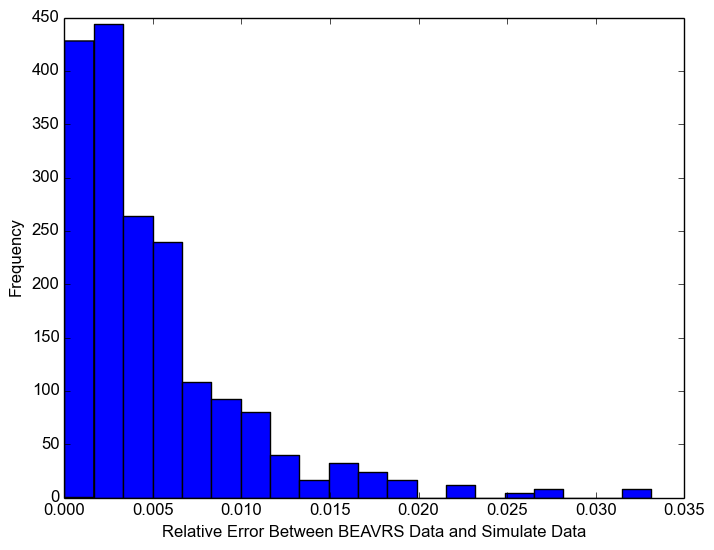
\includegraphics[keepaspectratio, height = 3.5 in]{figures/sim_cyc1_hist_wo_mb}
\caption{Histogram of relative error between Simulate Data and BEAVRS data after correcting for model bias within all assemblies over all burnups in cycle 1. RMS = 0.8\%, 95\% level = 1.6\%.}
\label{fig:sim_cyc1_hist_wo_mb}
\end{figure}

From this histogram, it is clear that errors are skewed towards the lower end, with a few large outliers on the higher end. The RMS value for detection uncertainty in cycle 1 is 0.8\%, but taking a more conservative error estimate of 95\% confidence yields a much higher detection uncertainty of 1.6\% for cycle 1. Following a similar procedure for cycle 2 yields a 95\% confidence value of 0.9\% for detection uncertainty. 

\subsubsection{Validation of Assumptions for the CASMO/Simulate Model}\label{sec:cassim_assum_valid}

There are two main assumptions that were made when calculating the results by using the CASMO/Simulate model. Firstly, the entire burnup range for both cycles were subdivided into three non-overlapping burnup ranges containing three or four burnups, and it needs to be shown that the results are not dependent on how the subdivisions were made. More specifically, for cycle 1, the entire burnup set (in MWd/kg) is subdivided into the three burnup ranges of (1.02, 1.51, 2.16), (3.30, 4.04, 5.23, 6.52), and (7.61, 8.73, 9.36, 10.43). However, the subdivision could have also been (1.02, 1.51, 2.16, 3.30), (4.04, 5.23, 6.52), and (7.61, 8.73, 9.36, 10.43). Thus, it needs to be shown that detection uncertainty results are independent of the burnup subdivision choice. Table \ref{table:bu_subdiv_sensitivity} shows the results for the 95\% confidence interval (CI) of detection uncertainty for all possible burnup subdivisions for both cycle 1 and cycle 2, and the results show that there is very little change in the results.

\begin{table}[!htb]
  \centering
  \begin{tabular}{DDDD}\toprule
     \multicolumn{3}{c}{Cycle 1 Burnup Subdivision} & 95\% CI of Detection Uncertainty \\ \midrule
     \multicolumn{3}{l}{(1.02 1.51 2.16) - (3.30 4.61 6.49 7.51) - (8.70 9.80 11.08 12.34)} & 1.6\% \\
     \multicolumn{3}{l}{(1.02 1.51 2.16 3.30) - (4.61 6.49 7.51) - (8.70 9.80 11.08 12.34)} & 1.7\% \\
     \multicolumn{3}{l}{(1.02 1.51 2.16 3.30) - (4.61 6.49 7.51 8.70) - (9.80 11.08 12.34)} & 1.6\% \\
     \toprule
     \multicolumn{3}{c}{Cycle 2 Burnup Subdivision} & 95\% CI of Detection Uncertainty \\ \midrule
     \multicolumn{3}{l}{(0.23 1.14 2.11) - (3.20 4.04 5.23 6.52) - (7.71 8.73 9.36 10.43)} & 0.9\% \\
     \multicolumn{3}{l}{(0.23 1.14 2.11 3.20) - (4.04 5.23 6.52) - (7.71 8.73 9.36 10.43)} & 1.0\% \\
     \multicolumn{3}{l}{(0.23 1.14 2.11 3.20) - (4.04 5.23 6.52 7.71) - (8.73 9.36 10.43)} & 0.9\% \\ \bottomrule
  \end{tabular}
  \caption{Results of detection uncertainty based on three different ways of subdividing all burnups  for each cycle.}
  \label{table:bu_subdiv_sensitivity}
\end{table}

The second assumption that needs to be validated that requires a bit more work is to show that non-overlapping burnup subdivisions within the entire burnup set are actually independent of each other. For example, if cycle 1 burnups are divided into the three ranges, (1.02, 1.51, 2.16), (3.30, 4.04, 5.23, 6.52), and (7.61, 8.73, 9.36, 10.43) as before, it needs to be shown that the three burnup ranges are independent of each other. To do this, the results of assembly-weighted detection uncertainty for all adjacent burnup choices of length 3 or 4 are looked at after accounting for model bias. If all non-overlapping burnup ranges of length 3 or 4 are truly independent of each other, then the results for detection uncertainty should remain the same regardless of how these burnups are chosen, so long as those burnups are adjacent to each other and represent a short interval for which predictive models are considered accurate. Table \ref{table:bu_index_len3} summarizes the results for detection uncertainty for all possible adjacent burnup choices of length 3 in cycle 1 and 2, while Table \ref{table:bu_index_len4} summarizes the results for burnup choices of length 4 in cycle 1 and 2.

\begin{table}[!htb]
  \centering
  \begin{tabular}{DDDD}\toprule
     Cycle 1 Burnup Choice & Detection Uncertainty (RMS) & Cycle 2 Burnup Choice & Detection Uncertainty (RMS) \\ \midrule
     \textcolor{red}{1.02} 1.51 2.16 & \textcolor{red}{0.9\%} & 0.23 1.14 2.11 & 0.6\% \\
     1.51 2.16 3.30 & 0.3\% & 1.14 2.11 3.2 & 0.5\% \\
     2.16 3.30 4.61 & 0.3\% & 2.11 3.2 4.04 & 0.4\% \\
     3.30 4.61 6.49 & 0.5\% & 3.2 4.04 5.23 & 0.3\% \\
     4.61 6.49 7.51 & 0.5\% & 4.04 5.23 6.52 & 0.3\% \\
     6.49 7.51 8.70 & 0.4\% & 5.23 6.52 7.71 & 0.5\% \\
     7.51 8.70 \textcolor{red}{9.80} & \textcolor{red}{1.0\%} & 6.52 7.71 8.73 & 0.5\% \\
     8.70 \textcolor{red}{9.80} 11.08 & \textcolor{red}{0.9\%} & 7.71 8.73 9.36 & 0.5\% \\
     \textcolor{red}{9.80} 11.08 12.34 & \textcolor{red}{0.8\%} & 8.73 9.36 10.43 & 0.3\% \\ \bottomrule
  \end{tabular}
  \caption{RMS of detection uncertainty when looking at all combinations of burnup subsets of length 3 in cycle 1 and cycle 2. Outliers are marked in red.}
  \label{table:bu_index_len3}
\end{table}

%COM (define all column types)

\begin{table}[!htb]
  \centering
  \begin{tabular}{FDED}\toprule
     Cycle 1 Burnup Choice & Detection Uncertainty (RMS) & Cycle 2 Burnup Choice & Detection Uncertainty (RMS) \\ \midrule
     \textcolor{red}{1.02} 1.51 2.16 3.30 & \textcolor{red}{0.8\%} & 0.23 1.14 2.11 3.20 & 0.6\% \\
     1.51 2.16 3.30 4.61 & 0.4\% & 1.14 2.11 3.20 4.04 & 0.6\% \\
     2.16 3.30 4.61 6.49 & 0.5\% & 2.11 3.20 4.04 5.23 & 0.4\% \\
     3.30 4.61 6.49 7.51 & 0.5\% & 3.20 4.04 5.23 6.52 & 0.3\% \\
     4.61 6.49 7.51 8.70 & 0.5\% & 4.04 5.23 6.52 7.71 & 0.5\% \\
     6.49 7.51 8.70 \textcolor{red}{9.80} & \textcolor{red}{1.0\%} & 5.23 6.52 7.71 8.73 & 0.5\% \\
     7.51 8.70 \textcolor{red}{9.80} 11.08 & \textcolor{red}{1.0\%} & 6.52 7.71 8.73 9.36 & 0.5\% \\
     8.70 \textcolor{red}{9.80} 11.08 12.34 & \textcolor{red}{0.9\%} & 7.71 8.73 9.36 10.43 & 0.5\% \\ \bottomrule
  \end{tabular}
  \caption{RMS of detection uncertainty when looking at all combinations of burnup subsets of length 4 in cycle 1 and cycle 2. Outliers are marked in red.}
  \label{table:bu_index_len4}
\end{table}


From these two tables, it can be seen that RMS values of detection uncertainty and model bias are roughly consistent for all burnups of length 3 and 4 in cycle 2, where RMS of detection uncertainty ranges from 0.3\% to 0.6\%. However, within cycle 1, there are some burnup subsets that have inflated RMS values totaling as much as 1.0\%, and these entries are marked in red. In addition, the burnup points common to these high error points are also highlighted in red, and outliers are driving up uncertainty values. With the presence of these outlier burnup points, the errors are much higher than in other cases. With the presence of these outliers, the assumption that the results of non-overlapping burnup sets are independent does not hold true.

Recall that these highlighted burnups are the same ones that were found in Section \ref{sec:corewide_rms} to have added model inaccuracies simply due to unstable operating conditions, further corroborating the existence of outliers at these two points. The simplest way to deal with these outliers is to remove them from the complete burnup range, redo the analysis, and see how the results change. Without these outliers, the detection uncertainties are lower and are also now consistent among all burnup choices for both cycles. The total remaining number of burnup points in the complete range after removing outliers in cycle 1 is now 9, so the burnup range is subdivided into 3 burnup sets of length three. There is no need for another sensitivity analysis based on how to subdivide the entire burnup range as there is now only one way of subdividing the entire burnup range into subsets of length 3.

\begin{table}[!htb]
  \centering
  \begin{tabular}{BB}\toprule
     Cycle 1 95\% CI of \newline Detection Uncertainty \newline (with outliers)  & Cycle 1 95\% CI of \newline Detection Uncertainty \newline (without outliers) \\ \midrule
     1.6\% & 0.8\% \\ \bottomrule
  \end{tabular}
  \caption{Cycle 1 95\% CI of detection uncertainty with and without outliers at 1.02 and 9.80 MWd/kg.}
  \label{table:cassim_results_updated}
\end{table}


\begin{table}[!htb]
  \centering
  \begin{tabular}{CCC}\toprule
     \multicolumn{2}{c}{Cycle 1 Burnup Choice} & Detection Uncertainty (RMS) \\ \midrule
     \multicolumn{2}{c}{1.51 2.16 3.30} & 0.3\% \\
     \multicolumn{2}{c}{2.16 3.30 4.61} & 0.3\% \\
     \multicolumn{2}{c}{3.30 4.61 6.49} & 0.5\% \\
     \multicolumn{2}{c}{4.61 6.49 7.51} & 0.5\% \\
     \multicolumn{2}{c}{6.49 7.51 8.70} & 0.4\% \\
     \multicolumn{2}{c}{7.51 8.70 11.08} & 0.4\% \\
     \multicolumn{2}{c}{8.70 11.08 12.34} & 0.4\% \\ \bottomrule
  \end{tabular}
  \caption{RMS of detection uncertainty when looking at all combinations of burnup subsets of length 3 in cycle 1 when outliers at 1.02 and 9.80 MWd/kg are removed.}
  \label{table:bu_index_len3_updated}
\end{table}

Table \ref{table:cassim_results_updated} shows that the 95\% CI of detection uncertainty in cycle 1 reduces from 1.6\% to 0.8\% by running the same CASMO/Simulate model without the outlier burnups. Similarly, without the outlier burnups there is now a more consistent level of detection uncertainty across all cycle 1 burnup choices of length three, as shown in Table \ref{table:bu_index_len3_updated}. Thus, there is now reason to believe that without these outliers, each burnup set of length 3 or 4 is independent of each other, as long as the burnups under consideration are adjacent to each other. Cycle 2 does not contain any outlier burnup points, with agreeing results among all burnup subdivisions.

\subsubsection{Verification of Results with Other Simulation Tools}\label{sec:sim_verfiy}

To show that these results are also not dependent on the model being used, data from MPACT, an alternative neutronics code, is also used as a basis for comparison against BEAVRS data. MPACT is a 3-D full-core transport solver that utilizes the 2-D/1-D method to couple 2-D Method of Characteristics (MOC) solutions radially with lower order 1-D diffusion or $P_3$ solutions axially \cite{collins2015mpact}. While MPACT provides axial data, only axially-integrated results will be used since CASMO/Simulate does not really provide axial distributions.

For the purposes of comparison, the same methodology used in Sections \ref{sec:modelbias_char} through \ref{sec:cassim_assum_valid} to generate results analogous to those found in Tables \ref{table:cassim_results_updated} and \ref{table:bu_index_len3_updated}, using MPACT data instead of data from CASMO/Simulate. The resulting calculations are shown in Tables \ref{table:mpact_results_updated} and \ref{table:bu_index_len3_updated_mpact}, and there is tremendously close agreement between the final errors after correcting for model bias. Note that only cycle 1 data was available with MPACT.

\begin{table}[!htb]
  \centering
  \begin{tabular}{CCC}\toprule
     & \multicolumn{2}{l}{Cycle 1 95\% Confidence Interval of Errors} \\ \midrule
     Model & Detection Uncertainty \newline (with outliers) & Detection Uncertainty \newline (without outliers) \\ \midrule
     CASMO/Simulate & 1.6\% & 0.8\% \\ 
     MPACT & 1.6\% & 0.8\% \\ \bottomrule
  \end{tabular}
  \caption{Cycle 1 95\% CI of detection uncertainty with and without outliers at 1.02 and 9.80 MWd/kg using both CASMO/Simulate and MPACT.}
  \label{table:mpact_results_updated}
\end{table}

\begin{table}[!htb]
  \centering
  \begin{tabular}{CCC}\toprule
     Cycle 1 Burnup Choice & Detection Uncertainty in Simulate (RMS) & Detection Uncertainty in MPACT (RMS)\\ \midrule
     1.51 2.16 3.30 & 0.3\% & 0.4\% \\
     2.16 3.30 4.61 & 0.3\% & 0.5\% \\
     3.30 4.61 6.49 & 0.5\% & 0.3\% \\
     4.61 6.49 7.51 & 0.5\% & 0.3\% \\
     6.49 7.51 8.70 & 0.4\% & 0.4\% \\
     7.51 8.70 11.08 & 0.4\% & 0.4\% \\
     8.70 11.08 12.34 & 0.4\% & 0.5\% \\ \bottomrule
  \end{tabular}
  \caption{RMS of detection uncertainty when looking at all combinations of burnup subsets of length 3 in cycle 1 when outliers at 1.02 and 9.80 MWd/kg are removed in CASMO/Simulate and MPACT.}
  \label{table:bu_index_len3_updated_mpact}
\end{table}

\subsubsection{Combining Detection Uncertainty and Uncertainty from Using Tilt-Corrected Data}\label{sec:unc_combine}

Throughout this report, the term detection uncertainty was used to indicate the amount of error that remained from using the CASMO/Simulate model after correcting for model bias. Plotting the different values of detection uncertainty across all assemblies and burnup subsets as a histogram similar to Figure \ref{fig:sim_cyc1_hist_wo_mb} demonstrates a 95\% confidence level for $\left(\delta_\phi/\phi\right)_{ij,detection}$ in Equation \ref{eq:time_dep_unc}. However, this error level does not account for the additional error present due to the fact that tilt-corrected BEAVRS data was used. Equation \ref{eq:time_dep_unc} can be used to compute overall time-dependent uncertainty $\left(\delta_\phi/\phi\right)_{ij,time-dep}$, and plotting this updated time-dependent uncertainty value for all assemblies in all burnup subdivision as a single histogram yields a 95\% confidence value of 1.8\% for cycle 1 and 1.9\% for cycle 2.

This suggests that if model bias could be completely corrected for, then the resulting time-dependent uncertainty due to fitting data from reactor analysis software to operational data is on the same order as axially integrated measurement uncertainty. The uncertainty that arises from measurement carries over throughout the core burnup and can be used to explain the random fluctuations that occur when trying to fit time-dependent trends to tilt-corrected BEAVRS data. 

\subsection{Uncertainty in Using a Linear Regression Model}\label{sec:lm_uq}

In addition to using the CASMO/Simulate model to compute $\left(\delta_\phi/\phi\right)_{ij,detection}$ in Equation \ref{eq:time_dep_unc}, this section looks at a linear model fit - an alternative but simpler time-dependent model - to compute the detection uncertainty. The reason for believing that simple linear fits would work well to explain time-dependent behavior of reaction rates hinges on the principle of the linear reactivity model, which states that at steady-state operations reactivity and hence reaction rates follow a linear trend with burnup \cite{LRM}. This model is only valid for intervals where the reactor is running at ideal operating conditions with minor disturbances to core power. Thus, the time-dependent analysis for this section is once again restricted to looking exclusively at burnup points that are full-power points. Similar to section \ref{sec:cassim-unc}, the analysis will be restricted to using tilt-corrected BEAVRS data. This is because the tilts vary with time and produce additional biases that drive time-dependent data further from behaving linearly. Tests will also be conducted without the outlier points that were detected in Section \ref{sec:cassim_assum_valid} in order to generate comparable results as section \ref{sec:cassim-unc}. Section \ref{sec:lm_formulation} presents a mathematical formulation and the requirements for fitting a linear regression to BEAVRS data. Section \ref{sec:lm_requirements} tests these requirements, while Section \ref{sec:lm_limitations} concludes by discussing the limitations of a linear model and calls for more sophisticated models that captures higher-order effects.

\subsubsection{Formulation of the Linear Model}\label{sec:lm_formulation}

Models for time series analysis fall under two broad categories - stationary and non-stationary models. Stationary models assume that statistical properties such as mean, variance, and autocorrelation of the underlying distribution do not vary over time, while non-stationary models have statistical properties that are time-dependent. 

Written mathematically, a stationary model can be expressed as: 

\begin{equation}
  y_t=\mu+\epsilon_t
\end{equation}

and a non-stationary model can be expressed as: 

\begin{equation}
  y_t=\mu_t+\epsilon_t
\end{equation}

where $y_t$ is the regressed variable, $\epsilon_t$ can be viewed as the residual between the regressed and observed value, and $\mu$ is time-independent, while $\mu_t$ is time-dependent \cite{TSAWithR}. For a non-stationary linear regression, $\mu_t$ can be expressed as:

\begin{equation}
  \mu_t=\beta_0+\beta_1t
\end{equation}

For a linear regression model to be valid, however, it needs to meet four requirements \cite{TSAHamilton}: 

\begin{enumerate}[label={(\arabic*)}]
\item The linear regression exhibits a high value of $R^2$ 
\item Residuals of regressed values and measured values are independent of each other with respect to time.
\item Residuals of regressed values and measured values are homoscedastic. 
\item Residuals of regressed values and measured values exhibit a normal distribution centered around a 0 mean.
\end{enumerate}

All four of these conditions will be tested in the following section using a combination of visual and statistical techniques.

\subsubsection{Verification of Requirements for a Linear Model}\label{sec:lm_requirements}

Homoscedasticity refers to the fact that all random variables in the sequence have the same finite variance, while $R^2$ is a measure of goodness of fit of a linear model to the data, and is a value between 0 and 1 that describes the percentage of variable variance that is explained by the linear model. A higher value of $R^2$ implies that a the model is indeed a good fit for the data, and is defined in this case mathematically as \cite{TSAHamilton}:

\begin{equation}
  R^2=1-\frac{\sum\limits_{T}\epsilon_t^2}{\sum\limits_{T}(y_t-\bar{y})^2}
\end{equation}

where $\bar{y}$ is the mean observed value.

\subsubsection*{Requirement 1: High $R^2$ values for regressed lines}

For each assembly, a linear trendline is fit to the time-dependent tilt-corrected BEAVRS data. When this is done, the $R^2$ value for this fitted model as well as the RMS can be calculated for each assembly. For example, Figure \ref{fig:lm_G9} shows BEAVRS data compared to a linear fit for assembly G9. For this specific assembly, $R^2$ is equal to 95.5\% and the RMS is 0.9\%. Figures \ref{fig:cyc1_lm_eighth_map} and \ref{fig:cyc2_lm_eighth_map} summarize both of these values as radial maps for cycle 1 data and cycle 2 data respectively, where the top number in each assembly corresponds to RMS error, while the bottom number corresponds to the $R^2$ goodness of fit metric. Since the core is eighth-symmetric and numerical results are exactly the same for all symmetric positions, only the results for an eighth-core are shown. These maps illustrate that assemblies with high values of $R^2$ typically have low RMS values.


\begin{figure}[!htb]
\centering
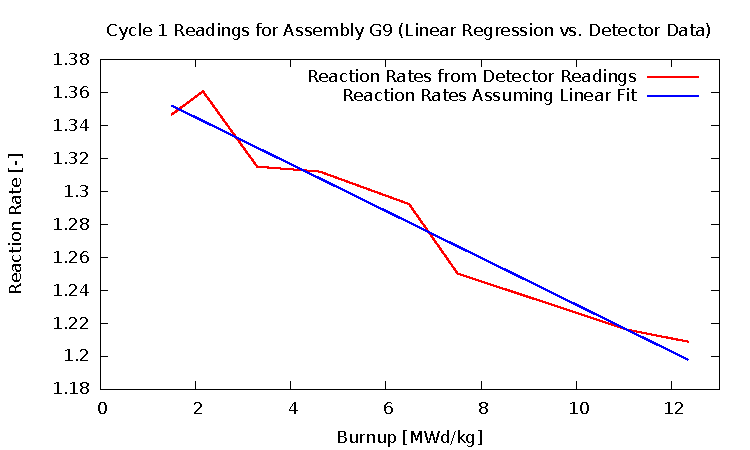
\includegraphics[keepaspectratio, width = 4.5 in]{figures/G9.pdf}
\caption{Cycle 1 measured and linearly regressed reaction rates vs. burnup for assembly G9.}
\label{fig:lm_G9}
\end{figure}

\definecolor{Dfourteencolor}{rgb}{1,1,1}
\definecolor{Ntwocolor}{rgb}{1,1,1}
\definecolor{Gsevencolor}{rgb}{1,1,1}
\definecolor{Gsixcolor}{rgb}{1,1,1}
\definecolor{Gfivecolor}{rgb}{1,1,1}
\definecolor{Gfourcolor}{rgb}{1,1,1}
\definecolor{Gthreecolor}{rgb}{1,1,1}
\definecolor{Gtwocolor}{rgb}{1,1,1}
\definecolor{Gonecolor}{rgb}{1,1,1}
\definecolor{Nfourcolor}{rgb}{1,1,1}
\definecolor{Kfourteencolor}{rgb}{1,1,1}
\definecolor{Gninecolor}{rgb}{0.788937308509,0.8,0.16}
\definecolor{Geightcolor}{rgb}{0.8,0.487862712607,0.16}
\definecolor{Nsixcolor}{rgb}{1,1,1}
\definecolor{Nsevencolor}{rgb}{1,1,1}
\definecolor{Rfivecolor}{rgb}{1,1,1}
\definecolor{Rsixcolor}{rgb}{1,1,1}
\definecolor{Rsevencolor}{rgb}{1,1,1}
\definecolor{Reightcolor}{rgb}{1,1,1}
\definecolor{Rninecolor}{rgb}{1,1,1}
\definecolor{Jeightcolor}{rgb}{1,1,1}
\definecolor{Jninecolor}{rgb}{1,1,1}
\definecolor{Jfourcolor}{rgb}{1,1,1}
\definecolor{Jfivecolor}{rgb}{1,1,1}
\definecolor{Jsixcolor}{rgb}{1,1,1}
\definecolor{Jsevencolor}{rgb}{1,1,1}
\definecolor{Jonecolor}{rgb}{1,1,1}
\definecolor{Jtwocolor}{rgb}{1,1,1}
\definecolor{Jthreecolor}{rgb}{1,1,1}
\definecolor{Bfourcolor}{rgb}{1,1,1}
\definecolor{Bfivecolor}{rgb}{1,1,1}
\definecolor{Bsixcolor}{rgb}{1,1,1}
\definecolor{Bsevencolor}{rgb}{1,1,1}
\definecolor{Bthreecolor}{rgb}{1,1,1}
\definecolor{Ksevencolor}{rgb}{1,1,1}
\definecolor{Beightcolor}{rgb}{0.733607992214,0.8,0.16}
\definecolor{Bninecolor}{rgb}{0.198182787233,0.8,0.16}
\definecolor{Ksixcolor}{rgb}{1,1,1}
\definecolor{Nfivecolor}{rgb}{1,1,1}
\definecolor{Kfivecolor}{rgb}{1,1,1}
\definecolor{Lfourteencolor}{rgb}{1,1,1}
\definecolor{Lfifteencolor}{rgb}{1,1,1}
\definecolor{Kfourcolor}{rgb}{1,1,1}
\definecolor{Ltencolor}{rgb}{1,1,1}
\definecolor{Lelevencolor}{rgb}{1,1,1}
\definecolor{Ltwelvecolor}{rgb}{1,1,1}
\definecolor{Lthirteencolor}{rgb}{1,1,1}
\definecolor{Mfivecolor}{rgb}{1,1,1}
\definecolor{Mfourcolor}{rgb}{1,1,1}
\definecolor{Msevencolor}{rgb}{1,1,1}
\definecolor{Msixcolor}{rgb}{1,1,1}
\definecolor{Mthreecolor}{rgb}{1,1,1}
\definecolor{Mtwocolor}{rgb}{1,1,1}
\definecolor{Mninecolor}{rgb}{1,1,1}
\definecolor{Meightcolor}{rgb}{1,1,1}
\definecolor{Rtencolor}{rgb}{1,1,1}
\definecolor{Relevencolor}{rgb}{1,1,1}
\definecolor{Mfourteencolor}{rgb}{1,1,1}
\definecolor{Ptencolor}{rgb}{1,1,1}
\definecolor{Pelevencolor}{rgb}{1,1,1}
\definecolor{Ptwelvecolor}{rgb}{1,1,1}
\definecolor{Pthirteencolor}{rgb}{1,1,1}
\definecolor{Eninecolor}{rgb}{0.8,0.16,0.16}
\definecolor{Eeightcolor}{rgb}{0.458089093855,0.8,0.16}
\definecolor{Efivecolor}{rgb}{1,1,1}
\definecolor{Efourcolor}{rgb}{1,1,1}
\definecolor{Esevencolor}{rgb}{1,1,1}
\definecolor{Esixcolor}{rgb}{1,1,1}
\definecolor{Eonecolor}{rgb}{1,1,1}
\definecolor{Peightcolor}{rgb}{1,1,1}
\definecolor{Ethreecolor}{rgb}{1,1,1}
\definecolor{Etwocolor}{rgb}{1,1,1}
\definecolor{Pthreecolor}{rgb}{1,1,1}
\definecolor{Pninecolor}{rgb}{1,1,1}
\definecolor{Psixcolor}{rgb}{1,1,1}
\definecolor{Psevencolor}{rgb}{1,1,1}
\definecolor{Pfourcolor}{rgb}{1,1,1}
\definecolor{Pfivecolor}{rgb}{1,1,1}
\definecolor{Htencolor}{rgb}{1,1,1}
\definecolor{Helevencolor}{rgb}{1,1,1}
\definecolor{Htwelvecolor}{rgb}{1,1,1}
\definecolor{Hthirteencolor}{rgb}{1,1,1}
\definecolor{Hfourteencolor}{rgb}{1,1,1}
\definecolor{Hfifteencolor}{rgb}{1,1,1}
\definecolor{Ftwelvecolor}{rgb}{1,1,1}
\definecolor{Fthirteencolor}{rgb}{1,1,1}
\definecolor{Ftencolor}{rgb}{0.8,0.681558463886,0.16}
\definecolor{Felevencolor}{rgb}{1,1,1}
\definecolor{Ffourteencolor}{rgb}{1,1,1}
\definecolor{Ffifteencolor}{rgb}{1,1,1}
\definecolor{Ntwelvecolor}{rgb}{1,1,1}
\definecolor{Nthirteencolor}{rgb}{1,1,1}
\definecolor{Heightcolor}{rgb}{1,1,1}
\definecolor{Nelevencolor}{rgb}{1,1,1}
\definecolor{Nfourteencolor}{rgb}{1,1,1}
\definecolor{Htwocolor}{rgb}{1,1,1}
\definecolor{Hthreecolor}{rgb}{1,1,1}
\definecolor{Honecolor}{rgb}{1,1,1}
\definecolor{Hsixcolor}{rgb}{1,1,1}
\definecolor{Hsevencolor}{rgb}{1,1,1}
\definecolor{Hfourcolor}{rgb}{1,1,1}
\definecolor{Hfivecolor}{rgb}{1,1,1}
\definecolor{Kthirteencolor}{rgb}{1,1,1}
\definecolor{Ktwelvecolor}{rgb}{1,1,1}
\definecolor{Kelevencolor}{rgb}{1,1,1}
\definecolor{Ktencolor}{rgb}{1,1,1}
\definecolor{Dtencolor}{rgb}{0.369407255626,0.8,0.16}
\definecolor{Delevencolor}{rgb}{1,1,1}
\definecolor{Dtwelvecolor}{rgb}{0.8,0.596264260559,0.16}
\definecolor{Dthirteencolor}{rgb}{1,1,1}
\definecolor{Kthreecolor}{rgb}{1,1,1}
\definecolor{Ktwocolor}{rgb}{1,1,1}
\definecolor{Konecolor}{rgb}{1,1,1}
\definecolor{Btwelvecolor}{rgb}{0.306283503082,0.8,0.16}
\definecolor{Bthirteencolor}{rgb}{0.335293250138,0.8,0.16}
\definecolor{Btencolor}{rgb}{0.754212258812,0.8,0.16}
\definecolor{Belevencolor}{rgb}{1,1,1}
\definecolor{Kninecolor}{rgb}{1,1,1}
\definecolor{Keightcolor}{rgb}{1,1,1}
\definecolor{Nthreecolor}{rgb}{1,1,1}
\definecolor{Cninecolor}{rgb}{0.736783848638,0.8,0.16}
\definecolor{Ceightcolor}{rgb}{0.8,0.775784852949,0.16}
\definecolor{Cthreecolor}{rgb}{1,1,1}
\definecolor{Ctwocolor}{rgb}{1,1,1}
\definecolor{Kfifteencolor}{rgb}{1,1,1}
\definecolor{Jfifteencolor}{rgb}{1,1,1}
\definecolor{Csevencolor}{rgb}{1,1,1}
\definecolor{Csixcolor}{rgb}{1,1,1}
\definecolor{Cfivecolor}{rgb}{1,1,1}
\definecolor{Cfourcolor}{rgb}{1,1,1}
\definecolor{Etwelvecolor}{rgb}{1,1,1}
\definecolor{Ntencolor}{rgb}{1,1,1}
\definecolor{Neightcolor}{rgb}{1,1,1}
\definecolor{Nninecolor}{rgb}{1,1,1}
\definecolor{Hninecolor}{rgb}{1,1,1}
\definecolor{Gfifteencolor}{rgb}{1,1,1}
\definecolor{Gfourteencolor}{rgb}{1,1,1}
\definecolor{Gthirteencolor}{rgb}{1,1,1}
\definecolor{Gtwelvecolor}{rgb}{1,1,1}
\definecolor{Gelevencolor}{rgb}{1,1,1}
\definecolor{Gtencolor}{rgb}{1,1,1}
\definecolor{Fonecolor}{rgb}{1,1,1}
\definecolor{Ftwocolor}{rgb}{1,1,1}
\definecolor{Fthreecolor}{rgb}{1,1,1}
\definecolor{Ffourcolor}{rgb}{1,1,1}
\definecolor{Ffivecolor}{rgb}{1,1,1}
\definecolor{Fsixcolor}{rgb}{1,1,1}
\definecolor{Fsevencolor}{rgb}{1,1,1}
\definecolor{Feightcolor}{rgb}{0.8,0.447567164027,0.16}
\definecolor{Fninecolor}{rgb}{0.67362541086,0.8,0.16}
\definecolor{Jthirteencolor}{rgb}{1,1,1}
\definecolor{Melevencolor}{rgb}{1,1,1}
\definecolor{Mtencolor}{rgb}{1,1,1}
\definecolor{Mthirteencolor}{rgb}{1,1,1}
\definecolor{Mtwelvecolor}{rgb}{1,1,1}
\definecolor{Jtencolor}{rgb}{1,1,1}
\definecolor{Jelevencolor}{rgb}{1,1,1}
\definecolor{Eelevencolor}{rgb}{0.38322722713,0.8,0.16}
\definecolor{Etencolor}{rgb}{0.651865606061,0.8,0.16}
\definecolor{Ethirteencolor}{rgb}{1,1,1}
\definecolor{Jfourteencolor}{rgb}{1,1,1}
\definecolor{Efifteencolor}{rgb}{1,1,1}
\definecolor{Efourteencolor}{rgb}{1,1,1}
\definecolor{Cthirteencolor}{rgb}{0.709174691536,0.8,0.16}
\definecolor{Ctwelvecolor}{rgb}{0.16,0.8,0.16}
\definecolor{Celevencolor}{rgb}{0.248047693761,0.8,0.16}
\definecolor{Ctencolor}{rgb}{0.744971912225,0.8,0.16}
\definecolor{Cfourteencolor}{rgb}{1,1,1}
\definecolor{Aelevencolor}{rgb}{0.272258981518,0.8,0.16}
\definecolor{Atencolor}{rgb}{0.251304698671,0.8,0.16}
\definecolor{Afivecolor}{rgb}{1,1,1}
\definecolor{Asevencolor}{rgb}{1,1,1}
\definecolor{Asixcolor}{rgb}{1,1,1}
\definecolor{Aninecolor}{rgb}{0.435544444217,0.8,0.16}
\definecolor{Aeightcolor}{rgb}{0.519632402613,0.8,0.16}
\definecolor{Jtwelvecolor}{rgb}{1,1,1}
\definecolor{Lsixcolor}{rgb}{1,1,1}
\definecolor{Lsevencolor}{rgb}{1,1,1}
\definecolor{Lfourcolor}{rgb}{1,1,1}
\definecolor{Lfivecolor}{rgb}{1,1,1}
\definecolor{Ltwocolor}{rgb}{1,1,1}
\definecolor{Lthreecolor}{rgb}{1,1,1}
\definecolor{Lonecolor}{rgb}{1,1,1}
\definecolor{Leightcolor}{rgb}{1,1,1}
\definecolor{Lninecolor}{rgb}{1,1,1}
\definecolor{Deightcolor}{rgb}{0.8,0.674789526377,0.16}
\definecolor{Dninecolor}{rgb}{0.8,0.720080143064,0.16}
\definecolor{Dsixcolor}{rgb}{1,1,1}
\definecolor{Dsevencolor}{rgb}{1,1,1}
\definecolor{Dfourcolor}{rgb}{1,1,1}
\definecolor{Dfivecolor}{rgb}{1,1,1}
\definecolor{Dtwocolor}{rgb}{1,1,1}
\definecolor{Dthreecolor}{rgb}{1,1,1}

\begin{figure}[htbp]
    \centering
    
    % these dimensions are determined in arrow_dimms.ods
    
    \def\scale{2.0}

    \def\latWidth{0.2673473684*\scale}
    
    \def\RPVOR{3*\scale}
    \def\rectW{0.75*\scale}
    \def\RPVIR{2.7315789474*\scale}
    \def\BarrelIR{2.3368421053*\scale}
    \def\BarrelOR{2.4078947368*\scale}
    \def\ShieldIR{2.4223787816*\scale}
    \def\ShieldOR{2.5067965189*\scale}
    \def\LinerIR{2.7246166598*\scale}

    \def\bafCIRx{0.9357157895*\scale}
    \def\bafCIRy{2.0051052632*\scale}
    \def\bafCORx{0.9633473684*\scale}
    \def\bafCORy{2.0327368421*\scale}
    \def\bafMIRx{1.7377578947*\scale}
    \def\bafMIRy{1.4704105263*\scale}
    \def\bafMORx{1.7653894737*\scale}
    \def\bafMORy{1.4980421053*\scale}
    
    \tikzset{Assembly/.style={
        inner sep=0pt,
        text width=\latWidth in,
        minimum size=\latWidth in,
        draw=black,
        align=center
        }
    }
    
    \def\tkzRPV{(0,0) circle (\RPVIR) (0,0) circle (\RPVOR)}
    \def\tkzLiner{(0,0) circle (\LinerIR) (0,0) circle (\RPVIR)}
    \def\tkzBarrel{(0,0) circle (\BarrelIR) (0,0) circle (\BarrelOR)}
    \def\tkzShields{(0,0) circle (\ShieldIR) (0,0) circle (\ShieldOR)}
    
    \def\tkzBaffCOR{(-\bafCORx, -\bafCORy) rectangle (\bafCORx, \bafCORy)}
    \def\tkzBaffCIR{(-\bafCIRx, -\bafCIRy) rectangle (\bafCIRx, \bafCIRy)} 
    \def\tkzBaffMOR{(-\bafMORx, -\bafMORy) rectangle (\bafMORx, \bafMORy)}
    \def\tkzBaffMIR{(-\bafMIRx, -\bafMIRy) rectangle (\bafMIRx, \bafMIRy) }
    \def\tkzBaffleC{ \tkzBaffCIR \tkzBaffCOR }
    \def\tkzBaffleM{ \tkzBaffMIR \tkzBaffMOR }

    \def\tkzBaffCClip{\tkzBaffCIR (-\RPVOR, -\RPVOR) rectangle (\RPVOR, \RPVOR)}
    \def\tkzBaffMClip{\tkzBaffMIR (-\RPVOR, -\RPVOR) rectangle (\RPVOR, \RPVOR)}

    \def\highenr{blue!50}
    \def\midenr{yellow!50}
    \def\lowenr{red!50}
    
    \scalebox{0.6}{
    
      \begin{tikzpicture}[x=1in,y=1in]
      \fontfamily{mdbch}\selectfont
        %\begin{scope}
          %\clip ($(-\latWidth/2,\latWidth/2)$) rectangle (\RPVOR,-\RPVOR);
          % draw RPV, barrel, and shield panels
          
          %\path[fill=black!90!white,even odd rule] \tkzRPV;
          %\path[fill=black,even odd rule] \tkzLiner;
          %\path[fill=black,even odd rule] \tkzBarrel;
          %\begin{scope}
          %  \clip (0,0) -- +(61:\RPVOR) arc (61:29:\RPVOR) --
          %        (0,0) -- +(151:\RPVOR) arc (151:119:\RPVOR) -- 
          %        (0,0) -- +(241:\RPVOR) arc (241:209:\RPVOR) -- 
          %        (0,0) -- +(331:\RPVOR) arc (331:299:\RPVOR) -- cycle;
          %  \path[fill=black,even odd rule] \tkzShields;
          %\end{scope}

          % draw baffle north/south
          
          %\begin{scope}[even odd rule]
          %  \clip[rotate=90] \tkzBaffMClip;
          %  \path[fill=black] \tkzBaffleC;
          %\end{scope}
          %\begin{scope}[even odd rule]
          %  \clip \tkzBaffCClip;
          %  \clip \tkzBaffMClip;
          %  \path[fill=black, rotate=90] \tkzBaffleM;
          %\end{scope}
          
          % draw baffle east/west
          
          %\begin{scope}[rotate=90]
          %  \begin{scope}[even odd rule]
          %    \clip[rotate=90] \tkzBaffMClip;
          %    \path[fill=black] \tkzBaffleC;
          %  \end{scope}
          %  \begin{scope}[even odd rule]
          %    \clip \tkzBaffCClip;
          %    \clip \tkzBaffMClip;
          %    \path[fill=black, rotate=90] \tkzBaffleM;
          %  \end{scope}
          %\end{scope}
          
        %\end{scope}
        
        % draw assembly row/column headers
        
        \draw[red, thick] ($(-0*\latWidth,1*\latWidth)$) node[above, anchor=south] {H} -- ($(-0*\latWidth,0.6*\latWidth)$);
        \draw[red, thick] ($(1*\latWidth,1*\latWidth)$) node[above, anchor=south] {G} -- ($(1*\latWidth,0.6*\latWidth)$);
        \draw[red, thick] ($(2*\latWidth,1*\latWidth)$) node[above, anchor=south] {F} -- ($(2*\latWidth,0.6*\latWidth)$);
        \draw[red, thick] ($(3*\latWidth,1*\latWidth)$) node[above, anchor=south] {E} -- ($(3*\latWidth,0.6*\latWidth)$);
        \draw[red, thick] ($(4*\latWidth,1*\latWidth)$) node[above, anchor=south] {D} -- ($(4*\latWidth,0.6*\latWidth)$);
        \draw[red, thick] ($(5*\latWidth,1*\latWidth)$) node[above, anchor=south] {C} -- ($(5*\latWidth,0.6*\latWidth)$);
        \draw[red, thick] ($(6*\latWidth,1*\latWidth)$) node[above, anchor=south] {B} -- ($(6*\latWidth,0.6*\latWidth)$);
        \draw[red, thick] ($(7*\latWidth,1*\latWidth)$) node[above, anchor=south] {A} -- ($(7*\latWidth,0.6*\latWidth)$);
        
        \begin{scope}[rotate=90]
          \draw[red, thick] ($(-7*\latWidth,1*\latWidth)$) node[left, anchor=east] {15} -- ($(-7*\latWidth,0.6*\latWidth)$);
          \draw[red, thick] ($(-6*\latWidth,1*\latWidth)$) node[left, anchor=east] {14} -- ($(-6*\latWidth,0.6*\latWidth)$);
          \draw[red, thick] ($(-5*\latWidth,1*\latWidth)$) node[left, anchor=east] {13} -- ($(-5*\latWidth,0.6*\latWidth)$);
          \draw[red, thick] ($(-4*\latWidth,1*\latWidth)$) node[left, anchor=east] {12} -- ($(-4*\latWidth,0.6*\latWidth)$);
          \draw[red, thick] ($(-3*\latWidth,1*\latWidth)$) node[left, anchor=east] {11} -- ($(-3*\latWidth,0.6*\latWidth)$);
          \draw[red, thick] ($(-2*\latWidth,1*\latWidth)$) node[left, anchor=east] {10} -- ($(-2*\latWidth,0.6*\latWidth)$);
          \draw[red, thick] ($(-1*\latWidth,1*\latWidth)$) node[left, anchor=east] {9} -- ($(-1*\latWidth,0.6*\latWidth)$);
          \draw[red, thick] ($(-0*\latWidth,1*\latWidth)$) node[left, anchor=east] {8} -- ($(-0*\latWidth,0.6*\latWidth)$);
        \end{scope}
        
        % draw fuel assembly nodes

        \node [Assembly, fill=Heightcolor] at ($(-0*\latWidth,0*\latWidth)$) {}; % H8
        \node [Assembly, fill=Geightcolor] at ($( 1*\latWidth,0*\latWidth)$) {

\scriptsize{0.011} 
 \scriptsize{0.016} 

}; % G8
        \node [Assembly, fill=Feightcolor] at ($( 2*\latWidth,0*\latWidth)$) {

\scriptsize{0.012} 
 \scriptsize{0.941} 

}; % F8
        \node [Assembly, fill=Eeightcolor] at ($( 3*\latWidth,0*\latWidth)$) {

\scriptsize{0.006} 
 \scriptsize{0.949} 

}; % E8
        \node [Assembly, fill=Deightcolor] at ($( 4*\latWidth,0*\latWidth)$) {

\scriptsize{0.010} 
 \scriptsize{0.874} 

}; % D8
        \node [Assembly, fill=Ceightcolor] at ($( 5*\latWidth,0*\latWidth)$) {

\scriptsize{0.009} 
 \scriptsize{0.878} 

}; % C8
        \node [Assembly, fill=Beightcolor] at ($( 6*\latWidth,0*\latWidth)$) {

\scriptsize{0.008} 
 \scriptsize{0.450} 

}; % B8
        \node [Assembly, fill=Aeightcolor] at ($( 7*\latWidth,0*\latWidth)$) {

\scriptsize{0.007} 
 \scriptsize{0.849} 

}; % A8

        \node [Assembly, fill=Hninecolor] at ($(-0*\latWidth,-1*\latWidth)$) {}; % H9
        \node [Assembly, fill=Gninecolor] at ($( 1*\latWidth,-1*\latWidth)$) {

\scriptsize{0.009} 
 \scriptsize{0.955} 

}; % G9
        \node [Assembly, fill=Fninecolor] at ($( 2*\latWidth,-1*\latWidth)$) {

\scriptsize{0.008} 
 \scriptsize{0.926} 

}; % F9
        \node [Assembly, fill=Eninecolor] at ($( 3*\latWidth,-1*\latWidth)$) {

\scriptsize{0.014} 
 \scriptsize{0.921} 

}; % E9
        \node [Assembly, fill=Dninecolor] at ($( 4*\latWidth,-1*\latWidth)$) {

\scriptsize{0.009} 
 \scriptsize{0.260} 

}; % D9
        \node [Assembly, fill=Cninecolor] at ($( 5*\latWidth,-1*\latWidth)$) {

\scriptsize{0.008} 
 \scriptsize{0.348} 

}; % C9
        \node [Assembly, fill=Bninecolor] at ($( 6*\latWidth,-1*\latWidth)$) {

\scriptsize{0.004} 
 \scriptsize{0.992} 

}; % B9
        \node [Assembly, fill=Aninecolor] at ($( 7*\latWidth,-1*\latWidth)$) {

\scriptsize{0.006} 
 \scriptsize{0.862} 

}; % A9

        \node [Assembly, fill=Htencolor] at ($(-0*\latWidth,-2*\latWidth)$) {}; % H10
        \node [Assembly, fill=Gtencolor] at ($( 1*\latWidth,-2*\latWidth)$) {}; % G10
        \node [Assembly, fill=Ftencolor] at ($( 2*\latWidth,-2*\latWidth)$) {

\scriptsize{0.010} 
 \scriptsize{0.960} 

}; % F10
        \node [Assembly, fill=Etencolor] at ($( 3*\latWidth,-2*\latWidth)$) {

\scriptsize{0.008} 
 \scriptsize{0.781} 

}; % E10
        \node [Assembly, fill=Dtencolor] at ($( 4*\latWidth,-2*\latWidth)$) {

\scriptsize{0.006} 
 \scriptsize{0.874} 

}; % D10
        \node [Assembly, fill=Ctencolor] at ($( 5*\latWidth,-2*\latWidth)$) {

\scriptsize{0.008} 
 \scriptsize{0.924} 

}; % C10
        \node [Assembly, fill=Btencolor] at ($( 6*\latWidth,-2*\latWidth)$) {

\scriptsize{0.008} 
 \scriptsize{0.569} 

}; % B10
        \node [Assembly, fill=Atencolor] at ($( 7*\latWidth,-2*\latWidth)$) {

\scriptsize{0.005} 
 \scriptsize{0.968} 

}; % A10

        \node [Assembly, fill=Helevencolor] at ($(-0*\latWidth,-3*\latWidth)$) {}; % H11
        \node [Assembly, fill=Gelevencolor] at ($( 1*\latWidth,-3*\latWidth)$) {}; % G11
        \node [Assembly, fill=Felevencolor] at ($( 2*\latWidth,-3*\latWidth)$) {}; % F11
        \node [Assembly, fill=Eelevencolor] at ($( 3*\latWidth,-3*\latWidth)$) {

\scriptsize{0.006} 
 \scriptsize{0.944} 

}; % E11
        \node [Assembly, fill=Delevencolor] at ($( 4*\latWidth,-3*\latWidth)$) {}; % D11
        \node [Assembly, fill=Celevencolor] at ($( 5*\latWidth,-3*\latWidth)$) {

\scriptsize{0.005} 
 \scriptsize{0.740} 

}; % C11
        \node [Assembly, fill=Belevencolor] at ($( 6*\latWidth,-3*\latWidth)$) {}; % B11
        \node [Assembly, fill=Aelevencolor] at ($( 7*\latWidth,-3*\latWidth)$) {

\scriptsize{0.005} 
 \scriptsize{0.980} 

}; % A11

        \node [Assembly, fill=Htwelvecolor] at ($(-0*\latWidth,-4*\latWidth)$) {}; % H12
        \node [Assembly, fill=Gtwelvecolor] at ($( 1*\latWidth,-4*\latWidth)$) {}; % G12
        \node [Assembly, fill=Ftwelvecolor] at ($( 2*\latWidth,-4*\latWidth)$) {}; % F12
        \node [Assembly, fill=Etwelvecolor] at ($( 3*\latWidth,-4*\latWidth)$) {}; % E12
        \node [Assembly, fill=Dtwelvecolor] at ($( 4*\latWidth,-4*\latWidth)$) {

\scriptsize{0.010} 
 \scriptsize{0.650} 

}; % D12
        \node [Assembly, fill=Ctwelvecolor] at ($( 5*\latWidth,-4*\latWidth)$) {

\scriptsize{0.004} 
 \scriptsize{0.991} 

}; % C12
        \node [Assembly, fill=Btwelvecolor] at ($( 6*\latWidth,-4*\latWidth)$) {

\scriptsize{0.005} 
 \scriptsize{0.906} 

}; % B12

        \node [Assembly, fill=Hthirteencolor] at ($(-0*\latWidth,-5*\latWidth)$) {}; % H13
        \node [Assembly, fill=Gthirteencolor] at ($( 1*\latWidth,-5*\latWidth)$) {}; % G13
        \node [Assembly, fill=Fthirteencolor] at ($( 2*\latWidth,-5*\latWidth)$) {}; % F13
        \node [Assembly, fill=Ethirteencolor] at ($( 3*\latWidth,-5*\latWidth)$) {}; % E13
        \node [Assembly, fill=Dthirteencolor] at ($( 4*\latWidth,-5*\latWidth)$) {}; % D13
        \node [Assembly, fill=Cthirteencolor] at ($( 5*\latWidth,-5*\latWidth)$) {

\scriptsize{0.008} 
 \scriptsize{0.985} 

}; % C13
        \node [Assembly, fill=Bthirteencolor] at ($( 6*\latWidth,-5*\latWidth)$) {

\scriptsize{0.005} 
 \scriptsize{0.956} 

}; % B13

        \node [Assembly, fill=Hfourteencolor] at ($(-0*\latWidth,-6*\latWidth)$) {}; % H14
        \node [Assembly, fill=Gfourteencolor] at ($( 1*\latWidth,-6*\latWidth)$) {}; % G14
        \node [Assembly, fill=Ffourteencolor] at ($( 2*\latWidth,-6*\latWidth)$) {}; % F14
        \node [Assembly, fill=Efourteencolor] at ($( 3*\latWidth,-6*\latWidth)$) {}; % E14
        \node [Assembly, fill=Dfourteencolor] at ($( 4*\latWidth,-6*\latWidth)$) {}; % D14
        \node [Assembly, fill=Cfourteencolor] at ($( 5*\latWidth,-6*\latWidth)$) {}; % C14

        \node [Assembly, fill=Hfifteencolor] at ($(-0*\latWidth,-7*\latWidth)$) {}; % H15
        \node [Assembly, fill=Gfifteencolor] at ($( 1*\latWidth,-7*\latWidth)$) {}; % G15
        \node [Assembly, fill=Ffifteencolor] at ($( 2*\latWidth,-7*\latWidth)$) {}; % F15
        \node [Assembly, fill=Efifteencolor] at ($( 3*\latWidth,-7*\latWidth)$) {}; % E15
        
      \end{tikzpicture}
    }
    


    \caption{Cycle 1 RMS (top) and R-Squared (bottom) values based on applying linear model to data set of reaction rate vs. burnup for each assembly. Assembly-weighted total RMS = 0.008. \label{fig:cyc1_lm_eighth_map}}
\end{figure}


\definecolor{Dfourteencolor}{rgb}{1,1,1}
\definecolor{Ntwocolor}{rgb}{1,1,1}
\definecolor{Gsevencolor}{rgb}{1,1,1}
\definecolor{Gsixcolor}{rgb}{1,1,1}
\definecolor{Gfivecolor}{rgb}{1,1,1}
\definecolor{Gfourcolor}{rgb}{1,1,1}
\definecolor{Gthreecolor}{rgb}{1,1,1}
\definecolor{Gtwocolor}{rgb}{1,1,1}
\definecolor{Gonecolor}{rgb}{1,1,1}
\definecolor{Nfourcolor}{rgb}{1,1,1}
\definecolor{Kfourteencolor}{rgb}{1,1,1}
\definecolor{Gninecolor}{rgb}{0.8,0.480994014531,0.16}
\definecolor{Geightcolor}{rgb}{0.8,0.434570504845,0.16}
\definecolor{Nsixcolor}{rgb}{1,1,1}
\definecolor{Nsevencolor}{rgb}{1,1,1}
\definecolor{Rfivecolor}{rgb}{1,1,1}
\definecolor{Rsixcolor}{rgb}{1,1,1}
\definecolor{Rsevencolor}{rgb}{1,1,1}
\definecolor{Reightcolor}{rgb}{1,1,1}
\definecolor{Rninecolor}{rgb}{1,1,1}
\definecolor{Jeightcolor}{rgb}{1,1,1}
\definecolor{Jninecolor}{rgb}{1,1,1}
\definecolor{Jfourcolor}{rgb}{1,1,1}
\definecolor{Jfivecolor}{rgb}{1,1,1}
\definecolor{Jsixcolor}{rgb}{1,1,1}
\definecolor{Jsevencolor}{rgb}{1,1,1}
\definecolor{Jonecolor}{rgb}{1,1,1}
\definecolor{Jtwocolor}{rgb}{1,1,1}
\definecolor{Jthreecolor}{rgb}{1,1,1}
\definecolor{Bfourcolor}{rgb}{1,1,1}
\definecolor{Bfivecolor}{rgb}{1,1,1}
\definecolor{Bsixcolor}{rgb}{1,1,1}
\definecolor{Bsevencolor}{rgb}{1,1,1}
\definecolor{Bthreecolor}{rgb}{1,1,1}
\definecolor{Ksevencolor}{rgb}{1,1,1}
\definecolor{Beightcolor}{rgb}{0.446024276252,0.8,0.16}
\definecolor{Bninecolor}{rgb}{0.37813653837,0.8,0.16}
\definecolor{Ksixcolor}{rgb}{1,1,1}
\definecolor{Nfivecolor}{rgb}{1,1,1}
\definecolor{Kfivecolor}{rgb}{1,1,1}
\definecolor{Lfourteencolor}{rgb}{1,1,1}
\definecolor{Lfifteencolor}{rgb}{1,1,1}
\definecolor{Kfourcolor}{rgb}{1,1,1}
\definecolor{Ltencolor}{rgb}{1,1,1}
\definecolor{Lelevencolor}{rgb}{1,1,1}
\definecolor{Ltwelvecolor}{rgb}{1,1,1}
\definecolor{Lthirteencolor}{rgb}{1,1,1}
\definecolor{Mfivecolor}{rgb}{1,1,1}
\definecolor{Mfourcolor}{rgb}{1,1,1}
\definecolor{Msevencolor}{rgb}{1,1,1}
\definecolor{Msixcolor}{rgb}{1,1,1}
\definecolor{Mthreecolor}{rgb}{1,1,1}
\definecolor{Mtwocolor}{rgb}{1,1,1}
\definecolor{Mninecolor}{rgb}{1,1,1}
\definecolor{Meightcolor}{rgb}{1,1,1}
\definecolor{Rtencolor}{rgb}{1,1,1}
\definecolor{Relevencolor}{rgb}{1,1,1}
\definecolor{Mfourteencolor}{rgb}{1,1,1}
\definecolor{Ptencolor}{rgb}{1,1,1}
\definecolor{Pelevencolor}{rgb}{1,1,1}
\definecolor{Ptwelvecolor}{rgb}{1,1,1}
\definecolor{Pthirteencolor}{rgb}{1,1,1}
\definecolor{Eninecolor}{rgb}{0.273575861365,0.8,0.16}
\definecolor{Eeightcolor}{rgb}{0.719649388974,0.8,0.16}
\definecolor{Efivecolor}{rgb}{1,1,1}
\definecolor{Efourcolor}{rgb}{1,1,1}
\definecolor{Esevencolor}{rgb}{1,1,1}
\definecolor{Esixcolor}{rgb}{1,1,1}
\definecolor{Eonecolor}{rgb}{1,1,1}
\definecolor{Peightcolor}{rgb}{1,1,1}
\definecolor{Ethreecolor}{rgb}{1,1,1}
\definecolor{Etwocolor}{rgb}{1,1,1}
\definecolor{Pthreecolor}{rgb}{1,1,1}
\definecolor{Pninecolor}{rgb}{1,1,1}
\definecolor{Psixcolor}{rgb}{1,1,1}
\definecolor{Psevencolor}{rgb}{1,1,1}
\definecolor{Pfourcolor}{rgb}{1,1,1}
\definecolor{Pfivecolor}{rgb}{1,1,1}
\definecolor{Htencolor}{rgb}{1,1,1}
\definecolor{Helevencolor}{rgb}{1,1,1}
\definecolor{Htwelvecolor}{rgb}{1,1,1}
\definecolor{Hthirteencolor}{rgb}{1,1,1}
\definecolor{Hfourteencolor}{rgb}{1,1,1}
\definecolor{Hfifteencolor}{rgb}{1,1,1}
\definecolor{Ftwelvecolor}{rgb}{1,1,1}
\definecolor{Fthirteencolor}{rgb}{1,1,1}
\definecolor{Ftencolor}{rgb}{0.290438811543,0.8,0.16}
\definecolor{Felevencolor}{rgb}{1,1,1}
\definecolor{Ffourteencolor}{rgb}{1,1,1}
\definecolor{Ffifteencolor}{rgb}{1,1,1}
\definecolor{Ntwelvecolor}{rgb}{1,1,1}
\definecolor{Nthirteencolor}{rgb}{1,1,1}
\definecolor{Heightcolor}{rgb}{1,1,1}
\definecolor{Nelevencolor}{rgb}{1,1,1}
\definecolor{Nfourteencolor}{rgb}{1,1,1}
\definecolor{Htwocolor}{rgb}{1,1,1}
\definecolor{Hthreecolor}{rgb}{1,1,1}
\definecolor{Honecolor}{rgb}{1,1,1}
\definecolor{Hsixcolor}{rgb}{1,1,1}
\definecolor{Hsevencolor}{rgb}{1,1,1}
\definecolor{Hfourcolor}{rgb}{1,1,1}
\definecolor{Hfivecolor}{rgb}{1,1,1}
\definecolor{Kthirteencolor}{rgb}{1,1,1}
\definecolor{Ktwelvecolor}{rgb}{1,1,1}
\definecolor{Kelevencolor}{rgb}{1,1,1}
\definecolor{Ktencolor}{rgb}{1,1,1}
\definecolor{Dtencolor}{rgb}{0.606771906188,0.8,0.16}
\definecolor{Delevencolor}{rgb}{1,1,1}
\definecolor{Dtwelvecolor}{rgb}{0.8,0.16,0.16}
\definecolor{Dthirteencolor}{rgb}{1,1,1}
\definecolor{Kthreecolor}{rgb}{1,1,1}
\definecolor{Ktwocolor}{rgb}{1,1,1}
\definecolor{Konecolor}{rgb}{1,1,1}
\definecolor{Btwelvecolor}{rgb}{0.591068418664,0.8,0.16}
\definecolor{Bthirteencolor}{rgb}{0.8,0.788858672965,0.16}
\definecolor{Btencolor}{rgb}{0.557643488498,0.8,0.16}
\definecolor{Belevencolor}{rgb}{1,1,1}
\definecolor{Kninecolor}{rgb}{1,1,1}
\definecolor{Keightcolor}{rgb}{1,1,1}
\definecolor{Nthreecolor}{rgb}{1,1,1}
\definecolor{Cninecolor}{rgb}{0.16,0.8,0.16}
\definecolor{Ceightcolor}{rgb}{0.377686844682,0.8,0.16}
\definecolor{Cthreecolor}{rgb}{1,1,1}
\definecolor{Ctwocolor}{rgb}{1,1,1}
\definecolor{Kfifteencolor}{rgb}{1,1,1}
\definecolor{Jfifteencolor}{rgb}{1,1,1}
\definecolor{Csevencolor}{rgb}{1,1,1}
\definecolor{Csixcolor}{rgb}{1,1,1}
\definecolor{Cfivecolor}{rgb}{1,1,1}
\definecolor{Cfourcolor}{rgb}{1,1,1}
\definecolor{Etwelvecolor}{rgb}{1,1,1}
\definecolor{Ntencolor}{rgb}{1,1,1}
\definecolor{Neightcolor}{rgb}{1,1,1}
\definecolor{Nninecolor}{rgb}{1,1,1}
\definecolor{Hninecolor}{rgb}{1,1,1}
\definecolor{Gfifteencolor}{rgb}{1,1,1}
\definecolor{Gfourteencolor}{rgb}{1,1,1}
\definecolor{Gthirteencolor}{rgb}{1,1,1}
\definecolor{Gtwelvecolor}{rgb}{1,1,1}
\definecolor{Gelevencolor}{rgb}{1,1,1}
\definecolor{Gtencolor}{rgb}{1,1,1}
\definecolor{Fonecolor}{rgb}{1,1,1}
\definecolor{Ftwocolor}{rgb}{1,1,1}
\definecolor{Fthreecolor}{rgb}{1,1,1}
\definecolor{Ffourcolor}{rgb}{1,1,1}
\definecolor{Ffivecolor}{rgb}{1,1,1}
\definecolor{Fsixcolor}{rgb}{1,1,1}
\definecolor{Fsevencolor}{rgb}{1,1,1}
\definecolor{Feightcolor}{rgb}{0.8,0.630418639974,0.16}
\definecolor{Fninecolor}{rgb}{0.714450689803,0.8,0.16}
\definecolor{Jthirteencolor}{rgb}{1,1,1}
\definecolor{Melevencolor}{rgb}{1,1,1}
\definecolor{Mtencolor}{rgb}{1,1,1}
\definecolor{Mthirteencolor}{rgb}{1,1,1}
\definecolor{Mtwelvecolor}{rgb}{1,1,1}
\definecolor{Jtencolor}{rgb}{1,1,1}
\definecolor{Jelevencolor}{rgb}{1,1,1}
\definecolor{Eelevencolor}{rgb}{0.8,0.778843143831,0.16}
\definecolor{Etencolor}{rgb}{0.452479207461,0.8,0.16}
\definecolor{Ethirteencolor}{rgb}{1,1,1}
\definecolor{Jfourteencolor}{rgb}{1,1,1}
\definecolor{Efifteencolor}{rgb}{1,1,1}
\definecolor{Efourteencolor}{rgb}{1,1,1}
\definecolor{Cthirteencolor}{rgb}{0.721909211844,0.8,0.16}
\definecolor{Ctwelvecolor}{rgb}{0.685518297706,0.8,0.16}
\definecolor{Celevencolor}{rgb}{0.755129793172,0.8,0.16}
\definecolor{Ctencolor}{rgb}{0.359549466435,0.8,0.16}
\definecolor{Cfourteencolor}{rgb}{1,1,1}
\definecolor{Aelevencolor}{rgb}{0.752275522225,0.8,0.16}
\definecolor{Atencolor}{rgb}{0.508542413421,0.8,0.16}
\definecolor{Afivecolor}{rgb}{1,1,1}
\definecolor{Asevencolor}{rgb}{1,1,1}
\definecolor{Asixcolor}{rgb}{1,1,1}
\definecolor{Aninecolor}{rgb}{0.642641682326,0.8,0.16}
\definecolor{Aeightcolor}{rgb}{0.691344828444,0.8,0.16}
\definecolor{Jtwelvecolor}{rgb}{1,1,1}
\definecolor{Lsixcolor}{rgb}{1,1,1}
\definecolor{Lsevencolor}{rgb}{1,1,1}
\definecolor{Lfourcolor}{rgb}{1,1,1}
\definecolor{Lfivecolor}{rgb}{1,1,1}
\definecolor{Ltwocolor}{rgb}{1,1,1}
\definecolor{Lthreecolor}{rgb}{1,1,1}
\definecolor{Lonecolor}{rgb}{1,1,1}
\definecolor{Leightcolor}{rgb}{1,1,1}
\definecolor{Lninecolor}{rgb}{1,1,1}
\definecolor{Deightcolor}{rgb}{0.333438465784,0.8,0.16}
\definecolor{Dninecolor}{rgb}{0.232335289883,0.8,0.16}
\definecolor{Dsixcolor}{rgb}{1,1,1}
\definecolor{Dsevencolor}{rgb}{1,1,1}
\definecolor{Dfourcolor}{rgb}{1,1,1}
\definecolor{Dfivecolor}{rgb}{1,1,1}
\definecolor{Dtwocolor}{rgb}{1,1,1}
\definecolor{Dthreecolor}{rgb}{1,1,1}

\begin{figure}[htbp]
    \centering
    
    % these dimensions are determined in arrow_dimms.ods
    
    \def\scale{2.0}

    \def\latWidth{0.2673473684*\scale}
    
    \def\RPVOR{3*\scale}
    \def\rectW{0.75*\scale}
    \def\RPVIR{2.7315789474*\scale}
    \def\BarrelIR{2.3368421053*\scale}
    \def\BarrelOR{2.4078947368*\scale}
    \def\ShieldIR{2.4223787816*\scale}
    \def\ShieldOR{2.5067965189*\scale}
    \def\LinerIR{2.7246166598*\scale}

    \def\bafCIRx{0.9357157895*\scale}
    \def\bafCIRy{2.0051052632*\scale}
    \def\bafCORx{0.9633473684*\scale}
    \def\bafCORy{2.0327368421*\scale}
    \def\bafMIRx{1.7377578947*\scale}
    \def\bafMIRy{1.4704105263*\scale}
    \def\bafMORx{1.7653894737*\scale}
    \def\bafMORy{1.4980421053*\scale}
    
    \tikzset{Assembly/.style={
        inner sep=0pt,
        text width=\latWidth in,
        minimum size=\latWidth in,
        draw=black,
        align=center
        }
    }
    
    \def\tkzRPV{(0,0) circle (\RPVIR) (0,0) circle (\RPVOR)}
    \def\tkzLiner{(0,0) circle (\LinerIR) (0,0) circle (\RPVIR)}
    \def\tkzBarrel{(0,0) circle (\BarrelIR) (0,0) circle (\BarrelOR)}
    \def\tkzShields{(0,0) circle (\ShieldIR) (0,0) circle (\ShieldOR)}
    
    \def\tkzBaffCOR{(-\bafCORx, -\bafCORy) rectangle (\bafCORx, \bafCORy)}
    \def\tkzBaffCIR{(-\bafCIRx, -\bafCIRy) rectangle (\bafCIRx, \bafCIRy)} 
    \def\tkzBaffMOR{(-\bafMORx, -\bafMORy) rectangle (\bafMORx, \bafMORy)}
    \def\tkzBaffMIR{(-\bafMIRx, -\bafMIRy) rectangle (\bafMIRx, \bafMIRy) }
    \def\tkzBaffleC{ \tkzBaffCIR \tkzBaffCOR }
    \def\tkzBaffleM{ \tkzBaffMIR \tkzBaffMOR }

    \def\tkzBaffCClip{\tkzBaffCIR (-\RPVOR, -\RPVOR) rectangle (\RPVOR, \RPVOR)}
    \def\tkzBaffMClip{\tkzBaffMIR (-\RPVOR, -\RPVOR) rectangle (\RPVOR, \RPVOR)}

    \def\highenr{blue!50}
    \def\midenr{yellow!50}
    \def\lowenr{red!50}
    
    \scalebox{0.6}{
    
      \begin{tikzpicture}[x=1in,y=1in]
      \fontfamily{mdbch}\selectfont
        %\begin{scope}
          %\clip ($(-\latWidth/2,\latWidth/2)$) rectangle (\RPVOR,-\RPVOR);
          % draw RPV, barrel, and shield panels
          
          %\path[fill=black!90!white,even odd rule] \tkzRPV;
          %\path[fill=black,even odd rule] \tkzLiner;
          %\path[fill=black,even odd rule] \tkzBarrel;
          %\begin{scope}
          %  \clip (0,0) -- +(61:\RPVOR) arc (61:29:\RPVOR) --
          %        (0,0) -- +(151:\RPVOR) arc (151:119:\RPVOR) -- 
          %        (0,0) -- +(241:\RPVOR) arc (241:209:\RPVOR) -- 
          %        (0,0) -- +(331:\RPVOR) arc (331:299:\RPVOR) -- cycle;
          %  \path[fill=black,even odd rule] \tkzShields;
          %\end{scope}

          % draw baffle north/south
          
          %\begin{scope}[even odd rule]
          %  \clip[rotate=90] \tkzBaffMClip;
          %  \path[fill=black] \tkzBaffleC;
          %\end{scope}
          %\begin{scope}[even odd rule]
          %  \clip \tkzBaffCClip;
          %  \clip \tkzBaffMClip;
          %  \path[fill=black, rotate=90] \tkzBaffleM;
          %\end{scope}
          
          % draw baffle east/west
          
          %\begin{scope}[rotate=90]
          %  \begin{scope}[even odd rule]
          %    \clip[rotate=90] \tkzBaffMClip;
          %    \path[fill=black] \tkzBaffleC;
          %  \end{scope}
          %  \begin{scope}[even odd rule]
          %    \clip \tkzBaffCClip;
          %    \clip \tkzBaffMClip;
          %    \path[fill=black, rotate=90] \tkzBaffleM;
          %  \end{scope}
          %\end{scope}
          
        %\end{scope}
        
        % draw assembly row/column headers
        
        \draw[red, thick] ($(-0*\latWidth,1*\latWidth)$) node[above, anchor=south] {H} -- ($(-0*\latWidth,0.6*\latWidth)$);
        \draw[red, thick] ($(1*\latWidth,1*\latWidth)$) node[above, anchor=south] {G} -- ($(1*\latWidth,0.6*\latWidth)$);
        \draw[red, thick] ($(2*\latWidth,1*\latWidth)$) node[above, anchor=south] {F} -- ($(2*\latWidth,0.6*\latWidth)$);
        \draw[red, thick] ($(3*\latWidth,1*\latWidth)$) node[above, anchor=south] {E} -- ($(3*\latWidth,0.6*\latWidth)$);
        \draw[red, thick] ($(4*\latWidth,1*\latWidth)$) node[above, anchor=south] {D} -- ($(4*\latWidth,0.6*\latWidth)$);
        \draw[red, thick] ($(5*\latWidth,1*\latWidth)$) node[above, anchor=south] {C} -- ($(5*\latWidth,0.6*\latWidth)$);
        \draw[red, thick] ($(6*\latWidth,1*\latWidth)$) node[above, anchor=south] {B} -- ($(6*\latWidth,0.6*\latWidth)$);
        \draw[red, thick] ($(7*\latWidth,1*\latWidth)$) node[above, anchor=south] {A} -- ($(7*\latWidth,0.6*\latWidth)$);
        
        \begin{scope}[rotate=90]
          \draw[red, thick] ($(-7*\latWidth,1*\latWidth)$) node[left, anchor=east] {15} -- ($(-7*\latWidth,0.6*\latWidth)$);
          \draw[red, thick] ($(-6*\latWidth,1*\latWidth)$) node[left, anchor=east] {14} -- ($(-6*\latWidth,0.6*\latWidth)$);
          \draw[red, thick] ($(-5*\latWidth,1*\latWidth)$) node[left, anchor=east] {13} -- ($(-5*\latWidth,0.6*\latWidth)$);
          \draw[red, thick] ($(-4*\latWidth,1*\latWidth)$) node[left, anchor=east] {12} -- ($(-4*\latWidth,0.6*\latWidth)$);
          \draw[red, thick] ($(-3*\latWidth,1*\latWidth)$) node[left, anchor=east] {11} -- ($(-3*\latWidth,0.6*\latWidth)$);
          \draw[red, thick] ($(-2*\latWidth,1*\latWidth)$) node[left, anchor=east] {10} -- ($(-2*\latWidth,0.6*\latWidth)$);
          \draw[red, thick] ($(-1*\latWidth,1*\latWidth)$) node[left, anchor=east] {9} -- ($(-1*\latWidth,0.6*\latWidth)$);
          \draw[red, thick] ($(-0*\latWidth,1*\latWidth)$) node[left, anchor=east] {8} -- ($(-0*\latWidth,0.6*\latWidth)$);
        \end{scope}
        
        % draw fuel assembly nodes

        \node [Assembly, fill=Heightcolor] at ($(-0*\latWidth,0*\latWidth)$) {}; % H8
        \node [Assembly, fill=Geightcolor] at ($( 1*\latWidth,0*\latWidth)$) {

\scriptsize{0.017} 
 \scriptsize{0.829} 

}; % G8
        \node [Assembly, fill=Feightcolor] at ($( 2*\latWidth,0*\latWidth)$) {

\scriptsize{0.014} 
 \scriptsize{0.776} 

}; % F8
        \node [Assembly, fill=Eeightcolor] at ($( 3*\latWidth,0*\latWidth)$) {

\scriptsize{0.011} 
 \scriptsize{0.789} 

}; % E8
        \node [Assembly, fill=Deightcolor] at ($( 4*\latWidth,0*\latWidth)$) {

\scriptsize{0.005} 
 \scriptsize{0.160} 

}; % D8
        \node [Assembly, fill=Ceightcolor] at ($( 5*\latWidth,0*\latWidth)$) {

\scriptsize{0.006} 
 \scriptsize{0.768} 

}; % C8
        \node [Assembly, fill=Beightcolor] at ($( 6*\latWidth,0*\latWidth)$) {

\scriptsize{0.007} 
 \scriptsize{0.888} 

}; % B8
        \node [Assembly, fill=Aeightcolor] at ($( 7*\latWidth,0*\latWidth)$) {

\scriptsize{0.010} 
 \scriptsize{0.964} 

}; % A8

        \node [Assembly, fill=Hninecolor] at ($(-0*\latWidth,-1*\latWidth)$) {}; % H9
        \node [Assembly, fill=Gninecolor] at ($( 1*\latWidth,-1*\latWidth)$) {

\scriptsize{0.016} 
 \scriptsize{0.781} 

}; % G9
        \node [Assembly, fill=Fninecolor] at ($( 2*\latWidth,-1*\latWidth)$) {

\scriptsize{0.011} 
 \scriptsize{0.848} 

}; % F9
        \node [Assembly, fill=Eninecolor] at ($( 3*\latWidth,-1*\latWidth)$) {

\scriptsize{0.004} 
 \scriptsize{0.021} 

}; % E9
        \node [Assembly, fill=Dninecolor] at ($( 4*\latWidth,-1*\latWidth)$) {

\scriptsize{0.004} 
 \scriptsize{0.476} 

}; % D9
        \node [Assembly, fill=Cninecolor] at ($( 5*\latWidth,-1*\latWidth)$) {

\scriptsize{0.003} 
 \scriptsize{0.065} 

}; % C9
        \node [Assembly, fill=Bninecolor] at ($( 6*\latWidth,-1*\latWidth)$) {

\scriptsize{0.006} 
 \scriptsize{0.640} 

}; % B9
        \node [Assembly, fill=Aninecolor] at ($( 7*\latWidth,-1*\latWidth)$) {

\scriptsize{0.010} 
 \scriptsize{0.967} 

}; % A9

        \node [Assembly, fill=Htencolor] at ($(-0*\latWidth,-2*\latWidth)$) {}; % H10
        \node [Assembly, fill=Gtencolor] at ($( 1*\latWidth,-2*\latWidth)$) {}; % G10
        \node [Assembly, fill=Ftencolor] at ($( 2*\latWidth,-2*\latWidth)$) {

\scriptsize{0.005} 
 \scriptsize{0.609} 

}; % F10
        \node [Assembly, fill=Etencolor] at ($( 3*\latWidth,-2*\latWidth)$) {

\scriptsize{0.007} 
 \scriptsize{0.457} 

}; % E10
        \node [Assembly, fill=Dtencolor] at ($( 4*\latWidth,-2*\latWidth)$) {

\scriptsize{0.009} 
 \scriptsize{0.927} 

}; % D10
        \node [Assembly, fill=Ctencolor] at ($( 5*\latWidth,-2*\latWidth)$) {

\scriptsize{0.006} 
 \scriptsize{0.758} 

}; % C10
        \node [Assembly, fill=Btencolor] at ($( 6*\latWidth,-2*\latWidth)$) {

\scriptsize{0.008} 
 \scriptsize{0.185} 

}; % B10
        \node [Assembly, fill=Atencolor] at ($( 7*\latWidth,-2*\latWidth)$) {

\scriptsize{0.008} 
 \scriptsize{0.907} 

}; % A10

        \node [Assembly, fill=Helevencolor] at ($(-0*\latWidth,-3*\latWidth)$) {}; % H11
        \node [Assembly, fill=Gelevencolor] at ($( 1*\latWidth,-3*\latWidth)$) {}; % G11
        \node [Assembly, fill=Felevencolor] at ($( 2*\latWidth,-3*\latWidth)$) {}; % F11
        \node [Assembly, fill=Eelevencolor] at ($( 3*\latWidth,-3*\latWidth)$) {

\scriptsize{0.012} 
 \scriptsize{0.947} 

}; % E11
        \node [Assembly, fill=Delevencolor] at ($( 4*\latWidth,-3*\latWidth)$) {}; % D11
        \node [Assembly, fill=Celevencolor] at ($( 5*\latWidth,-3*\latWidth)$) {

\scriptsize{0.011} 
 \scriptsize{0.898} 

}; % C11
        \node [Assembly, fill=Belevencolor] at ($( 6*\latWidth,-3*\latWidth)$) {}; % B11
        \node [Assembly, fill=Aelevencolor] at ($( 7*\latWidth,-3*\latWidth)$) {

\scriptsize{0.011} 
 \scriptsize{0.936} 

}; % A11

        \node [Assembly, fill=Htwelvecolor] at ($(-0*\latWidth,-4*\latWidth)$) {}; % H12
        \node [Assembly, fill=Gtwelvecolor] at ($( 1*\latWidth,-4*\latWidth)$) {}; % G12
        \node [Assembly, fill=Ftwelvecolor] at ($( 2*\latWidth,-4*\latWidth)$) {}; % F12
        \node [Assembly, fill=Etwelvecolor] at ($( 3*\latWidth,-4*\latWidth)$) {}; % E12
        \node [Assembly, fill=Dtwelvecolor] at ($( 4*\latWidth,-4*\latWidth)$) {

\scriptsize{0.021} 
 \scriptsize{0.876} 

}; % D12
        \node [Assembly, fill=Ctwelvecolor] at ($( 5*\latWidth,-4*\latWidth)$) {

\scriptsize{0.010} 
 \scriptsize{0.556} 

}; % C12
        \node [Assembly, fill=Btwelvecolor] at ($( 6*\latWidth,-4*\latWidth)$) {

\scriptsize{0.009} 
 \scriptsize{0.804} 

}; % B12

        \node [Assembly, fill=Hthirteencolor] at ($(-0*\latWidth,-5*\latWidth)$) {}; % H13
        \node [Assembly, fill=Gthirteencolor] at ($( 1*\latWidth,-5*\latWidth)$) {}; % G13
        \node [Assembly, fill=Fthirteencolor] at ($( 2*\latWidth,-5*\latWidth)$) {}; % F13
        \node [Assembly, fill=Ethirteencolor] at ($( 3*\latWidth,-5*\latWidth)$) {}; % E13
        \node [Assembly, fill=Dthirteencolor] at ($( 4*\latWidth,-5*\latWidth)$) {}; % D13
        \node [Assembly, fill=Cthirteencolor] at ($( 5*\latWidth,-5*\latWidth)$) {

\scriptsize{0.011} 
 \scriptsize{0.736} 

}; % C13
        \node [Assembly, fill=Bthirteencolor] at ($( 6*\latWidth,-5*\latWidth)$) {

\scriptsize{0.012} 
 \scriptsize{0.921} 

}; % B13

        \node [Assembly, fill=Hfourteencolor] at ($(-0*\latWidth,-6*\latWidth)$) {}; % H14
        \node [Assembly, fill=Gfourteencolor] at ($( 1*\latWidth,-6*\latWidth)$) {}; % G14
        \node [Assembly, fill=Ffourteencolor] at ($( 2*\latWidth,-6*\latWidth)$) {}; % F14
        \node [Assembly, fill=Efourteencolor] at ($( 3*\latWidth,-6*\latWidth)$) {}; % E14
        \node [Assembly, fill=Dfourteencolor] at ($( 4*\latWidth,-6*\latWidth)$) {}; % D14
        \node [Assembly, fill=Cfourteencolor] at ($( 5*\latWidth,-6*\latWidth)$) {}; % C14

        \node [Assembly, fill=Hfifteencolor] at ($(-0*\latWidth,-7*\latWidth)$) {}; % H15
        \node [Assembly, fill=Gfifteencolor] at ($( 1*\latWidth,-7*\latWidth)$) {}; % G15
        \node [Assembly, fill=Ffifteencolor] at ($( 2*\latWidth,-7*\latWidth)$) {}; % F15
        \node [Assembly, fill=Efifteencolor] at ($( 3*\latWidth,-7*\latWidth)$) {}; % E15
        
      \end{tikzpicture}
    }
    


    \caption{Cycle 2 RMS (top) and R-Squared (bottom) values based on applying linear model to data set of reaction rate vs. burnup for each assembly. Assembly-weighted total RMS = 0.010. \label{fig:cyc2_lm_eighth_map}}
\end{figure}



\subsubsection*{Requirement 2: Residuals are homoscedastic}

As aforementioned, homoscedasticity of residuals refers to the fact that the variance of the residuals approach the same constant value. This means that the variance around the regression line must be roughly the same, and a cone-shaped pattern of data points distributed around the trendline would indicate heteroscedasticity \cite{harrell2015regression}. Visually, a spread level plot of absolute studentized residuals versus regressed values should show the residuals be approximately equally distributed across the range of regressed values without any noticeable patterns \cite{faraway2014linear}. Here, studentized residuals refer to the fact that the residuals have been divided by their standard deviation estimates for normalization purposes. Figure \ref{fig:lm_G9_slp} shows the spread level plot for assembly G9, along with a linear trendline for the data to show how residuals behave as a function of regressed value. A flat trendline demonstrates homoscedasticity.

\begin{figure}[!htb]
\centering
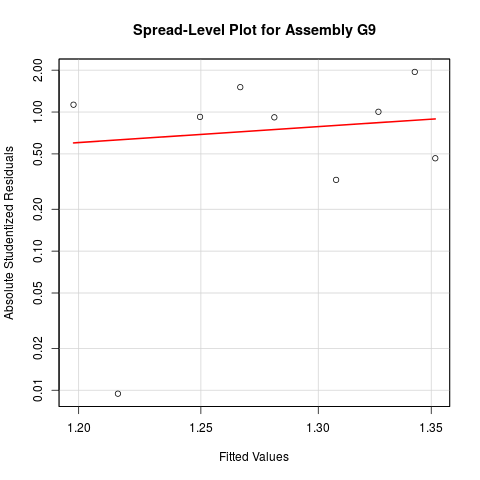
\includegraphics[keepaspectratio, width = 3.5 in]{figures/G9_slp.png}
\caption{Spread level plot for linear model applied to for assembly G9 in cycle 1.}
\label{fig:lm_G9_slp}
\end{figure}

While visual tests are subject to individual interpretation as to whether residuals are homoscedastic, statistical tests can be used to test for the same criteria. The Breusch-Pagan test, developed by Trevor Breusch and Adrian Pagan and independently suggested by Dennis R. Cook and Sanford Weisberg, tests for the heteroscedasticity in a linear regression model using a test statistic based on the chi-squared distribution \cite{breusch1979simple,cook1983diagnostics}. The null hypothesis states that the residuals in the linear regression model under consideration are homoscedastic, and if the calculated p-value $p<\alpha$, where $\alpha$ is the statistical significance level, then there is evidence to reject the null hypothesis. For this thesis, $\alpha$ is chosen at a level of 0.05, so a p-value less than this value means that there is a 95\% confidence level that the null hypothesis should be rejected. For the case of assembly G9, the calculated p-value is 0.56 so there is little evidence to suggest that the errors are heteroscedastic. A complete list of p-values for the Breusch-Pagan test for each assembly regression is shown in Table \ref{table:cyc1_pvalues}. From this table, it can be seen that 25 out of 28 assemblies pass the statistical test, which suggests that errors are homoscedastic for most assembly regressions.

\subsubsection*{Requirement 3: Independent residuals with respect to time}

Tests for independence of residuals are difficult to visualize, so this section will focus solely on statistical tests to determine whether residuals are correlated to each other. A common avenue for such analysis is to use the Durbin-Watson test for autocorrelation of disturbances \cite{durbin1950testing,faraway2014linear}. The null hypothesis states that the autocorrelation of the residuals is 0, implying independence of residuals. The test can be conducted for either positive correlation or negative correlation, so a two-sided test is conducted to test against the alternative hypothesis that the autocorrelation is not equal to 0. Once again, the null hypothesis is rejected for p-values less than 0.05, and Table \ref{table:cyc1_pvalues} indicates that most assemblies pass this test at the 95\% level, strongly suggesting that regressed residuals are independent from each other.

\subsubsection*{Requirement 4: Residuals exhibit a normal distribution centered around 0}

Residuals being normally distributed can be shown both graphically and statistically. Visually, a normal Quantile-Quantile (Q-Q) plot can be generated for the residuals to show normality \cite{faraway2014linear}. A Q-Q plot plots studentized residuals against theoretical quantiles of a normal distribution. The plotted points should fall along the line $y=x$, indicating that a specific quantile of residual lies exactly where the expected quantile from a normal distribution is. Figure \ref{fig:lm_G9_qq} shows an example of this for assembly G9, with the red line indicating a best fit line for the plotted data.

\begin{figure}[!htb]
\centering
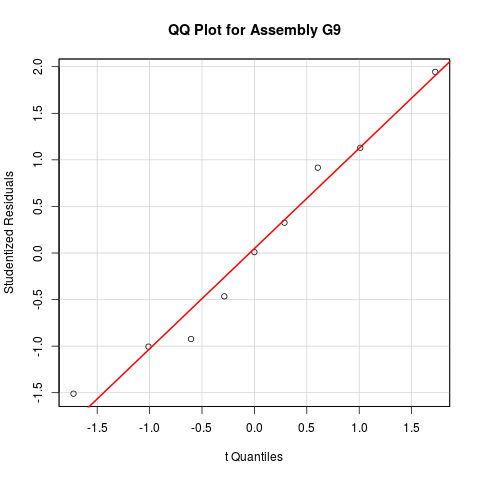
\includegraphics[keepaspectratio, width = 3.5 in]{figures/G9_qq.png}
\caption{Q-Q plot for linear model applied to for assembly G9 in cycle 1.}
\label{fig:lm_G9_qq}
\end{figure}

Once again, statistical tests can be utilized to test for normality in a more definitive manner. The Shapiro-Wilk test tests the null hypothesis that a sample distribution comes from a normally distributed population \cite{royston1982algorithm,royston1995remark,faraway2014linear}. It should be noted that the Shapiro-Wilk test does not assume the underlying sample distribution comes from a standard normal distribution, but instead tests for a general normal distribution with unknown population parameters. A complete list of p-values for each assembly when a linear regression is applied is shown once again in Table \ref{table:cyc1_pvalues}. For cycle 1, 27 out of the 28 assemblies resemble a normal distribution.

\begin{table}[!htb]
  \centering
  \begin{tabular}{DDDD}\toprule
      & \multicolumn{3}{l}{p-Values for Various Statistical Tests} \\ \midrule
     Assembly & Breusch-Pagan Test & Durbin-Watson Test & Shapiro-Wilk Test \\ \midrule
     G9 & 0.560 & 0.826 & 0.885 \\
     G8 & 0.783 & 0.630 & 0.325 \\
     B8 & 0.341 & 0.974 & 0.878 \\
     B9 & 0.033 & 0.398 & 0.488 \\
     E9 & 0.125 & 0.094 & 0.567 \\
     E8 & 0.089 & 0.694 & 0.895 \\
     F10 & 0.579 & 0.250 & 0.372 \\
     D10 & 0.176 & 0.458 & 0.249 \\
     B12 & 0.217 & 0.104 & 0.565 \\
     B13 & 0.381 & 0.310 & 0.240 \\
     B10 & 0.127 & 0.186 & 0.655 \\
     C9 & 0.954 & 0.738 & 0.000 \\
     C8 & 0.295 & 0.014 & 0.201 \\
     F8 & 0.593 & 0.460 & 0.518 \\
     F9 & 0.178 & 0.484 & 0.792 \\
     E11 & 0.523 & 0.412 & 0.933 \\
     E10 & 0.166 & 0.274 & 0.973 \\
     C13 & 0.043 & 0.110 & 0.122 \\
     C12 & 0.488 & 0.572 & 0.259 \\
     C11 & 0.964 & 0.044 & 0.082 \\
     C10 & 0.429 & 0.256 & 0.883 \\
     D12 & 0.931 & 0.082 & 0.419 \\
     A11 & 0.107 & 0.780 & 0.473 \\
     A10 & 0.057 & 0.344 & 0.203 \\
     A9 & 0.659 & 0.784 & 0.167 \\
     A8 & 0.049 & 0.102 & 0.150 \\
     D8 & 0.760 & 0.952 & 0.218 \\
     D9 & 0.206 & 0.752 & 0.906 \\ \bottomrule
  \end{tabular}
  \caption{Summary of p-values from statistical tests that test validity of linear regression model.}
  \label{table:cyc1_pvalues}
\end{table}

\subsubsection{Limitations of the Linear Model}\label{sec:lm_limitations}

In general, analysis of the conditions for a linear regression model indicates that linear models are quite adequate for first-order fitting purposes. Assuming that a linear model is indeed valid and RMS values shown in Figures \ref{fig:cyc1_lm_eighth_map} and \ref{fig:cyc2_lm_eighth_map} are indicative of the detection error, $\left(\delta_\phi/\phi \right)_{ij,detection}$ found in Equation \ref{eq:time_dep_unc}. A similar approach outlined in Section \ref{sec:unc_combine} can be followed that uses Equation \ref{eq:time_dep_unc} to find the 95\% value for detection uncertainty. Using the linear model, it is found that the 95\% CI for detection uncertainty is 1.9\% and 2.0\% for cycles 1 and 2 respectively.

While these 95\% CI values fit within the same error levels observed in section \ref{flux_map_unc}, there are assemblies in both cycles where a linear fit is inadequate, as evidenced by high assembly RMS values as well as cases where multiple statistical tests are rejected in favor of an alternative hypothesis. The primary reason for such behavior is due to the volatile power history for both cycles that call into question the steady-state requirements for linear fitting to be appropriate. Moreover, a linear fit cannot be conducted without knowing the BEAVRS reaction rates a prior, and neglects taking into account any of the actual operating conditions within the reactor. Thus, these limitations necessitate the use of more predictive models that can be used to capture higher-order effects observed within the reactor. section \ref{sec:cassim-unc} addresses such drawbacks by computing reaction rates from CASMO/Simulate to use as bases for comparison against BEAVRS data.

\subsection{Summary of Results}\label{sec:timeseries_summary}

 
This section serves to summarize the primary results from this task. Two models are used to compute detection uncertainty, namely the CASMO/Simulate model and the linear model. The 95\% confidence estimates of the UQ methods based on the CASMO/Simulate model and linear regression model are presented in Table \ref{table:results_complete_new}. Similarly, traditional methods for uncertainty quantification based on work from Section \ref{flux_map_unc} are also presented in Table \ref{table:results_complete_trad} for comparison. Theoretical analysis of axial uncertainties computes uncertainty using all measurements based on variations of signal strengths by groups. This approach determines uncertainties at each axial point using lookup tables and also sums each axial point and associated uncertainty to calculate axially integrated values. On the other hand, the multiple measurements method computes uncertainty for measurements based on repeated measurements that are conducted by the same detector in the same assembly at a given burnup.

It should be noted that results from the CASMO/Simulate model have been separated into two categories to show how much of the error stems from detection deviation and how much this error level increases after accounting for the uncertainty in using tilt-corrected data. The second column in Table \ref{table:results_complete_new} indicates the 95\% confidence interval of $\left(\delta_\phi/\phi\right)_{ij,detection}$ in Equation \ref{eq:time_dep_unc}, while the third column represents the 95\% confidence interval of the cumulative time-dependent uncertainty, $\left(\delta_\phi/\phi\right)_{ij,time-dep}$, which accounts for the uncertainty in using tilt-corrected data as well.

\begin{table}[!htb]
  \centering \raggedright
  \begin{tabular}{CCC}\toprule
      & \multicolumn{2}{l}{Traditional Methods of Uncertainty Quantification} \\ \midrule
      & Theoretical Analysis of Axial Uncertainties & Multiple Measurements\\ \midrule
     Cycle 1 & 1.4\% & 1.8\% \\ 
     Cycle 2 & 1.4\% & 1.5\% \\ \bottomrule
  \end{tabular}
  \caption{Summary of results from uncertainty quantification using traditional methods.}
  \label{table:results_complete_trad}
\end{table}

\begin{table}[!htb]
  \centering \raggedright
  \begin{tabular}{IHHH}\toprule
      & \multicolumn{3}{l}{Uncertainty Quantification Methods Based on Time Series Analysis} \\ \midrule
      & CASMO/Simulate Model (before tilt-correction UQ) & CASMO/Simulate Model (after tilt-correction UQ) & Linear Regression Model (after tilt-correction UQ) \\ \midrule
     Cycle 1 & 0.8\% & 1.8\% & 1.9\% \\ 
     Cycle 2 & 0.9\% & 1.9\% & 2.0\% \\ \bottomrule
  \end{tabular}
  \caption{Summary of results from uncertainty quantification using new methods based on time series analysis.}
  \label{table:results_complete_new}
\end{table}

Tables \ref{table:results_complete_trad} and \ref{table:results_complete_new} show that the uncertainty within the BEAVRS benchmark ranges from 1.4\% to 1.8\% in cycle 1 and 1.4\% to 1.9\% in cycle 2. These results indicate that time series analysis methods can be used to model time-dependent behavior, with measured data behaving in accordance with data from simulation tools. The CASMO/Simulate model, for example, predicts reaction rates based on operational conditions, and when accounting for the model bias, the time-dependent uncertainty produces uncertainty results on the same order as methods based on reaction rate map uncertainties. These findings are also independent of type of simulation model used to generate reaction rates. What is more, if uncertainties from using tilt-corrected data could be completely explained, then the remaining detection uncertainty from fitting the CASMO/Simulate model to BEAVRS data yield much lower errors than using traditional UQ methods. 

\clearpage


\bibliographystyle{unsrt}


\bibliography{uq_report}

\end{document}
